%%%%%%%%%%%%%%%%%%%%%%%%%%%%%%%%%%%%%%%%%%%%%%%%%%%%%%%%%%%%%%%%%%%%%%%%%%%%%
%                                                                           %
%   tuProlog 2.7 Documentation - 2012 edition                               %
%                                                                           %
%   E.Denti, January 2013                                                   %
%                                                                           %
%   Based on former contributions by A.Omicini, A.Ricci, G.Piancastelli     %
%%%%%%%%%%%%%%%%%%%%%%%%%%%%%%%%%%%%%%%%%%%%%%%%%%%%%%%%%%%%%%%%%%%%%%%%%%%%%

\documentclass[11pt]{report}
\usepackage[bookmarks=true,bookmarksopen=true,bookmarksnumbered]{hyperref}
\usepackage{graphicx}
\usepackage{color} % ED
\usepackage{fancyvrb}
\usepackage{caption}
%\usepackage{wrapfig}
%%%%%%%%%%%%%%%%%%%%%%%%%%%%
%\usepackage{float}
%\floatstyle{ruled}
%\newfloat{program}{thp}{lop}
%\floatname{program}{Program}
%%%%%%%%%%%%%%%%%%%%%%%%%%%%

\newcommand\xa[1]{\appendixname~\ref{app:#1}}
\newcommand\labelsec[1]{\label{sec:#1}}
\newcommand\xch[1]{\chaptername~\ref{ch:#1}}
\newcommand\xchp[1]{\chaptername~\ref{ch:#1} \onpagename~\pageref{ch:#1}}
\newcommand\xs[1]{\sectionname~\ref{sec:#1}}
\newcommand\xsp[1]{\sectionname~\ref{sec:#1} \onpagename~\pageref{sec:#1}}
\newcommand\labelssec[1]{\label{ssec:#1}}
\newcommand\xss[1]{\subsectionname~\ref{ssec:#1}}
\newcommand\xssp[1]{\subsectionname~\ref{ssec:#1} \onpagename~\pageref{ssec:#1}}
\newcommand\labelsssec[1]{\label{sssec:#1}}
\newcommand\xsss[1]{\subsectionname~\ref{sssec:#1}}
\newcommand\xsssp[1]{\subsectionname~\ref{sssec:#1} \onpagename~\pageref{sssec:#1}}
\newcommand\labelfig[1]{\label{fig:#1}}
\newcommand\xf[1]{\figurename~\ref{fig:#1}}
\newcommand\xff[2]{\figurenames~\ref{fig:#1}~and~\ref{fig:#2}}
\newcommand\xfp[1]{\figurename~\ref{fig:#1} \onpagename~\pageref{fig:#1}}
\newcommand\labeltab[1]{\label{tb:#1}}
\newcommand\xt[1]{\tablename~\ref{tb:#1}}
\newcommand\xtt[2]{\tablenames~\ref{tb:#1}~and~\ref{ab:#2}}
\newcommand\xtp[1]{\tablename~\ref{tb:#1} \onpagename~\pageref{tb:#1}}
\newcommand\labelenum[1]{\label{enum:#1}}
\newcommand\xen[1]{(\ref{enum:#1})}
\newcommand\xenp[1]{(\ref{enum:#1}) \onpagename~\pageref{enum:#1}}
%******************************************************************************%
\newcommand\bti[1]{\texttt{\textbf{#1}}}
\newcommand\bt[1]{\texttt{#1}}
\newcommand\template[1]{\textit{Template: }\texttt{#1}}
\newcommand\exception[1]{\textit{Exception: }\texttt{#1}}
\newcommand\ttit[1]{\texttt{\textit{#1}}}
%******************************************************************************%
\newcommand{\LIA}{\mbox{\textsf{LIA}}}
\newcommand{\aclt}{\mbox{$\mathcal{ACLT}$}}
\newcommand{\respect}{\mbox{\sf{{R}e{S}pec{T}}}}
\newcommand{\luce}{\mbox{\sf{{L}u{C}e}}}
\newcommand{\tucson}{\mbox{\sf{{T}u{CS}o{N}}}}
\newcommand{\alice}{\mbox{\sf{{aliCE}}}}
\newcommand{\apice}{\mbox{\sf{{APICe}}}}
\newcommand{\tuprolog}{\mbox{{\sf{tu}}Prolog}}
%******************************************************************************%
\newcommand\version[1]{\mbox{Document revision: #1}}
\newcommand\creationdate[1]{\mbox{Creation date: #1}}
\newcommand\lastchangesdate[1]{\mbox{Last Changes date: #1}}
\newcommand\noa[2]{\noindent\emph{Note of the author (#1): }#2\\\\}
\newcommand\logo{
    \begin{figure}[tp]
        \begin{center}
            
\includegraphics[width=5cm]{images/logo}
        \end{center}
\end{figure}
}
%******************************************************************************%
\newcommand{\classname}[1]{\texttt{#1}}
\newcommand{\varname}[1]{\texttt{#1}}
\newcommand{\predicate}[1]{\texttt{#1}}
\newcommand{\code}[1]{\texttt{#1}}
\newcommand{\keycap}[1]{\textbf{#1}}
\newcommand{\guibutton}[1]{\textsf{#1}}
\newcommand{\userinput}[1]{\texttt{#1}}
\newcommand{\figref}[1]{\figurename~\ref{#1}}
%******************************************************************************%
\title{{\Huge{\bf{\tuprolog{} Manual\\\mbox{ }\\}}}
        \tuprolog{} version: 2.7.1\\\mbox{ }\\
{\small\today\\}
}
\author{ \mbox{ }\\ \textsc{Enrico Denti}\\Alma Mater Studiorum--Universit\`{a} di Bologna, Italy
}

\date{}

\setcounter{secnumdepth}{4}
\setcounter{tocdepth}{4}

\begin{document}

\logo

\maketitle

\tableofcontents

%******************************************************************************%
%=======================================================================
\chapter{What is \tuprolog{}}
\label{what-is}
%=======================================================================

\tuprolog{} is an open-source, light-weight Prolog framework for distributed applications and infrastructures, released under the LGPL license, available from \url{http://tuprolog.apice.unibo.it}.

Originally developed in/upon Java, which still remains the main reference platform,
\tuprolog{} is currently available for several platforms/environments:
\begin{itemize}
  \item plain JavaSE;
  \item Eclipse plugin;
  \item Android;
  \item Microsoft .NET.
\end{itemize}
%
While they all share the same core and libraries, the latter features an \emph{ad hoc} library which extends the multi-paradigm approach to virtually any language available on the .NET platform (more on this in Section \xch{dotnet}).

Unlike most Prolog programming environments, aimed at providing a very efficient (yet monolithic) stand-alone Prolog system, \tuprolog{} is explicitly designed to be \emph{minimal}, dynamically \emph{configurable}, straightforwardly \emph{integrated} with Java and .NET so as to naturally support multi-paradigm/multi-language programming (MPP), and \emph{easily deployable}.

\textit{Minimality} means that its core contains only the Prolog engine essentials -- roughly speaking, the resolution engine and some related basic mechanisms -- for as little as 155KB: any other feature is implemented in \textit{libraries}.
%
So, each user can customize his/her prolog system to fit his/her own needs, and no more:
this is what we mean by \tuprolog{} \textit{configurability}---the necessary counterpart of minimality.

Libraries provide packages of predicates, functors and operators, and can be loaded and unloaded in a \tuprolog{} engine both statically and dynamically.
%
Several standard libraries are included in the \tuprolog{} distribution, and are loaded by default in the standard \tuprolog{} configuration; however, users can easily develop their own libraries either in several ways -- just pure Prolog, just pure Java\footnote{The .NET version of \tuprolog{} supports other languages available on the .NET platform: more on this topic in Section \xch{dotnet}}, or a mix of the two --, as we will discuss in \xch{howto-develop-libraries}.

\textit{Multi-paradigm programming} is another key feature of \tuprolog{}.
%
In fact, the \tuprolog{} design was intentionally calibrated from the early stages to support a straightforward, pervasive, multi-language/multi-paradigm integration, so as to enable users to:
\begin{itemize}
  \item using any Java\footnote{For the .NET version: any .NET class, library, object, etc.} class, library, object \emph{directly from the Prolog code}
  (\xch{java-library}) with no need of pre-declarations, awkward syntax, etc., with full support of parameter passing from the two worlds, yet leaving the two languages and computational models totally separate so as to preserve \emph{a priori} their own semantics---thus bringing the power of the object-oriented platform (e.g. Java Swing, JDBC, etc) to the Prolog world for free;

  \item using any Prolog engine \emph{directly from the Java/.NET code} as one would
   do with any other Java libraries/.NET assemblies, again with full support of parameter passing from the two worlds in a non-intrusive, simple way that does not alter any semantics---thus bringing the power of logic programming into virtually \emph{any} Java/.NET application;

  \item augmenting Prolog by defining new libraries \xch{howto-develop-libraries})
  either in Prolog, or in the object-oriented language of the selected platform (again, with a straightforward, easy-to-use approach based on reflection which avoids any pre-declaration, language-to-language mapping, etc), or in a mix of both;

  \item augmenting Java\footnote{This feature is currently available only in the Java version: a suitable extension to the .NET platform is under study.} by defining new Java methods in Prolog (the so-called `P@J' framework---\xch{PJ}), which exploits reflection and type inference to provide the user with an easy-to-use way to implement Java methods declaratively.
\end{itemize}

Last but not least, \textit{easy deployability} means that the installation requirements are minimal, and that the installation procedure is in most cases\footnote{Exceptions are the Eclipse plugin and the Android versions, which need to be installed as required by the hosting platforms.} as simple as copying one archive to the desired folder.
%
Coherently, a Java-based installation requires only a suitable Java Virtual Machine, and `installing' is just copying a single JAR file somewhere---for as much as 474KB of disk usage (yes, minimality is not just a claim here).
%
Of course, other components can be added (documentation, extra libraries, sources..), but are not necessary for a standard everyday use.
%
The file size is quite similar for the Android platform -- the single APK archive is 234KB -- although an Android-compliant install is performed due to Android requirements.
%
The install process is also quite the same on the .NET platform, although the files are slightly larger.
%
The Eclipse platform also requires a different procedure, since plugin installation have to conform to the requirements of the Eclipse plugin manager: consequently, an update site was set up, where the \tuprolog{} plugin is available as an Eclipse feature. Due to these constraints, file size increases to 1.5MB.


In order to manage all these platforms in a uniform way, a suitable \emph{version numbering scheme} was recently introduced:
\begin{itemize}
  \item the fist two digits represent the engine version;
  \item the last (third) digit is platform-specific and accounts for version differences which do not impact on the Prolog engine -- that is, on the
      \tuprolog{} behaviour -- but simply on graphical aspects or platform-specific
      issues or bugs.
\end{itemize}
%
So, as long as the first two digits are the same, a \tuprolog{} application is guaranteed to behave identically on any supported platform.


Finally, \tuprolog{} also supports \textit{interoperability} with both Internet standard patterns (such as TCP/IP, RMI, CORBA) and coordination models and languages.
%
The latter aspect, in particular, is currently developed in the context of the \tucson{} coordination infrastructure \cite{tucson-aamas99,respect-scico2001}, which provides logic-based, programmable tuple spaces (called \emph{tuple centres}) as the coordination media for distributed processes and agents.\footnote{An alternative infrastructure, \luce{} \cite{luce-aamas2001}, developed the same approach in a location-unaware fashion: this infrastructure is currently no longer supported.}



%******************************************************************************%
%=====================================================================
\chapter{Installing \tuprolog{}}
\label{installation}
%=====================================================================

Quite obviously, the installation procedure depends on the platform of choice.
For Java, Microsoft .NET and Android, the first step is to manually download the desired distribution (or even just the single binary file) from the \tuprolog{} web site, \texttt{tuprolog.alice.unibo.it}, or directly from the Google code repository, \texttt{tuprolog.googlecode.com}; for Eclipse the procedure is different, since the plug-in installation has to be performed via the Eclipse Plugin Manager.

As a further alternative, users wishing to have a look at \tuprolog{} and trying it without installing anything on their computer can do so by exploiting the `Run via Java Web Start' option, available on the \tuprolog{} web site.

\section{Installation in Java}

The complete Java distribution has the form of a single \texttt{zip} file which contains everything (binaries, sources, documentation, examples, etc.) and unzips into a multi-level directory tree, similar to the following (only first-level sub-dirs are shown):

\begin{Verbatim}[frame=single, framerule=0.5mm, samepage=true, boxwidth=5cm]
    2p
    |---ant
    |---bin
    |---build
    |   |---archives
    |   |---classes
    |   |---release
    |   |---reports
    |   |---tests
    |---doc
    |   |---javadoc
    |---lib
    |---src
    |---test
    |   |---fit
    |   |---unit
    |---tmp
    |---test
\end{Verbatim}

An alternative distribution, without sources, is also available in the \textit{Download} section of the \tuprolog{} repository: obviously, in this case only a subset of the above folders is present (namely, only \texttt{bin}, \texttt{doc}, \texttt{lib} and \texttt{reports}).

If you are only interested in the Java binaries, just look into the \texttt{build/archives} directory, which contains two JAR files:
%
\begin{itemize}
%
\item \texttt{2p.jar}, which contains everything you need to use \tuprolog{},
  such as the core API, the \texttt{Agent} application, libraries, GUI,
  etc.; this is a runnable JAR, that open the \tuprolog{} IDE when double-clicked.
%
\item \texttt{tuprolog.jar}, which contains only the core part of \tuprolog{},
  namely, what you will need to include in a Java application project to be able to access the \tuprolog{} classes, and write multi-paradigm Java/Prolog applications.
\end{itemize}

The other folders contain project-specific files: \texttt{src} contains all the sources, \texttt{doc} all the documentation, \texttt{lib} the libraries used by the \tuprolog{} project, \texttt{test} the sources for the \tuprolog{} test suite (partly as FIT test, partly as JUnit tests), \texttt{ant} some Ant scripts to automate the build of parts of the \tuprolog{} project, etc.


\section{Installation in .NET}

The complete .NET distribution has also the form of a single \texttt{zip} file containing everything; however, due to the automatic generation of \tuprolog{} .NET binaries via IKVM from Java (more on this in Chapter \ref{ch:mpp-in-dotnet}), the unzipped directory tree is simpler, as there are no sources (and therefore no tests, no ant tasks, etc), except for \texttt{OOLibrary} and Conventions, which are NET-specific and therefore written in C\#.
%
So, the resulting tree is similar to the following:
%
\begin{verbatim}
    2p
    |---build
    |   |---examples
    |   |---lib
    |---OOLibrary
    |   |---Conventions
    |   |---Fixtures
    |   |---OOLibrary
\end{verbatim}
%
Here, too, an alternative distribution, without the OOLibrary and conventions sources, is also available in the \textit{Download} section of the \tuprolog{} repository: again, only a subset of the above folders is present in this case.

The .NET binary, \texttt{2p.exe}, can be found in the \texttt{build} folder.


\section{Installation in Android}

The Android distribution has the form of a single \texttt{apk} file, to be installed via install mechanism provided by the Android OS.
So, unless you are interested in the implementation details, there should be no need to download the whole project distribution.
If, however, you like to do so, you will eventually get to a directory tree similar to the following (only the most relevant first-level sub-folders are shown):
%
\begin{verbatim}
    2p
    |---assets
    |---bin
    |   |---classes
    |   |---res
    |---doc
    |---gen
    |---libs
    |---res
    |---screenshots
    |---src
\end{verbatim}
%
The APK binary can be found into the \texttt{bin} folder.

As for the Java case, the other folders contain project-specific files: in particular, \texttt{src} contains the sources, \texttt{res} the Android resources automatically generated during the project build process, \texttt{libs} the libraries used by this project---mainly, the \texttt{tuprolog.jar} file of the corresponding Java version, imported here as an external dependency.


\section{Installation in Eclipse}

The installation procedure is different for the Eclipse platform due to the need to conform to the Eclipse standard procedure for plug-in installation via Plugin Manager.
Please see the specific section on the \tuprolog{} web site for detailed, screenshot-driven instruction. 
%******************************************************************************%
%=======================================================================
\chapter{Getting Started}
\label{ch:getting-started}
%=======================================================================

\tuprolog{} can be enjoyed from different perspectives:
\begin{enumerate}
  \item as a \textit{Prolog user}, you can exploit its Integrated Development
        Environment (IDE) and Graphical User Interface (GUI) to consult, edit, and run Prolog programs, as you would do with any other Prolog system---and you can do so in any of the supported platforms (Java, .NET, Android, Eclipse).
  \item as a \textit{Java user}, you can include \tuprolog{} in any Java project, in Eclipse or any other IDE of your choice,
        thus bringing the power of Artificial Intelligence to the Java world; the \tuprolog{} API provides many classes and methods for exchanging data between the Java and the Prolog worlds.
        If your goal is to build a hybrid Java+Prolog application to be run from the Prolog side, the \tuprolog{} plugin
        for Eclipse is probably the most practical choice, as the \tuprolog{} perspective provides all the views over the Prolog world in an Eclipse-compliant, effective way.
  \item as a \textit{.NET user}, analogously, you can add \tuprolog{} to any
        Visual Studio project (including the related IKVM libraries, as detailed in Chapter \ref{ch:mpp-in-dotnet}, or just manually compile your .NET application with the necessary DLL files in the build path. The \tuprolog{} API, which is nearly identical to the Java one, provides for proper data exchange
        between the .NET and the Prolog worlds.
  \item finally, as an \textit{Android user}, you can both enjoy the \tuprolog{} app
        to consult, edit, and run Prolog programs, as you would do with any other Prolog system, and --perhaps more interestingly-- exploit the \tuprolog{} Java API for developing Android applications, adding intelligence to your next Android app.
\end{enumerate}

%=======================================================================
\section{\tuprolog{} for the Prolog User}
\label{sec:prolog-user-perspective}
%=======================================================================

As a Prolog user/programmer, you might want to start running your existing programs.
%
There are three ways to do so:
\begin{itemize}
  \item by using the graphical \tuprolog{} GUI (both in Java and .NET)
  \item by using the console-based \tuprolog{} CUI  (Java only)
  \item by using the \texttt{Agent} class to execute a Prolog program in a `batch' form---that is, running the program provided as a text file (Java only).
\end{itemize}

The first two forms are rather obvious: after starting the GUI/CUI, you will get a rather standard graphical/character-based Prolog user interface (Figure \ref{fig:tuprologGUICUI}).

The GUI includes an editing pane with syntax highlighting, a toolbar providing facilities to load/save/create theories, load/unload libraries, and show/hide the the debug information window; at the bottom, the status bar provides information, as detailed below.

The GUI can be launched either by double-clicking the \tuprolog{} executable (\texttt{2p.jar} in Java, \texttt{2p.exe} in .NET), or by manually issuing the commands

\texttt{java -cp \emph{dir}/2p.jar alice.tuprologx.ide.GUILauncher}

\noindent or

\texttt{2p.exe}

\noindent in .NET, respectively.

Analogously, the command-line CUIconsole (available in Java only) can be launched by issuing the command:

\texttt{java -cp \emph{dir}/2p.jar alice.tuprologx.ide.CUIConsole}

\noindent The CUIconsole can be quitted issuing the standard \texttt{halt.} command.

% ED 2.7.3
\begin{figure}
\centering
  \includegraphics[width=300px]{images/tuprologIDE.png}\\
  \includegraphics[width=300px]{images/tuprologCUI.png}\\
  \caption{The standard \tuprolog{} GUI and CUI. (The upper right button, opening SpyFrame window, is present only from version 2.7.2 onwards; the \textit{call tree} tab view in the bottom dialog is to be included in version 2.7.3).}\label{fig:tuprologGUICUI}
\end{figure}

The third form, available in Java only, is basically an auxiliary tool to batch-execute a Prolog program: it takes the name of a text file containing a Prolog theory as its first (mandatory) argument and optionally the goal to be solved as its second argument, then starts a new Prolog virtual machine, performs the demonstration, and ends.
%
The \texttt{Agent} tool is invoked from the command line as follows:

\texttt{java -cp \textit{dir}/2p.jar alice.tuprolog.Agent \textit{theoryfile}
\{\textit{goal}\}}

\noindent For instance, if the file \verb|hello.pl| contains the mini-theory:

\texttt{go :- write('hello, world!'), nl.}

\noindent the following command causes its execution:

\texttt{java -cp \textit{dir}/2p.jar alice.tuprolog.Agent hello.pl go.}

\noindent resulting in the string \texttt{hello, world!} being printed on the standard output.

\noindent Alternatively, the goal to be proven can be embedded in the Prolog source by means of the \texttt{solve} directive, as follows (Figure \ref{fig:tuprologAgent}):

\texttt{:- solve(go).}\\
\indent\texttt{go :- write('hello, world!'), nl.}

\noindent Quite obviously, in this case no second argument is required.

\begin{figure}
\centering
  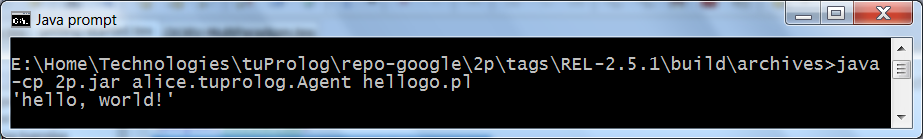
\includegraphics[width=300px]{images/tuprologAgent.png}
  \caption{The \tuprolog{} Agent tool.}\label{fig:tuprologAgent}
\end{figure}

%------------------------------------------------------
\subsection{Editing theories}
\label{sec:editing-theories}
%------------------------------------------------------

The editing area allows multiple theories to be created and modified at the same time, by allocating a tab with a new text area for each theory.
%
The text area provides syntax highlighting for comments, string and list literals, and predefined predicates.
%
Undo and Redo actions are supported through the usual \keycap{Ctrl}+\keycap{Z} and \keycap{Ctrl}+\keycap{Shift}+\keycap{Z} key bindings.

\begin{figure}
\centering
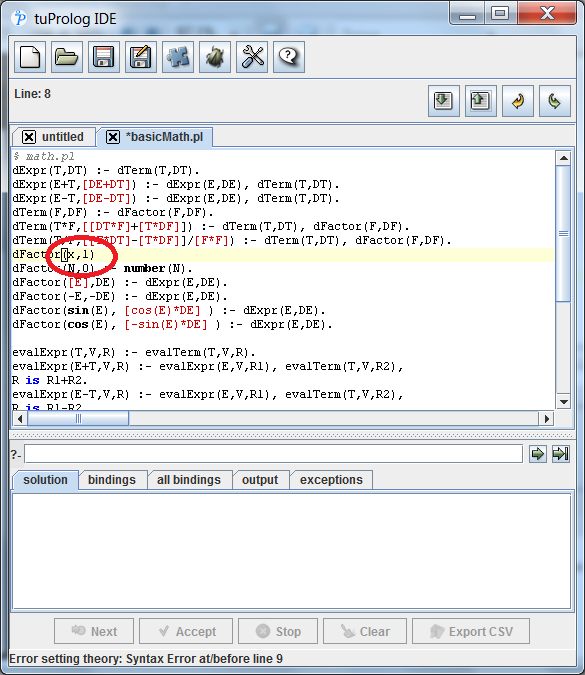
\includegraphics[width=7cm]{images/syntaxErrorFound}
\caption{Syntax error found when setting a theory.}
\label{fig:syntax-error-found}
\end{figure}

\begin{figure}
\centering
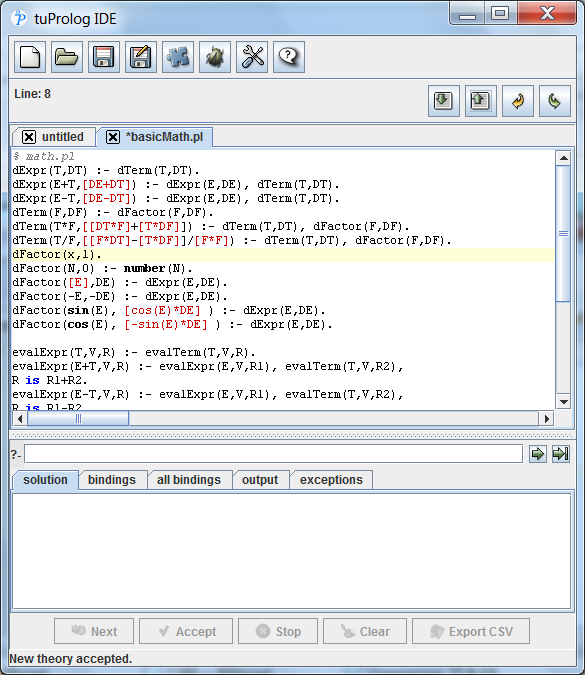
\includegraphics[width=7cm]{images/setTheorySucceeded}
\caption{Set theory operation succeeded.}
\label{fig:set-theory-succeeded}
\end{figure}

The toolbar contains four buttons: two are used to upload/download a theory to/from the Prolog engine, two support the classical Undo/Redo actions.
%
Explicit uploading/downloading of theories to/from the Prolog engine is a consequence of \tuprolog{}'s choice to maintain a clear separation between the engine and the currently-viewed theories: in this way,
\begin{itemize}
  \item theories can be edited without affecting the engine content: they can also be in an inconsistent state, since syntax checking is performed only upon loading;
  \item changes in the current database performed by the Prolog program via the \texttt{assert}/\texttt{retract} do not affect the theory shown in the editor, which maintains the original user theory.
\end{itemize}
%
Accordingly, the \textit{set theory} button uploads the text in the editor window to the engine, while the \textit{get theory} button downloads the current engine theory (possibly changed by the program) from the engine to a new editor tab.

However, for the user convenience, a logical shortcut is provided that automatically uploads the current theory to the engine whenever a new query is issued: obviously, if the theory is invalid, the query will not be executed.
%
Manual uploading is still needed whenever the theory in the editor window is modified via other other means than the built-in editor---for instance, after a \predicate{consult/1} goal\footnote{%
  If a Prolog theory contains an \texttt{include} directive or a \texttt{consult} command to load other sub-files,
  \tuprolog{} versions up to 2.6 require either the absolute sub-file name, or a relative path referred to the engine's
  base folder. From version 2.7 on, an enhanced mechanism enables a Prolog file located in \texttt{someOtherFolder} (that is, a folder other than the current one) to consult/include another file from the current
  folder by simply issuing a \texttt{consult(someOtherFile)} command, delegating the \tuprolog{} engine for searching the file in all the subfolders of the current working folder. See also Section \ref{ssec:relative-paths-consulting-subfiles-in-java-project}.
}, or via other editors.

The status bar at the bottom of the window reports information such as the cursor line number or syntax errors when setting an invalid theory.
%
For instance, Figure \ref{fig:syntax-error-found} shows the error message due to a missing dot at line 8, while Figure \ref{fig:set-theory-succeeded} shows the status message after the error has been corrected, and the theory successfully uploaded.

%------------------------------------------------------
\subsection{Solving goals}
\label{sec:solving-goals}
%------------------------------------------------------

The console at the bottom of the window contains the \textit{query textfield} and a multi-purpose, tabbed information panel.

The \textit{query textfield} is where to write and execute queries: the leftmost (\guibutton{Solve}) button triggers the engine to find the first (and then the subsequent) solution(s) interactively, while the rightmost (\guibutton{Solve All}) button forces the engine to find all the solutions at once.
%
Pressing the \keycap{Enter} key in the textfield has the same effect as pressing the \guibutton{Solve} button.

\begin{figure}
\centering
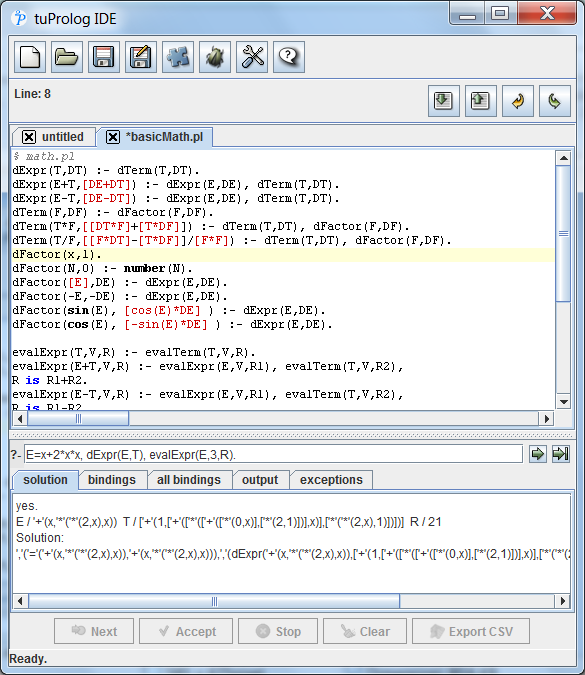
\includegraphics[width=7cm]{images/gui-solutions}
\caption{The solutions tab showing the query solution.
(The \textit{call tree} tab view is to be included in version 2.7.3).}
% 2.7.3
\label{fig:gui-solutions}
\end{figure}

\begin{figure}
\centering
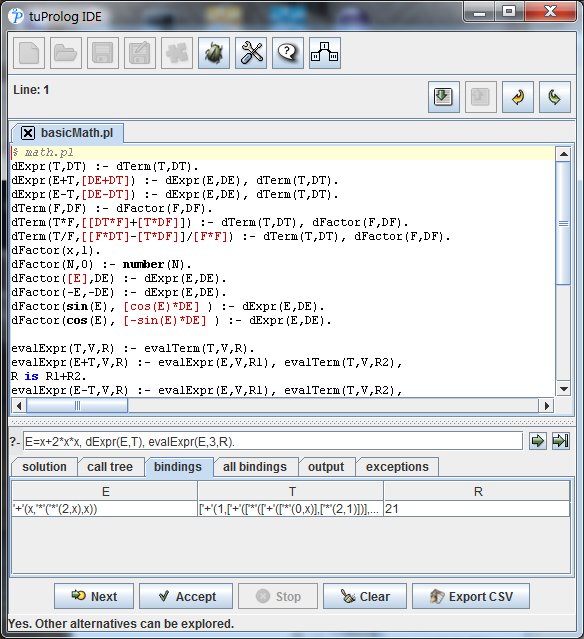
\includegraphics[width=7cm]{images/gui-bindings}
\caption{The bindings tab showing the bindings of query solution.
(The \textit{call tree} tab view is to be included in version 2.7.3).}
% 2.7.3
\label{fig:gui-bindings}
\end{figure}

The subsequent area below contains six panes:
%
\begin{itemize}
\item the \textit{solution} pane shows the query solutions (see Figure \ref{fig:gui-solutions}): proper control buttons are provided to iterate through multiple solutions;

% 2.7.3
% \item the \textit{call tree} pane shows a graphical view of the last-solved query (see Figure \ref{fig:gui-calltree});

\item the \textit{binding} and the \textit{all bindings} panes show the variable bindings in tabular form, for a single solution or for all solutions, respectively (see Figure \ref{fig:gui-bindings}); here, too, proper control buttons are provided to clear the bindings pane and export the tabular data in a convenient CSV format;

\item the \textit{output} pane shows the output performed by the program via \texttt{write} and other console I/O predicates (Figure \ref{fig:gui-output}).
    Please note that output performed by Java methods -- that is, methods invoked on Java objects via \classname{JavaLibrary} -- are \textit{not} captured and displayed in this view: for further information on this topic, refer to Section \ref{sec:java-library}.
    %
    Again, control buttons are provided to clear the output pane.

\item the \textit{exceptions} pane shows the exceptions raised during the query demonstration: if exceptions are triggered, it gains focus automatically and is color-highlighted for the user convenience (Figure \ref{fig:gui-exceptions}).
\end{itemize}

% 2.7.3
%\begin{figure}
%\centering
%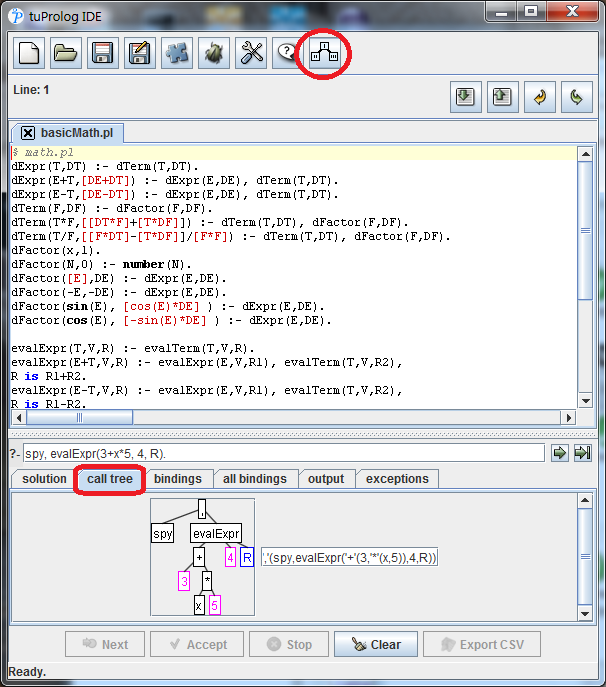
\includegraphics[width=7cm]{images/gui-calltree1}
%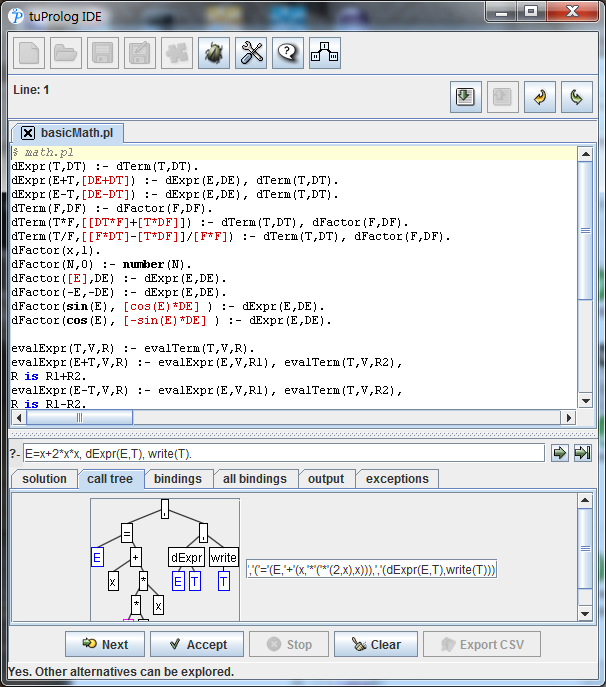
\includegraphics[width=7cm]{images/gui-calltree2}
%\caption{The call tree tab showing a graphical view of the last-solved query.}
%\label{fig:gui-calltree}
%\end{figure}

\begin{figure}
\centering
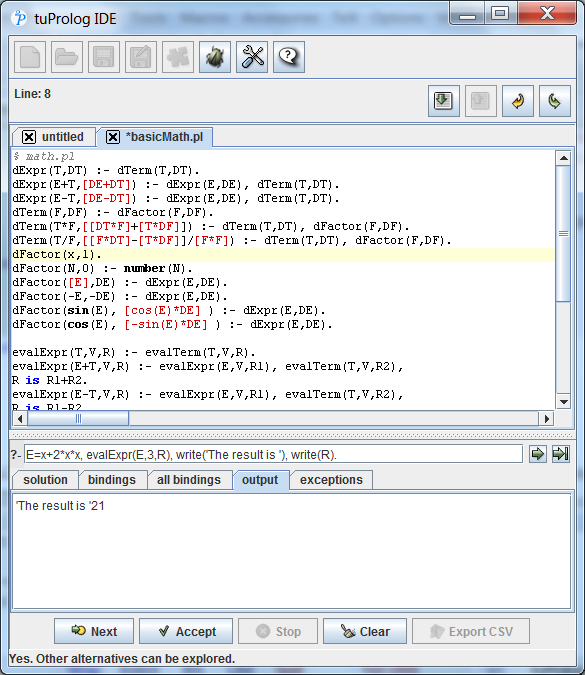
\includegraphics[width=7cm]{images/gui-output}
\caption{The output tab showing the query printing.
(The \textit{call tree} tab view is to be included in version 2.7.3).}
% 2.7.3
\label{fig:gui-output}
\end{figure}

\begin{figure}
\centering
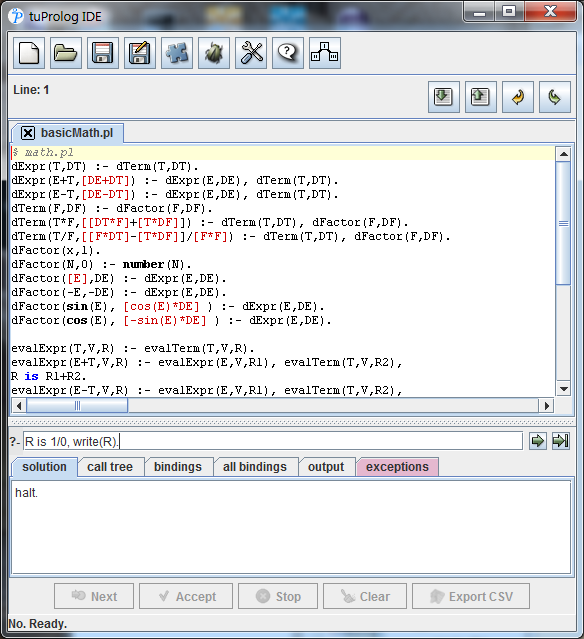
\includegraphics[width=7cm]{images/gui-exceptions}
\caption{The exceptions tab gaining focus and showing raised exceptions.
(The \textit{call tree} tab view is to be included in version 2.7.3).}
% 2.7.3
\label{fig:gui-exceptions}
\end{figure}
Query and answers are stored in chronological order, and can be explored by means of \keycap{Up} and \keycap{Down} arrow keys from the query input textfield.

The \guibutton{Stop} button makes it possible to stop the engine if a computation takes too long or a bug in the theory is causing an infinite loop.
%(Note: like most Prolog systems, \tuprolog{} does not normally perform \textit{occur check}, for performance reasons; this check can be enabled via the proper built-in predicate---see Section \ref{sec:basic-library} for details.)

With respect to this issue, it is worth noting that, unlike most Prolog systems, \tuprolog{} performs the so-called \textit{occur check} systematically: so, \texttt{unify\_with\_occurs\_check/2} and \texttt{=/2} behave identically (see Section \ref{sec:basic-library}).

%------------------------------------------------------
\subsection{Debugging support}
\label{ssec:debugging-support}
%------------------------------------------------------

Debug support in \tuprolog{} is actually limited compared to other professional Prolog systems: however, \textit{warnings} and \textit{spy information} are available.

To this end, the \guibutton{View Debug Information} button opens the Debug window which lists \textit{i)} all the warnings, produced by events such as the attempt of redefining a library predicate, and \textit{ii)} the step-by-step spy information of the engine computation during a goal demonstration.

Warnings are always active, while spy notification has to be explicitly enabled (and disabled) via the built-in \predicate{spy/0} (\predicate{nospy/0}) predicate.
%
Figure \ref{fig:gui-debug} shows an example of spy information for a goal: by default, information is presented in a collapsed form, but single nodes (or all the nodes) can be expanded using the toolbar buttons, to access more detailed information.

\begin{figure}
\centering
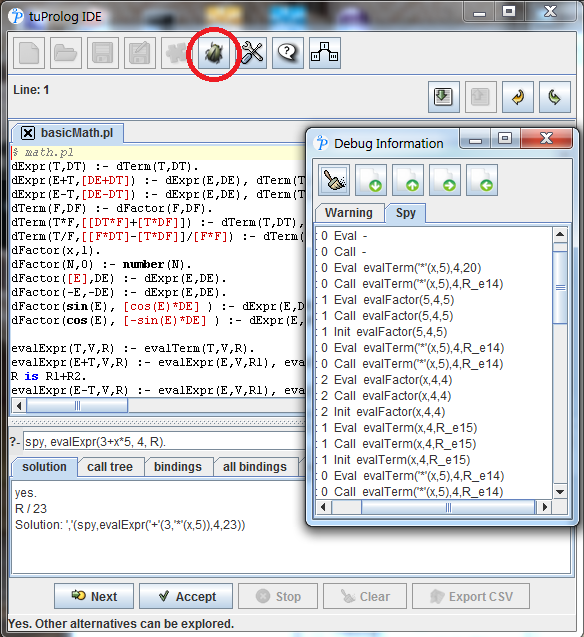
\includegraphics[width=7cm]{images/gui-debug}
\caption{Debug Information View after the execution of a goal.}
\label{fig:gui-debug}
\end{figure}

As of \tuprolog{} 2.7.2, an alternative approach is available via the \textit{Spy Frame} window, which can be opened clicking on the top-right, tree-like button (Figure \ref{fig:gui-spyframe}).
This window makes it possible to \textit{graphically reproduce} the solving process of the query, step-by-step: so, while the above debug view operates in real time during the resolution, the SpyFrame operates \textit{after} the query has been solved, basically re-solving the same query one step at a time\footnote{%
    SpyFrame exploits its own Prolog engine and execution thread for this purpose, so no side effects are caused in the main window even if the SpyFrame is closed unexpectedly.}
%
Each time the Next button is pressed, the simulation advances of \textit{N} steps, where \textit{N} is the number shown in the adjacent textfield (default 1).
Figure \ref{fig:gui-spyframe} shows some screenshots captured in different phases of a rather complex demonstration.

\begin{figure}
\centering
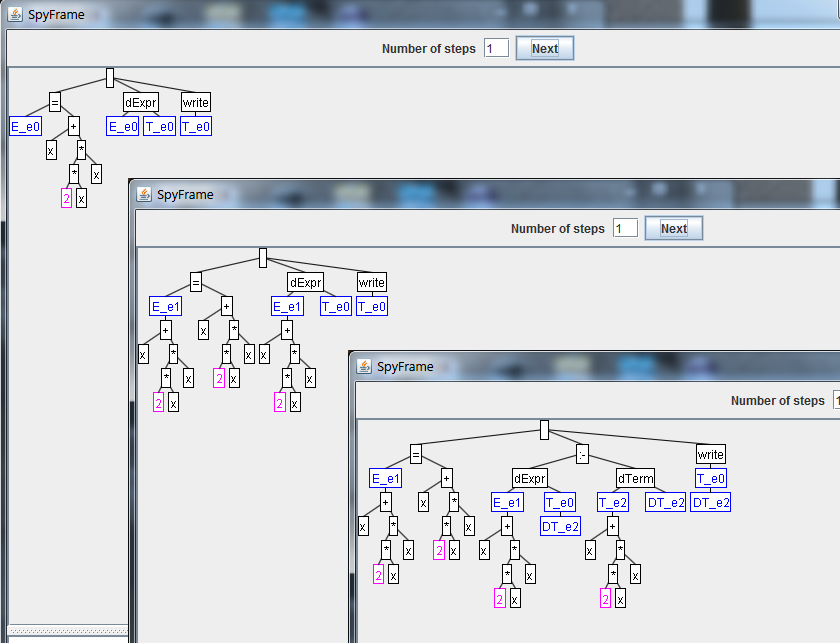
\includegraphics[width=7cm]{images/gui-spyframe1}
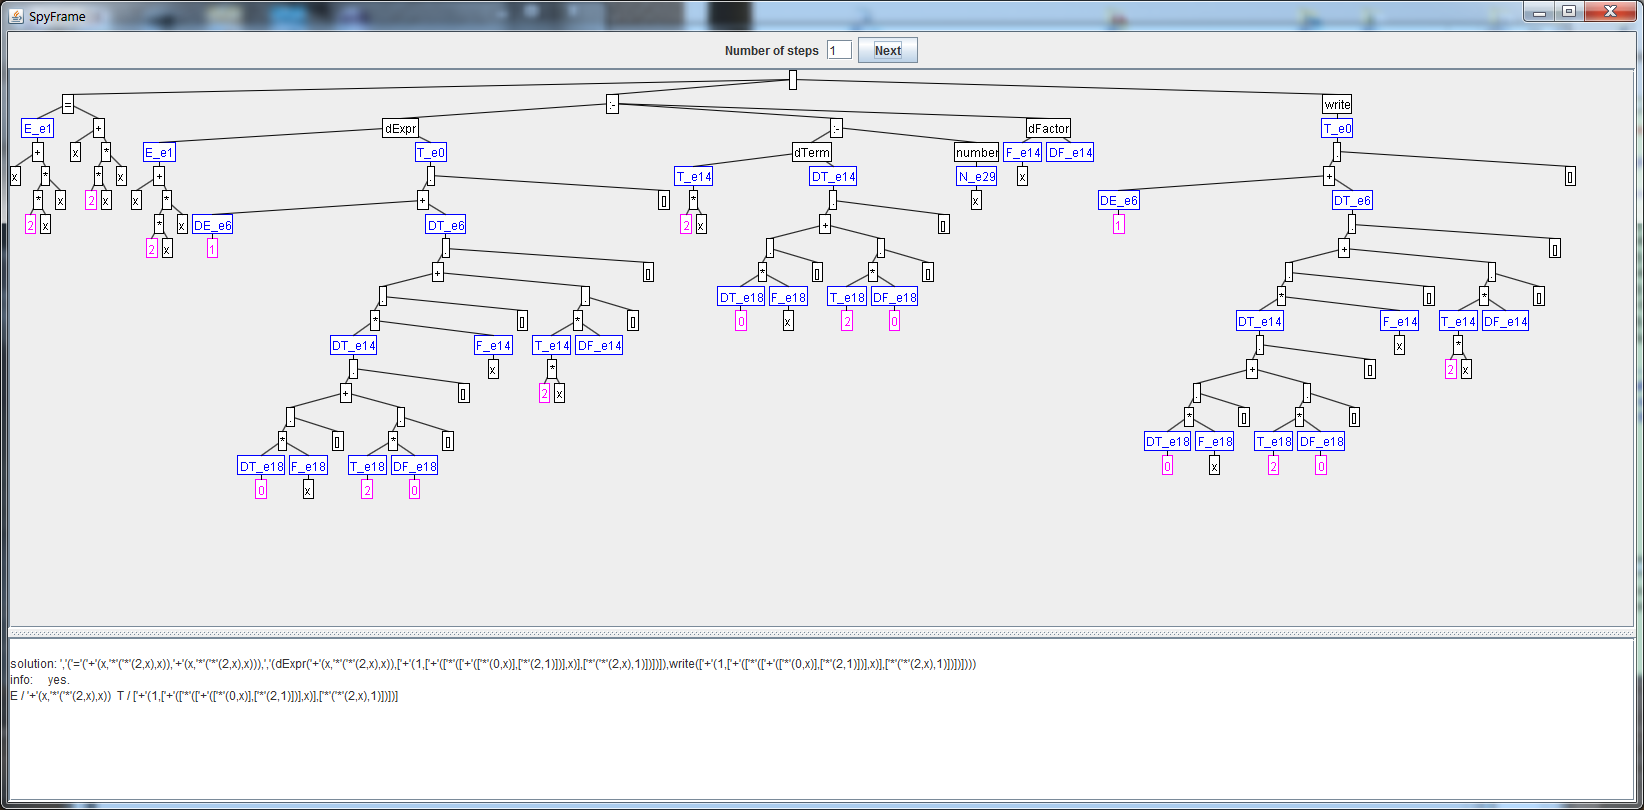
\includegraphics[width=7cm]{images/gui-spyframe2}
\caption{The Spy Frame (new in \tuprolog{} 2.7.2) showing a step-by-step graphical view of the last-solved query.}
\label{fig:gui-spyframe}
\end{figure}


%------------------------------------------------------
\subsection{Dynamic library management}
\label{ssec:dynamic-library-management}
%------------------------------------------------------

As anticipated above, \tuprolog{} engines are dynamically extensible via \textit{libraries}: each library can provide its own set of new built-in
predicates and functors, as well as a related theory.
%
By default, the standard set of libraries is loaded into any newly-created engine, but the library set of each engine can be easily modified via the \textit{Library Manager}, which is displayed by pressing the \guibutton{Open Library Manager} button in the toolbar (Figure \ref{fig:gui-library-manager}).

\begin{figure}
\centering
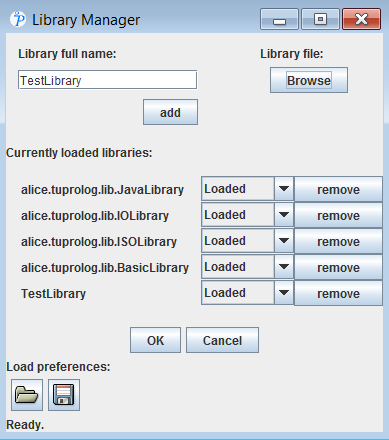
\includegraphics[width=7cm]{images/gui-library-manager}
\caption{The Library Manager window.}
\label{fig:gui-library-manager}
\end{figure}

This dialog displays the list of the currently loaded libraries---by default,
\classname{BasicLibrary}, \classname{IOLibrary}, \classname{ISOLibrary}, \classname{JavaLibrary}.
%
Other libraries can be added by providing the fully qualified name of the library class in the textfield, and pressing the \guibutton{Add} button: the added library will be displayed with an initial \textit{Unloaded} status.
The new library must be in the current class path for \tuprolog{} to find it; alternatively, the \textit{Browse..} button can be used to locate a library class anywhere in the file system (furhter information on class loading issues can be found in Section \ref{ssec:library-loading-issues}).
%
Quite clearly, class loading constraints also apply to any further class possibly needed by the library, too: a library will not be added to the manager/loaded into the engine if any of its required classes cannot be found.

The library manager takes into account the effects of \verb|load_library/1|-\verb|/2| and \verb|unload_library/1|-\verb|/2| predicates/directives, too: so, for instance, after a goal such as \verb|load_library('TestLibrary'), test(X).|, a new entry for \verb|TestLibrary| would be displayed.

If a library cannot be added, or its loading into the engine fails (for instance, due to an invalid class name, or the class not being in the current class paths, or a class not extending the \classname{alice.tuprolog.Library} class, etc.), an error message will be displayed in the status bar.

The bottom icons in Figure \ref{fig:gui-library-manager} are used to load and store preferences.

\noindent Finally, the \guibutton{config} button in the \tuprolog{} GUI opens the configuration dialog (Figure \ref{fig:gui-configuration}), which provides access to a set of options and tunings.

\begin{figure}
\centering
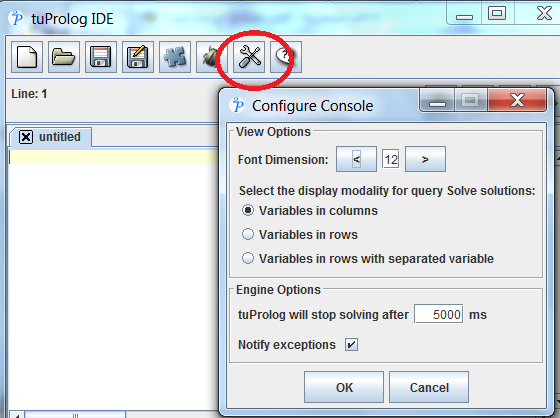
\includegraphics[width=7cm]{images/gui-config}
\caption{The configuration window.}
\label{fig:gui-configuration}
\end{figure}

%------------------------------------------------------
\subsection{Input from console}
\label{ssec:input-from-console}
%------------------------------------------------------

Until \tuprolog{} 2.7.x, an input from the standard input stream (e.g. via some of the IOLibrary/ISOIOLibrary input predicates, like \texttt{read}), could only be performed in the CUIConsole: any attempt to perform keyboard reading on the GUIConsole led to exception, because the underlying \emph{stdin} was uncaptured by the Prolog GUI.
This behaviour has been fixed in \tuprolog{} 2.8: henceforth, if a query performs a read operation from the standard input stream, the GUIConsole intercepts the request and shows the corresponding dialog (Figure \ref{fig:gui-InputFromConsole}). More on this in Section \ref{sec:io-library}.

\begin{figure}
\centering
  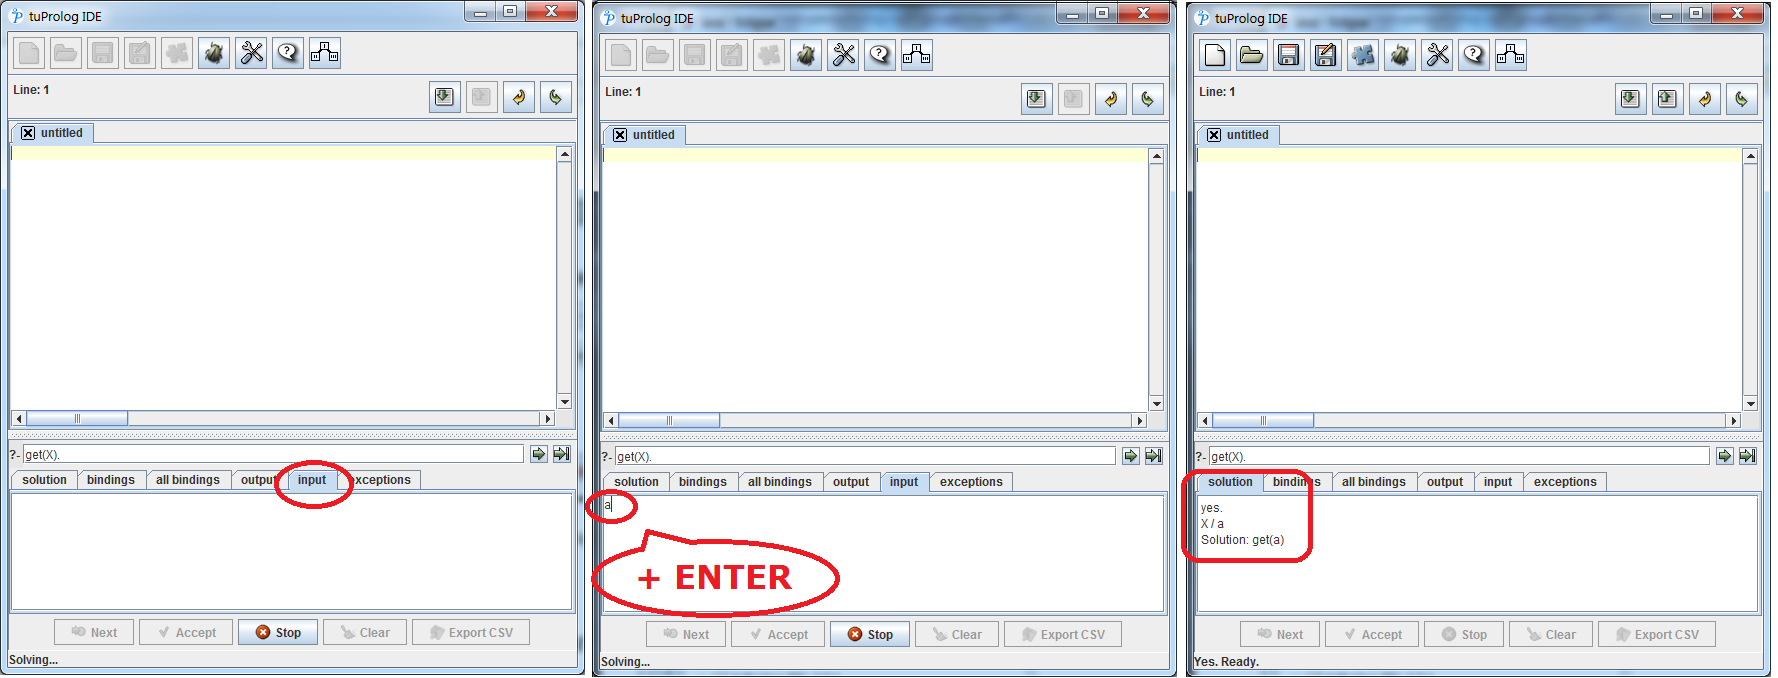
\includegraphics[width=7cm]{images/gui-InputFromConsole.png}
  \caption{Keyboard input management in the case of a read operation from the standard input.}\label{fig:gui-InputFromConsole}
\end{figure}

%=======================================================================
\section{\tuprolog{} for the Java Developer}
\label{sec:java-user-perspective}
%=======================================================================

As anticipated above, the Java developer can include \tuprolog{} in any of his projects, exploiting the \tuprolog{} API to access the Prolog engine(s) from his/her Java program: in fact, if your goal is just to embed intelligence in your Java application, all you need is adding the \texttt{tuprolog.jar} library (or the \texttt{2p.jar} library in the case you need also the extra classes) to your Java project, and develop normally---\tuprolog{} will be seen as any other referenced JAR archive.

However, if your goal is to develop a hybrid Java+Prolog application to be run from the Prolog side -- that is, where Java objects and methods are called from a Prolog program -- the \tuprolog{} plugin for Eclipse is probably the best choice, since it adds a specific \textit{tuprolog perspective} specifically suited for the needs of the Java/Prolog user (Figure \ref{fig:tuprologPluginGUI}).

\begin{figure}
\centering
  \includegraphics[width=300px]{images/tuprologPluginGUI.png}
  \caption{The \tuprolog{} plugin GUI for Eclipse.}\label{fig:tuprologPluginGUI}
\end{figure}

This perspective is mainly designed to support the development of multi-language, multi-paradigm applications (see Chapters \ref{ch:mpp-in-java}, \ref{ch:mpp-in-dotnet}), but can also be used as a standard Prolog console, writing (or loading) the Prolog theory in the editor and writing the query in the proper textfield---although the direct use of the \tuprolog{} GUI is probably faster for this purpose.

To use \tuprolog{} in Eclipse, one first needs to create a new \tuprolog{} project, and add a new theory file (\texttt{*.pl}) to the project.
%
To this end:%, three procedures are possible:
\begin{itemize}
  \item either select \texttt{New $>$ Project} from the Package Explorer's context menu, then select the \texttt{tuProlog} item;
  \item or, select \texttt{File $>$ New $>$ Other $>$ tuProlog $>$ tuProlog Project} from the main menu;
  \item or, press the \textit{New tuProlog Project} buttons in the \tuprolog{} toolbar (Figure \ref{fig:plugin1}.
\end{itemize}

In any case, a dialog appears (Figure \ref{fig:plugin2}) which prompts for the project name (default: \texttt{My\_Prolog\_Project}) and the desired Prolog libraries (the default set is proposed).

\begin{figure}
\centering
  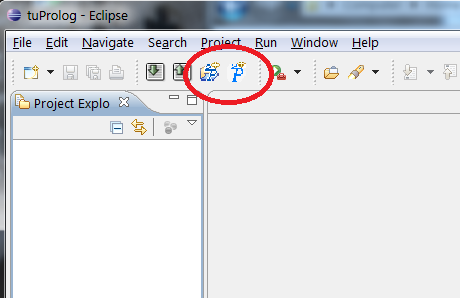
\includegraphics[width=200px]{images/plugin1.png}
  \caption{The \tuprolog{} toolbar}\label{fig:plugin1}
\end{figure}

\begin{figure}
\centering
  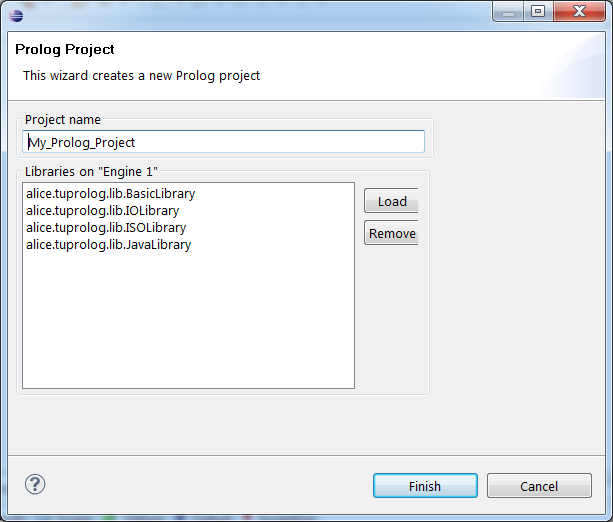
\includegraphics[width=200px]{images/plugin2.png}
  \caption{new \tuprolog{} project}\label{fig:plugin2}
\end{figure}

\begin{figure}
\centering
  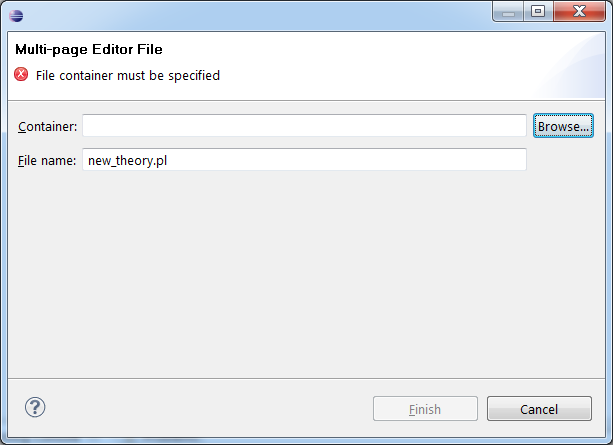
\includegraphics[width=200px]{images/plugin3.png}
  \caption{new \tuprolog{} file}\label{fig:plugin3}
\end{figure}

\begin{figure}
\centering
  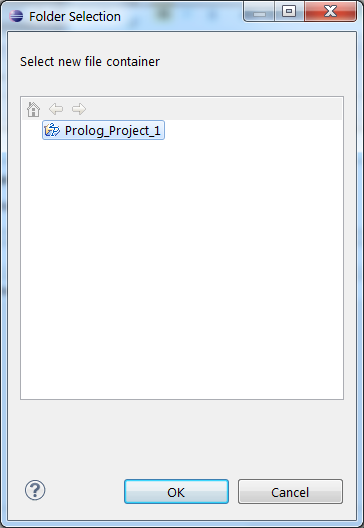
\includegraphics[width=200px]{images/plugin4.png}
  \caption{new \tuprolog{} file $>$ Browse...}\label{fig:plugin4}
\end{figure}

\begin{figure}
\centering
  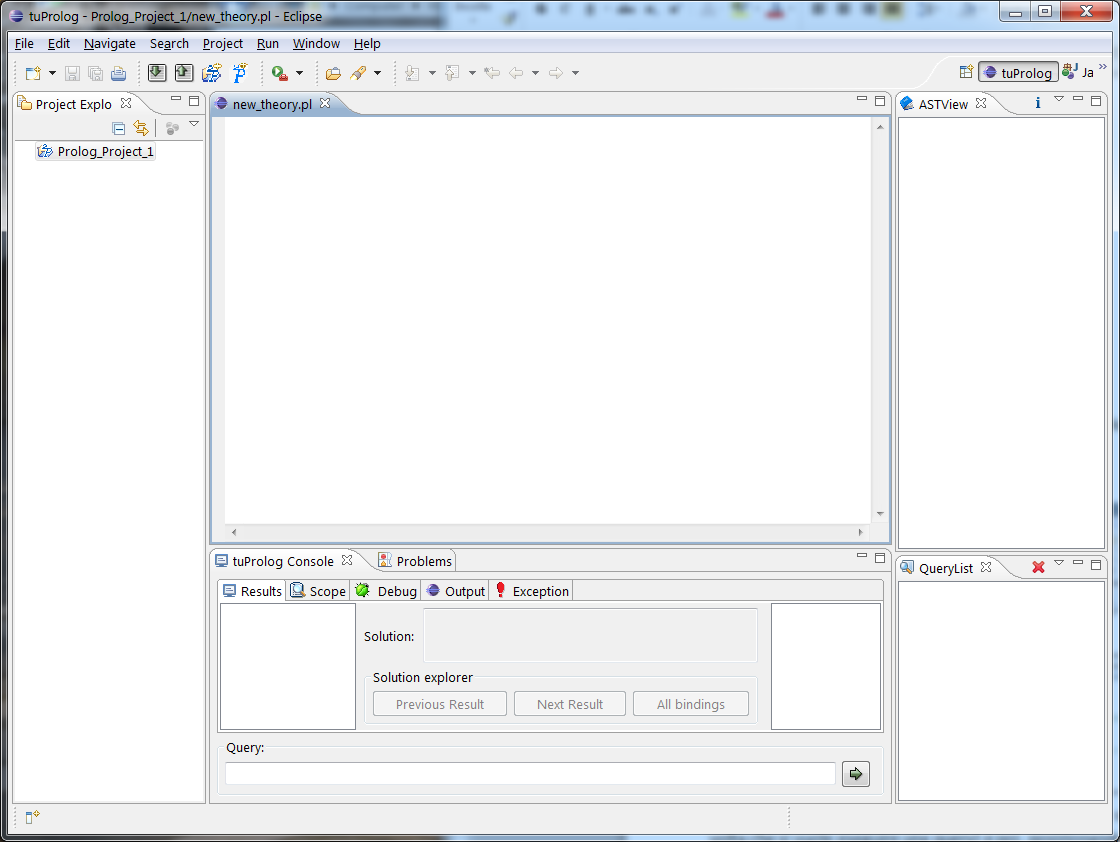
\includegraphics[width=200px]{images/plugin5.png}
  \caption{the \tuprolog{} perspective}\label{fig:plugin5}
\end{figure}

\begin{figure}
\centering
  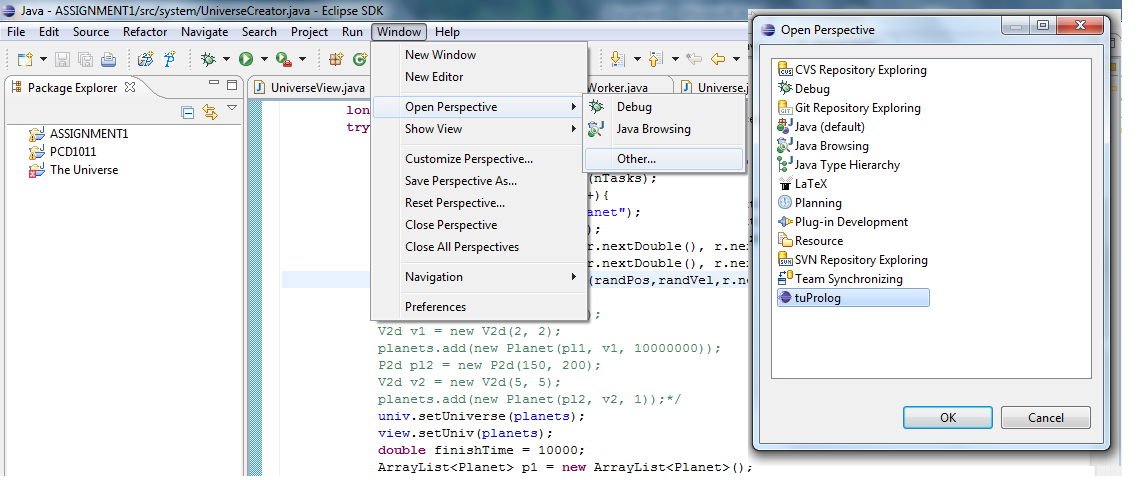
\includegraphics[width=200px]{images/plugin6.png}
  \caption{opening the \tuprolog{} perspective}\label{fig:plugin6}
\end{figure}

Pressing the \textit{New tuProlog File} button, a dialog appears which asks for the theory name (default: \texttt{new\_theory.pl}) and the file container, i.e. the tuProlog project where the new file has to be added (Figure \ref{fig:plugin3}); this is a mandatory argument. Pressing the \textit{Browse..} button, a new dialog proposes the current \tuprolog{} projects (Figure \ref{fig:plugin4}); again, the same result can be achieved via menu selection  (\texttt{File $>$ New $>$ Other $>$ tuProlog $>$ tuProlog Theory}). After confirming, the \tuprolog{} perspective automatically opens (Figure \ref{fig:plugin5}). Again, the same result can be achieved via the \texttt{Window $>$ Open Perspective} menu (Figure \ref{fig:plugin6}).

Once the theory has been written (or loaded), the theory file must be saved, either clicking the save icon in the toolbar, or choosing the \texttt{File $>$ Save} option, or hitting CTRL+S on the keyboard; this is mandatory before issuing any query.
The query can be written in the bottom console, and is executed either by pressing the Enter key, or by clicking the \textit{Solve} button.


\begin{figure}
\centering
  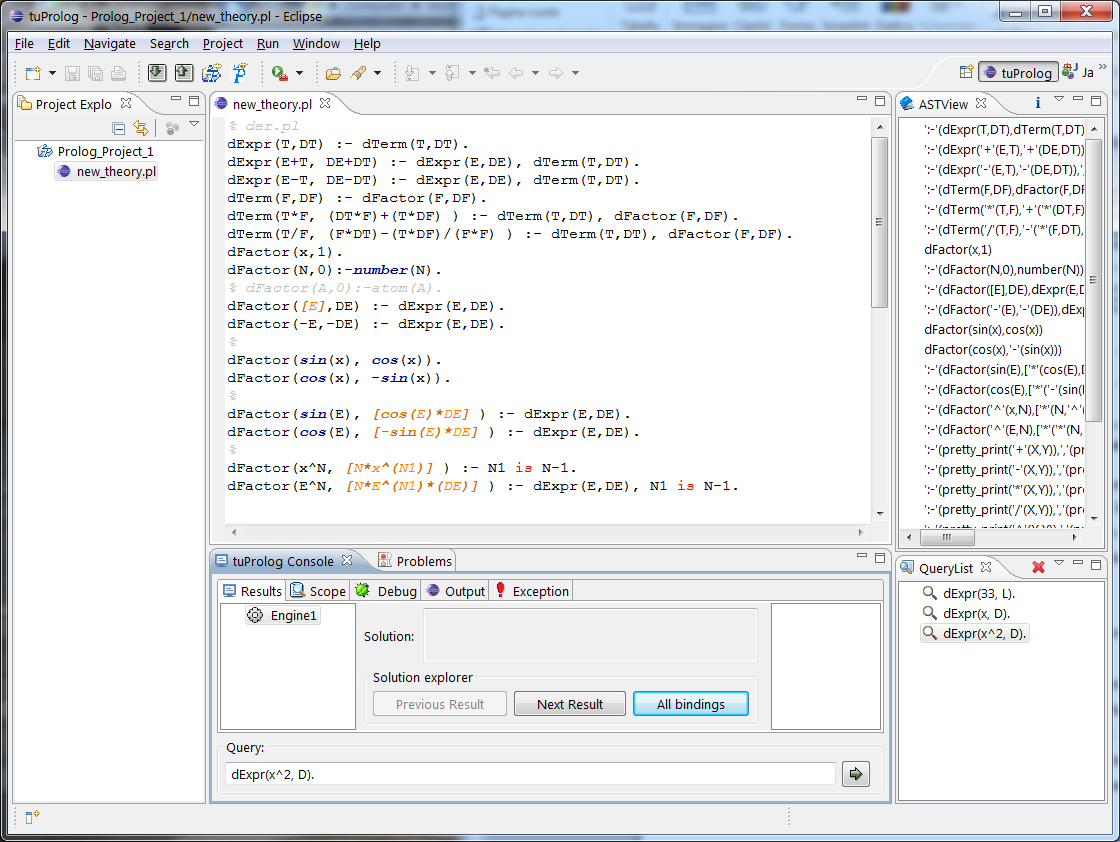
\includegraphics[width=4cm]{images/plugin7.png}
  \caption{executing queries, available views}\label{fig:plugin7}
\end{figure}

\begin{figure}
\centering
  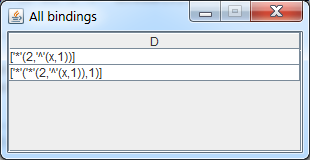
\includegraphics[width=200px]{images/plugin8.png}
  \caption{all variable bindings}\label{fig:plugin8}
\end{figure}

\begin{figure}
\centering
  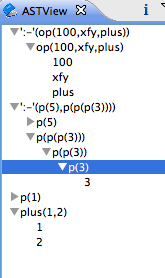
\includegraphics[width=200px]{images/plugin9.png}
  \caption{AST view (expanded)}\label{fig:plugin9}
\end{figure}

\begin{figure}
\centering
  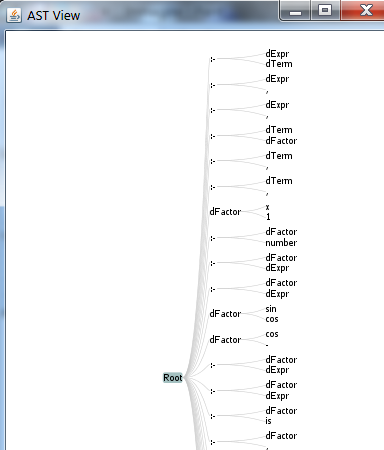
\includegraphics[width=200px]{images/plugin10.png}
  \caption{AST view (big term, expanded)}\label{fig:plugin10}
\end{figure}

The query results are shown in different views (Figure \ref{fig:plugin7}):
\begin{itemize}
  \item the \tuprolog{} Console view reports the query results: the variable bindings are also available pressing the \textit{All bindings} button (Figure \ref{fig:plugin8}).
  \item the Output view shows the program output messages;
  \item the QueryList view on the left side reports the list of all he executed queries, which can then be re-selected and re-executed in a click;
  \item the AST view shows the (dynamic) set of current clauses: pressing the \texttt{i} icon, a graphical view of the Abstract Syntax Tree produced by the Prolog parser is shown (Figures \ref{fig:plugin9} and \ref{fig:plugin10}).
\end{itemize}

It is worth highlighting that multiple \tuprolog{}  engines can be handled simultaneously: each engine can be selectively loaded with each own set of libraries and theories, and can be separately queried.
%
Moreover, in case of undeclared terms, a direct warning is issued in the plugin editor  (Figure \ref{fig:plugin11}).

\begin{figure}
\centering
  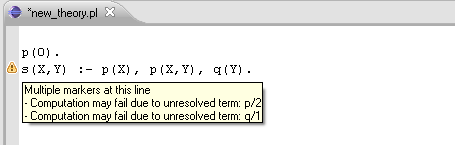
\includegraphics[width=200px]{images/plugin11.png}
  \caption{warning for undeclared terms}\label{fig:plugin11}
\end{figure}

%=======================================================================
\section{\tuprolog{} for the .NET Developer}
\label{sec:dotnet-user-perspective}
%=======================================================================

Since \tuprolog{}.NET is the result of an automatic conversion of the Java bytecode via IKVM \cite{ikvm}, everything in the Prolog user experience is identical whether the .NET or the Java GUI is used (see Section \ref{sec:prolog-user-perspective} above).

The .NET developer, however, can exploit \tuprolog{} in a .NET project, accessing its API from a program written in potentially any language available in the .NET platform.
%
Since no plugin is available for the de-facto standard tool used by most .NET programmers (i.e., Microsoft Visual Studio), there is no immediate way to see \tuprolog{} at work from within Visual Studio; however, the \tuprolog{} libraries can be easily added as external references for exploiting the available APIs, as one would do with any other library or third-party software.

For specific information about multi-paradigm programming in the context of the .NET platform, please refer to Chapter \ref{ch:mpp-in-dotnet}.


%=======================================================================
\section{\tuprolog{} for the Android User}
\label{sec:android-user-perspective}
%=======================================================================

Since \tuprolog{} is written in Java, the Java-Android developer wishing to include \tuprolog{} in an Android project can proceed very similarly to the Java developer, adding \texttt{tuprolog.jar} to the project libraries---though no plugin is available for this platform.

The Prolog-Android user, instead, can take advantage of the \tuprolog{} app, which shares the same core and libraries as the standard Java version, the only difference being the redesigned GUI--with special regard to the interaction with the file system.

Upon the application loading, the splash screen appears, immediately followed in a few seconds by the \textit{Home Activity} (Figure \ref{fig:android12}, left).
%
At the top, the name of the selected theory is reported (none at the beginning); below is the query textfield.
%
Four buttons enable the user to execute a query, ask for the next solution (when applicable), show the current solution and view the output console.
%
The menu button triggers the pop-up shown in Figure \ref{fig:android12} (right), whose main feature is \textit{List Theories}.

\begin{figure}
\centering
  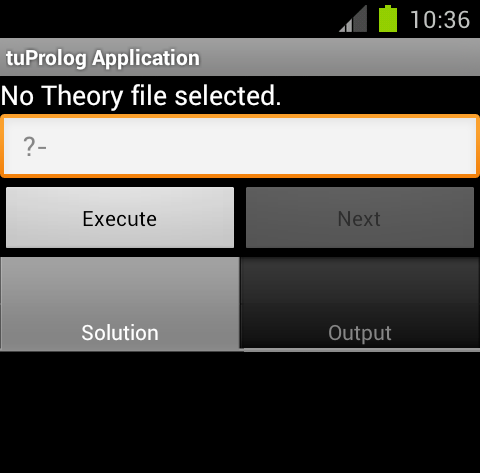
\includegraphics[width=200px]{images/android1.png}
  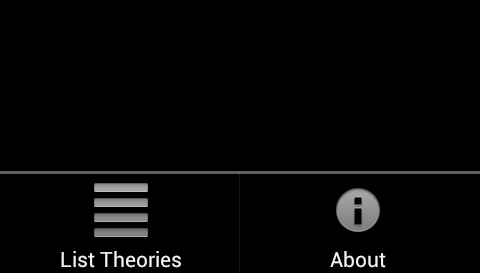
\includegraphics[width=200px]{images/android2.png}
  \caption{Home Activity (left) and its pop-up menu (right).}\label{fig:android12}
\end{figure}

Indeed, in \tuprolog{} for Android theories are not loaded directly in the Prolog engine from the file system, as in the standard Java version: rather, following Android recommendations, a \textit{theory database} mediator is provided, so as to separate the loading of a theory from its validity check---the latter being performed only when the theory is actually selected for being loaded into the engine. In this way, invalid theories (possibly incomplete, work-in-progress theories) can seamlessly be stored in the theory database, independently of their invalid nature.

So, theories of interest must be first loaded into the theory database (Figure \ref{fig:android34}, left): then, the theory to be actually loaded will be selected from such theories.
%
More precisely, to add a theory to the database, the menu option \textit{Import Theory to Database} is provided (Figure \ref{fig:android34}, right): a new activity opens that lets you browser the device's file system (Figure \ref{fig:android56}, left). Only the files that can be actually selected for addition to the theory database are shown: after a theory is successfully imported, the activity remembers the path for the next time, so as to make it faster to import multiple files.

\begin{figure}
\centering
  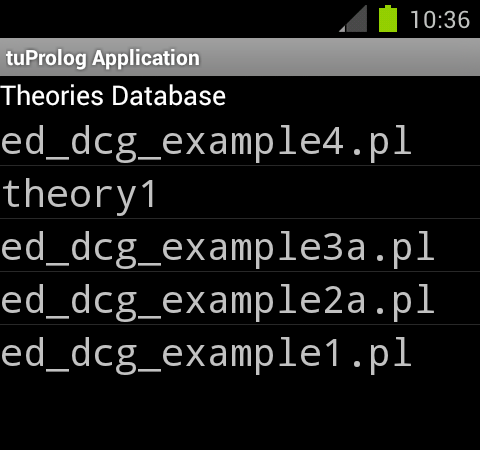
\includegraphics[width=150px]{images/android3.png}
  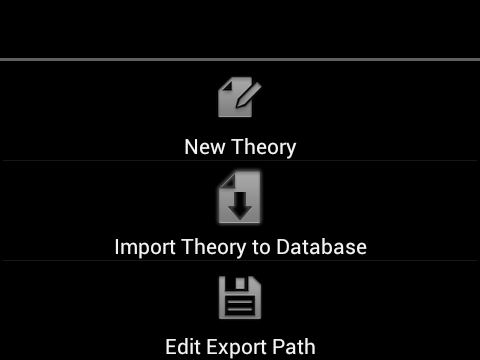
\includegraphics[width=150px]{images/android4.png}
  \caption{Theory database (left) and context menu (right)}\label{fig:android34}
\end{figure}

\begin{figure}
\centering
  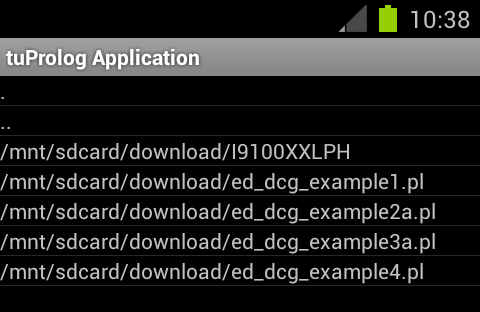
\includegraphics[width=150px]{images/android6.png}
  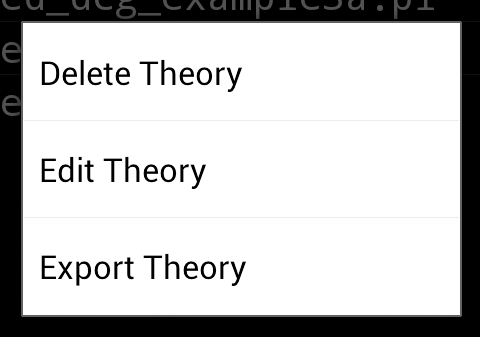
\includegraphics[width=150px]{images/android5.png}
  \caption{Browsing theories (left) and theory operations (right)}\label{fig:android56}
\end{figure}

\begin{figure}
\centering
  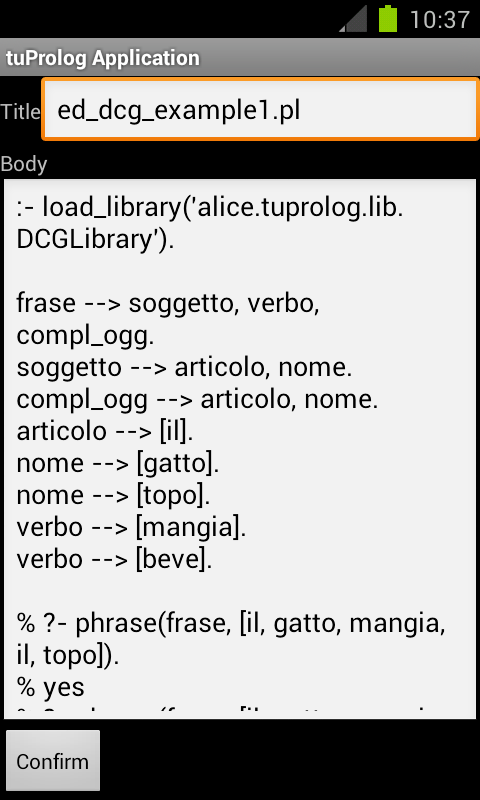
\includegraphics[width=150px]{images/android7.png}
  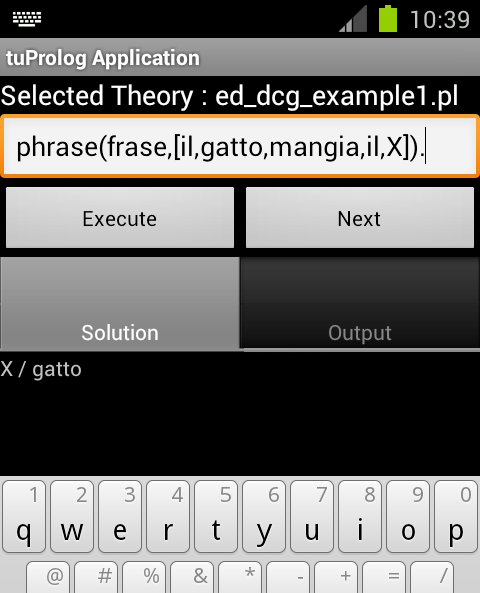
\includegraphics[width=150px]{images/android8.png}
  \caption{Theory editing (left) and query execution (right)}\label{fig:android78}
\end{figure}

Theories in the database can be deleted, edited and exported in a (long-)click, using the proper the context menu item (Figure \ref{fig:android56}, right). The export path can be changed via the \textit{Edit Export Path} in the activity menu.

Editing (Figure \ref{fig:android78}, left) applies both to existing (loaded) files and to brand new theories: to create a new theory, just click on \textit{New Theory} option in the context menu.
%
After editing, to make your changes permanent, the modified theory must be saved to the theory database by clicking the \textit{Confirm} button: alternatively, the back button discards changes.

When a valid theory is loaded, a query can be written in the input field (Figure \ref{fig:android78}, right): an auto-complete mechanism is available which exploits the previous queries to speed up the typing process.
%
Pressing \textit{Execute}, the query solution is shown in the \textit{Solution} tab, along with variable bindings; any output performed by the application is available in the \textit{Output} tab. If multiple solutions exist, the \textit{Next} button is enabled and can be exploited to browse them---the corresponding output being shown in the \textit{Output} tab.

Finally, if the query performs an operation requiring an input from the standard input stream (e.g. via some of the IOLibrary/ISOIOLibrary input predicates, like \texttt{read}), the app intercepts the request and shows the corresponding dialog (Figure \ref{fig:android9}): this feature is available since \tuprolog{} 2.8.
More on this in Section \ref{sec:io-library}.

\begin{figure}
\centering
  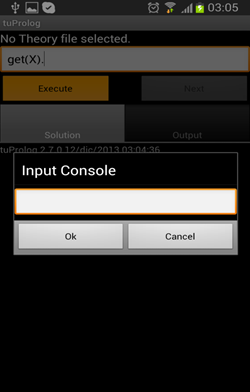
\includegraphics[width=150px]{images/android-inputFromConsole.png}
  \caption{Keyboard input management in the case of a read operation from the standard input.}\label{fig:android9}
\end{figure}

%******************************************************************************%
%=======================================================================
\chapter{\tuprolog{} Basics}
\label{ch:engine}
%=======================================================================

This chapter overviews the basic elements and structure of the \tuprolog{} engine, the \tuprolog{} syntax, the programming support, and the built-in predicates.
%
Additional predicates, provided by libraries, are presented in the next Chapter.

%---------------------------------------------------------------------
\section{Predicate categories}
\label{sec:predicate-categories}
%---------------------------------------------------------------------

In \tuprolog{}, predicates are organized into three different categories:
%
\begin{description}
\item[built-in predicates] |
Built-in predicates are so-called because they are defined at the \tuprolog{} core level. They constitute a small but essential set of predicates, that any \tuprolog{} engine can count on.
%
Any modification possibly made to the engine before or during execution will never affect the number and properties of these predicates.


\item[library predicates] |
Predicates loaded in a \tuprolog{} engine by means of a \tuprolog{} library are called library predicates.
%
Since libraries can be loaded and unloaded in \tuprolog{} engines freely at the system start-up, or dynamically at run time, the set of the library predicates of a \tuprolog{} engine is not fixed, and can change from engine to engine, as well as at different times for the same engine.
%
It is worth noting that library predicates cannot be individually retracted: to remove an undesired library predicate from the engine, the whole library containing that predicate needs to be unloaded.
%
%As discussed in Chapter \ref{ch:howto-develop-libraries}, \tuprolog{} libraries can be implemented mixing Java and Prolog code.

Library predicates can be overridden by theory predicates, that is, predicates defined in the user theory.


\item[theory predicates] |
Predicates loaded in a \tuprolog{} engine by means of a \tuprolog{} theory are called theory predicates.
%
Since theories can be loaded and unloaded in \tuprolog{} engines freely at the system start-up, or dynamically at execution time, the set of the theory predicates of a \tuprolog{} engine is not fixed, and can change from engine to engine, as well as at different times for the same engine.
%
%\tuprolog{} theories are collections of Prolog clauses.
\end{description}


It is worth highlighting that, though they may seem similar, library and theory predicates are not the same, and are handled differently by the \tuprolog{} engine.
%
The difference between the two categories is both \textit{conceptual} and \textit{structural}.

Conceptually speaking, theory predicates should be used to axiomatically represent domain knowledge at the time the proof is performed, while library predicates should be used to represent what is required (procedural knowledge, utility predicates) in order to actually and effectively perform proofs in the domain of interest. So, from this viewpoint, library predicates are devoted to represent more ``stable'' knowledge than theory predicates.
%
Correspondingly, library and theory predicates are represented differently at run-time, and are handled differently by the engine---in particular, with respect to the observation level for monitoring and debugging purposes.
%
In particular, library predicates are usually step over during debugging, coherently with their more stable (and expectedly well-tested) nature, while theory predicates are step into in a detailed way during the controlled execution.
%
This is also why all the tools in the \tuprolog{} GUI show in a separate way the theory predicates, on the one hand, and the loaded libraries and predicates, on the other.


%---------------------------------------------------------------------
\section{Syntax}
\label{sec:syntax}
%---------------------------------------------------------------------

The term syntax supported by \tuprolog{} engine is basically ISO compliant,\footnote{Some ISO directives, however, are not supported.} and accounts for several elements:
%
\begin{description}

\item[Atoms] |
There are four types of atoms:
\emph{(i)} a series of letters, digit, and/or underscores, beginning with a lower-case letter; \emph{(ii)} a series of one or more characters from the set \{\texttt{\#}, \texttt{\$}, \texttt{\&}, \texttt{*}, \texttt{+}, \texttt{-}, \texttt{.}, \texttt{/}, \texttt{:}, \texttt{<}, \texttt{=}, \texttt{>}, \texttt{?}, \texttt{@}, \texttt{\textasciicircum}, \texttt{\~}\}, provided it does not begin with \texttt{/*};
\emph{(iii)} The special atoms \texttt{[]} and \texttt{\{\}};
\emph{(iv)} a single-quoted string.

\item[Variables] |
A variable name begins with a capital
letter or the underscore mark (\bt{\_}), and consists of letters,
digits, and/or underscores.
%
A single underscore mark denotes an anonymous variable.

\item[Numbers] |
Integers and float are supported.
%
The formats supported for integer numbers are decimal, binary (with \verb|0b|
prefix), octal (with \verb|0o| prefix), and hexadecimal (with \verb|0x|
prefix). The character code format for integer numbers (prefixed by \verb|0'|) is supported only for alphanumeric characters, the white space, and characters in the set \{\texttt{\#}, \texttt{\$}, \texttt{\&}, \texttt{*}, \texttt{+}, \texttt{-}, \texttt{.}, \texttt{/}, \texttt{:}, \texttt{<}, \texttt{=}, \texttt{>}, \texttt{?}, \texttt{@}, \texttt{\textasciicircum}, \texttt{\~}\}.
%
The range of integers is -2147483648 to 2147483647; the range of floats is
-2E+63 to 2E+63-1.
%
Floating point numbers can be expressed also in the exponential format (e.g. \bt{-3.03E-05}, \bt{0.303E+13}).
%
A minus can be written before any number to make it negative (e.g. \bt{-3.03}).
%
Notice that the minus is the sign-part of the number itself; hence \bt{-3.4} is a number, not an expression (by contrast, \bt{- 3.4} is an expression).

\item[Strings] |
A series of ASCII characters, embedded in quotes \verb|'| or \verb|"|.
%
Within single quotes, a single quote is written double (e.g, \verb|'don''t forget'|).
%
A backslash at the very end of the line denotes continuation to the next line, so that: \\
\verb|'this is \ |\\
\verb|a single line'|\\
is equivalent to \verb|'this is a single line'| (the line break is ignored).
%
Within a string, the backslash can be used to denote special characters, such as \verb|\n| for a newline,
\verb|\r| for a return without newline,
\verb|\t| for a tab character,
\verb|\\| for a backslash,
\verb|\'| for a single quote,
\verb|\"| for a double quote.

\item[Compounds] |
The ordinary way to write a compound is to write the functor (as an atom), an opening parenthesis, without spaces between them, and then a series of terms separated by commas, and a closing parenthesis: \bt{f(a,b,c)}.
%
This notation can be used also for functors that are normally written as operators, e.g. \bt{2+2} = \verb|'+'(2,2)|.
%
Lists are defined as rightward-nested structures using the dot operator \verb|'.'|; so, for example: \\
\bt{[a] =} \verb|'.'(a,[])|\\
\bt{[a,b] =} \verb|'.'(a,'.'(b,[]))|\\
\bt{[a,b|c] =} \verb|'.'(a,'.'(b,c))|\\
%
There can be only one \bt{|} in a list, and no commas after it.
%
Also curly brackets are supported: any term enclosed with \bt{$\{$} and \bt{$\}$} is treated as the argument of the special functor \verb|'{}'|:  \verb|{hotel}| = \verb|'{}'(hotel)|, \bt{$\{$1,2,3$\}$} = \verb|'{}'(1,2,3)|.
%
Curly brackets can be used in the Definite Clause Grammars theory.


\item[Comments and Whitespaces] -- Whitespaces consist of blanks (including tabs and formfeeds), end-of-line marks, and comments. A whitespace can be put before and after any term, operator, bracket, or argument separator, as long as it does not break up an atom or number or separate a functor from the opening parenthesis that introduces its argument lists.
%
For instance, atom \bt{p(a,b,c)} can be written as \bt{p(\mbox{~a~},\mbox{~b~},\mbox{~c~})}, but not as \bt{\mbox{p~}(a,b,c)}).
%
Two types of comments are supported: one type begins with \bt{/*} and ends with \bt{*/}, the other begins with \bt{\%} and ends at the end of the line.
%
Nested comments are not allowed.


\item[Operators] |
Operators are characterised by a name, a specifier, and a priority.
%
An operator name is an atom, which is not univocal: the same atom can be an operator in more than one class, as in the case of the infix and prefix minus signs.
%
An operator  specifier is a string like \texttt{xfy}, which gives both its class (infix, postfix and prefix) and its associativity: \texttt{xfy} specifies that the grouping on the right should be formed first, \texttt{yfx} on the left, \texttt{xfx} no priority.
%
An operator priority is a non-negative integer ranging from 0 (max priority) and 1200 (min priority).

Operators can be defined by means of either the \bt{op/3} predicate or directive.
%
No predefined operators are directly given by the raw \tuprolog{} engine, whereas a number of them is provided through libraries.

\item[Commas] |
The comma has three functions: it separates arguments of functors, it separates elements of lists, and it is an infix operator of priority 1000.
%
Thus \bt{(a,b)} (without a functor in front) is a compound, equivalent to \verb|','(a,b)|.

\item[Parentheses] -- Parentheses are allowed around any term.
%
The effect of parentheses is to override any grouping that may
otherwise be imposed by operator priorities.
%
Operators enclosed in parentheses do not work as operators;
thus \bt{2(+)3} is a syntax error.
\end{description}

%---------------------------------------------------------------------
\section{Engine configurability}
\label{sec:engine-configurability}
%---------------------------------------------------------------------
\tuprolog{} engines provides four levels of configurability:

\begin{description}

\item[Libraries] |
At the first level, each \tuprolog{} engine can be dynamically extended by loading or unloading libraries.
%
Each library can provide a specific set of predicates, functors, and a related theory, which also allows new flags and operators to be defined.
%
Libraries can be either pre-defined (see Chapter \ref{ch:standard-libraries}) or user-defined (see Section \ref{sec:howto-develop-libraries}).
%
A library can be loaded by means of the predicate \texttt{load\_library} (Prolog side), or by means of the method \texttt{loadLibrary} of the \tuprolog{} engine (Java/.NET side).


\item[Directives] |
At the second level, directives can be given by means of the \bt{:-/1} predicate, which is natively supported by the engine, and can be used to configure and use a \tuprolog{} engine (\bt{set\_prolog\_flag/1}, \bt{load\_library/1}, \bt{consult/1}, \bt{solve/1}), format and syntax of read-terms\footnote{As specified by the ISO standard, a read-term is a Prolog term followed by an end token, composed by an optional layout text sequence and a dot.} (\bt{op/3}).
%
Directives are described in detail in the following sections.

\item[Flags] |
At the third level, \tuprolog{} supports the dynamic definition of flags to describe relevant aspects of libraries, predicates and evaluable functors.
%
A flag is identified by a name (an alphanumeric atom), a list of possible values, a default value, and a boolean value specifying if the flag value can be modified.
%
Dynamically, a flag value can be changed (if modifiable) with a new value included in the list of possible values.

\item[Theories] |
The fourth level of configurability is given by theories: a theory is a text consisting of a sequence of clauses and/or directives.
%
Clauses and directives are terminated by a dot, and are separated by a whitespace character.
%
Theories can be loaded or unloaded by means of suitable library predicates, which are described in Chapter \ref{ch:standard-libraries}.

\end{description}

%---------------------------------------------------------------------
\section{Exception support}
\label{sec:exception-support}
%---------------------------------------------------------------------

As of version 2.2, \tuprolog{} supports exceptions according to the ISO Prolog standard (ISO/IEC 13211-1) published in 1995.
%
Details about the exception handling mechanism are provided in Chapter \ref{ch:exceptions}: this short overview is functional to the understanding of the built-in predicate specification presented in the next Section.

According to the ISO specification, an \textit{error} is a particular circumstance that interrupts the execution of a Prolog program: when a Prolog engine encounters an error, it raises an \textit{exception}, which is supposed to transfer the execution flow to a suitable exception handler, exiting atomically from any number of nested execution contexts.

%-----------------------------------------------------------------------
\subsection{Error classification}
\label{ssec:error classification}
%-----------------------------------------------------------------------
When an exception is raised, the relevant error information is also transferred by instantiating a suitable \textit{error term}.

The ISO Prolog standard prescribes that such a term follows the pattern
\texttt{error(\textit{Error\_term}, \textit{Implementation\_defined\_term})} where
\texttt{\textit{Error\_term}} is constrained by the standard to a pre-defined set of values (the error categories), and \texttt{\textit{Implementation\_defined\_term}} is an optional term providing implementation-specific details.
%
Ten error categories are defined:
\begin{enumerate}
  \item \texttt{instantiation\_error}: when the argument of a predicate or one of its components is an unbound variable, which should have been instantiated. Example: \texttt{X is Y+1} when \texttt{Y} is not instantiated at the time \texttt{is/2} is evaluated.

  \item \texttt{type\_error(\textit{ValidType}, \textit{Culprit})}: when the type of an argument of a predicate, or one of its components, is instantiated, but is bound to the wrong type of data. \texttt{\textit{ValidType}} represents the expected data type (one of \texttt{atom}, \texttt{atomic}, \texttt{byte}, \texttt{callable}, \texttt{character}, \texttt{evaluable}, \texttt{in\_byte}, \texttt{in\_character}, \texttt{integer}, \texttt{list}, \texttt{number}, \texttt{predicate\_indicator}, \texttt{variable}), and \texttt{\textit{Culprit}} is the actual (wrong) type found.
      Example: a predicate expecting months to be represented as integers in the range 1--12 called with an argument like \texttt{march} instead of \texttt{3}.

  \item \texttt{domain\_error(\textit{ValidDomain}, \textit{Culprit})}: when the argument type is correct, but its value falls outside the expected range.
      \texttt{\textit{ValidDomain}} is one of \texttt{character\_code\_list},
      \texttt{not\_empty\_list}, \texttt{not\_less\_than\_zero}, \texttt{close\_option}, \texttt{io\_mode}, \texttt{operator\_priority}, \texttt{operator\_specifier}, \texttt{flag\_value}, \texttt{prolog\_flag}, \texttt{read\_option}, \texttt{write\_option}, \texttt{source\_sink}, \texttt{stream}, \texttt{stream\_option}, \texttt{stream\_or\_alias}, \texttt{stream\_position},\\
      \texttt{stream\_property}. Example: a predicate expecting months as above, called with an out-of-range argument like \texttt{13}.

  \item \texttt{existence\_error(\textit{ObjectType}, \textit{ObjectName}}): when the referenced object does not exist. \texttt{\textit{ObjectType}} is
      the type of the unexisting object (one of \texttt{procedure}, \texttt{source\_sink}, or \texttt{stream}), and \texttt{\textit{ObjectName}} is the missing object's name. Example: trying to access an unexisting file like \texttt{usr/goofy} leads to an
      \texttt{existence\_error(stream, 'usr/goofy')}.

  \item \texttt{permission\_error(\textit{Operation}, \textit{ObjectType}, \textit{Object})}: whenever\\
       \texttt{\textit{Operation}} (one of \texttt{access}, \texttt{create}, \texttt{input}, \texttt{modify}, \texttt{open}, \texttt{output}, or \texttt{reposition}) is not allowed on \texttt{\textit{Object}}, of type \texttt{\textit{ObjectType}} (one of  \texttt{binary\_stream}, \texttt{past\_end\_of\_stream}, \texttt{operator}, \texttt{private\_procedure}, \texttt{static\_procedure}, \texttt{source\_sink}, \texttt{stream}, \texttt{text\_stream}, \texttt{flag}).

  \item \texttt{representation\_error(\textit{Flag})}: when an implementation-defined limit, whose category is given by \texttt{\textit{Flag}} (one of
      \texttt{character}, \texttt{character\_code}, \texttt{in\_character\_code}, \texttt{max\_arity}, \texttt{max\_integer}, \texttt{min\_integer}), is violated during execution.

  \item \texttt{evaluation\_error(\textit{Error})}: when the evaluation of a function produces an out-of-range value (one of \texttt{float\_overflow}, \texttt{int\_overflow}, \texttt{undefined}, \texttt{underflow}, \texttt{zero\_divisor}).

  \item \texttt{resource\_error(\textit{Resource})}: when the Prolog engine does not have enough resources to complete the execution of the goal. \texttt{Resource} can be any term useful to describe the situation. Examples: maximum number of opened files reached, no further available memory, etc.

  \item \texttt{syntax\_error(\textit{Message})}: when data read from an external source have an incorrect format or cannot be processed for some reason. \texttt{\textit{Message}} can be any term useful to describe the situation.

  \item \texttt{system\_error}: any other unexpected error not falling into the previous categories.
\end{enumerate}


%---------------------------------------------------------------------
\section{Built-in predicates}
\label{sec:builtins}
%---------------------------------------------------------------------

This section contains a comprehensive list of the built-in predicates, that is the predicated defined directly in the \tuprolog{} core, both for efficiency reasons and because they directly affect the resolution process.

Following an established convention, the symbol \bt{+} in front of an argument means an \emph{input argument}, \bt{-} means \emph{output argument}, \bt{?} means \emph{input/output} argument, \bt{@} means \emph{input argument} that must be bound.

%---------------------------------------------------------------------
\subsection{Control management}
\label{ssec:control-management}
%---------------------------------------------------------------------

\begin{itemize}

\item \bti{true/0}\\
    \noindent\bt{true} is true.

\item \bti{fail/0}\\
    \noindent\bt{fail} is false.

\item \verb|','/2|\\
    \noindent\verb|','(First,Second)| is true if and only if both \bt{First}
    and \bt{Second} are true.

\item \bti{!/0}\\
    \noindent\bt{!} is true. All choice points between the cut and the
    parent goal are removed. The effect is a commitment to use both the
    current clause and the substitutions found at the point of the
    cut.

\item \verb|'$call'/1|\\
    \noindent\verb|'$call'(Goal)| is true if and only if \bt{Goal}
    represents a true goal. It is not opaque to cut.

    \template{'\$call'(+callable\_term)}

    \exception{error(instantiation\_error, instantiation\_error(\\
    Goal, ArgNo))} when \texttt{G} is a variable. \texttt{Goal} is the goal where the problem occurred, \texttt{ArgNo} indicates the argument that caused the problem (obviously, \texttt{1}).

    \exception{error(type\_error(ValidType, Culprit), type\_error(\\
    Goal, ArgNo, ValidType, Culprit))} when \texttt{G} is not a callable goal. \texttt{Goal} is the goal where the problem occurred, \texttt{ArgNo} indicates the argument that caused the problem (obviously, \texttt{1}), \texttt{ValidType} is the data type expected for \texttt{G} (here, \texttt{callable}), while \texttt{Culprit} is the actual data type found.

\item \bti{halt/0}\\
    \noindent\bt{halt} terminates a Prolog demonstration, exiting the
    Prolog thread and returning to the parent system. In any of the \tuprolog{} user interfaces -- the GUI, the character-based console, the Android app, the Eclipse plugin -- the effect is to terminate the whole application (including Eclipse itself).

\item \bti{halt/1}\\
    \noindent\bt{halt(X)} terminates a Prolog demonstration, exiting the
    Prolog thread and returning the provided int value to the parent system.
    In any of the \tuprolog{} user interfaces -- the GUI, the character-based console, the Android app, the Eclipse plugin -- the effect is to terminate the whole application (including Eclipse itself).

    \template{halt(+int)}

    \exception{error(instantiation\_error, instantiation\_error(\\
    Goal, ArgNo))} when \texttt{X} is a variable. \texttt{Goal} is the goal where the problem occurred, \texttt{ArgNo} indicates the argument that caused the problem (obviously, \texttt{1}).

    \exception{error(type\_error(ValidType, Culprit), type\_error(\\
    Goal, ArgNo, ValidType, Culprit))} when \texttt{X} is not an integer number. \texttt{Goal} is the goal where the problem occurred, \texttt{ArgNo} indicates the argument that caused the problem (obviously, \texttt{1}), \texttt{ValidType} is the data type expected for \texttt{X} (here, \texttt{integer}), while \texttt{Culprit} is the actual data type found.

\end{itemize}

%---------------------------------------------------------------------
\subsection{Term unification and management}
\label{ssec:term-unification-and-management}
%---------------------------------------------------------------------

\begin{itemize}

\item \bti{is/2}\\
    \noindent\bt{is(X, Y)} is true iff \bt{X} is unifiable with the value of the expression \bt{Y}.

    \template{is(?term, @evaluable)}

    \exception{error(instantiation\_error, instantiation\_error(\\
    Goal, ArgNo))} when \texttt{Y} is a variable. \texttt{Goal} is the goal where the problem occurred, \texttt{ArgNo} indicates the argument that caused the problem (here, \texttt{2}).

    \exception{error(type\_error(ValidType, Culprit), type\_error(\\
    Goal, ArgNo, ValidType, Culprit))} when \texttt{Y} is not a valid expression. \texttt{Goal} is the goal where the problem occurred, \texttt{ArgNo} indicates the argument that caused the problem (clearly, \texttt{2}), \texttt{ValidType} is the data type expected for \texttt{G} (here, \texttt{evaluable}), while \texttt{Culprit} is the actual data type found.

    \exception{error(evaluation\_error (Error), evaluation\_error(\\
    Goal, ArgNo, Error))} when an error occurs during the evaluation of \texttt{Y}. \texttt{Goal} is the goal where the problem occurred, \texttt{ArgNo} indicates the argument that caused the problem (clearly, \texttt{2}), and \texttt{Error} is the error occurred (e.g. \texttt{zero\_division} in case of a division by zero).

\item \verb|'='/2|\\
    \noindent\verb|'='(X, Y)| is true iff \bt{X} and \bt{Y} are unifiable.

    \template{'='(?term, ?term)}

\item \verb|'\='/2|\\
    \noindent\verb|'\='(X, Y)| is true iff \bt{X} and \bt{Y} are not unifiable.

    \template{'$\setminus$='(?term, ?term)}

\item \verb|'$tolist'/2|\\
    \noindent\verb|'$tolist'(Compound, List)| is true if \bt{Compound} is a compound term, and in this case \bt{List} is list representation of the compound, with the name as first element and all the arguments as other elements.

    \template{'\$tolist'(@struct, -list)}

    \exception{error(instantiation\_error, instantiation\_error(\\
    Goal, ArgNo))} when \texttt{Struct} is a variable. \texttt{Goal} is the goal where the problem occurred, \texttt{ArgNo} indicates the argument that caused the problem (obviously, \texttt{1}).

    \exception{error(type\_error(ValidType, Culprit), type\_error(\\
    Goal, ArgNo, ValidType, Culprit))} when \texttt{Struct} is not a structure. \texttt{Goal} is the goal where the problem occurred, \texttt{ArgNo} indicates the argument that caused the problem (clearly, \texttt{1}), \texttt{ValidType} is the data type expected for \texttt{G} (here, \texttt{struct}), while \texttt{Culprit} is the actual data type found.

\item \verb|'$fromlist'/2|\\
    \noindent\verb|'$fromlist'(Compound, List)| is true if \bt{Compound} unifies with the list representation of \bt{List}.

    \template{'\$fromlist'(-struct, @list)}

    \exception{error(instantiation\_error, instantiation\_error(\\
    Goal, ArgNo))} when \texttt{List} is a variable. \texttt{Goal} is the goal where the problem occurred, \texttt{ArgNo} indicates the argument that caused the problem (obviously, \texttt{2}).

    \exception{error(type\_error(ValidType, Culprit), type\_error(\\
    Goal, ArgNo, ValidType, Culprit))} when \texttt{List} is not a list. \texttt{Goal} is the goal where the problem occurred, \texttt{ArgNo} indicates the argument that caused the problem (clearly, \texttt{2}), \texttt{ValidType} is the data type expected for \texttt{G} (here, \texttt{list}), while \texttt{Culprit} is the actual data type found.

\item \bti{copy\_term/2}\\
    \noindent\bt{copy\_term(Term1, Term2)} is true iff \bt{Term2} unifies with the a renamed copy of \bt{Term1}.

    \template{copy\_term(?term, ?term)}

\item \verb|'$append'/2|\\
    \noindent\verb|'$append'(Element, List)| is true if \bt{List} is a list, with the side effect that the \bt{Element} is appended to the list.

    \template{'\$append'(+term, @list)}

    \exception{error(instantiation\_error, instantiation\_error(\\
    Goal, ArgNo))} when \texttt{List} is a variable. \texttt{Goal} is the goal where the problem occurred, \texttt{ArgNo} indicates the argument that caused the problem (obviously, \texttt{2}).

    \exception{error(type\_error(ValidType, Culprit), type\_error(\\
    Goal, ArgNo, ValidType, Culprit))} when \texttt{List} is not a list. \texttt{Goal} is the goal where the problem occurred, \texttt{ArgNo} indicates the argument that caused the problem (clearly, \texttt{2}), \texttt{ValidType} is the data type expected for \texttt{G} (here, \texttt{list}), while \texttt{Culprit} is the actual data type found.

\end{itemize}

%---------------------------------------------------------------------
\subsection{Knowledge base management}
\label{ssec:knowledge-base-management}
%---------------------------------------------------------------------

\begin{itemize}

\item
    \verb|'$find'/2|\\
    \noindent\verb|'$find'(Clause, Clauses)| is true if \bt{Clause} is a clause and \bt{Clauses} is a list: as a side effect, all the database clauses matching \bt{Clause} are appended to the \bt{Clauses} list.

    \template{'\$find'(@clause, @list)}

    \exception{error(instantiation\_error, instantiation\_error(\\
    Goal, ArgNo))} when \texttt{Clause} is a variable. \texttt{Goal} is the goal where the problem occurred, \texttt{ArgNo} indicates the argument that caused the problem (here, \texttt{1}).

    \exception{error(type\_error(ValidType, Culprit), type\_error(\\
    Goal, ArgNo, ValidType, Culprit))} when \texttt{Clauses} is not a list. \texttt{Goal} is the goal where the problem occurred, \texttt{ArgNo} indicates the argument that caused the problem (here, \texttt{2}), \texttt{ValidType} is the data type expected for \texttt{Clauses} (i.e. \texttt{list}), while \texttt{Culprit} is the actual data type found.

\item
    \bti{abolish/1}\\
    \noindent\bt{abolish(Predicate)} completely wipes out the dynamic
    predicate matching \texttt{Predicate}.

    \template{\bt{abolish(@term)}}

    \exception{error(instantiation\_error, instantiation\_error(\\
    Goal, ArgNo))} when \texttt{Predicate} is a variable. \texttt{Goal} is the goal where the problem occurred, \texttt{ArgNo} indicates the argument that caused the problem (obviously, \texttt{1}).

    \exception{error(type\_error(ValidType, Culprit), type\_error(\\
    Goal, ArgNo, ValidType, Culprit))} when \texttt{Predicate} is not a structure. \texttt{Goal} is the goal where the problem occurred, \texttt{ArgNo} indicates the argument that caused the problem (obviously, \texttt{1}), \texttt{ValidType} is the data type expected for \texttt{Predicate}, while \texttt{Culprit} is the actual data type found.

\item \bti{asserta/1}\\
    \noindent\bt{asserta(Clause)} is true, with the side effect that
    the clause \bt{Clause} is added to the beginning of database.

    \template{asserta(@clause)}

    \exception{error(instantiation\_error, instantiation\_error(\\
    Goal, ArgNo))} when \texttt{Clause} is a variable. \texttt{Goal} is the goal where the problem occurred, \texttt{ArgNo} indicates the argument that caused the problem (obviously, \texttt{1}).

    \exception{error(type\_error(ValidType, Culprit), type\_error(\\
    Goal, ArgNo, ValidType, Culprit))} when \texttt{Clause} is not a structure. \texttt{Goal} is the goal where the problem occurred, \texttt{ArgNo} indicates the argument that caused the problem (obviously, \texttt{1}), \texttt{ValidType} is the data type expected for \texttt{Clause}, while \texttt{Culprit} is the actual data type found.

\item \bti{assertz/1}\\
    \noindent\bt{assertz(Clause)} is true, with the side effect that
    the clause \bt{Clause} is added to the end of the database.

    \template{assertz(@clause)}

    \exception{error(instantiation\_error, instantiation\_error(\\
    Goal, ArgNo))} when \texttt{Clause} is a variable. \texttt{Goal} is the goal where the problem occurred, \texttt{ArgNo} indicates the argument that caused the problem (obviously, \texttt{1}).

    \exception{error(type\_error(ValidType, Culprit), type\_error(\\
    Goal, ArgNo, ValidType, Culprit))} when \texttt{Clause} is not a structure. \texttt{Goal} is the goal where the problem occurred, \texttt{ArgNo} indicates the argument that caused the problem (obviously, \texttt{1}), \texttt{ValidType} is the data type expected for \texttt{Clause}, while \texttt{Culprit} is the actual data type found.

\item \verb|'$retract'/1|\\
    \noindent\verb|'$retract'(Clause)| is true if the database contains
    at least one clause unifying with \bt{Clause}; as a side effect, the
    clause is removed from the database. It is not re-executable.
    Please do not confuse this built-in predicate with the \texttt{retract/1} predicate of \textit{BasicLibrary}.

    \template{'\$retract'(@clause)}

    \exception{error(instantiation\_error, instantiation\_error(\\
    Goal, ArgNo))} when \texttt{Clause} is a variable. \texttt{Goal} is the goal where the problem occurred, \texttt{ArgNo} indicates the argument that caused the problem (obviously, \texttt{1}).

    \exception{error(type\_error(ValidType, Culprit), type\_error(\\
    Goal, ArgNo, ValidType, Culprit))} when \texttt{Clause} is not a structure. \texttt{Goal} is the goal where the problem occurred, \texttt{ArgNo} indicates the argument that caused the problem (obviously, \texttt{1}), \texttt{ValidType} is the data type expected for \texttt{Clause}, while \texttt{Culprit} is the actual data type found.

\end{itemize}

%---------------------------------------------------------------------
\subsection{Operator and flag management}
\label{ssec:operator-and-flag-management}
%---------------------------------------------------------------------

\begin{itemize}

\item \bti{op/3}\\
    \noindent\bt{op(Priority, Specifier, Operator)} is true. It always succeeds,
    modifying the operator table as a side effect. If \bt{Priority} is 0, then
    \bt{Operator} is removed from the operator table; else, \bt{Operator} is
    added to the operator table, with priority (lower binds tighter) \bt{Priority}
    and associativity determined by \bt{Specifier}. If an operator with the same
    \bt{Operator} symbol and the same \bt{Specifier} already exists in the operator
    table, the predicate modifies its priority according to the specified \bt{Priority} argument.

    \template{op(+integer, +specifier, @atom\_or\_atom\_list)}

 \item \bti{flag\_list/1}\\
     \noindent\bt{flag\_list(FlagList)} is true and \bt{FlagList} is the list of the flags currently defined in the engine.

     \template{flag\_list(-list)}

\item \bti{set\_prolog\_flag/2}\\
    \noindent\bt{set\_prolog\_flag(Flag, Value)} is true, and as a side effect associates \bt{Value} with the flag \bt{Flag}, where \bt{Value} is a value that is within the implementation defined range of values for \bt{Flag}.

    \template{set\_prolog\_flag(+flag, @nonvar)}

    \exception{error(instantiation\_error, instantiation\_error(\\
    Goal, ArgNo))} if either \texttt{Flag} or \texttt{Value} is a variable. \texttt{Goal} is the goal where the problem occurred, \texttt{ArgNo} indicates the argument that caused the problem (\texttt{1} or \texttt{2}).

    \exception{error(type\_error(ValidType, Culprit), type\_error(\\
    Goal, ArgNo, ValidType, Culprit))} if \texttt{Flag} is not a structure or \texttt{Value} is not ground. \texttt{Goal} is the goal where the problem occurred, \texttt{ArgNo} indicates the argument that caused the problem (\texttt{1} or \texttt{2}), \texttt{Valid-}\\\texttt{Type} is the data type expected for \texttt{Flag} or \texttt{Value} (\texttt{struct} or \texttt{ground}, respectively), while \texttt{Culprit} is the actual wrong term (either \texttt{Flag} or \texttt{Value}).

    \exception{error(domain\_error(ValidDomain, Culprit), domain\_\\error(Goal, ArgNo, ValidDomain, Culprit))} if \texttt{Flag} is undefined in the engine or \texttt{Value} is not admissible for \texttt{Flag}. \texttt{Goal} is the goal where the problem occurred, \texttt{ArgNo} indicates the argument that caused the problem (\texttt{1} or \texttt{2}), \texttt{ValidDomain} is the data type expected for \texttt{Flag} or \texttt{Value} (\texttt{prolog\_flag} or \texttt{flag\_value}, respectively), while \texttt{Culprit} is the actual wrong term (either \texttt{Flag} or \texttt{Value}).

    \exception{error(permission\_error(Operation, ObjectType,\\Culprit), permission\_error(Goal, Operation, ObjectType,\\Culprit, Message))} if \texttt{Flag} is unmodifiable. \texttt{Goal} is the goal where the problem occurred, \texttt{Operation} is the operation that caused the problem (\texttt{modify}), \texttt{ObjectType} is the data type of the flag (i.e. \texttt{flag}), \texttt{Culprit} is the actual wrong term (clearly, \texttt{Flag}), and \texttt{Message} adds possible extra info (by convention, the atom \texttt{0} is used when no extra info exists).

\item \bti{get\_prolog\_flag/2}\\
    \noindent\bt{get\_prolog\_flag(Flag, Value)} is true iff \bt{Flag} is a flag supported by the engine and \bt{Value} is the value currently associated with it. It is not re-executable.

    \template{get\_prolog\_flag(+flag, ?term)}

    \exception{error(instantiation\_error, instantiation\_error(\\
    Goal, ArgNo))} when \texttt{Flag} is a variable. \texttt{Goal} is the goal where the problem occurred, \texttt{ArgNo} indicates the argument that caused the problem (obviously, \texttt{1}).

    \exception{error(type\_error(ValidType, Culprit), type\_error(\\
    Goal, ArgNo, ValidType, Culprit))} when \texttt{Flag} is not a structure. \texttt{Goal} is the goal where the problem occurred, \texttt{ArgNo} indicates the argument that caused the problem (clearly, \texttt{1}), \texttt{ValidType} is the data type expected for \texttt{G} (here, \texttt{struct}), while \texttt{Culprit} is the actual data type found.

    \exception{error(domain\_error(ValidDomain, Culprit), domain\_\\error(Goal, ArgNo, ValidDomain, Culprit))} if \texttt{Flag} is undefined in the engine. \texttt{Goal} is the goal where the problem occurred, \texttt{ArgNo} indicates the argument that caused the problem (clearly, \texttt{1}), \texttt{ValidDomain} is the domain expected for \texttt{G} (here, \texttt{prolog\_flag}), while \texttt{Culprit} is the actual wrong term found.

\end{itemize}

%---------------------------------------------------------------------
\subsection{Library management}
\label{ssec:library-management}
%---------------------------------------------------------------------

\begin{itemize}

\item \bti{load\_library/1}\\
    \bt{load\_library(LibraryName)} is true if \bt{LibraryName} is the name of a \tuprolog{} library available for loading. As side effect, the specified library is loaded by the engine. Actually \bt{LibraryName} is the full name of the Java class providing the library.

    \template{load\_library(@string)}

    \exception{error(instantiation\_error, instantiation\_error(\\
    Goal, ArgNo))} when \texttt{LibraryName} is a variable. \texttt{Goal} is the goal where the problem occurred, \texttt{ArgNo} indicates the argument that caused the problem (obviously, \texttt{1}).

    \exception{error(type\_error(ValidType, Culprit), type\_error(\\
    Goal, ArgNo, ValidType, Culprit))} when \texttt{LibraryName} is not an atom. \texttt{Goal} is the goal where the problem occurred, \texttt{ArgNo} indicates the argument that caused the problem (obviously, \texttt{1}), \texttt{ValidType} is the data type expected for \texttt{LibraryName}, while \texttt{Culprit} is the actual data type found.

    \exception{error(existence\_error(ObjectType, Culprit),\\existence\_error(Goal, ArgNo, ObjectType, Culprit, Message))} when the library \texttt{LibraryName} does not exist. \texttt{Goal} is the goal where the problem occurred, \texttt{ArgNo} indicates the argument that caused the problem (obviously, \texttt{1}), \texttt{ObjectType} is the data type expected for the missing object (here, \texttt{class}), while \texttt{Culprit} is the actual data type found and \texttt{Message} provides extra info about the occurred error.

 \item \bti{unload\_library/1}\\
    \noindent\bt{unload\_library(LibraryName)} is true if \bt{LibraryName} is the name of a library currently loaded in the engine. As side effect, the library is unloaded from the engine. Actually \bt{LibraryName} is the full name of the Java class providing the library.

    \template{unload\_library(@string)}

    \exception{error(instantiation\_error, instantiation\_error(\\
    Goal, ArgNo))} when \texttt{LibraryName} is a variable. \texttt{Goal} is the goal where the problem occurred, \texttt{ArgNo} indicates the argument that caused the problem (obviously, \texttt{1}).

    \exception{error(type\_error(ValidType, Culprit), type\_error(\\
    Goal, ArgNo, ValidType, Culprit))} when \texttt{LibraryName} is not an atom. \texttt{Goal} is the goal where the problem occurred, \texttt{ArgNo} indicates the argument that caused the problem (obviously, \texttt{1}), \texttt{ValidType} is the data type expected for \texttt{LibraryName}, while \texttt{Culprit} is the actual data type found.

    \exception{error(existence\_error(ObjectType, Culprit),\\existence\_error(Goal, ArgNo, ObjectType, Culprit, Message))} when the library \texttt{LibraryName} does not exist. \texttt{Goal} is the goal where the problem occurred, \texttt{ArgNo} indicates the argument that caused the problem (obviously, \texttt{1}), \texttt{ObjectType} is the data type expected for the missing object (here, \texttt{class}), while \texttt{Culprit} is the actual data type found and \texttt{Message} provides extra info about the occurred error.

\end{itemize}

%---------------------------------------------------------------------
\subsection{Directives}
\label{ssec:directives}
%---------------------------------------------------------------------

Directives are basically queries immediately executed at the theory load time.
%
Unlike other Prolog systems, \tuprolog{} does not allow directives to be composed---that is, each directive must contain only one query: multiple directives require multiple queries.
%
The standard directives are as follows:

\begin{itemize}

\item \bti{:- op/3}\\
     \noindent\bt{op(Priority, Specifier, Operator)} adds \bt{Operator}
     to the operator table, with priority (lower binds tighter)
     \bt{Priority} and associativity determined by \bt{Specifier}.

     \template{op(+integer, +specifier, @atom\_or\_atom\_list)}

    \exception{error(instantiation\_error, instantiation\_error(\\
    Goal, ArgNo))} if any of \texttt{Priority}, \texttt{Specifier} or \texttt{Operator} is a variable. \texttt{Goal} is the goal where the problem occurred, \texttt{ArgNo} indicates the argument that caused the problem (one of \texttt{1}, \texttt{2}, \texttt{3}).

    \exception{error(type\_error(ValidType, Culprit), type\_error(\\
    Goal, ArgNo, ValidType, Culprit))} if \texttt{Priority} is not an integer number, or \texttt{Specifier} is not an atom, or \texttt{Operator} is not an atom or a list of atoms. \texttt{Goal} is the goal where the problem occurred, \texttt{ArgNo} indicates the argument that caused the problem (one of \texttt{1}, \texttt{2} or \texttt{3}), \texttt{ValidType} is the data type expected for the \texttt{Culprit}, and \texttt{Culprit} is the actual cause of the problem.

    \exception{error(domain\_error(ValidDomain, Culprit), domain\_\\error(Goal, ArgNo, ValidDomain, Culprit))} if the type of \texttt{Priority} and \texttt{Specifier} is correct, but their values are not admissible for the operator priority or associativity, respectively. \texttt{Goal} is the goal where the problem occurred, \texttt{ArgNo} indicates the argument that caused the problem (\texttt{1} or \texttt{2}), \texttt{ValidDomain} is the data type expected for \texttt{Culprit}, and \texttt{Culprit} is the actual wrong term found.

\item \bti{:- flag/4}\\
     \noindent\bt{flag(FlagName, ValidValuesList, DefaultValue, IsModifiable)}
     adds to the engine a new flag, identified by the \bt{FlagName} name, which can assume only the values listed in \bt{ValidValuesList} with \bt{DefaultValue} as default value, and that can be modified if \bt{IsModifiable} is true.

     \template{flag(@string, @list, @term, @{true, false})}

\item \bti{:- initialization/1}\\
     \noindent\bt{initialization(Goal)} sets the starting goal to be executed just
     after the theory has been consulted.

     \template{initialization(@goal)}

\item \bti{:- solve/1}\\
     \noindent Synonym for \bt{initialization/1}. \emph{Deprecated.}

     \template{solve(@goal)}

\item \bti{:- load\_library/1}\\
     The directive version of the \texttt{load\_library/1} predicate documented in Subsection \ref{ssec:library-management}. However, here errors in the library name do not raise exceptions---rather, the directive simply fails, yielding no effect at all.

\item \bti{:- include/1}\\
     \noindent\bt{include(Filename)} immediately loads the theory contained in the file specified by \bt{Filename}. Again, errors in the file name do not raise exceptions: the directive simply fails, yielding no effect at all.

     \template{include(@string)}

\item \bti{:- consult/1}\\
     \noindent Synonym for \bt{include/1}. \emph{Deprecated.}

     \template{consult(@string)}

\end{itemize}

%******************************************************************************%
%=======================================================================
\chapter{\tuprolog{} Libraries}
\label{ch:standard-libraries}
%=======================================================================

Libraries are the means by which \tuprolog{} achieves its
fundamental characteristics of minimality and configurability.
%
The engine is by design choice a minimal, purely-inferential core, which includes only the small set of \emph{built-in}s introduced in the previous Chapter.
%
Any other piece of functionality, in the form of predicates, functors, flags and operators, is delivered by \textit{libraries}, which can be loaded and unloaded to/from the engine at any time: each library can provide a set of predicates, functors and a related theory, which can be used to define new flags and operators.

The dynamic loading of libraries can be exploited, for instance, to bound the availability of some functionalities to a specific use context, as in the following example:
%
\begin{verbatim}
% println/1 is defined in ExampleLibrary
run_test(Test, Result) :- run(Test, Result),
                          load_library('ExampleLibrary'),
                          println(Result),
                          unload_library(ExampleLibrary').
\end{verbatim}
%
%The library name can be different from its fully qualified class name.

\noindent The \tuprolog{} distribution include several standard libraries, some of which are loaded by default into any engine--although it is always possible both to create an engine with no pre-loaded libraries, and to create an engine with different (possibly user-defined or third party) pre-loaded libraries.

The fundamental libraries, loaded by default, are the following:
%
\begin{description}

\item[BasicLibrary] (class \texttt{alice.tuprolog.lib.BasicLibrary}) |
    provides the most common Prolog predicates, functors, and operators.
    In order to separate computation and interaction aspects, no I/O
    predicates are included.

\item[ISOLibrary] (class \texttt{alice.tuprolog.lib.ISOLibrary}) |
    provides predicates and functors that are part of the built-in
    section in the ISO standard \cite{iso95}, and are not provided as
    built-ins or by BasicLibrary.

\item[IOLibrary] (class \texttt{alice.tuprolog.lib.IOLibrary}) |
    provides the classic Prolog I/O predicates, except for the ISO-I/O ones.

\item[JavaLibrary] (class \texttt{alice.tuprolog.lib.JavaLibrary}) |
    provides predicates and functors to support multi-paradigm programming
    between Prolog and Java, enabling a complete yet easy access to the
    object-oriented world of Java from \tuprolog{}: features include the
    creation and access of both existing and new objects, classes,
    and resources.
    In the .NET version of \tuprolog{}, this library is replaced\footnote{%
    Actually, integrated: please see Chapter \ref{ch:mpp-in-dotnet} for details.} by \textbf{OOLibrary}, which extends the multi-paradigm programming approach to virtually any language supported by the .NET platform (Chapter \ref{ch:mpp-in-dotnet}.)

\item[ThreadLibrary] (class \texttt{alice.tuprolog.lib.ThreadLibrary}) |
    provides primitives for explicit multi-thread handling  (new in \tuprolog{} 2.7).

\end{description}

\noindent Other libraries included in the standard \tuprolog{} distribution, but not loaded by default, are the following:

\begin{description}

\item[DCGLibrary] (class \texttt{alice.tuprolog.lib.DCGLibrary}) |
    provides support for Definite Clause Grammar, an extension of context
    free grammars used for describing natural and formal languages.

\item[ISOIOLibrary] (class \texttt{alice.tuprolog.lib.ISOIOLibrary}) |
    extends the above IOLibrary by adding ISO-compliant I/O predicates
    (new in \tuprolog{} 2.6).

\item[SocketLibrary] (class \texttt{alice.tuprolog.lib.SocketLibrary}) |
    provides support for TCP and UDP sockets (new in \tuprolog{} 2.7).
\end{description}

\noindent Further libraries exist that are \textit{not} included in the standard \tuprolog{} distribution, because of their very specific domain: they can be downloaded from the \tuprolog{} site, along with their documentation.
%
Among these, for instance, \texttt{RDFLibrary} (class \texttt{alice.tuprolog.lib.RDFLibrary}) provides predicates and functors to handle RDF documents, etc.

The next Sections present the predicates, functors, operators and flag of each library, as well as the dependencies from other libraries, \textit{except for JavaLibrary}, which is discussed in detail in the context of multi-paradigm programming (Chapter \ref{ch:mpp-in-java}, or Chapter \ref{ch:mpp-in-dotnet} for its counterpart in .NET).
%
Throughout this chapter, \texttt{string} means a single-quoted or double-quoted string, as detailed in Chapter \ref{ch:engine}, while \texttt{expr} means an evaluable expression---that is, a term that can be interpreted as a value by some library functors.

%-----------------------------------------------------------------------
\section{BasicLibrary}
\label{sec:basic-library}
%-----------------------------------------------------------------------

%---------------------------------------------------------------------
\subsection{Predicates}
%---------------------------------------------------------------------

%---------------------------------------------------------------------
\subsubsection{Type Testing}
%---------------------------------------------------------------------

\begin{itemize}
 \item \bti{constant/1}\\
    \noindent\bt{constant(X)} is true iff \bt{X} is a constant value.

    \template{constant(@term)}

 \item \bti{number/1}\\
    \noindent\bt{number(X)} is true iff \bt{X} is an integer or a float.

    \template{number(@term)}

 \item \bti{integer/1}\\
    \noindent\bt{integer(X)} is true iff \bt{X} is an integer.

    \template{integer(@term)}

 \item \bti{float/1}\\
    \noindent\bt{float(X)} is true iff \bt{X} is an float.

    \template{float(@term)}

 \item \bti{atom/1}\\
    \noindent\bt{atom(X)} is true iff \bt{X} is an atom.

    \template{atom(@term)}

 \item \bti{compound/1}\\
    \noindent\bt{compound(X)} is true iff \bt{X} is a compound term, that is neither atomic nor a variable.

    \template{compound(@term)}

 \item \bti{var/1}\\
    \noindent\bt{var(X)} is true iff \bt{X} is a variable.

    \template{var(@term)}

 \item \bti{nonvar/1}\\
    \noindent\bt{nonvar(X)} is true iff \bt{X} is not a variable.

    \template{nonvar(@term)}

 \item \bti{atomic/1}\\
    \noindent\bt{atomic(X)} is true iff \bt{X} is atomic (that is is an atom, an integer or a float).

    \template{atomic(@term)}

 \item \bti{ground/1}\\
    \noindent\bt{ground(X)} is true iff \bt{X} is a ground term.

    \template{ground(@term)}

 \item \bti{list/1}\\
    \noindent\bt{list(X)} is true iff \bt{X} is a list.

    \template{list(@term)}
\end{itemize}

%---------------------------------------------------------------------
\subsubsection{Term Creation, Decomposition and Unification}
%---------------------------------------------------------------------

\begin{itemize}

\item \verb|'=..'/2| : \textit{univ}\\
    \noindent\verb|'=..'(Term, List)| is true if \bt{List} is a list consisting of the functor and all arguments of \bt{Term}, in this order.

    \template{'=..'(?term, ?list)}

\item \bti{functor/3}\\
    \noindent\bt{functor(Term, Functor, Arity)} is true if the term \bt{Term} is a compound term, \bt{Functor} is its functor, and \bt{Arity} (an integer) is its arity; or if \bt{Term} is an atom or number equal to \bt{Functor} and \bt{Arity} is 0.

    \template{functor(?term, ?term, ?integer)}

\item \bti{arg/3}\\
    \noindent\bt{arg(N, Term, Arg)} is true if \bt{Arg} is the \bt{N}th
    arguments of \bt{Term} (counting from 1).

    \template{arg(@integer, @compound, -term)}

    \exception{error(instantiation\_error, instantiation\_error(\\
    Goal, ArgNo))} if \texttt{N} or \texttt{Term} are variables. \texttt{Goal} is the goal where the problem occurred, \texttt{ArgNo} indicates the argument that caused the problem (here, \texttt{1} or \texttt{2}).

    \exception{error(type\_error(ValidType, Culprit), type\_error(\\
    Goal, ArgNo, ValidType, Culprit))} if \texttt{N} is not an integer number or \texttt{Term} is not a compound term. \texttt{Goal} is the goal where the problem occurred, \texttt{ArgNo} indicates the argument that caused the problem (here, \texttt{1} or \texttt{2}), \texttt{ValidType} is the expected data type (\texttt{integer} or \texttt{compound}, respectively), \texttt{Culprit} is the wrong term found (either \texttt{N} or \texttt{Term}).

    \exception{error(domain\_error(ValidDomain, Culprit), domain\_\\
    error(Goal, ArgNo, ValidDomain, Culprit))} if \texttt{N} is an int value less than 1. \texttt{Goal} is the goal where the problem occurred, \texttt{ArgNo} indicates the argument that caused the problem (clearly, \texttt{1}), \texttt{ValidDomain} is the expected domain (\texttt{greater\_than\_zero}, respectively), \texttt{Culprit} is the wrong term found (obviously, \texttt{N}).

\item \bti{text\_term/2}\\
    \noindent\bt{text\_term(Text, Term)} is true iff \bt{Text} is the text representation of the term \bt{Term}.

    \template{text\_term(?text, ?term)}

\item \bti{text\_concat/3}\\
    \noindent\bt{text\_concat(Text1, Text2, TextDest)} is
    true iff \bt{TextDest} is the text resulting by appending the text
    \bt{Text2} to \bt{Text1}.

    \template{text\_concat(@string, @string, -string)}

    \exception{error(instantiation\_error, instantiation\_error(\\
    Goal, ArgNo))} if \texttt{Text1} or \texttt{Text2} are variables. \texttt{Goal} is the goal where the problem occurred, \texttt{ArgNo} indicates the argument that caused the problem (here, \texttt{1} or \texttt{2}).

    \exception{error(type\_error(ValidType, Culprit), type\_error(\\
    Goal, ArgNo, ValidType, Culprit))} if \texttt{Text1} or \texttt{Text2} are not atoms. \texttt{Goal} is the goal where the problem occurred, \texttt{ArgNo} indicates the argument that caused the problem (here, \texttt{1} or \texttt{2}),
    \texttt{ValidType} is the expected data type (e.g. \texttt{atom}), \texttt{Culprit} is the wrong term found (either \texttt{Text1} or \texttt{Text2}).

\item \bti{num\_atom/2}\\
    \noindent\bt{num\_atom(Number, Atom)} succeeds iff \bt{Atom} is the atom representation of the number \bt{Number}

    \template{number\_codes(+number, ?atom)}

    \template{number\_codes(?number, +atom)}

    \exception{error(type\_error(ValidType, Culprit), type\_error(\\
    Goal, ArgNo, ValidType, Culprit))} if \texttt{Atom} is a variable and \texttt{Number} is not a number, or, viceversa, if \texttt{Atom} is not an atom. \texttt{Goal} is the goal where the problem occurred, \texttt{ArgNo} indicates the argument that caused the problem (here, \texttt{1} or \texttt{2}), \texttt{ValidType} is the expected data type for the wrong argument (e.g. either \texttt{number} or \texttt{atom}), \texttt{Culprit} is the wrong term found (either \texttt{Number} or \texttt{Atom}).

    \exception{error(domain\_error(ValidType, Culprit), domain\_\\
    error(Goal, ArgNo, ValidDomain, Culprit))} if \texttt{Atom} is an atom that does not represent a number. \texttt{Goal} is the goal where the problem occurred, \texttt{ArgNo} indicates the argument that caused the problem (clearly, \texttt{2}), \texttt{ValidDomain} is the expected domain for the wrong argument (\texttt{num\_atom}), \texttt{Culprit} is the wrong term found (obviously \texttt{Atom}).

\end{itemize}

%---------------------------------------------------------------------
\subsubsection{Occurs Check}
%---------------------------------------------------------------------

\noindent When the process of unification takes place between a variable $S$ and a term $T$, the first thing a Prolog engine should do before proceeding is to check that $T$ does not contain any occurrences of $S$.
This test is known as \emph{occurs check} \cite{ss94} and is conceptually necessary to prevent the unification of terms such as $s(X)$ and $X$, for which no finite common instance exists; yet, the test implies a performance drawback that impacts on the speed and efficiency of the resolution process.

For this reason, most Prolog implementations omit the occur check from their unification algorithm, providing a specific predicate for ``augmented unification'' (that is, unification including the occurs check), to be used when the programmer wants to stay on the safer side:

\begin{itemize}
\item \bti{unify\_with\_occurs\_check/2}\\
    \noindent\bt{unify\_with\_occurs\_check(X, Y)} is true iff \bt{X} and \bt{Y} are unifiable.

    \template{unify\_with\_occurs\_check(?term, ?term)}

\end{itemize}

\noindent \tuprolog{} is an exception in this panorama, because its unification algorithm \textit{always performs the occurs check}: the \bti{unify\_with\_occurs\_check/2} is supported, but is merely a renaming of the standard \texttt{=/2} unification operator.

As a consequence, goals like \texttt{X=f(X)}, that may loop or be solved in an ``infinite'' form in other Prolog systems\footnote{SICStus Prolog, for instance, succeeds returning a solution like \texttt{X=f(f(f(f(f(f(f(f(f(f(...))))))))))}, where the inner dots ``hide'' the infinite self-substitution.}, are occurs-checked in \tuprolog, leading to a failure.


%---------------------------------------------------------------------
\subsubsection{Expression and Term Comparison}
%---------------------------------------------------------------------
\begin{itemize}
    \item expression comparison (generic template:
    \emph{pred}(@expr, @expr)):\\
        \verb|'=:=', '=\=', '>', '<', '>=', '=<'|;

    \item term comparison (generic template:
    \emph{pred}(@term, @term)):\\
         \verb|'==', '\==', '@>', '@<', '@>=', '@=<'|.
\end{itemize}

%---------------------------------------------------------------------
\subsubsection{Finding Solutions}
%---------------------------------------------------------------------
\begin{itemize}
%
\item \bti{findall/3}\\
    \noindent\bt{findall(Template, Goal, List)} is true if and only if
    \bt{List} unifies with the list of values to which a variable X not
    occurring in \bt{Template} or \bt{Goal} would be instantiated
    by successive re-executions of \bt{call(Goal), X = Template} after systematic replacement of all variables in X by new variables.

    \template{\bt{findall(?term, +callable\_term, ?list)}}

    \exception{error(instantiation\_error, instantiation\_error(\\
    Goal, ArgNo))} if \texttt{G} is a variable. \texttt{Goal} is the goal where the problem occurred, \texttt{ArgNo} indicates the argument that caused the problem (obviously, \texttt{1}).

    \exception{error(type\_error(ValidType, Culprit), type\_error(\\
    Goal, ArgNo, ValidType, Culprit))} if \texttt{G} is not a callable goal (for instance, it is a number). \texttt{Goal} is the goal where the problem occurred, \texttt{ArgNo} indicates the argument that caused the problem (here, \texttt{2}), \texttt{ValidType} is the expected data type (\texttt{callable}), \texttt{Culprit} is the wrong term found.

\item \bti{bagof/3}\\
    \noindent\bt{bagof(Template, Goal, Instances)} is true if \bt{Instances} is a non-empty list of all terms such that each unifies with \bt{Template} for a fixed instance W of the variables of \bt{Goal} that are free with respect to \bt{Template}. The ordering of the elements of \bt{Instances} is the order in which the solutions are found.

    \template{bagof(?term, +callable\_term, ?list)}

    \exception{error(instantiation\_error, instantiation\_error(\\
    Goal, ArgNo))} if \texttt{G} is a variable. \texttt{Goal} is the goal where the problem occurred, \texttt{ArgNo} indicates the argument that caused the problem (obviously, \texttt{1}).

    \exception{error(type\_error(ValidType, Culprit), type\_error(\\
    Goal, ArgNo, ValidType, Culprit))} if \texttt{G} is not a callable goal (for instance, it is a number). \texttt{Goal} is the goal where the problem occurred, \texttt{ArgNo} indicates the argument that caused the problem (here, \texttt{2}), \texttt{ValidType} is the expected data type (\texttt{callable}), \texttt{Culprit} is the wrong term found.

\item \bti{setof/3}\\
    \noindent\bt{setof(Template, Goal, List)} is true if \bt{List} is a sorted non-empty list of all terms that each unifies with \bt{Template} for a fixed instance W of the variables of \bt{Goal} that are free with respect to \bt{Template}.

    \template{\bt{setof(?term, +callable\_term, ?list)}}

    \exception{error(instantiation\_error, instantiation\_error(\\
    Goal, ArgNo))} if \texttt{G} is a variable. \texttt{Goal} is the goal where the problem occurred, \texttt{ArgNo} indicates the argument that caused the problem (obviously, \texttt{1}).

    \exception{error(type\_error(ValidType, Culprit), type\_error(\\
    Goal, ArgNo, ValidType, Culprit))} if \texttt{G} is not a callable goal (for instance, it is a number). \texttt{Goal} is the goal where the problem occurred, \texttt{ArgNo} indicates the argument that caused the problem (here, \texttt{2}), \texttt{ValidType} is the expected data type (\texttt{callable}), \texttt{Culprit} is the wrong term found.

\end{itemize}

%---------------------------------------------------------------------
\subsubsection{Control Management}
%---------------------------------------------------------------------
\begin{itemize}
%
\item \bti{(->)/2} : \textit{if-then}\\
\noindent\verb|'->'(If, Then)| is true if and only if \bt{If} is true
and \bt{Then} is true for the first solution of \bt{If}.
%
\item \bti{(;)/2} : \textit{if-then-else}\\
\noindent\verb|';'(Either, Or)| is true iff either \bt{Either} or
\bt{Or} is true.

\item \bti{call/1}\\
    \noindent\bt{call(Goal)} is true if and only if \bt{Goal}
    represents a goal which is true. It is opaque to cut.

    \template{call(+callable\_term)}

    \exception{} the same as the built-in predicate \verb|$call/1|; the exception results to be raised by the auxiliary predicate \texttt{call\_guard(G)}.

\item \bti{once/1}\\
    \noindent\bt{once(Goal)} finds exactly one solution to \bt{Goal}. It is equivalent to \bt{call((Goal, !))} and is opaque to cuts.

    \template{once(@goal)}

\item \bti{repeat/0}\\
    Whenever backtracking reaches \noindent\bt{repeat}, execution proceeds forward again through the same clauses as if another alternative has been found.

    \template{repeat}

\item \verb|'\+'/1| : \textit{not provable}\\
    \noindent\verb|'\+'(Goal)| is the negation predicate and is opaque to cuts. That is, \verb|'\+'(Goal)| is like \bt{call(Goal)} except that its success or failure is the opposite.

    \template{'$\setminus$+'(@goal)}

\item \bti{not/1}\\
    \noindent The predicate \bt{not/1} has the same semantics and implementation as the predicate \verb|'\+'/1|.

    \template{not(@goal)}
\end{itemize}

%---------------------------------------------------------------------
\subsubsection{Clause Retrieval, Creation and Destruction}
%---------------------------------------------------------------------

\noindent Every Prolog engine lets programmers modify its logic
database during execution by adding or deleting specific clauses. The
ISO standard \cite{iso95} distinguishes between static and dynamic
predicates: only the latter can be modified by asserting or retracting
clauses. While typically the \emph{dynamic/1} directive is used to
indicate whenever a user-defined predicate is dynamically modifiable,
\tuprolog{} engines work differently, establishing two default
behaviors: library predicates are always of a static kind; every other
user-defined predicate is dynamic and modifiable at runtime.
%
The following list contains library predicates used to manipulate the
knowledge base of a \tuprolog{} engine during execution.

\begin{itemize}

\item \bti{clause/2}\\
    \noindent\bt{clause(Head, Body)} is true iff \bt{Head} matches the head of a dynamic predicate, and \bt{Body} matches its body. The body of a fact is considered to be \bt{true}. \bt{Head} must be at least partly instantiated.

    \template{\bt{clause(@term, -term)}}

    \exception{error(instantiation\_error, instantiation\_error(\\
    Goal, ArgNo))} if \texttt{Head} is a variable. \texttt{Goal} is the goal where the problem occurred, \texttt{ArgNo} indicates the argument that caused the problem (obviously, \texttt{1}).

\item \bti{assert/1}\\
    \noindent\bt{assert(Clause)} is true and adds \bt{Clause} to the end of the database.

    \template{\bt{assert(@term)}}

    \exception{} the same as the built-in predicate \texttt{assertz/1}.

\item \bti{retract/1}\\
    \noindent\bt{retract(Clause)} removes from the knowledge base a dynamic clause that matches \texttt{Clause} (which must be at least partially instantiated). Multiple solutions are given upon backtracking.

    \template{\bt{retract(@term)}}

    \exception{} the same as the built-in predicate \verb|$retract/1|; the exception is raised by the auxiliary predicate \texttt{retract\_guard(Clause)}.

\item \bti{retractall/1}\\
    \noindent\bt{retractall(Clause)} removes from the knowledge base all the dynamic clauses matching with \texttt{Clause} (which must be at least partially instantiated).

    \template{\bt{retractall(@term)}}

    \exception{} the same as the built-in predicate \verb|$retract/1|; the exception is raised by the auxiliary predicate \texttt{retract\_guard(Clause)}.

\end{itemize}

%---------------------------------------------------------------------
\subsubsection{Operator Management}
%---------------------------------------------------------------------
\begin{itemize}

\item \bti{current\_op/3}\\
    \noindent\bt{current\_op(Priority, Type, Name)} is true iff \bt{Priority} is an integer in the range [0, 1200], \bt{Type} is one of the \bt{fx}, \bt{xfy}, \bt{yfx}, \bt{xfx} values and \bt{Name} is an atom, and as side effect it adds a new operator to the engine operator list.

    \template{current\_op(?integer, ?term, ?atom)}
\end{itemize}

%---------------------------------------------------------------------
\subsubsection{Flag Management}
%---------------------------------------------------------------------
\begin{itemize}
\item \bti{current\_prolog\_flag/2}\\
    \noindent\bt{current\_prolog\_flag(Flag,Value)} is true if the value of the flag \bt{Flag} is \bt{Value}

    \template{current\_prolog\_flag(?atom,?term)}

\item \bti{flag\_list/1}\\
    \noindent\bt{flag\_list(FlagList)} unifies \bt{FlagList} with the list of currently active flags.

    \template{flag\_list(?term)}
\end{itemize}

%---------------------------------------------------------------------
\subsubsection{Actions on Theories and Engines}
%---------------------------------------------------------------------
\begin{itemize}

\item \bti{set\_theory/1}\\
    \noindent\bt{set\_theory(TheoryText)} is true iff \bt{TheoryText}
    is the text representation of a valid \tuprolog{} theory, with the
    side effect of setting it as the new theory of the engine.

    \template{set\_theory(@string)}

    \exception{error(instantiation\_error, instantiation\_error(\\
    Goal, ArgNo))} if \texttt{TheoryText} is a variable. \texttt{Goal} is the goal where the problem occurred, \texttt{ArgNo} indicates the argument that caused the problem (obviously, \texttt{1}).

    \exception{error(type\_error(ValidType, Culprit), type\_error(\\
    Goal, ArgNo, ValidType, Culprit))} if \texttt{TheoryText} is not an atom (i.e. a string). \texttt{Goal} is the goal where the problem occurred, \texttt{ArgNo} indicates the argument that caused the problem (here, \texttt{1}), \texttt{ValidType} is the expected data type (\texttt{atom}), \texttt{Culprit} is the wrong term found.

    \exception{error(syntax\_error(Message), syntax\_error(Goal,\\Line, Position, Message))} if \texttt{TheoryText} is not a valid theory. \texttt{Goal} is the goal where the problem occurred, \texttt{Message} describes the error occurred, \texttt{Line} and \texttt{Position} report the error line and position inside the theory, respectively; if the engine is unable to provide either of them, the corresponding value is set to \texttt{-1}.

\item \bti{add\_theory/1}\\
    \noindent\bt{add\_theory(TheoryText)} is true iff \bt{TheoryText}
    is the text representation of a valid \tuprolog{} theory, with the
    side effect of appending it to the current theory of the engine.

    \template{add\_theory(@string)}

    \exception{error(instantiation\_error, instantiation\_error(\\Goal, ArgNo))} if \texttt{TheoryText} is a variable. \texttt{Goal} is the goal where the problem occurred, \texttt{ArgNo} indicates the argument that caused the problem (obviously, \texttt{1}).

    \exception{error(type\_error(ValidType, Culprit), type\_error(\\
    Goal, ArgNo, ValidType, Culprit))} if \texttt{TheoryText} is not an atom (i.e. a string). \texttt{Goal} is the goal where the problem occurred, \texttt{ArgNo} indicates the argument that caused the problem (here, \texttt{1}), \texttt{ValidType} is the expected data type (\texttt{atom}), \texttt{Culprit} is the wrong term found.

    \exception{error(syntax\_error(Message), syntax\_error(Goal,\\Line, Position, Message))} if \texttt{TheoryText} is not a valid theory. \texttt{Goal} is the goal where the problem occurred, \texttt{Message} describes the error occurred, \texttt{Line} and \texttt{Position} report the error line and position inside the theory, respectively; if the engine is unable to provide either of them, the corresponding value is set to \texttt{-1}.

\item \bti{get\_theory/1}\\
    \noindent\bt{get\_theory(TheoryText)} is true, and
    \bt{TheoryText} is the text representation of the current theory of the engine.

    \template{get\_theory(-string)}

\item \bti{agent/1}\\
    \noindent\bt{agent(TheoryText)} is true, and spawns a
    \tuprolog{} agent with the knowledge base provided as a Prolog
    textual form in \texttt{TheoryText} (the goal is described in the
    knowledge base).

    \template{agent(@string)}

    \exception{error(instantiation\_error, instantiation\_error(\\
    Goal, ArgNo))} if \texttt{TheoryText} is a variable. \texttt{Goal} is the goal where the problem occurred, \texttt{ArgNo} indicates the argument that caused the problem (obviously, \texttt{1}).

    \exception{error(type\_error(ValidType, Culprit), type\_error(\\
    Goal, ArgNo, ValidType, Culprit))} if \texttt{TheoryText} is not an atom (i.e. a string). \texttt{Goal} is the goal where the problem occurred, \texttt{ArgNo} indicates the argument that caused the problem (here, \texttt{1}), \texttt{ValidType} is the expected data type (\texttt{atom}), \texttt{Culprit} is the wrong term found.

\item \bti{agent/2}\\
    \noindent\bt{agent(TheoryText, Goal)} is true, and spawn a
    \tuprolog{} agent with the knowledge base provided as a Prolog
    textual form in \texttt{TheoryText}, and solving the query
    \texttt{Goal} as a goal.

    \template{agent(@string, @term)}

    \exception{error(instantiation\_error, instantiation\_error(\\
    Goal, ArgNo))} if either \texttt{TheoryText} or \texttt{G} is a variable. \texttt{Goal} is the goal where the problem occurred, \texttt{ArgNo} indicates the argument that caused the problem (\texttt{1} or \texttt{2}).

    \exception{error(type\_error(ValidType, Culprit), type\_error(\\
    Goal, ArgNo, ValidType, Culprit))} if \texttt{TheoryText} is not an atom (i.e. a string) or \texttt{G} is not a structure. \texttt{Goal} is the goal where the problem occurred, \texttt{ArgNo} indicates the argument that caused the problem (clearly, \texttt{1} or \texttt{2}), \texttt{ValidType} is the expected data type (\texttt{atom} or \texttt{struct}), \texttt{Culprit} is the wrong term found.

\end{itemize}
%
%---------------------------------------------------------------------
\subsubsection{Spy Events}
%---------------------------------------------------------------------
%
During each demonstration, the engine notifies to interested listeners so-called
{\em spy events}, containing informations on its internal state, such as the
current subgoal being evaluated, the configuration of the execution stack and
the available choice points. The different kinds of spy events currently
corresponds to the different states which the virtual machine realizing the
\tuprolog{}'s inferential core can be found into. \textit{Init} events are
spawned whenever the machine initialize a subgoal for execution; \textit{Call}
events are generated when a choice must be made for the next subgoal to be
executed; \textit{Eval} events represent actual subgoal evaluation; finally,
\textit{Back} events are notified when a backtracking occurs during the
demonstration process.
%
\begin{itemize}
\item \bti{spy/0}\\
    \noindent\bt{spy} is true and enables spy event notification.

    \template{spy}

\item \bti{nospy/0}\\
    \noindent\bt{nospy} is true and disables spy event notification.

    \template{nospy}
\end{itemize}

%---------------------------------------------------------------------
\subsubsection{Auxiliary predicates}
%---------------------------------------------------------------------

\noindent The following predicates are provided by the library's theory.

\begin{itemize}

\item \bti{member/2}\\
    \noindent\bt{member(Element, List)} is true iff \bt{Element} is an element of \bt{List}

    \template{member(?term, +list)}

    \exception{error(type\_error(ValidType, Culprit), type\_error(\\
    Goal, ArgNo, ValidType, Culprit))} if \texttt{List} is not a list. \texttt{Goal} is the goal where the problem occurred, \texttt{ArgNo} indicates the argument that caused the problem (clearly, \texttt{2}), \texttt{ValidType} is the expected data type (\texttt{list}), \texttt{Culprit} is the wrong term found.

\item \bti{length/2}\\
    \noindent\bt{length(List, NumberOfElements)} is true in three different cases: (1) if \bt{List} is instantiated to a list of determinate length, then \bt{Length} will be unified with this length; (2) if \bt{List} is of indeterminate length and \bt{Length} is instantiated to an integer, then \bt{List} will be unified with a list of length \bt{Length} and in such a case the list elements are unique variables; (3) if \bt{Length} is unbound then \bt{Length} will be unified with all possible lengths of \bt{List}.

    \template{member(?list, ?integer)}

\item \bti{append/3}\\
    \noindent\bt{append(What, To, Target)} is true iff \bt{Target} list can be obtained by appending the \bt{To} list to the \bt{What} list.

    \template{append(?list, ?list, ?list)}

\item \bti{reverse/2}\\
    \noindent\bt{reverse(List, ReversedList)} is true iff \bti{ReversedList} is the reverse list of \bt{List}.

    \template{reverse(+list, -list)}

    \exception{error(type\_error(ValidType, Culprit), type\_error(\\
    Goal, ArgNo, ValidType, Culprit))} if \texttt{List} is not a list. \texttt{Goal} is the goal where the problem occurred, \texttt{ArgNo} indicates the argument that caused the problem (here, \texttt{1}), \texttt{ValidType} is the expected data type (\texttt{list}), \texttt{Culprit} is the wrong term found.

\item \bti{delete/3}\\
    \noindent\bt{delete(Element, ListSource, ListDest)} is true iff \bt{ListDest} list can be obtained by removing \bt{Element} from the list \bt{ListSource}.

    \template{delete(@term, +list, -list)}

    \exception{error(type\_error(ValidType, Culprit), type\_error(\\
    Goal, ArgNo, ValidType, Culprit))} if \texttt{ListSource} is not a list. \texttt{Goal} is the goal where the problem occurred, \texttt{ArgNo} indicates the argument that caused the problem (here, \texttt{2}), \texttt{ValidType} is the expected data type (\texttt{list}), \texttt{Culprit} is the wrong term found.

\item \bti{element/3}\\
    \noindent\bt{element(Pos, List, Element)} is true iff \bt{Element} is the \bt{Pos}-th element of \bt{List} (element numbering starts from 1).

    \template{element(@integer, +list, -term)}

    \exception{error(type\_error(ValidType, Culprit), type\_error(\\
    Goal, ArgNo, ValidType, Culprit))} if \texttt{List} is not a list. \texttt{Goal} is the goal where the problem occurred, \texttt{ArgNo} indicates the argument that caused the problem (here, \texttt{2}), \texttt{ValidType} is the expected data type (\texttt{list}), \texttt{Culprit} is the wrong term found.

\item \bti{quicksort/3}\\
    \noindent\bt{quicksort(List, ComparisonPredicate, SortedList)} is true iff\\
    \bt{SortedList} contains the same elements as \bt{List}, but sorted according to the criterion defined by \bt{ComparisonPredicate}.

    \template{element(@list, @pred, -list)}
\end{itemize}

%---------------------------------------------------------------------
\subsection{Functors}
%---------------------------------------------------------------------

The following functors for expression evaluation (with the usual semantics) are provided:
\begin{itemize}
    \item unary functors:  \verb|+, -, ~, +|
    \item binary functors:  \verb|+, -, *, \, **, <<, >>, /\, \/|
\end{itemize}

%---------------------------------------------------------------------
\subsection{Operators}
%---------------------------------------------------------------------

The full list of BasicLibrary operators, with their priority and associativity, is reported in Table \ref{tab:basiclibrary-operators}.

Expression comparison operators (\verb|=:=| (equal), \verb|=\=| (different), \verb|>| (greater), \verb|<| (smaller), \verb|>=| (greater or equal), \verb|<=| (smaller or equal)) can raise the following exceptions:

\begin{itemize}

    \item\exception{error(instantiation\_error, instantiation\_error(\\
        Goal, ArgNo))} if any of the arguments is a variable. \texttt{Goal} is the goal where the problem occurred, \texttt{ArgNo} indicates the argument that caused the problem (\texttt{1} or \texttt{2}).

    \item\exception{error(type\_error(ValidType, Culprit), type\_error(\\
        Goal, ArgNo, ValidType, Culprit))} if any of the two arguments is not an evaluable expression. \texttt{Goal} is the goal where the problem occurred, \texttt{ArgNo} indicates the argument that caused the problem (\texttt{1} or \texttt{2}), \texttt{ValidType} is the expected data type (\texttt{evaluable}), \texttt{Culprit} is the wrong term found.

    \item\exception{error(evaluation\_error(Error), evaluation\_error(\\
        Goal, ArgNo, Error))} if an error occurs during the evaluation of any of the two arguments. \texttt{Goal} is the goal where the problem occurred, \texttt{ArgNo} indicates the argument that caused the problem (\texttt{1} or \texttt{2}), \texttt{Error} is the error occurred (e.g. \texttt{zero\_division} in case of a division by zero).

\end{itemize}


\begin{table}[h]
    %
    \begin{center}{\small\tt
    \begin{tabular}{p{2cm}|p{1cm}|p{1cm}}\hline\hline
    Name & Assoc. & Prio. \\ \hline\hline
    :-      &   fx  &   1200 \\
    :-      &   xfx &   1200 \\
    ?-      &   fx  &   1200 \\
    ;       &   xfy &   1100 \\
    ->      &   xfy &   1050 \\
    ,       &   xfy &   1000 \\
    not     &   fy  &   900 \\
    $\setminus$+   &   fy   & 900   \\
    =       &   xfx &   700 \\
    $\setminus$=    &  xfx  &   700 \\
    ==      &   xfx &   700 \\
    $\setminus$==   &  xfx  &   700 \\
    @>      &   xfx & 700   \\
    @<      &   xfx & 700   \\
    @=<    &   xfx & 700   \\
    @>=    &   xfx & 700   \\
    =:=    &   xfx & 700   \\
    =$\setminus$=   &   xfx & 700   \\
    >      &   xfx & 700   \\
    <      &   xfx & 700   \\
    >=      &   xfx & 700   \\
    =<      &   xfx & 700   \\
    is      &   xfx &   700 \\
    =..     &   xfx & 700 \\
    +       &   yfx & 500 \\
    -       &   yfx & 500 \\
    $/\setminus$    &   yfx &   500 \\
    $\setminus/$    &   yfx &   500 \\
    $\ast$  &   yfx & 400 \\
    /       &   yfx & 400 \\
    //      &   yfx & 400 \\
    >>      &   yfx & 400 \\
    <<      &   yfx & 400 \\
    >>      &   yfx & 400 \\
    $\ast$$\ast$  &   xfx & 200 \\
    \textasciicircum  &   xfy & 200 \\
    $\setminus$$\setminus$      &   fx & 200 \\
    -       &   fy & 200 \\
    \hline\hline
    \end{tabular}
    }\end{center}
    \caption{BasicLibrary operators.}\label{tab:basiclibrary-operators}
\end{table}

\clearpage

%-----------------------------------------------------------------------
\section{ISOLibrary}
\label{sec:iso-library}
%-----------------------------------------------------------------------

\noindent \emph{Library Dependencies}: BasicLibrary.

This library contains all the predicates and functors of the Prolog ISO standard and that are not provided directly at the \tuprolog{} core or at the BasicLibrary levels.

%---------------------------------------------------------------------
\subsection{Predicates}
%---------------------------------------------------------------------

%---------------------------------------------------------------------
\subsubsection{Type Testing}
%---------------------------------------------------------------------

\begin{itemize}
\item \bti{bound/1}\\
    \noindent\bt{bound(Term)} is a synonym for the \bt{ground/1} predicate defined in BasicLibrary.

    \template{bound(+term)}

\item \bti{unbound/1}\\
    \noindent\bt{unbound(Term)} is true iff \bt{Term} is not a ground term.

    \template{unbound(+term)}
\end{itemize}

%---------------------------------------------------------------------
\subsubsection{Atoms Processing}
%---------------------------------------------------------------------

\begin{itemize}

\item \bti{atom\_length/2}\\
    \noindent\bt{atom\_length(Atom, Length)} is true iff the integer \bt{Length} equals the number of characters in the name of atom \bt{Atom}.

    \template{atom\_length(+atom, ?integer)}

    \exception{error(instantiation\_error, instantiation\_error(\\
    Goal, ArgNo))} if \texttt{Atom} is a variable. \texttt{Goal} is the goal where the problem occurred, \texttt{ArgNo} indicates the argument that caused the problem (clearly, \texttt{1}).

    \exception{error(type\_error(ValidType, Culprit), type\_error(\\
    Goal, ArgNo, ValidType, Culprit))} if \texttt{Atom} is not an atom. \texttt{Goal} is the goal where the problem occurred, \texttt{ArgNo} indicates the argument that caused the problem (here, \texttt{1}), \texttt{ValidType} is the expected data type (\texttt{atom}), \texttt{Culprit} is the wrong term found.

\item \bti{atom\_concat/3}\\
    \noindent\bt{atom\_concat(Start, End, Whole)} is true iff the \bt{Whole} is the atom obtained by concatenating the characters of \bt{End} to those of \bt{Start}. If \bt{Whole} is instantiated, then all decompositions of \bt{Whole} can be obtained by backtracking.

    \template{atom\_concat(?atom, ?atom, +atom)}

    \template{atom\_concat(+atom, +atom, -atom)}

\item \bti{sub\_atom/5}\\
    \noindent\bt{sub\_atom(Atom, Before, Length, After, SubAtom)} is true iff \bt{Sub}-\bt{Atom} is the sub atom of \bt{Atom} of length \bt{Length} that appears with \bt{Before} characters preceding it and \bt{After} characters following. It is re-executable.

    \template{sub\_atom(+atom, ?integer, ?integer, ?integer, ?atom)}

    \exception{error(type\_error(ValidType, Culprit), type\_error(\\
    Goal, ArgNo, ValidType, Culprit))} if \texttt{Atom} is not an atom. \texttt{Goal} is the goal where the problem occurred, \texttt{ArgNo} indicates the argument that caused the problem (here, \texttt{1}), \texttt{ValidType} is the expected data type (\texttt{atom}), \texttt{Culprit} is the wrong term found.

\item \bti{atom\_chars/2}\\
    \noindent\bt{atom\_chars(Atom,List)} succeeds iff \bt{List} is a list whose elements are the one character atoms that in order make up \bt{Atom}.

    \template{atom\_chars(+atom, ?character\_list)}

    \template{atom\_chars(-atom, ?character\_list)}

    \exception{error(type\_error(ValidType, Culprit), type\_error(\\
    Goal, ArgNo, ValidType, Culprit))} if \texttt{Atom} is a variable and \texttt{List} is not a list, or, conversely, \texttt{List} is a variable and \texttt{Atom} is not an atom. \texttt{Goal} is the goal where the problem occurred, \texttt{ArgNo} indicates the argument that caused the problem (either \texttt{1} or \texttt{2}), \texttt{ValidType} is the expected data type (\texttt{atom} or \texttt{list}, respectively), \texttt{Culprit} is the wrong term found.

\item \bti{atom\_codes/2}\\
    \noindent\bt{atom\_codes(Atom, List)} succeeds iff \bt{List} is a list whose elements are the character codes that in order correspond to the characters that make up \bt{Atom}.

    \template{atom\_codes(+atom, ?character\_code\_list)}

    \template{atom\_chars(-atom, ?character\_code\_list)}

\item \bti{char\_code/2}\\
    \noindent\bt{char\_code(Char, Code)} succeeds iff \bt{Code} is a the character code that corresponds to the character \bt{Char}.

    \template{char\_code(+character, ?character\_code)}

    \template{char\_code(-character, +character\_code)}

    \exception{error(type\_error(ValidType, Culprit), type\_error(\\
    Goal, ArgNo, ValidType, Culprit))} if \texttt{Code} is a variable and \texttt{Char} is not a character (that is, an atom of length 1), or, conversely, \texttt{Char} is a variable and \texttt{Code} is not an integer. \texttt{Goal} is the goal where the problem occurred, \texttt{ArgNo} indicates the argument that caused the problem (either \texttt{1} or \texttt{2}), \texttt{ValidType} is the expected data type (\texttt{character} or \texttt{integer}, respectively), \texttt{Culprit} is the wrong term found.

\item \bti{number\_chars/2}\\
    \noindent\bt{number\_chars(Number, List)} succeeds iff \bt{List} is a list whose elements are the one character atoms that in order make up \bt{Number}.

    \template{number\_chars(+number, ?character\_list)}

    \template{number\_chars(-number, ?character\_list)}

\item \bti{number\_codes/2}\\
    \noindent\bt{number\_codes(Number, List)} succeeds iff \bt{List} is a list whose elements are the codes for the one character atoms that in order make up \bt{Number}.

    \template{number\_codes(+number,?character\_code\_list)}

    \template{number\_codes(-number,?character\_code\_list)}

\end{itemize}

%---------------------------------------------------------------------
\subsection{Functors}
%---------------------------------------------------------------------

\begin{itemize}
    \item Trigonometric functions: \bt{sin(+expr)}, \bt{cos(+expr)}, \bt{atan(+expr)}.
    %
    \item Logarithmic functions: \bt{exp(+expr)}, \bt{log(+expr)}, \bt{sqrt(+expr)}.
    %
    \item Absolute value functions: \bt{abs(+expr)}, \bt{sign(+Expr)}.
    %
    \item Rounding functions: \bt{floor(+expr)},
    \bt{ceiling(+expr)}, \bt{round(+expr)}, \bt{truncate(+expr)},
    \bt{float(+expr)}, \bt{float\_integer\_part(+expr)},\\\bt{float\_fractional\_part(+expr)}.
    %
    \item Integer division functions:
    \bt{div(+expr, +expr)}, \bt{mod(+expr, +expr)}, \bt{rem(+expr, +expr)}.
\end{itemize}

%---------------------------------------------------------------------
\subsection{Operators}
%---------------------------------------------------------------------

The full list of ISOLibrary operators, with their priority and associativity, is reported in Table \ref{tab:isolibrary-operators}.

\begin{table}[h]
    %
    \begin{center}{\small\tt
    \begin{tabular}{p{2cm}|p{1cm}|p{1cm}}\hline\hline
    Name & Assoc. & Prio. \\ \hline
    mod   & yfx & 400\\
    div   & yfx & 300\\
    rem   & yfx & 300\\
    sin   & fx & 200\\
    cos   & fx & 200\\
    sqrt  & fx & 200\\
    atan  & fx & 200\\
    exp   & fx & 200\\
    log   & fx & 200\\
    \hline\hline
    \end{tabular}
    }\end{center}
    \caption{ISOLibrary operators.}\label{tab:isolibrary-operators}
\end{table}

%---------------------------------------------------------------------
\subsection{Flags}
%---------------------------------------------------------------------

The full list of ISOLibrary flags, with their admissible and default values, is reported in Table \ref{tab:isolibrary-flags}.

\begin{table}[h]
    %
    \begin{center}{\small\tt
    \begin{tabular}{p{4.8cm}|p{2.2cm}|p{2.2cm}|p{1.8cm}}\hline\hline
        Flag Name   & Possible Values & Default Value & Modifiable\\ \hline\hline
        bounded          & {true}          &  true        & no\\
        max\_integer     & {2147483647}    &  2147483647  & no\\
        min\_integer     & {-2147483648}   &  -2147483648 & no \\
        integer\_rounding\_function & down & down         & no\\
        char\_conversion & {off}           & off          & no\\
        debug            & {off}           & off          & no\\
        max\_arity       & {2147483647}    & 2147483647   & no\\
        undefined\_predicates & fail       & fail         & no\\
        double\_quotes  &  {atom}          & atom         & no\\
    \hline\hline
    \end{tabular}
    }\end{center}
    \caption{ISOLibrary flags. Any tentative to modify unmodifiable flags will result into a \texttt{permission\_error} exception.}\label{tab:isolibrary-flags}
\end{table}

%-----------------------------------------------------------------------
\section{IOLibrary}
\label{sec:io-library}
%-----------------------------------------------------------------------

\noindent \emph{Library Dependencies}: BasicLibrary.

The IOLibrary defines the classical Prolog I/O predicates; further ISO-compliant I/O predicates are provided by ISOIOLibrary (Section \ref{sec:isoio-library}).

%---------------------------------------------------------------------
\subsection{Predicates}
%---------------------------------------------------------------------

%---------------------------------------------------------------------
\subsubsection{General I/O}
%---------------------------------------------------------------------

\begin{itemize}

\item \bti{see/1}\\
    \noindent\bt{see(StreamName)} is used to create/open an input stream; the predicate is true iff \bt{StreamName} is a string representing the name of a file to be created or accessed as input stream, or the string \texttt{stdin} selecting current standard input as input stream.

    \template{see(@atom)}

    \exception{error(instantiation\_error, instantiation\_error(\\
    Goal, ArgNo))} if \texttt{StreamName} is a variable. \texttt{Goal} is the goal where the problem occurred, \texttt{ArgNo} indicates the argument that caused the problem (obviously, \texttt{1}).

    \exception{error(type\_error(ValidType, Culprit), type\_error(\\
    Goal, ArgNo, ValidType, Culprit))} if \texttt{StreamName} is not an atom. \texttt{Goal} is the goal where the problem occurred, \texttt{ArgNo} indicates the argument that caused the problem (here, \texttt{1}), \texttt{ValidType} is the expected data type (\texttt{atom}), \texttt{Culprit} is the wrong term found.

    \exception{error(domain\_error(ValidDomain, Culprit), domain\_\\
    error(Goal, ArgNo, ValidDomain, Culprit))} if \texttt{StreamName} is not the name of an accessible file. \texttt{Goal} is the goal where the problem occurred, \texttt{ArgNo} indicates the argument that caused the problem (clearly, \texttt{1}), \texttt{ValidDomain} is the expected domain (\texttt{stream}), \texttt{Culprit} is the wrong term found.

\item \bti{seen/0}\\
    \noindent\bt{seen} is used to close the input stream previously opened; the predicate is true iff the closing action is possible

    \template{seen}

\item \bti{seeing/1}\\
    \noindent\bt{seeing(StreamName)} is true iff \texttt{StreamName} is the name of the stream currently used as input stream.

    \template{seeing(?term)}

\item \bti{tell/1}\\
    \noindent\bt{tell(StreamName)} is used to create/open an output stream; the predicate is true iff \bt{StreamName} is a string representing the name of a file to be created or accessed as output stream, or the string \texttt{stdout} selecting current standard output as output stream.

    \template{tell(@atom)}

    \exception{error(instantiation\_error, instantiation\_error(\\
    Goal, ArgNo))} if \texttt{StreamName} is a variable. \texttt{Goal} is the goal where the problem occurred, \texttt{ArgNo} indicates the argument that caused the problem (obviously, \texttt{1}).

    \exception{error(type\_error(ValidType, Culprit), type\_error(\\
    Goal, ArgNo, ValidType, Culprit))} if \texttt{StreamName} is not an atom. \texttt{Goal} is the goal where the problem occurred, \texttt{ArgNo} indicates the argument that caused the problem (here, \texttt{1}), \texttt{ValidType} is the expected data type (\texttt{atom}), \texttt{Culprit} is the wrong term found.

    \exception{error(domain\_error(ValidDomain, Culprit), domain\_\\
    error(Goal, ArgNo, ValidDomain, Culprit))} if \texttt{StreamName} is not the name of an accessible file. \texttt{Goal} is the goal where the problem occurred, \texttt{ArgNo} indicates the argument that caused the problem (clearly, \texttt{1}), \texttt{ValidDomain} is the expected domain (\texttt{stream}), \texttt{Culprit} is the wrong term found.

\item \bti{told/0}\\
    \noindent\bt{told} is used to close the output stream previously opened; the predicate is true iff the closing action is possible.

    \template{told}

\item \bti{telling/1}\\
    \noindent\bt{telling(StreamName)} is true iff \texttt{StreamName} is the name of the stream currently used as input stream.

    \template{telling(?term)}

\item \bti{put/1}\\
    \noindent\bt{put(Char)} puts the character \bt{Char} on current output stream; it is true iff the operation is possible.

    \template{put(@char)}

    \exception{error(instantiation\_error, instantiation\_error(\\
    Goal, ArgNo))} if \texttt{Char} is a variable. \texttt{Goal} is the goal where the problem occurred, \texttt{ArgNo} indicates the argument that caused the problem (obviously, \texttt{1}).

    \exception{error(type\_error(ValidType, Culprit), type\_error(\\
    Goal, ArgNo, ValidType, Culprit))} if \texttt{Char} is not a character, i.e. an atom of length 1. \texttt{Goal} is the goal where the problem occurred, \texttt{ArgNo} indicates the argument that caused the problem (\texttt{1}), \texttt{ValidType} is the expected data type (\texttt{char}), \texttt{Culprit} is the wrong term found.

    \exception{error(permission\_error (Operation, ObjectType,\\
    Culprit), permission\_error(Goal, Operation, ObjectType,\\
    Culprit, Message))} if it was impossible to write on the output stream. \texttt{Goal} is the goal where the problem occurred, \texttt{Operation} is the operation to be performed (here, \texttt{output}), \texttt{ObjectType} is the type of the target object (\texttt{stream}), \texttt{Culprit} is the name of the output stream, and \texttt{Message} provides extra info about the occurred error.

\item \bti{get0/1}\\
    \noindent\bt{get0(Value)} is true iff \bt{Value} is the next character (whose code can span on the entire ASCII codes) available from the input stream, or -1 if no characters are available; as a side effect, the character is removed from the input stream.

    \template{get0(?charOrMinusOne)}

    \exception{error(permission\_error (Operation, ObjectType,\\
    Culprit), permission\_error(Goal, Operation, ObjectType,\\
    Culprit, Message))} if it was impossible to read from the input stream. \texttt{Goal} is the goal where the problem occurred, \texttt{Operation} is the operation to be performed (here, \texttt{input}), \texttt{ObjectType} is the type of the target object (\texttt{stream}), \texttt{Culprit} is the name of the input stream, and \texttt{Message} provides extra info about the occurred error.

\item \bti{get/1}\\
    \noindent\bt{get(Value)} is true iff \bt{Value} is the next character (whose code can span on the range 32..255 as ASCII codes) available from the input stream, or -1 if no characters are available; as a side effect, the character (with all the characters that precede this one not in the range 32..255) is removed from the input stream.

    \template{get(?charOrMinusOne)}

    \exception{error(permission\_error (Operation, ObjectType,\\
    Culprit), permission\_error(Goal, Operation, ObjectType,\\
    Culprit, Message))} if it was impossible to read from the input stream. \texttt{Goal} is the goal where the problem occurred, \texttt{Operation} is the operation to be performed (here, \texttt{input}), \texttt{ObjectType} is the type of the target object (\texttt{stream}), \texttt{Culprit} is the name of the input stream, and \texttt{Message} provides extra info about the occurred error.

\item \bti{tab/1}\\
    \noindent\bt{tab(NumSpaces)} inserts \bt{NumSpaces} space characters (ASCII code 32) on output stream; the predicate is true iff the operation is possible.

    \template{tab(+integer)}

    \exception{error(instantiation\_error, instantiation\_error(\\
    Goal, ArgNo))} if \texttt{NumSpaces} is a variable. \texttt{Goal} is the goal where the problem occurred, \texttt{ArgNo} indicates the argument that caused the problem (obviously, \texttt{1}).

    \exception{error(type\_error(ValidType, Culprit), type\_error(\\
    Goal, ArgNo, ValidType, Culprit))} if \texttt{NumSpaces} is not an integer number. \texttt{Goal} is the goal where the problem occurred, \texttt{ArgNo} indicates the argument that caused the problem (here, \texttt{1}), \texttt{ValidType} is the expected data type (\texttt{integer}), \texttt{Culprit} is the wrong term found.

    \exception{error(permission\_error (Operation, ObjectType,\\
    Culprit), permission\_error(Goal, Operation, ObjectType,\\
    Culprit, Message))} if it was impossible to write on the output stream. \texttt{Goal} is the goal where the problem occurred, \texttt{Operation} is the operation to be performed (here, \texttt{output}), \texttt{ObjectType} is the type of the target object (\texttt{stream}), \texttt{Culprit} is the name of the output stream, and \texttt{Message} provides extra info about the occurred error.

\item \bti{read/1}\\
    \noindent\bt{read(Term)} is true iff \bt{Term} is Prolog term available from the input stream. The term must ends with the \emph{.} character; if no valid terms
    are available, the predicate fails. As a side effect, the term is removed from the input stream.

    \template{read(?term)}

    \exception{error(permission\_error (Operation, ObjectType,\\
    Culprit), permission\_error(Goal, Operation, ObjectType,\\
    Culprit, Message))} if it was impossible to read from the input stream. \texttt{Goal} is the goal where the problem occurred, \texttt{Operation} is the operation to be performed (here, \texttt{input}), \texttt{ObjectType} is the type of the target object (\texttt{stream}), \texttt{Culprit} is the name of the input stream, and \texttt{Message} provides extra info about the occurred error.

    \exception{error(syntax\_error(Message), syntax\_error(Goal,\\
    Line, Position, Message))} if a syntax error occurred when reading from the input stream. \texttt{Goal} is the goal where the problem occurred, \texttt{Message} is the string read from the input that caused the error, while \texttt{Line} and \texttt{Position} are not applicable in this case and therefore default to \texttt{-1}.

\item \bti{write/1}\\
    \noindent\bt{write(Term)} writes the term \bt{Term} on current output stream. The predicate fails if the operation is not possible.

    \template{write(@term)}

    \exception{error(instantiation\_error, instantiation\_error(\\
    Goal, ArgNo))} if \texttt{Term} is a variable. \texttt{Goal} is the goal where the problem occurred, \texttt{ArgNo} indicates the argument that caused the problem (obviously, \texttt{1}).

    \exception{error(permission\_error (Operation, ObjectType,\\
    Culprit), permission\_error(Goal, Operation, ObjectType,\\
    Culprit, Message))} if it was impossible to write on the output stream. \texttt{Goal} is the goal where the problem occurred, \texttt{Operation} is the operation to be performed (here, \texttt{output}), \texttt{ObjectType} is the type of the target object (\texttt{stream}), \texttt{Culprit} is the name of the output stream, and \texttt{Message} provides extra info about the occurred error.

\item \bti{print/1}\\
    \noindent\bt{print(Term)} writes the term \bt{Term} on current output stream, removing apices if the term is an atom representing a string. The predicate fails if the operation is not possible.

    \template{print(@term)}

    \exception{error(instantiation\_error, instantiation\_error(\\
    Goal, ArgNo))} if \texttt{Term} is a variable. \texttt{Goal} is the goal where the problem occurred, \texttt{ArgNo} indicates the argument that caused the problem (obviously, \texttt{1}).

    \exception{error(permission\_error (Operation, ObjectType,\\
    Culprit), permission\_error(Goal, Operation, ObjectType,\\
    Culprit, Message))} if it was impossible to write on the output stream. \texttt{Goal} is the goal where the problem occurred, \texttt{Operation} is the operation to be performed (here, \texttt{output}), \texttt{ObjectType} is the type of the target object (\texttt{stream}), \texttt{Culprit} is the name of the output stream, and \texttt{Message} provides extra info about the occurred error.

\item \bti{nl/0}\\
    \noindent\bt{nl} writes a new line control character on current output stream. The predicate fails if the operation is not possible.

    \template{nl}

    \exception{error(permission\_error (Operation, ObjectType,\\
    Culprit), permission\_error(Goal, Operation, ObjectType,\\
    Culprit, Message))} if it was impossible to write on the output stream. \texttt{Goal} is the goal where the problem occurred, \texttt{Operation} is the operation to be performed (here, \texttt{output}), \texttt{ObjectType} is the type of the target object (\texttt{stream}), \texttt{Culprit} is the name of the output stream, and \texttt{Message} provides extra info about the occurred error.

\end{itemize}

%---------------------------------------------------------------------
\subsubsection{Helper Predicates}
%---------------------------------------------------------------------

\begin{itemize}

\item \bti{text\_from\_file/2}\\
    \noindent\bt{text\_from\_file(File, Text)} is true iff \bt{Text} is the text contained in the file whose name is \texttt{File}.

    \template{text\_from\_file(+string, -string)}

    \exception{error(instantiation\_error, instantiation\_error(\\
    Goal, ArgNo))} if \texttt{File} is a variable. \texttt{Goal} is the goal where the problem occurred, \texttt{ArgNo} indicates the argument that caused the problem (obviously, \texttt{1}).

    \exception{error(type\_error(ValidType, Culprit), type\_error(\\
    Goal, ArgNo, ValidType, Culprit))} if \texttt{File} is not an atom. \texttt{Goal} is the goal where the problem occurred, \texttt{ArgNo} indicates the argument that caused the problem (here, \texttt{1}), \texttt{ValidType} is the expected data type (\texttt{atom}), \texttt{Culprit} is the wrong term found.

    \exception{error(existence\_error(ObjectType, Culprit),\\
    existence\_error(Goal, ArgNo, ObjectType, Culprit, Message))} if \texttt{File} does not exist. \texttt{Goal} is the goal where the problem occurred, \texttt{ArgNo} indicates the argument that caused the problem (clearly, \texttt{1}), \texttt{ObjectType} is the type of the missing object (\texttt{stream}), \texttt{Culprit} is the wrong term found and \texttt{Message} provides an error message (here, most likely \texttt{file\_not\_found}).

\item \bti{agent\_file/1}\\
    \noindent\bt{agent\_file(FileName)} is true iff \texttt{FileName} is an accessible file containing a Prolog knowledge base, and as a side effect it spawns a \tuprolog{} agent provided with that knowledge base.

    \template{agent\_file(+string)}

    \exception{} the predicate maps onto the above \texttt{text\_from\_file(File, Text)} with \texttt{File=FileName}, so the same exceptions are raised.

\item \bti{solve\_file/2}\\
    \noindent\bt{solve\_file(FileName, Goal)} is true iff \texttt{FileName} is an accessible file containing a Prolog knowledge base, and as a side effect it solves the query \texttt{Goal} according to that knowledge base.

    \template{solve\_file(+string, +goal)}

    \exception{} the predicate maps onto the above \texttt{text\_from\_file(File, Text)} with \texttt{File=FileName}, so the same exceptions are raised.

    Moreover, it also raises the following specific exceptions:

    \exception{error(instantiation\_error, instantiation\_error(\\
    Goal, ArgNo))} if \texttt{G} is a variable. \texttt{Goal} is the goal where the problem occurred, \texttt{ArgNo} indicates the argument that caused the problem (in this case, \texttt{2}).

    \exception{error(type\_error(ValidType, Culprit), type\_error(\\
    Goal, ArgNo, ValidType, Culprit))} if \texttt{G} is not a callable goal. \texttt{Goal} is the goal where the problem occurred, \texttt{ArgNo} indicates the argument that caused the problem (in this case, \texttt{2}), \texttt{ValidType} is the expected data type (\texttt{callable}), \texttt{Culprit} is the wrong term found.

\item \bti{consult/1}\\
    \noindent\bt{consult(FileName)} is true iff \texttt{FileName} is an accessible file containing a Prolog knowledge base, and as a side effect it consult that knowledge base, by adding it to current knowledge base.

    \template{consult(+string)}

    \exception{} the predicate maps onto the above \texttt{text\_from\_file(File, Text)} with \texttt{File=FileName}, so the same exceptions are raised.

    Moreover, it also raises the following specific exceptions:

    \exception{error(syntax\_error(Message), syntax\_error(Goal,\\
    Line, Position, Message))} the theory in \texttt{FileName} is not valid. \texttt{Goal} is the goal where the problem occurred, \texttt{Message} contains a description of the occurred error, \texttt{Line} and \texttt{Position} provide the line and position of the error in the theory text.

\end{itemize}

%---------------------------------------------------------------------
\subsubsection{Random Generation of Numbers}
%---------------------------------------------------------------------

\noindent The random generation of number can be regarded as a form of
I/O.

\begin{itemize}
\item \bti{rand\_float/1}\\
    \noindent\bt{rand\_float(RandomFloat)} is true iff \texttt{RandomFloat} is a float random number generated by the engine between 0 and 1.

    \template{rand\_float(?float)}

\item \bti{rand\_int/2}\\
    \noindent\bt{rand\_int(Seed, RandomInteger)} is true iff \texttt{RandomInteger} is an integer random number generated by the engine between 0 and \texttt{Seed}.

    \template{rand\_int(?integer, @integer)}
\end{itemize}


%---------------------------------------------------------------------
\section{ThreadLibrary}
\label{sec:thread-library}
%---------------------------------------------------------------------

Introduced in \tuprolog{} 2.7, ThreadLibrary -- loaded by default in any \tuprolog{} engine -- provides primitives for explicit multi-threading, namely:
\begin{itemize}
  \item predicates to create and delete threads;
  \item predicates to search and retrieve solutions;
  \item predicates for inter-thread communication via message queues;
  \item predicates for thread synchronization via mutual exclusion.
\end{itemize}
%
Each thread is committed to solve a specific goal, and is identified by a unique identifier. The lifecycle of a thread starts when the thread is created by \texttt{thread\_create/2}, asked to compute the first solution of the specified query. Once that solution is found, the thread suspends, waiting for future requests for alternative solutions. Should such a request arrive, the thread is resumed, and the subsequent solution is computed; and so on.

More detailed information about the internal organisation and thread handling is reported in the box on page \pageref{box:thread-internals}, while several examples of ThreadLibrary use are discussed in Section \ref{ssec:threadlibrary-examples} on page \pageref{ssec:threadlibrary-examples}.


\begin{table}
\fbox{\parbox{12cm}{\small\textbf{\textit{Thread model: some internals}.}\\
Internally, \tuprolog{} threads can assume three roles during their execution:
\begin{itemize}
  \item \textit{producer} -- solves a query, looking for a new solution;
  \item \textit{reader} -- retrieves a solution, when asked by the user;
  \item \textit{controller} -- restarts the producer, when asked by the user.
\end{itemize}
As highlighted above, the user interacts only with controllers and readers, to ask for/retrieve a new solution, respectively, via the primitives \texttt{thread\_next\_sol/1} (for controllers) and \texttt{thread\_read/2} / \texttt{thread\_join/2} (for readers): no direct user/producer interaction ever occurs.
Controllers and readers never interact directly with each other: rather, they interact only with producers.
If a reader tries to retrieve a solution when the producer is running, the reader waits until the producer terminates. On the other hand, a controller wishing to ask the producer to compute another solution just deposits its request and proceeds, without blocking. When a producer terminates, readers have priority over controllers: this is necessary to guarantee that reader receive the correct solution, not a subsequent one. So, upon the producer termination, the computed solution is delivered to the waiting reader: the controller's request - if any - is then considered, and the producer possibly restarts accordingly.\\
So, when the producer finds a solution, four situations can occur:
\begin{enumerate}
  \item neither waiting readers, nor pending controller requests are present: in this case, the producer either just terminates (if no further solutions exist) or suspends (if alternative solutions exist), waiting to be awakened when the controller eventually asks for one further solution;
  \item readers are waiting for the computed solution, but there are no pending requests from the controller: the producer awakens the waiting readers, that concurrently retrieve the computed solution without interfering with each other;
      then the producer behaves as above -- that is, either terminates if no further solutions exist, or suspends if alternative solutions exist;
  \item no readers are waiting, but there are new controller requests for further computations: in this case, if alternative solutions do exist, the producer restarts its execution, serving one of the controllers' requests (unlike readers, which can safely operate concurrently, controllers' requests must be served one at a time, to prevent interferences); otherwise, if no further solutions exist, the producer just terminates ignoring the controller request;
  \item there are both waiting readers and new controller requests: the producer awakens the waiting readers, then behaves as in the previous case, depending whether alternative solutions exist. As stated above, readers have priority over controllers, in order to guarantee that they get the correct solution, not a subsequent one.
\end{enumerate}
}}
\label{box:thread-internals}
\end{table}

%---------------------------------------------------------------------
\subsection{Predicates}
%---------------------------------------------------------------------

%---------------------------------------------------------------------
\subsubsection{Creating and deleting threads}
%---------------------------------------------------------------------

\noindent The following predicates are provided to create and delete threads:

\begin{itemize}
%
\item \bti{thread\_create/2}\\
    \noindent\bt{thread\_create(-ThreadID,+Query)} is true if a new thread can be created to solve the given \bt{Query}; the unique ID of the newly-thread thread is unified with \bt{ThreadID}.

    \template{thread\_create(-term, +term)}

\item \bti{thread\_id/1}\\
    \noindent\bt{thread\_id(?ThreadID)} is true if the unique ID of the current thread can be unified with \bt{ThreadID}.

    \template{thread\_id(-variable)}

    \template{thread\_id(+number)}

\item \bti{thread\_join/2}\\
    \noindent\bt{thread\_join(+ThreadID, ?Result)} waits for the thread \bt{ThreadID} to terminate, and unifies its result with
    \bt{Result}. As a side effect, the terminated thread is removed from the system. The call fails if the thread \bt{ThreadID} is in \textit{detached} state (see \bt{thread\_detach/1} below).

    \template{thread\_join(+number, ?term)}

    \exception{error(type\_error(ValidType, Culprit), type\_error(\\
    Goal, ArgNo, ValidType, Culprit))} if \texttt{ThreadID} is not an integer. \texttt{Goal} is the goal where the problem occurred, \texttt{ValidType} is the expected type (integer),  \texttt{Culprit} is the wrong term actually found.

\item \bti{thread\_read/2}\\
    \noindent\bt{thread\_read(+ThreadID, ?Result)} waits for the thread \bt{ThreadID} to terminate, and unifies its result with
    \bt{Result}. Unlike \texttt{thread\_join}, the terminated thread is \textit{not} removed from the system and remains available for further reads. The call fails if the thread \bt{ThreadID} is in \textit{detached} state (see \bt{thread\_detach/1} below).

    \template{thread\_read(+number, ?term)}

    \exception{error(type\_error(ValidType, Culprit), type\_error(\\
    Goal, ArgNo, ValidType, Culprit))} if \texttt{ThreadID} is not an integer. \texttt{Goal} is the goal where the problem occurred, \texttt{ValidType} is the expected type (integer),  \texttt{Culprit} is the wrong term actually found.

\item \bti{thread\_detach/1}\\
    \noindent\bt{thread\_detach(+ThreadID)} puts the specified thread in the \textit{detached} state. Threads in this state cannot be read, or waited for, by other threads via \texttt{thread\_read/2} or \texttt{thread\_join/2}, nor can they be queried via \texttt{thread\_next\_sol/1}. When a detached thread terminates, it leaves no traces of its previous computation.

    \template{thread\_detach(+number)}

    \exception{error(type\_error(ValidType, Culprit), type\_error(\\
    Goal, ArgNo, ValidType, Culprit))} if \texttt{ThreadID} is not an integer. \texttt{Goal} is the goal where the problem occurred, \texttt{ValidType} is the expected type (integer),  \texttt{Culprit} is the wrong term actually found.

\item \bti{thread\_next\_sol/1}\\
    \noindent\bt{thread\_next\_sol(+ThreadID)} forces the specified thread to resume computing, exploring further solutions to the (initial) query.

    \template{thread\_next\_sol(+number)}

    \exception{error(type\_error(ValidType, Culprit), type\_error(\\
    Goal, ArgNo, ValidType, Culprit))} if \texttt{ThreadID} is not an integer. \texttt{Goal} is the goal where the problem occurred, \texttt{ValidType} is the expected type (integer),  \texttt{Culprit} is the wrong term actually found.

\item \bti{thread\_has\_next/1}\\
    \noindent\bt{thread\_has\_next(+ThreadID)} succeeds iff the specified thread can provide further solutions to the (initial) query.

    \template{thread\_has\_next(+number)}

    \exception{error(type\_error(ValidType, Culprit), type\_error(\\
    Goal, ArgNo, ValidType, Culprit))} if \texttt{ThreadID} is not an integer. \texttt{Goal} is the goal where the problem occurred, \texttt{ValidType} is the expected type (integer),  \texttt{Culprit} is the wrong term actually found.

\item \bti{thread\_execute/2}\\
    \noindent\bt{thread\_execute(+ThreadID, +Query)} is the backtrackable version of \bt{thread\_create/2}. It must be followed by some read operation to retrieve the subsequent solutions computed by the thread.
    Care must be taken in using \bt{thread\_join/2} to retrieve alternative solutions (after the first one): on backtracking,
    \bt{thread\_execute} would fail, since \bt{thread\_join} removes the thread from the system.

    \template{thread\_execute(+number, +term)}

    \exception{error(type\_error(ValidType, Culprit), type\_error(\\
    Goal, ArgNo, ValidType, Culprit))} if \texttt{ThreadID} is not an integer. \texttt{Goal} is the goal where the problem occurred, \texttt{ValidType} is the expected type (integer),  \texttt{Culprit} is the wrong term actually found.

\item \bti{thread\_sleep/1}\\
    \noindent\bt{thread\_sleep(+ThreadID)} suspends the current thread for the given time (expressed in milliseconds)

    \template{thread\_sleep(+number)}

    \exception{error(type\_error(ValidType, Culprit), type\_error(\\
    Goal, ArgNo, ValidType, Culprit))} if \texttt{ThreadID} is not an integer. \texttt{Goal} is the goal where the problem occurred, \texttt{ValidType} is the expected type (integer),  \texttt{Culprit} is the wrong term actually found.
\end{itemize}

%---------------------------------------------------------------------
\subsubsection{Inter-thread communication via queues}
%---------------------------------------------------------------------

ThreadLibrary provides message queues as a means to support inter-thread communication. Two kinds of queues are available:
\begin{itemize}
  \item \textit{public queues}, created explicitly by the user and referenced via a unique, user-defined identifier;
  \item \textit{private queues}, implicitly associated to each thread and immediately accessible via the thread ID.
\end{itemize}

\noindent The same set of primitives is used for both kinds of queues, but the queue ID is different --- an atom for the public queues, an integer number (the thread ID) for the private queues.

Messages are sent asynchronously, that is, the sending thread continues its execution without waiting for any response or acknowledge; message reception, instead, can be either synchronous or asynchronous. The synchronous receive blocks the thread until a message arrives, while the asynchronous version is not blocking---if no message is present, the primitive just fails.
Finally, messages read from a queue can both be removed from the queue, or left there for subsequent threads to read them.

\begin{itemize}
%
\item \bti{thread\_send\_msg/2}\\
    \noindent\bt{thread\_send\_msg(+QueueOrThreadID, +Msg)} inserts a message in the queue identified by \texttt{QueueOrThreadID}. As a side effect, any thread suspended on that queue is awakened.

    \template{thread\_send\_msg(+term, +term)}

    \exception{error(type\_error(ValidType, Culprit), type\_error(\\
    Goal, ArgNo, ValidType, Culprit))} if \texttt{QueueOrThreadID} is neither an integer nor an atom. \texttt{Goal} is the goal where the problem occurred, \texttt{ValidType} is the expected type (integer or atom),  \texttt{Culprit} is the wrong term actually found.

\item \bti{thread\_get\_msg/2}, \mbox{~~~}\bti{thread\_wait\_msg/2}\\
    \noindent\bt{thread\_get\_msg(+QueueOrThreadID, ?Msg)} and\\
    \bt{thread\_wait\_msg(+QueueOrThreadID, ?Msg)} look into the queue identified by \texttt{QueueOrThreadID}, for a message unifying with \bt{Msg}. If none exists, the primitives block until a message arrives. Their only difference is that \bt{thread\_get\_msg} removes the message from the queue while reading it, while \bt{thread\_wait\_msg} leaves it there.

    \template{thread\_get\_msg(+term, ?term)}

    \template{thread\_wait\_msg(+term, ?term)}

    \exception{error(type\_error(ValidType, Culprit), type\_error(\\
    Goal, ArgNo, ValidType, Culprit))} if \texttt{QueueOrThreadID} is neither an integer nor an atom. \texttt{Goal} is the goal where the problem occurred, \texttt{ValidType} is the expected type (integer or atom),  \texttt{Culprit} is the wrong term actually found.

\item \bti{thread\_remove\_msg/2}, \mbox{~~~}\bti{thread\_peek\_msg/2}\\
    \noindent\bt{thread\_remove\_msg(+QueueOrThreadID, ?Msg)} and\\
     \bt{thread\_peek\_msg(+QueueOrThreadID, ?Msg)} look into the queue identified by \texttt{QueueOrThreadID}, for a message unifying with \bt{Msg}. If none exists, both primitives fail. Upon success, \bt{thread\_remove\_msg} removes the message from the queue, while \bt{thread\_peek\_msg} leaves it there.

    \template{thread\_remove\_msg(+term, ?term)}

    \template{thread\_peek\_msg(+term, ?term)}

    \exception{error(type\_error(ValidType, Culprit), type\_error(\\
    Goal, ArgNo, ValidType, Culprit))} if \texttt{QueueOrThreadID} is neither an integer nor an atom. \texttt{Goal} is the goal where the problem occurred, \texttt{ValidType} is the expected type (integer or atom),  \texttt{Culprit} is the wrong term actually found.

\item \bti{msg\_queue\_create/1}\\
    \noindent\bt{msg\_queue\_create(+Queue)} creates a new public queue named \texttt{Queue}; this queue is not associated to any specific thread.

    \template{msg\_queue\_create(+atom)}

    \exception{error(type\_error(ValidType, Culprit), type\_error(\\
    Goal, ArgNo, ValidType, Culprit))} if \texttt{Queue} is not an atom. \texttt{Goal} is the goal where the problem occurred, \texttt{ValidType} is the expected type (atom),  \texttt{Culprit} is the wrong term actually found.

\item \bti{msg\_queue\_destroy/1}\\
    \noindent\bt{msg\_queue\_destroy(+Queue)} deletes the public queue named \texttt{Queue}. Please note that private queues, implicitly associated to each thread, cannot be destroyed.

    \template{msg\_queue\_destroy(+atom)}

    \exception{error(type\_error(ValidType, Culprit), type\_error(\\
    Goal, ArgNo, ValidType, Culprit))} if \texttt{Queue} is not an atom. \texttt{Goal} is the goal where the problem occurred, \texttt{ValidType} is the expected type (atom),  \texttt{Culprit} is the wrong term actually found.

\item \bti{msg\_queue\_size/2}\\
    \noindent\bt{msg\_queue\_size(+QueueOrThreadID, ?Size)} unifies the number of elements in the queue \texttt{QueueOrThreadID} with \texttt{Size}.

    \template{msg\_queue\_size(+term, ?atom)}

    \exception{error(type\_error(ValidType, Culprit), type\_error(\\
    Goal, ArgNo, ValidType, Culprit))} if \texttt{QueueOrThreadID} is neither an integer number nor an atom. \texttt{Goal} is the goal where the problem occurred, \texttt{ValidType} is the expected type (integer or atom),  \texttt{Culprit} is the wrong term actually found.
\end{itemize}

%---------------------------------------------------------------------
\subsubsection{Thread synchronization via mutual exclusion}
%---------------------------------------------------------------------

ThreadLibrary also provides the notion of \textit{mutex} as a simple thread synchronization mechanism. A mutex is a conceptual device that be occupied by at most one thread at a time. \tuprolog{} mutexes are re-entrant, that is, the same thread can block a given mutex more than one time, requiring as many unlock operations to free it as the block operations were. In this way, nested critical regions can be handled, preventing a thread to cause a dead-lock to itself. However, no consistency checks are provided to guarantee deadlock avoidance: so, the correct use of mutex semaphores is on the user's responsibility.


\begin{itemize}
\item \bti{mutex\_create/1}\\
    \noindent\bt{mutex\_create(+MutexID)} creates a new mutex identified by \texttt{MutexID}. If a mutex identified by the \texttt{MutexID} already exists, the current mutex is reused.

    \template{mutex\_create(+atom)}

    \exception{error(type\_error(ValidType, Culprit), type\_error(\\
    Goal, ArgNo, ValidType, Culprit))} if \texttt{MutexID} is not an atom. \texttt{Goal} is the goal where the problem occurred, \texttt{ValidType} is the expected type (integer or atom),  \texttt{Culprit} is the wrong term actually found.

\item \bti{mutex\_destroy/1}\\
    \noindent\bt{mutex\_destroy(+MutexID)} destroys the mutex identified by \texttt{MutexID}.

    \template{mutex\_destroy(+atom)}

    \exception{error(type\_error(ValidType, Culprit), type\_error(\\
    Goal, ArgNo, ValidType, Culprit))} if \texttt{MutexID} is not an atom. \texttt{Goal} is the goal where the problem occurred, \texttt{ValidType} is the expected type (integer or atom),  \texttt{Culprit} is the wrong term actually found.

\item \bti{mutex\_lock/1}\\
    \noindent\bt{mutex\_lock(+MutexID)} locks the mutex identified by \texttt{MutexID}, or suspends if it is already locked. If such a mutex does not exist yet, it is created automatically.

    \template{mutex\_lock(+atom)}

    \exception{error(type\_error(ValidType, Culprit), type\_error(\\
    Goal, ArgNo, ValidType, Culprit))} if \texttt{MutexID} is not an atom. \texttt{Goal} is the goal where the problem occurred, \texttt{ValidType} is the expected type (integer or atom),  \texttt{Culprit} is the wrong term actually found.

\item \bti{mutex\_trylock/1}\\
    \noindent\bt{mutex\_trylock(+MutexID)} tries to lock the mutex identified by \texttt{MutexID}, or fails if it is already locked by another thread.

    \template{mutex\_trylock(+atom)}

    \exception{error(type\_error(ValidType, Culprit), type\_error(\\
    Goal, ArgNo, ValidType, Culprit))} if \texttt{MutexID} is not an atom. \texttt{Goal} is the goal where the problem occurred, \texttt{ValidType} is the expected type (integer or atom),  \texttt{Culprit} is the wrong term actually found.

\item \bti{mutex\_isLocked/1}\\
    \noindent\bt{mutex\_isLocked(+MutexID)} succeeds if the mutex identified by \texttt{MutexID} is currently lockedby some thread.

    \template{mutex\_isLocked(+atom)}

    \exception{error(type\_error(ValidType, Culprit), type\_error(\\
    Goal, ArgNo, ValidType, Culprit))} if \texttt{MutexID} is not an atom. \texttt{Goal} is the goal where the problem occurred, \texttt{ValidType} is the expected type (integer or atom),  \texttt{Culprit} is the wrong term actually found.

\item \bti{mutex\_unlock/1}\\
    \noindent\bt{mutex\_unlock(+MutexID)} unlocks the mutex identified by \texttt{MutexID}.

    \template{mutex\_unlock(+atom)}

    \exception{error(type\_error(ValidType, Culprit), type\_error(\\
    Goal, ArgNo, ValidType, Culprit))} if \texttt{MutexID} is not an atom. \texttt{Goal} is the goal where the problem occurred, \texttt{ValidType} is the expected type (integer or atom),  \texttt{Culprit} is the wrong term actually found.

\item \bti{mutex\_unlock\_all/0}\\
    \noindent\bt{mutex\_unlock\_all} unlocks all the mutexes that are currently blocked by the current thread.

    \template{mutex\_unlock\_all}

\end{itemize}



%-----------------------------------------------------------------------
\subsection{Examples}
\label{ssec:threadlibrary-examples}
%-----------------------------------------------------------------------

The following examples illustrate the use of most \texttt{ThreadLibrary} features.

%-------------------------------
\subsubsection{Factorial of two numbers}
%-------------------------------

As a first, simple example, let us start by computing the factorial of two numbers--say, 7 and 8. This is not a good problem to be solved concurrently, but it is small enough to easily show the \tuprolog{} multi-threading approach at work.
The sequential code could be written classically as follows:
%
\begin{verbatim}
fact(0,1):- !.
fact(N,X):- M is N-1, fact(M,Y), X is Y*N.
\end{verbatim}
%
with queries like
\begin{verbatim}
?- fact(7,X).                 ?- fact(8,Y).
yes                           yes
X / 5040                      Y / 40320
\end{verbatim}
%
To compute the two factorials concurrently, we can create two threads, one for each query, and then read their answers, as follows:
\begin{verbatim}
start(N,X,M,Y):- thread_create(ID1, fact(N,X)),
                 thread_create(ID2, fact(M,Y)),
                 thread_read(ID1, fact(N,X)),
                 thread_read(ID2, fact(M,Y)).
\end{verbatim}
%
whose query would be like
\begin{verbatim}
?- start(7,X,8,Y).
yes.
X / 5040  Y / 40320
\end{verbatim}
%
Since the two factorial goals are rather short here, the overhead of handling concurrency is (unexpectedly) greater than the advantage brought by concurrency, as confirmed by some simple performance measuring (+14\% execution time).
However, the example shows how to create a pair of threads (via \texttt{thread\_create}), each identified by a unique identifier and devoted to solve a given goal, and how such identifier is reused to get the solution (\texttt{thread\_read} primitive).

%-------------------------------
\subsubsection{Father and child communicating via a public queue}
%-------------------------------

As a second example, let us consider the case of two threads that communicate via the public queue \texttt{MyQueue}. First, the father creates the child (\texttt{thread\_create} primitive), which immediately suspends waiting for a message (\texttt{thread\_get\_msg} primitive). The father, after sleeping for 500 ms (via \texttt{thread\_sleep}), sends its message (\texttt{thread\_send\_msg} primitive), thus awakening the child, and waits for the child to terminate (\texttt{thread\_join} primitive).
%Any ground term can be used as a message: in this case, the message format is \texttt{m(\textit{text})}, and the specific message send by the father to the child is \texttt{'important message'}.

\begin{verbatim}
start(X):- msg_queue_create('MyQueue'),
           thread_create(ID, child(X)),
           thread_sleep(500),
           thread_send_msg('MyQueue', m('important message')),
           thread_join(ID, child(X)).

child(X):- thread_get_msg('MyQueue', m(X)).
\end{verbatim}
%
The query \texttt{start(X)} succeeds unifying \texttt{X} with \texttt{'important message'}.
%\begin{verbatim}
%?- start(X).
%yes.
%X / 'important message'
%\end{verbatim}

%-------------------------------
\subsubsection{Father and children communicating via a private queue}
%-------------------------------

The third example is similar, but the father creates three children, with three different tasks (the diagram of their execution flows is reported in Figure \ref{fig:thread-example} on page \pageref{fig:thread-example}): the first waits for a message to arrive in its private queue (logging actions on a file), the second sends the message, the third just monitors his brother's queue, without actually getting anything; they all communicate via the private queue implicitly associated to the first child.

\begin{figure}
\centering
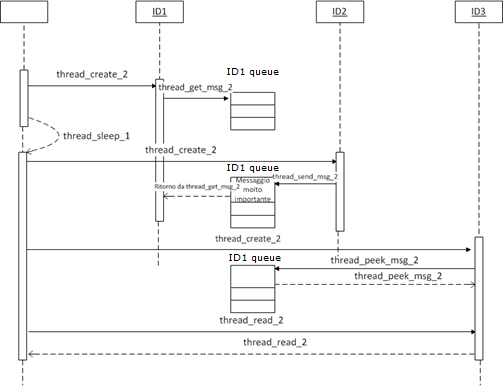
\includegraphics[width=12cm]{images/thread-example}
\caption{Execution flows in the third example.}
\label{fig:thread-example}
\end{figure}

\begin{verbatim}
start(X):- thread_create(ID1, thread1(ID1)),
           thread_sleep(200),
           thread_create(ID2, thread2(ID1)),
           thread_create(ID3, thread3(ID1,X)),
           thread_read(ID3, _),
           write('Father: done').

thread1(ID):- tell('threadLog.txt'),
              write('ID1: waiting for message'),
              thread_get_msg(ID, m(X)),
              write('ID1: message retrieved').

thread2(ID):- thread_send_msg( ID, m('critical message')),
              write('ID2: message sent').		

thread3(ID,X):- thread_peek_msg( ID, m(X)),
                write('ID3: trying to get message').
\end{verbatim}

More in detail, the father creates three threads identified by \texttt{ID1}, \texttt{ID2}, and \texttt{ID3}, which execute the goals \texttt{thread1/1}, \texttt{thread2/1}, and \texttt{thread3/2}, respectively: \texttt{ID1} is the message receiver/logger, \texttt{ID2} is the message sender, \texttt{ID3} is the task charged to monitor its brother's queue. To prevent races, the father waits for 200 ms after creating the first (message receiver) thread \texttt{ID1}, so that it is surely up and running when the message sender \texttt{ID2} and its brother \texttt{ID3} actually start.
Then, the father suspends its execution, waiting for \texttt{ID3} to terminate.

However, since \texttt{ID1} removes the message from its queue when reading (via \texttt{thread\_get\_msg/2}), \texttt{ID3} never finds anything when checking its brother's queue (via the non-blocking \texttt{thread\_peek\_msg/2} primitive): thus, its goal \texttt{thread3/2} always fails, causing the father's \texttt{thread\_read} to fail, too. As a result, the father's final write is never performed, either:

\begin{verbatim}
?- start(X).
no
\end{verbatim}
%
and the log file finally contains just

\begin{verbatim}
ID1: waiting for message
ID2: message sent
ID1: message retrieved
\end{verbatim}


%-------------------------------
\subsubsection{Synchronizing thread interactions}
%-------------------------------

In this producer/consumer example, the consumer's goal is to retrieve only the \textit{last} solution of the query \texttt{has\_child(bob,X)}, while the producer computes all the solutions to this query; the father coordinates the two tasks, by first creating the producer and the consumer, and then triggering the producer to generate all the possible solutions in sequence.

Without an explicit synchronisation mechanism, races would occur, causing the reader to read not \textit{the last} solution, but just ``one of'' the possible solutions, depending which thread is faster.

By suitably sequentialising the access to the producer's queue, the \texttt{mutex} semaphore guarantees that all solutions are produced \textit{before} the consumer can start reading, so that the last solution is actually read. (The execution flow diagram and the complete code are reported in Figure \ref{fig:thread-exampleMutex} on page \pageref{fig:thread-exampleMutex}.)

\begin{figure}
\centering
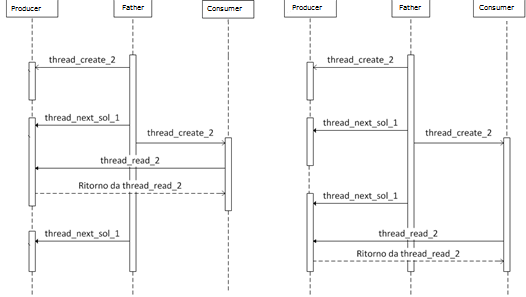
\includegraphics[width=13cm]{images/thread-exampleMutex}
\caption{Execution flows in the mutex example.}
%\label{fig:thread-exampleMutex}
%\end{figure}

\begin{Verbatim}[frame=single, samepage=true]
start:- thread_create(ID1, has_child(bob,X)),
        mutex_lock('mutex'),
        thread_create(ID2, read_child(ID1,X)),
        loop(1,5,1, ID1),
        mutex_unlock('mutex').

read_child(ID, X) :- mutex_lock('mutex'),
                     thread_read(ID, X),
                     mutex_unlock('mutex').

has_child(bob, alex).
has_child(bob, anna).
has_child(bob, mary).

loop(I, To, Inc, ThreadId) :- Inc >= 0, I > To, !.
loop(I, To, Inc, ThreadId) :- Inc < 0,  I < To, !.
loop(I, To, Inc, ThreadId) :-
  (thread_has_next(ThreadId) -> thread_next_sol(ThreadId),
                                Next is I+Inc,
                                loop(Next, To, Inc, ThreadId)
                              ; !).
\end{Verbatim}

\label{fig:thread-exampleMutex}
\end{figure}

The first child, \texttt{ID1}, is the solution finder \& producer: its task is to generate the solutions of the given goal \texttt{has\_child(bob,X)}. When started, it looks for the first solution: once found, it suspends waiting for possible future requests for alternative solutions. These will be actually asked shortly, since the father triggers \texttt{ID1} to find all the alternative solutions (via the \texttt{loop/4} predicate, which embeds a call to \texttt{thread\_next\_sol}) just after generating its second child, the solution reader thread \texttt{ID2}.
In fact, \texttt{ID2}'s task is to retrieve the computed solution from \texttt{ID1}'s private queue: but due to the \texttt{thread\_read} semantics, it actually reads \texttt{ID1}'s result only when \texttt{ID1} has terminated. This is why explicit synchronisation is needed: otherwise, the reader would read ``one of'' the solutions, non-deterministically, depending on which thread is faster (this can be easily checked by commenting out the \texttt{mutex\_lock}/\texttt{mutex\_unlock} statements).

With the explicit \texttt{mutex} semaphore, interactions are sequentialised: as long as the father holds the lock, the reader cannot retrieve any solution. Since the lock is released only after all the solutions have been explored, the reader will actually get only the last computed solution, \texttt{X / mary}.

%-------------------------------
\subsubsection{Flattening and manipulating lists}
%-------------------------------

Table \ref{tab:thread-exampleFlatList} on page \pageref{tab:thread-exampleFlatList} shows a sequential Prolog program that manipulates a list of (sub)lists. More precisely, it first flattens the list of lists into a single flat list, then sorts the obtained list and counts the occurrence of a given term in that list.

\begin{table}\small
\begin{Verbatim}[frame=single, samepage=true]
start(L, 0, T) :- !.
start([H|Tail], N, T) :-
    plain(H,L_plain),
    bubble(L_plain,L_ord),
    occurr_count(T,H,Count),
    C is N-1, start(Tail,C, T).

plain(L1,L2) :- plain(L1,[],L2).

plain([],ACC,ACC).
plain([H|REST],ACC,L2) :-
    H = [_|_],
    plain(H,ACC,ACC1),
    plain(REST,ACC1,L2).
plain([H|REST],ACC,L2) :-
    append(ACC,[H],ACC1),
    plain(REST,ACC1,L2).
plain(X,ACC,L2) :-
    append(ACC,[X],L2).

bubble(L1,L2) :- bubble(L1,0,L2).

bubble(L1,0,L2) :-
    sweep(L1,0,L2).
bubble(L1,0,L2) :-
    sweep(L1,1,LTMP),
    bubble(LTMP,0,L2).

sweep([X|[]],0,[X|[]]).
sweep([X,Y|REST1],CHANGED,[X|REST2]) :-
    X =< Y, sweep([Y|REST1],CHANGED,REST2).
sweep([X,Y|REST1],1,[Y|REST2]) :-
    X > Y, sweep([X|REST1],_,REST2).

occurr_count(T,L,N) :- occurr_count(T,L,0,N).

occurr_count(_,[],ACC,ACC).
occurr_count(T,[T|REST],ACC,N) :-
    ACC1 is ACC+1, occurr_count(T,REST,ACC1,N).
occurr_count(T,[_|REST],ACC,N) :- occurr_count(T,REST,ACC,N).
\end{Verbatim}
\caption{The sequential version of the list manipulation program.\\
         Query: \texttt{?- start([[[2,2],2,2,1],[4,[3],2],[9,8,9,2]], 3, 2).}}
\label{tab:thread-exampleFlatList}
\end{table}

To exploit concurrency, the program needs to be restructured, distributing the responsibilities among different threads.
As an example, we decided to delegate the list flattening and sorting to a child thread, maintaining the final occurrence counting on the main (father)'s thread: the result is shown in Table \ref{tab:thread-exampleFlatListConcurrent} on page \pageref{tab:thread-exampleFlatListConcurrent}, where the sequential and the concurrent versions are compared. The concurrent version showed a 16\% performance gain.

\begin{table}\small
\textit{Sequential version:}
\begin{Verbatim}[frame=single, samepage=true]
start(L, 0, T) :- !.
start([H|Tail], N, T) :-
    plain(H,L_plain),
    bubble(L_plain,L_ord),
    occurr_count(T,H,Count),
    C is N-1, start(Tail,C, T).
...
\end{Verbatim}

\textit{Concurrent version:}
\begin{Verbatim}[frame=single, samepage=true]
start(L, N, T) :-
    thread_create(ID, firstResp(L, N)),
    secondResp(L, N, T).

secondResp(L, 0, T):- !.
secondResp([H|Tail], N, T) :-
    occurr_count(T,H,Count),
    C is N-1, secondResp(Tail,C, T).

firstResp(L, 0) :- !.
firstResp([H|Tail], N) :-
    plain(H,L_plain),
    bubble(L_plain,L_ord),
    C is N-1, firstResp(Tail,C).
...
\end{Verbatim}
\caption{The sequential version (top) and the concurrent (bottom) version of the list manipulation program.\\
         Query: \texttt{?- start([[[2,2],2,2,1],[4,[3],2],[9,8,9,2]], 3, 2).}}
\label{tab:thread-exampleFlatListConcurrent}
\end{table}




%---------------------------------------------------------------------
\section{DCGLibrary}
\label{sec:dgc-library}
%---------------------------------------------------------------------

\noindent \emph{Library Dependencies}: BasicLibrary.

This library provides support for Definite Clause Grammars (DCGs) \cite{bra00}, an extension of context free grammars that have proven useful for describing natural and formal languages, and that may be conveniently expressed and executed in Prolog.
%
Note that this library is not loaded by default when a \tuprolog{} engine is created: it must be explicitly loaded by the user, or via a \texttt{load\_library} directive inside any theory using DCGs.

A DCG rule has the general form \verb|Head --> Body|: to distinguish terminal from nonterminal symbols, a phrase (that is, a sequence of terminal symbols) must be written as a Prolog list, with the empty sequence written as the empty list \verb|[]|.
%
The body can contain also executable blocks in parentheses, which are interpreted as normal Prolog rules.

Here is a simple example (see also Figure \ref{fig:dcg-example} on page \pageref{fig:dcg-example}):
%
\begin{verbatim}
    sentence --> noun_phrase, verb_phrase.
    verb_phrase --> verb, noun_phrase.
    noun_phrase --> [charles].
    noun_phrase --> [linda].
    verb --> [loves].
\end{verbatim}
%
To verify whether a phrase is correct according to the given grammar, the \texttt{phrase/2} or \texttt{phrase/3} predicates are used---the latter form providing an extra argument for the `remainder' of the input string not recognised as being part of the phrase.
%
Some examples follow:\\

\verb|?- phrase(sentence, [charles, loves, linda])|

\texttt{\textit{yes}}\\

\verb|?- phrase(sentence, [Who, loves, linda])|

\texttt{\textit{Who/charles}}

\texttt{\textit{Who/linda}}\\

\verb|?- phrase(sentence, [charles, loves, linda, but, hates, laura], R)|

\texttt{\textit{R/[but, hates, laura]}}\\

\begin{figure}
\centering
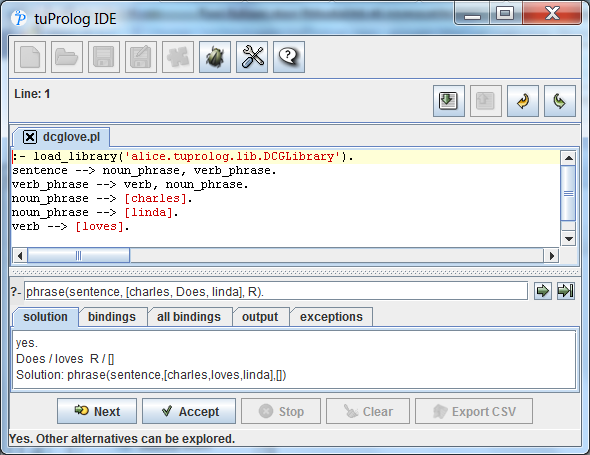
\includegraphics[width=7cm]{images/dcg-example}
\caption{The DCG Library example in the \tuprolog{} GUI (note the explicit library loading directive).}
\label{fig:dcg-example}
\end{figure}

%---------------------------------------------------------------------
\subsection{Predicates}
%---------------------------------------------------------------------

\noindent The classic built-in predicates provided for parsing DCG
sentences are:

\begin{itemize}
%
\item \bti{phrase/2}\\
    \noindent\bt{phrase(Category, List)} is true iff the list \bt{List} can be parsed as a phrase (i.e. sequence of terminals) of type \bt{Category}.
    \bt{Category} can be any term which would be accepted as a nonterminal of the grammar (or in general, it can be any grammar rule body), and must be instantiated to a non-variable term at the time of the call.
    This predicate is the usual way to commence execution of grammar rules.
    If \bt{List} is bound to a list of terminals by the time of the call, the goal corresponds to parsing \bt{List} as a phrase of type \bt{Category}; otherwise if \bt{List} is unbound, then the grammar is being used for generation.

    \template{phrase(+term, ?list)}

    \exception{error(instantiation\_error, instantiation\_error(\\
    Goal, ArgNo))} if \texttt{Category} is a variable. \texttt{Goal} is the goal where the problem occurred, \texttt{ArgNo} indicates the argument that caused the problem (obviously, \texttt{1}).

\item \bti{phrase/3}\\
    \noindent\bt{phrase(Category, List, Rest)} is true iff the segment between the start of list \bt{List} and the start of list \bt{Rest} can be parsed as a phrase (i.e. sequence of terminals) of type \bt{Category}.
    In other words, if the search for phrase Phrase is started at the beginning of list \bt{List}, then \bt{Rest} is what remains unparsed after \bt{Category} has been found.
    Again, \bt{Category} can be any term which would be accepted as a nonterminal of the grammar (or in general, any grammar rule body), and must be instantiated to a non variable term at the time of the call.

    \template{phrase(+term, ?list, ?rest)}

    \exception{error(instantiation\_error, instantiation\_error(\\
    Goal, ArgNo))} if \texttt{Category} is a variable. \texttt{Goal} is the goal where the problem occurred, \texttt{ArgNo} indicates the argument that caused the problem (obviously, \texttt{1}).

\end{itemize}

%---------------------------------------------------------------------
\subsection{Operators}
%---------------------------------------------------------------------

The full list of DCGLibrary operators, with their priority and associativity, is reported in Table \ref{tab:dcglibrary-operators}.

\begin{table}[h]
    \begin{center}{\small\tt
    \begin{tabular}{p{2cm}|p{3cm}|p{3cm}}\hline\hline
    Operator & Associativity & Priority \\ \hline
    --> & xfx & 1200\\
    \hline\hline
    \end{tabular}
    }\end{center}
    \caption{DCGLibrary operators.}\label{tab:dcglibrary-operators}
\end{table}


%---------------------------------------------------------------------
\section{ISOIOLibrary}
\label{sec:isoio-library}
%---------------------------------------------------------------------

The ISO specification requires a lot of I/O predicates---many more than \tuprolog{} IOLibrary supports.
%
Table \ref{fig:isoiolibrary-table} summarises the differences between \tuprolog{} IOLibrary and the ISO specifications.
%
\begin{figure}
  \centering
  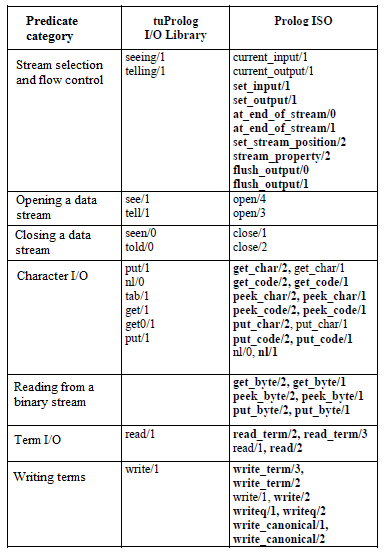
\includegraphics[width=10cm]{images/isoiolibrary-table}
  \caption{Comparison between the I/O predicates provided by IOLibrary and the ISO standard specification. Bold style indicates missing predicates, plain style indicates existing functionalities to be refactored, improved, or be provided with a different signature to be ISO-compliant.}\label{fig:isoiolibrary-table}
\end{figure}
%
The main reason for such a large number of differences is that the ISO Prolog standard defines very general concepts for I/O handling, aimed at supporting a wide variety of I/O modes and devices. More precisely:
\begin{itemize}
  \item \textbf{Sources} represent the resources from which data are read;
  \item \textbf{Sinks} represent the resources to which data are written.
\end{itemize}
%
Sources and sinks can be file, standard input/output stream, or any other resource supported by the underlying system: the only assumption is that each resource is associated to a sequence of bytes or characters.

\textit{Stream terms} provide a logical view of sources and sinks, and are used to identify a stream in I/O predicates. A stream term is a term respecting the following constraints:
\begin{itemize}
  \item it is a ground term;
  \item it is not an atom (this requirement means to distinguish stream terms from stream aliases--see below for details);
  \item it is not used to identify other streams at the same time.
\end{itemize}
%
The ISO standard does not specify whether the stream terms must result from an explicit source/sink opening by the \texttt{open/4} predicate, nor whether different sources/sinks must be represented by different stream terms at subsequent times: these issues are left to the specific implementation.

Moreover, each stream can be associated to a \textit{stream alias}---an atom used to refer to the stream. The association between a stream and its alias is created when the stream is opened, and automatically canceled when the stream is closed.
The same stream can be associated to multiple aliases simultaneously.
%
Two pre-defined streams exist that are always automatically open: the standard input (alias \texttt{user\_input}) and the standard output
(alias \texttt{user\_output}). Such streams must never be closed.

The ISO standard also introduces the concepts of \textit{current input stream} and \textit{current output stream}: initially, they default to the standard input and standard output above, but can be reassigned at any time via the \texttt{set\_input/1} e and \texttt{set\_output/1} predicates.
However, when such an input/output stream is closed, the current input/output stream must be re-set to its default value (i.e., the standard input/output, respectively).

One further concept is the \textit{stream position}, which defines the point where the next input/output will take place; syntactically, it is an implementation-dependent ground term.
The stream position is always supported, even by predicates whose operations do not change the position itself; to change the current position, the \texttt{set\_stream\_position/2} predicate is used.
When an output stream is repositioned, any output possibly present in the sink is overwritten; when an input stream is repositioned, instead, the content already available into the stream remains unaltered.

A stream that can be repositioned (that is, whose \texttt{reposition} property is true) must support also the \textit{end position} concept: the position of an input stream that has been completely read is represented by the \texttt{end-of-stream} atom, while any attempt to read beyond the end of stream causes the stream position to become \texttt{past-end-of-stream}.

On the other hand, output streams can be \textit{flushed} when necessary via the \texttt{flush\_output/1} predicate; a stream is automatically flushed before closing.


%---------------------------------------------------------------------
\subsection{Predicates}
%---------------------------------------------------------------------

\noindent ISOIOLibrary defines the following predicates:

\begin{itemize}

\item \bti{current\_input/1}\\
    \noindent\bt{current\_input} unifies the current input stream with the given argument.

    \template{current\_input(@Stream\_or\_alias)}

\item \bti{current\_output/1}\\
    \noindent\bt{current\_output} unifies the current output stream with the given argument.

    \template{current\_output(@Stream\_or\_alias)}


\item \bti{set\_input/1}\\
    \noindent\bt{set\_input} associates the current input to the provided argument, which can be either a stream\_term or an alias.

    \template{set\_input(@Stream\_or\_alias)}

    \exception{error(instantiation\_error, instantiation\_error)} if \textit{\texttt{Stream\_or\_alias}} is a variable.

    \exception{error(domain\_error, domain\_error(\texttt{stream\_or\_alias},\\
    \texttt{\textit{Stream\_or\_alias}}))} if \textit{\texttt{Stream\_or\_alias}} is neither a stream term nor a valid stream alias.

    \exception{error(existence\_error, existence\_error(\texttt{stream},\\
    \texttt{\textit{Stream\_or\_alias}}))} if \textit{\texttt{Stream\_or\_alias}} is not associated to an open stream.

    \exception{error(permission\_error, permission\_error(\texttt{input},\\
    \texttt{stream}, \texttt{\textit{Stream\_or\_alias}}))} if \textit{\texttt{Stream\_or\_alias}} is associated to an output stream.


\item \bti{set\_output/1}\\
    \noindent\bt{set\_output} associates the current output to the provided argument, which can be either a stream\_term or an alias.

    \template{set\_output(@Stream\_or\_alias)}

    \exception{error(instantiation\_error, instantiation\_error)} if \textit{\texttt{Stream\_or\_alias}} is a variable.

    \exception{error(domain\_error, domain\_error(\texttt{stream\_or\_alias},\\
    \texttt{\textit{Stream\_or\_alias}}))} if \textit{\texttt{Stream\_or\_alias}} is neither a stream term nor a valid stream alias.

    \exception{error(existence\_error, existence\_error(\texttt{stream},\\
    \texttt{\textit{Stream\_or\_alias}}))} if \textit{\texttt{Stream\_or\_alias}} is not associated to an open stream.

    \exception{error(permission\_error, permission\_error(\texttt{output},\\
    \texttt{stream}, \texttt{\textit{Stream\_or\_alias}}))} if \textit{\texttt{Stream\_or\_alias}} is associated to an input stream.

\item \bti{flush\_output/0} - \bti{flush\_output/1}\\
    \noindent\bt{flush\_output} flushes the output onto the stream associated to the provided argument, which can be either a stream\_term or an alias; if no argument is provided, the default output stream is flushed.

    \template{flush\_output(@Stream\_or\_alias)}\\
    \template{flush\_output}

    \exception{error(instantiation\_error, instantiation\_error)} if \textit{\texttt{Stream\_or\_alias}} is a variable.

    \exception{error(domain\_error, domain\_error(\texttt{stream\_or\_alias},\\
    \texttt{\textit{Stream\_or\_alias}}))} if \textit{\texttt{Stream\_or\_alias}} is not a valid stream term or alias.

    \exception{error(existence\_error, existence\_error(\texttt{stream},\\
    \texttt{\textit{Stream\_or\_alias}}))} if \textit{\texttt{Stream\_or\_alias}} is not associated to an open stream.

    \exception{error(permission\_error, permission\_error(\texttt{output},\\
    \texttt{stream}, \texttt{\textit{Stream\_or\_alias}}))} if \textit{\texttt{Stream\_or\_alias}} is associated to an input stream.


\item \bti{stream\_property/2}\\
    \noindent\bt{stream\_property} verifies whether the given stream has the given property, unifying \textit{\texttt{Property}} with the corresponding value.

    \template{stream\_property(?Stream, ?Property)}

    \exception{error(instantiation\_error, instantiation\_error)} if \textit{\texttt{Stream}} is a variable.

    \exception{error(domain\_error, domain\_error(\texttt{stream},\\
    \texttt{\textit{Stream}}))} if \textit{\texttt{Stream}} is not a stream term.

    \exception{error(domain\_error, domain\_error(\texttt{stream\_property},\\
    \texttt{\textit{Property}}))} if \textit{\texttt{Property}} is neither a variable nor a stream property.

    \exception{error(existence\_error, existence\_error(\texttt{stream},\\
    \texttt{\textit{Stream}}))} if \textit{\texttt{Stream}} is not associated to an open stream.


\item \bti{at\_end\_of\_stream/0} - \bti{at\_end\_of\_stream/1}\\
    \noindent\bt{at\_end\_of\_stream} succeeds if the \texttt{end\_of\_stream} property has either the \texttt{end\_of\_stream} or the \texttt{past\_end\_of\_stream} value. The zero-argument version checks the current input stream.

    \template{at\_end\_of\_stream(@Stream\_or\_alias)}\\
    \template{at\_end\_of\_stream}

    \exception{error(instantiation\_error, instantiation\_error)} if \textit{\texttt{Stream\_or\_alias}} is a variable.

    \exception{error(domain\_error, domain\_error(\texttt{stream},\\
    \texttt{\textit{Stream\_or\_alias}}))} if \textit{\texttt{Stream\_or\_alias}} is not a valid stream term or alias.

    \exception{error(existence\_error, existence\_error(\texttt{stream},\\
    \texttt{\textit{Stream\_or\_alias}}))} if \textit{\texttt{Stream\_or\_alias}} is not associated to an open stream.


\item \bti{set\_stream\_position/2}\\
    \noindent\bt{set\_stream\_position} is true if the stream position can be successfully set to the new \texttt{\textit{Position}} argument.

    \template{set\_stream\_position(@Stream\_or\_alias, @Position)}

    \exception{error(instantiation\_error, instantiation\_error)} if either \textit{\texttt{Stream\_or\_alias}} or \textit{\texttt{Position}} is a variable.

    \exception{error(domain\_error, domain\_error(\texttt{stream},\\
    \texttt{\textit{Stream\_or\_alias}}))} if \textit{\texttt{Stream\_or\_alias}} is not a valid stream term or alias.

    \exception{error(existence\_error, existence\_error(\texttt{stream},\\
    \texttt{\textit{Stream\_or\_alias}}))} if \textit{\texttt{Position}} is neither a valid stream position, nor a variable.

    \exception{error(permission\_error, permission\_error(\texttt{reposition},\\
    \texttt{stream}, \texttt{\textit{Stream\_or\_alias}}))} if the \texttt{reposition} property of this stream is false.


\item \bti{open/3} - \bti{open/4}\\
    \noindent\bt{open} succeeds if the stream can be opened according to the \texttt{mode} and \texttt{options} desired.

    \template{open(@Source\_Sink, @Mode, -Stream)}\\
    \template{open(@Source\_Sink, @Mode, -Stream, @Options)}

    \exception{error(instantiation\_error, instantiation\_error)} if either \textit{\texttt{Source\_sink}} or \textit{\texttt{Mode}} is a variable, or if \texttt{\textit{Options}} is a partial list or such a list contains a variable.

    \exception{error(type\_error, type\_error(atom, Mode))} if \textit{\texttt{Mode}} is a neither an atom nor a variable.

    \exception{error(type\_error, type\_error(list, Options))} if\\ \texttt{\textit{Options}} is neither a list nor a partial list.

    \exception{error(type\_error, type\_error(variable, Stream))} if \texttt{\textit{Stream}} is not a variable.

    \exception{error(domain\_error, domain\_error(\texttt{stream\_sink},\\
    \texttt{\textit{Source\_sink}}))} if \textit{\texttt{Source\_sink}} is not a valid stream source or sink.

    \exception{error(domain\_error, domain\_error(\texttt{io\_mode},\\
    \texttt{\textit{Mode}}))} if \textit{\texttt{Mode}} is an atom other than the prescribed \texttt{input} or \texttt{output}.

    \exception{error(domain\_error, domain\_error(\texttt{stream\_option},\\
    \texttt{\textit{Element}}))} if an \textit{\texttt{Element}} of the options list is neither a variable nor a valid stream option.

    \exception{error(existence\_error, existence\_error(\texttt{stream},\\
    \texttt{\textit{Source\_sink}}))} if the source /sink stream \textit{\texttt{Source\_sink}} does not exist.

    \exception{error(permission\_error, permission\_error(\texttt{open},\\
    \texttt{source\_sink}, \texttt{\textit{Source\_sink}}))} if the specified source/sink stream cannot be opened.

    \exception{error(permission\_error, permission\_error(\texttt{open},\\
    \texttt{source\_sink}, \texttt{alias(\textit{A})}))} if \texttt{alias(\textit{A})} is in the options list, and \texttt{\textit{A}} is already bound to another open stream.

    \exception{error(permission\_error, permission\_error(\texttt{open},\\
    \texttt{source\_sink}, \texttt{reposition(true)}))} if \texttt{reposition(true)} is in the options list, but the stream cannot be repositioned.


\item \bti{close/1} - \bti{close/2}\\
    \noindent\bt{close} closes the given stream, eliminating any associated alias(es).
    If the \texttt{force(true)} option is specified, the stream is immediately closed, ignoring any data not yet transferred (in the case of output streams); in any other case, the stream is flushed before closing. If the stream to be closed is the current stream, the latter will be associated to the standard input or output, as appropriate.

    \template{close(@Stream\_or\_alias)}\\
    \template{close(@Stream\_or\_alias, @Options)}

    \exception{error(instantiation\_error, instantiation\_error)} if either \textit{\texttt{Stream\_or\_alias}} is a variable, or \texttt{\textit{Options}} is a partial list or such a list contains a variable.

    \exception{error(type\_error, type\_error(list, Options))} if\\ \texttt{\textit{Options}} is neither a list nor a partial list.

    \exception{error(domain\_error, domain\_error(\texttt{stream\_or\_alias},\\
    \texttt{\textit{Stream\_or\_alias}}))} if \textit{\texttt{Stream\_or\_alias}} is not a valid stream term or alias.

    \exception{error(domain\_error, domain\_error(\texttt{close\_option},\\
    \texttt{\textit{Element}}))} if an \textit{\texttt{Element}} of the options list is neither a variable nor a valid close option.

    \exception{error(existence\_error, existence\_error(\texttt{stream},\\
    \texttt{\textit{Stream\_or\_alias}}))} if the stream \textit{\texttt{Stream\_or\_alias}} is not associated to an open stream.

    \exception{error(permission\_error, permission\_error(\texttt{open},\\
    \texttt{source\_sink}, \texttt{\textit{Source\_sink}}))} if the specified source/sink stream cannot be opened.

    \exception{error(permission\_error, permission\_error(\texttt{open},\\
    \texttt{source\_sink}, \texttt{alias(\textit{A})}))} if \texttt{alias(\textit{A})} is in the options list, and \texttt{\textit{A}} is already bound to another open stream.

    \exception{error(permission\_error, permission\_error(\texttt{open},\\
    \texttt{source\_sink}, \texttt{reposition(true)}))} if \texttt{reposition(true)} is in the options list, but the stream cannot be repositioned.


\item \bti{get\_char/2} - \bti{get\_char/1} - \bti{get\_code/2} - \bti{get\_code/1}\\
    \noindent\bt{get\_char} and \bt{get\_code} read the next char from the given stream, and unify it with the second argument---a character or an integer representing the character code, respectively; the single-argument version of these predicates read from the current input stream. Special cases are treated as follows:
    \begin{itemize}
      \item if the stream position is \texttt{past\_end\_of\_stream}, the action to be performed depends on the stream options specified when the stream was opened---namely, \texttt{eof\_action(\textit{Action})}(see above);
      \item if the stream position is \texttt{end\_of\_stream}, the EOF character is returned, and the stream position becomes \texttt{past\_end\_of\_stream}.
    \end{itemize}

    \template{get\_char(@Stream\_or\_alias, ?Character)}\\
    \template{get\_char(?Character)}\\
    \template{get\_code(@Stream\_or\_alias, ?Character\_code)}\\
    \template{get\_code(?Character\_code)}

    \exception{error(instantiation\_error, instantiation\_error)} if either \textit{\texttt{Stream\_or\_alias}} is a variable.

    \exception{error(type\_error, type\_error(in\_character, \textit{Character}))} if \texttt{\textit{Character}} is neither a variable nor a character.

    \exception{error(type\_error, type\_error(integer, \textit{Character\_code}))} if \texttt{\textit{Character\_code}} is neither a variable nor an integer.

    \exception{error(domain\_error, domain\_error(\texttt{stream\_or\_alias},\\
    \texttt{\textit{Stream\_or\_alias}}))} if \textit{\texttt{Stream\_or\_alias}} is not a valid stream term or alias.

    \exception{error(existence\_error, existence\_error(\texttt{stream},\\
    \texttt{\textit{Stream\_or\_alias}}))} if the stream \textit{\texttt{Stream\_or\_alias}} is not associated to an open stream.

    \exception{error(permission\_error, permission\_error(\texttt{input},\\
    \texttt{stream}, \texttt{\textit{Stream\_or\_alias}}))} if the stream in not an input stream.

    \exception{error(permission\_error, permission\_error(\texttt{input},\\
    \texttt{binary\_stream}, \texttt{\textit{Stream\_or\_alias}}))} if the stream in not a text stream.

    \exception{error(permission\_error, permission\_error(\texttt{input},\\
    \texttt{past\_end\_of\_stream}, \texttt{\textit{Stream\_or\_alias}}))} if the stream status is\\
    \texttt{end\_of\_stream(past)} and the option \texttt{eof\_action(true)} is active.

    \exception{error(representation\_error,  representation\_error(\texttt{\textit{\\
    Character}}))} if the entity read from the stream is not a character.

    \exception{error(representation\_error,  representation\_error(\texttt{\textit{\\
    Character\_code}}))} if the entity read from the input stream is an integer, but does not represent a character.


\item \bti{peek\_char/2} - \bti{peek\_char/1} - \bti{peek\_code/2} - \bti{peek\_code/1}\\
    \noindent\bt{peek\_char} and \bt{peek\_code} work identically to the \texttt{get\_char} and \texttt{get\_code} above, but leave the stream position unaltered after reading, so that a subsequent read operation returns the same character.

    \template{peek\_char(@Stream\_or\_alias, ?Character)}\\
    \template{peek\_char(?Character)}\\
    \template{peek\_code(@Stream\_or\_alias, ?Character\_code)}\\
    \template{peek\_code(?Character\_code)}

    \exception{}: the same as above.


\item \bti{put\_char/2} - \bti{put\_char/1} - \bti{put\_code/2} - \bti{put\_code/1}\\
    \noindent\bt{put\_char} and \bt{put\_code} are the writing counterparts of the \texttt{get\_char} and \texttt{get\_code} above; syntax and exceptions raised are basically identical, but the \texttt{Character} or \texttt{Character\_code} must be ground in this case---otherwise, an \texttt{instantiation\_error} occurs.

    \template{put\_char(@Stream\_or\_alias, +Character)}\\
    \template{put\_char(+Character)}\\
    \template{put\_code(@Stream\_or\_alias, +Character\_code)}\\
    \template{put\_code(+Character\_code)}

    \exception{}: the same as above, plus an \texttt{error(instantiation\_error, instantiation\_error)} if \texttt{Character} or \texttt{Character\_code} is a variable.

\item \bti{nl/0} - \bti{nl/1}\\
    \noindent\bt{nl} inserts a newline in the given stream.

    \template{nl(@Stream\_or\_alias)}\\
    \template{nl}

    \exception{error(instantiation\_error, instantiation\_error)} if either \textit{\texttt{Stream\_or\_alias}} is a variable.


\item \bti{read\_term/2} - \bti{read\_term/3} - \bti{read/1} - \bti{read/2}\\
    \noindent\bt{read\_term} succeeds if a term can be read from the given stream that can be unified with the \texttt{\textit{Term}} argument: \texttt{\textit{Options}} are considered only if the above unification succeeds. The \texttt{read} predicate works analogously, but no options can be specified. As usual, the no-stream versions (\bti{read\_term/2} and \bti{read/1}) operate on the current input stream.

    \template{read\_term(@Stream\_or\_alias, ?Term, +Options)}\\
    \template{read\_term(?Term, +Options)}\\
    \template{read(@Stream\_or\_alias, ?Term)}\\
    \template{read(?Term)}

    \exception{error(instantiation\_error, instantiation\_error)} if either \textit{\texttt{Stream\_or\_alias}} is a variable.

    \exception{error(instantiation\_error, instantiation\_error)} if \texttt{\textit{Options}} is either a partial list, or an element in the list is a variable.

    \exception{error(type\_error, type\_error(list, \textit{Options}))} if\\ \texttt{\textit{Options}} is neither a list nor a partial list.

    \exception{error(domain\_error, domain\_error(\texttt{stream\_or\_alias},\\
    \texttt{\textit{Stream\_or\_alias}}))} if \textit{\texttt{Stream\_or\_alias}} is not a valid stream term or alias.

    \exception{error(existence\_error, existence\_error(\texttt{stream},\\
    \texttt{\textit{Stream\_or\_alias}}))} if the stream \textit{\texttt{Stream\_or\_alias}} is not associated to an open stream.

    \exception{error(domain\_error, domain\_error(\texttt{read\_option},\\
    \texttt{\textit{Element}}))} if an element in the option list is neither a variable nor a valid read option.

    \exception{error(existence\_error, existence\_error(\texttt{stream},\\
    \texttt{\textit{Stream\_or\_alias}}))} if \textit{\texttt{Stream\_or\_alias}} is not associated to an open stream.

    \exception{error(permission\_error, permission\_error(\texttt{input},\\
    \texttt{stream}, \texttt{\textit{Stream\_or\_alias}}))} if the stream in not an input stream.

    \exception{error(permission\_error, permission\_error(\texttt{input},\\
    \texttt{binary\_stream}, \texttt{\textit{Stream\_or\_alias}}))} if the stream in not a text stream.

    \exception{error(permission\_error, permission\_error(\texttt{input},\\
    \texttt{past\_end\_of\_stream}, \texttt{\textit{Stream\_or\_alias}}))} if the stream status is\\
    \texttt{end\_of\_stream(past)} and the option \texttt{eof\_action(true)} is active.

    \exception{error(representation\_error,  representation\_error(\texttt{\textit{\\
    Flag}}))} if the entity read from the stream does not comply with the rules expressed by \texttt{\textit{Flag}}, which can be \texttt{max\_arity}, \texttt{max\_integer}, \texttt{min\_integer}.

    \exception{error(representation\_error,  representation\_error(\texttt{
    imp\_dep\_atom}))} if one or more characters in the input stream cannot form a valid token, or the character sequence cannot be transformed into a valid atom according to the current operator notation.

\item \bti{write\_term/2} - \bti{write\_term/3} - \bti{write/1} - \bti{write/2} - \bti{writeq/1} - \bti{writeq/2} - \bti{write\_canonical/1} - \bti{write\_canonical/2}\\
    These predicates are the writing counterparts of the \texttt{read\_term} and \texttt{read} predicates above: the given term is written on the given stream according to the specified write options, or following the default values\footnote{Namely: \texttt{quoted(false)}, \texttt{ignore\_ops(false)}, \texttt{numbervars(true)} for \texttt{write}, \texttt{quoted(true)}, \texttt{ignore\_ops(false)}, \texttt{numbervars(true)} for \texttt{writeq}, \texttt{quoted(true)}, \texttt{ignore\_ops(true)}, \texttt{numbervars(true)} for \texttt{write\_canonical}.} in the \texttt{write}, \texttt{writeq} and \texttt{write\_canonical} cases. Basically, the same considerations and exceptions above still apply.

    \template{write\_term(@Stream\_or\_alias, @Term, +Options)}\\
    \template{write\_term(@Term, +Options)}\\
    \template{write(@Stream\_or\_alias, @Term)}\\
    \template{write(@Term)}
    \template{writeq(@Stream\_or\_alias, @Term)}\\
    \template{writeq(@Term)}

    \exception{}: the same as above

%---------------------------------------------------------------------
%\subsubsection{Writing terms}
%---------------------------------------------------------------------

    When a term is written via \texttt{write\_term/3}, the following rules apply:

    \begin{itemize}
      \item if the term is a variable, a character is produced of the form \texttt{\_\textit{string}} where the string following the underscore are implementation-dependent. A variable occurring multiple times in the term is obviously converted into the same \texttt{\_\textit{string}} for each occurrence.
      \item if the term is an integer number, the corresponding string is produced; negative values starts with \texttt{-}.
      \item if the term is a real number, the corresponding string is produced; negative values starts with \texttt{-}. If the write option \texttt{quoted} is true, the produced string ensures that a subsequent \texttt{read\_term} can read it back correctly.
      \item if the term is an atom that could not be read back unless quoted, and the write option \texttt{quoted} is true, the produced string is quoted; otherwise it is not.
      \item if the term contains a main functor that \textit{is not} an operator, or the write option \texttt{ignore\_ops} is true, the term is written in the \textit{canonical form} (Table \ref{tab:isoiolibrary-write-terms}); otherwise it is not.
      \item if, instead, the term contains a main that \textit{is} an operator and the write option \texttt{ignore\_ops} is true, the term is written in the operator notation ((Table \ref{tab:isoiolibrary-write-terms}).
    \end{itemize}

    \begin{table}
      \footnotesize\centering
      \begin{tabular}{|p{6cm}|p{6cm}|}
        \hline
        \textit{Canonical form} & \textit{Operator notation}\\
        \hline
        For every term other than lists: & - The operator itself is returned either before
        (for prefix operators), or between (for infix operators) or after (for postfix operators) its arguments;\\
        - the main functor's atom; &  - a space is always inserted between the operator and its arguments;\\
        - the open parenthesis \texttt{'('}; & - for each argument, the same rules above are applied recursively; \\
        - each term argument, built applying the same rules recursively, in a comma-separated list; & - if one of the argument is also an operator, it is enclosed between parentheses. \\
        - the closed parenthesis \texttt{')'}; & \\
        \textbf{Example:} \texttt{2+3} becomes \texttt{+(2,3)} & \\
        \hline
        For lists (e.g. terms of the form \texttt{�.�(Head, Tail)}), the list notation is used if the write option \texttt{ignore\_ops} is false: & \\
        - an open square bracket \texttt{'['}; &  \\
        - the head argument, built applying the same rules recursively; & \\
        - the tail argument, built as follows; & \\
        \mbox{~~}- if the tail has the form \texttt{�.�(Head, Tail)}), a comma is produced and the above rule is triggered recursively; & \\
        \mbox{~~}- otherwise, if the tail is empty (e.g. \texttt{[]}), a close bracket is produced \texttt{']'} & \\
        \mbox{~~}- otherwise, a pipe symbol is produced \texttt{'|'} and these rules are re-applied recursively; at the end, a close bracket is produced \texttt{']'} & \\
        \hline
      \end{tabular}
      \caption{Term writing rules: canonical form and operator notation.}
      \label{tab:isoiolibrary-write-terms}
\end{table}


\item \bti{get\_byte/2} - \bti{get\_byte/1} - \bti{peek\_byte/2} - \bti{peek\_byte/1} - \bti{put\_byte/2} - \bti{put\_byte/1}\\
    \noindent\bt{get\_byte}, \bt{peek\_byte} and \bt{put\_byte} are the binary counterparts of the \texttt{get\_char}, \texttt{peek\_char} and \texttt{put\_char} above; syntax and exceptions raised are basically identical, with obvious changes (i.e., the wrong type of stream here is \texttt{text} instead of \texttt{binary}).

    \template{get\_byte(@Stream\_or\_alias, ?Byte)}\\
    \template{get\_byte(?Byte)}\\
    \template{peek\_byte(@Stream\_or\_alias, ?Byte)}\\
    \template{peek\_byte(?Byte)}\\
    \template{put\_byte(@Stream\_or\_alias, +Byte)}\\
    \template{put\_byte(+Byte)}

    \exception{}: see description above.

\end{itemize}





%---------------------------------------------------------------------
\subsection{Options}
%---------------------------------------------------------------------

The ISO standard defines options for stream creation, stream closure, and stream properties.

\noindent When a stream is opened via \texttt{open/4}:

\begin{itemize}
 \item \texttt{type(\textit{Type})} specifies the stream type---either a binary stream or a text stream (default);
 \item \texttt{reposition(\textit{Bool})} specifies whether the stream can be repositioned or not (see above);
 \item \texttt{alias(\textit{Alias})} defines \texttt{\textit{Alias}} as a stream alias for this stream;
 \item \texttt{eof\_action(\textit{Action})} specifies the value to be returned by a read predicate encountering the end-of-stream; possible values are \texttt{error}, to indicate that no further read is possible, or \texttt{eof\_code} \textit{(default)}, to indicate that the special \texttt{eof} value must be returned, or \texttt{reset}, meaning that the read position must be reset to the start of the stream. This is particulary useful on the console input.
\end{itemize}

\noindent Conversely, when a stream is closed via \texttt{close/1}-\texttt{/2}:

\begin{itemize}
 \item \texttt{force(\textit{Bool})} specifies whether the stream must be forcedly closed upon error: the default is \textit{false}. If the value is set to \textit{true}, the stream might remain in an inconsistent state, or data may be lost, when the forced closing occurs.
\end{itemize}

\noindent Stream properties are expressed via the \texttt{stream\_property(\textit{Stream}, \textit{Property})} predicate, where \texttt{\textit{Property}} is one of the following:

\begin{itemize}
 \item \texttt{file\_name(\textit{File})} if the stream is connected to a file, returns a unique identifier of the file;

  \item \texttt{mode(\textit{Mode})} is to be specified when the stream is opened: \texttt{\textit{Mode}} can be \texttt{read}, \texttt{write} or \texttt{append};

  \item \texttt{input} if the stream is connected to a source;

  \item \texttt{output} if the stream is connected to a sink;

  \item \texttt{alias(\textit{Alias})} returns the stream alias, if the stream has one;

  \item \texttt{position(\textit{Pos})} returns the current stream position, if the stream can be repositioned;

  \item \texttt{end\_of\_stream(\textit{End})} returns either \texttt{not}, if the stream is not at the end, or \texttt{at}, if the stream is precisely at the end, or \texttt{past} if the stream is past the end of the stream;

  \item \texttt{eof\_action(\textit{Action})} returns the \texttt{\textit{Action}} specified when the stream was opened, if there was one, or an implementation-dependent action associated to the stream, otherwise;

  \item \texttt{reposition(\textit{Bool})} returns whether the stream can be repositioned (\texttt{true} or \texttt{false});

  \item \texttt{type(\textit{Type})} returns whether the stream is a \texttt{binary} stream or a \texttt{text} stream.
\end{itemize}

\noindent The standard input and output streams are configured as in Table \ref{tab:isoiolibrary-user-streams}.

\begin{table}
  \centering
  \begin{tabular}{|p{5cm}|p{5cm}|}
    \hline
    \textbf{\texttt{user\_input}} & \textbf{\texttt{user\_output}}\\
    \hline
    \texttt{mode(read)} & \texttt{mode(append)} \\
    \texttt{input} & \texttt{output} \\
    \texttt{alias(user\_input)} & \texttt{alias(user\_output)}\\
    \texttt{eof\_action(reset)} & \texttt{eof\_action(reset)}\\
    \texttt{reposition(false)} & \texttt{reposition(false)}\\
    \texttt{type(text)} & \texttt{type(text)}\\
    \hline
  \end{tabular}
  \caption{The default configuration of the standard I/O streams.}
  \label{tab:isoiolibrary-user-streams}
\end{table}


\noindent Read properties can be specified in read predicates like \texttt{read\_term}, and can have the following forms:

\begin{itemize}
 \item \texttt{variables(\textit{Vars})}: when a term is read, \texttt{\textit{Vars}} is the list of variables found in the term; anonymous variables are included;

 \item \texttt{variable\_names(\textit{VNList})}: when a term is read, \texttt{\textit{VNList}} is unified with a list of \texttt{A=V} pairs, where \texttt{A} is an atom denoting a variable name in term read, and \texttt{V} is the corresponding variable in the term template; anonymous variables are not included in the list;

 \item \texttt{singletons(\textit{VNList})}: when a term is read, \texttt{\textit{VNList}} is unified with a list of \texttt{A=V} pairs, where \texttt{A} is an atom denoting a variable name in term read, and \texttt{V} is the corresponding variable in the term template; anonymous variables are not included in the list.
\end{itemize}

\noindent For instance, if a query like:

\texttt{?:- read\_term(st, T, [variables(VL),\\
\mbox{~~~~~~~~~~~~~~~~~~~~~~~~~}variable\_names(VN), singletons(VS)].}

\noindent reads a term such as \texttt{foo(A+Roger, A+\_)}, the result is:

\noindent
\texttt{T  / foo(Xl+X2, X1+X3)}\\
\texttt{VL / [Xl, X2, X3]}\\
\texttt{VN / ['A' = Xl, 'Roger' = X2]}\\
\texttt{VS / ['Roger' = X2]}

\noindent Basically, the term read is scanned for variables, which are named according to some implementation-dependent template (e.g. \texttt{X1}, \texttt{X2}, \texttt{X3}); these names are used in the lists above, either to list all the variables (including the anonymous ones---see \texttt{X3} in \texttt{VL}), or to list the correspondence between the actual variable names and such placeholders (\texttt{VN} and \texttt{VS}, the latter including singleton variables only).

Analogously, write properties can be specified in write predicates like \texttt{write\_term}, and can have the following forms:

\begin{itemize}
 \item \texttt{quoted(\textit{Bool})}: specifies whether each atom of functor is quoted (usually because it comes from a previous \texttt{read\_term});

 \item \texttt{ignore\_ops(\textit{Bool})}: if true, each compound term is returned in a function notation. Any other option is ignored.

 \item \texttt{numbervars(\textit{Bool})}: if true, the terms of the form \texttt{'\$VAR'(N)} are replaced by a system-generated variable name that uses the \textit{N}th capital letter\footnote{\texttt{A} is considered the 0th letter.} followed by a the \texttt{N}/26 integer.
     For instance, \texttt{'\$VAR'(51)} produces \texttt{Z1}, since the 51th letter of the alphabet (mod 26) is \texttt{Z}, and 51/26=1.
\end{itemize}


%---------------------------------------------------------------------
\section{SocketLibrary}
\label{sec:socket-library}
%---------------------------------------------------------------------

\noindent \emph{Library Dependencies}: BasicLibrary.

This library provides support for TCP and UDP sockets. To this end, the library provides functionalities for
\begin{itemize}
  \item handling server sockets---namely, creating and closing a server socket, and accepting incoming connections;
  \item handling client sockets---namely, opening a socket establishing a connection to a given address;
  \item handling client/server communication, both in synchronous and asynchronous mode.
\end{itemize}

As an example, let us first consider the following TCP server-side code:\\

\begin{verbatim}
server(X,Y,Z):- tcp_socket_server_open('127.0.0.1:4444', Sock,[]),
                tcp_socket_server_accept(Sock,ClientAddr,Slave),
                read_from_socket(Slave,X,[]),
                write_to_socket(Slave,echo(X)),
                read_from_socket(Slave,Y,[]),
                write_to_socket(Slave,echo(Y)),
                read_from_socket(Slave,Z,[]),
                write_to_socket(Slave,echo(Z)),
                tcp_socket_server_close(Sock).
\end{verbatim}

\noindent to be coupled with the following TCP client-side code:\\

\begin{verbatim}
client(X,Y,Z):- tcp_socket_client_open('127.0.0.1:4444',Sock),
                write_to_socket(Sock,test1),
                read_from_socket(Sock,X,[]),
                write_to_socket(Sock,test2),
                read_from_socket(Sock,Y,[]),
                write_to_socket(Sock,test3),
                read_from_socket(Sock,Z,[]).
\end{verbatim}

\noindent In this scenario, the client opens a connection towards the server -- that is supposed to be already up and running, waiting connection requests on its server socket  -- and starts exchanging messages with the server.


In the UDP case, the same example would become:\\

\begin{verbatim}
server(X):- udp_socket_open('127.0.0.1:4445',Sock2),
            udp_receive(Sock2, X , '127.0.0.1:4444',[]),
            udp_socket_close(Sock2).
\end{verbatim}

\noindent to be coupled with the following UDP client:\\

\begin{verbatim}
client(X):- udp_socket_open('127.0.0.1:4444',Sock),
            udp_send(Sock, test1,'127.0.0.1:4444'),
            udp_socket_close(Sock).
\end{verbatim}


%---------------------------------------------------------------------
\subsection{Predicates}
%---------------------------------------------------------------------

\noindent The following socket handling predicates are provided:

\begin{itemize}
%
\item \bti{tcp\_socket\_server\_open/3}\\
    \noindent\bt{tcp\_socket\_server\_open(+Address, -Socket, +Options)} is true iff \bt{Address} represents a valid Internet address, and \bt{Socket} can be unified with a newly-created server socket; \bt{Options} is a possibly-empty list of options---currently, only the maximum number od connection request can be specified in the form of the \texttt{backlog(\textit{N})} term: if unspecified, the default value is \texttt{backlog(0)}, meaning the queue is unlimited.

    \template{tcp\_socket\_server\_open(+term, -term, +list)}

    \exception{error(instantiation\_error, instantiation\_error(\\
    Goal, ArgNo))} if \texttt{Socket} is not a variable, or the address length is not equal to 5 during the transformation of \texttt{Address} from the \texttt{IP:Port} form to the byte array and port number inner form.

\item \bti{tcp\_socket\_server\_accept/3}\\
    \noindent\bt{tcp\_socket\_server\_accept(+ServerSocket, -ClientAddress,\\
    -ClientSlaveSocket)} is true iff \bt{ServerSocket} represents a valid server socket address, and \bt{ClientAddress} can be unified with the client address in the \texttt{\textit{Address}:\textit{Port}} form, and \bt{ClientSlaveSocket} can be unified with the newly-created client socket.

    \template{tcp\_socket\_server\_accept(+term, -term, -term)}

    \exception{error(instantiation\_error, instantiation\_error(\\
    Goal, ArgNo))} if \texttt{ServerSocket} is a variable, or is not bound to server socket.

\item \bti{tcp\_socket\_server\_close/1}\\
    \noindent\bt{tcp\_socket\_server\_close(+ServerSocket)} is true iff \bt{ServerSocket} represents a valid server socket; as a side effect, the socket is closed.

    \template{tcp\_socket\_server\_close(+term)}

    \exception{error(instantiation\_error, instantiation\_error(\\
    Goal, ArgNo))} if \texttt{ServerSocket} is a variable, or is not bound to server socket.

\item \bti{tcp\_socket\_client\_open/2}\\
    \noindent\bt{tcp\_socket\_client\_open(+Address, -Socket)} is true iff \bt{Address} represents a valid Internet address in the \texttt{\textit{Address}:\textit{Port}} form, a server is waiting for incoming connection at that address, and \texttt{Socket} is unified with a newly-created socket.

    \template{tcp\_socket\_client\_open(+term, -term)}

    \exception{error(instantiation\_error, instantiation\_error(\\
    Goal, ArgNo))} if \texttt{Socket} is not a variable, or the address length is not equal to 5 during the transformation of \texttt{Address} from the \texttt{IP:Port} form to the byte array and port number inner form.

\item \bti{write\_to\_socket/2}\\
    \noindent\bt{write\_to\_socket(+Socket, +Msg)} is true iff \bt{Socket} represents a valid socket with an open associated output stream, and \texttt{Msg} is a valid term representing the message to be sent; as a side effect, the message is sent onto the stream.

    \template{write\_to\_socket(+term, +term)}

    \exception{error(instantiation\_error, instantiation\_error(\\
    Goal, ArgNo))} if \texttt{Socket} is a variable, or is not bound to client socket, or \texttt{Msg} is a variable.

\item \bti{read\_from\_socket/2}\\
    \noindent\bt{read\_from\_socket(+Socket, -Msg, +Options)} is true iff \bt{Socket} represents a valid socket with an open associated input stream, and \texttt{Options} is a valid option list---currently, only a timeout in milliseconds can be specified; as a side effect, a message is read from the stream and unified with \texttt{Msg}. If no message is available, the primitive suspends until one arrives (synchronous behaviour).

    \template{read\_from\_socket(+term, -term, +list)}

    \exception{error(instantiation\_error, instantiation\_error(\\
    Goal, ArgNo))} if \texttt{Socket} is a variable, or is not bound to client socket, or \texttt{Msg} is a variable.

\item \bti{aread\_from\_socket/2}\\
    \noindent\bt{aread\_from\_socket(+Socket, +Options)} is the asynchronous version of the above primitive; again, it is true iff \bt{Socket} represents a valid socket with an open associated input stream, and \texttt{Options} is a valid option list. As a side effect, a message is eventually read from the stream and asserted into the current prolog theory via \texttt{asserta}.
    Two options are available: the first makes it possible to set a timeout in milliseconds, as above; the other makes it possible to specify that the message is eventually asserted at the end of the current theory (i.e. via \texttt{assertz}) instead of at the top (i.e. via \texttt{asserta}, the default behaviour).

    \template{aread\_from\_socket(+term, +list)}

    \exception{error(instantiation\_error, instantiation\_error(\\
    Goal, ArgNo))} if \texttt{Socket} is a variable, or is not bound to client socket (only client sockets can asynchronously read from a server).

\item \bti{udp\_socket\_open/2}\\
    \noindent\bt{udp\_socket\_open(+Address, -DatagramSocket)} is true iff \bt{Address} represents a valid Internet address in the \texttt{\textit{Address}:\textit{Port}} form, a server is waiting for incoming connection at that address, and \texttt{DatagramSocket} is unified with a newly-created datagram socket.

    \template{udp\_socket\_open(+term, -term)}

    \exception{error(instantiation\_error, instantiation\_error(\\
    Goal, ArgNo))} if \texttt{Socket} is not a variable, or the address length is not equal to 5 during the transformation of \texttt{Address} from the \texttt{IP:Port} form to the byte array and port number inner form.

\item \bti{udp\_socket\_close/1}\\
    \noindent\bt{udp\_socket\_close(DatagramSocket)} is true iff \bt{DatagramSocket} represents a valid datagram socket; as a side effect, the socket is closed.

    \template{udp\_socket\_close(+term)}

    \exception{error(instantiation\_error, instantiation\_error(\\
    Goal, ArgNo))} if \texttt{DatagramSocket} is a variable, or is not bound to datagram socket.

\item \bti{udp\_send/3}\\
    \noindent\bt{udp\_send(-DatagramSocket, +Msg, +AddressTo)} is true iff \texttt{Msg} is a valid term representing the message to be sent, and \texttt{AddressTo} represents the destination address in the \texttt{\textit{Address}:\textit{Port}} form; as a side effect, \bt{DatagramSocket} is bound to the datagram socket associated to the output stream, and the message is sent onto the stream.

    \template{udp\_send(+term, +term, +term)}

    \exception{error(instantiation\_error, instantiation\_error(\\
    Goal, ArgNo))} if \texttt{DatagramSocket} is a not variable, or the address length is not equal to 5 during the transformation of \texttt{AddressTo} from the \texttt{IP:Port} form to the byte array and port number inner form.

\item \bti{udp\_receive/4}\\
    \noindent\bt{udp\_receive(-DatagramSocket, -Msg, +AddressTo, +Options)} is true iff \\
    \texttt{AddressTo} represents the destination address in the \texttt{\textit{Address}:\textit{Port}} form, and \texttt{Options} is a possibly-empty option list; currently, the available options are \texttt{max\_msg\_size(+\textit{Size})}, whose default value is 4096 bytes, and \texttt{timeout(+\textit{Time})}, which specifies a timeout: a value of 0 stands for infinite waiting.
    Upon reception of a message, as a side effect, the \texttt{Msg} term is unified with the incoming message, and
    \bt{DatagramSocket} is bound to a datagram socket associated to the input stream.

    \template{udp\_receive(+term, +term, +term, +list)}

    \exception{error(instantiation\_error, instantiation\_error(\\
    Goal, ArgNo))} if \texttt{DatagramSocket} is not a variable, or the address length is not equal to 5 during the transformation of \texttt{AddressTo} from the \texttt{IP:Port} form to the byte array and port number inner form.

\end{itemize}

%---------------------------------------------------------------------
\subsection{Operators}
%---------------------------------------------------------------------

No operators are defined in this library.

%The full list of SocketLibrary operators, with their priority and associativity, is reported in Table \ref{tab:socketlibrary-operators}.
%
%\begin{table}[h]
%    \begin{center}{\small\tt
%    \begin{tabular}{p{2cm}|p{3cm}|p{3cm}}\hline\hline
%    Operator & Associativity & Priority \\ \hline
%%    --> & xfx & 1200\\
%    \hline\hline
%    \end{tabular}
%    }\end{center}
%    \caption{SocketLibrary operators.}\label{tab:socketlibrary-operators}
%\end{table}

%---------------------------------------------------------------------
\subsection{Use from the Java side: term hierarchy extension}
%---------------------------------------------------------------------

In order to support the use of sockets from the Java side, SocketLibrary enhances the Term hierarchy by
introducing four further \texttt{Term} types that represent sockets: more precisely, \texttt{AbstractSocket} (a direct child of \texttt{Term}) represents the generic socket, whose concrete realisations are provided by its three children--- \texttt{Client\_Socket} and \texttt{Server\_Socket} in the TCP case, \texttt{Dataggram\_Socket} in the UDP case.

Consequently, \texttt{AbstractSocket} redefines some \texttt{Term} methods and defines some new abstract methods, implemented in the derived classes \texttt{Client\_Socket} and \texttt{Server\_Socket}:
\begin{itemize}
  \item \texttt{public abstract boolean isClientSocket();}
  \item \texttt{public abstract boolean isServerSocket();}
  \item \texttt{public abstract boolean isDatagramSocket();}
  \item \texttt{public abstract Object getSocket();}
  \item \texttt{public abstract InetAddress getAddress();}
\end{itemize}

\noindent In order to show the use of the SocketLibrary functions from Java, here are some small code chunks used in the JUnit test suite:

{\footnotesize\begin{verbatim}
@Test
public void testTcp_socket_client_open_2() throws PrologException, PrologError {
    String theory="client(X) :- tcp_socket_client_open('127.0.0.1:4444',Sock).";
    engine2.setTheory(new Theory(theory));
    SolveInfo goal=engine2.solve("client(X).");
    assertTrue(goal.isSuccess());	
}

@Test
public void testTcp_socket_client_open_2() throws PrologException, PrologError {
    Struct Address=new Struct("127.0.0.1:4444");
    Term Socket= new Var();
    SocketLib lib= (SocketLib) engine2.getLibrary("alice.tuProlog.lib.SocketLib");
    boolean res=lib.tcp_socket_client_open_2(Address, Socket);
    assertTrue(res);
}

@Test
public void testWrite_to_socket_2() throws InvalidTheoryException,
                                           MalformedGoalException, PrologError {
    String theory = "client(X,Y,Z):tcp_socket_client_open('127.0.0.1:4444',Sock),"
                    + "write_to_socket(Sock,test1)."	
    engine2.setTheory(new Theory(theory));
    SolveInfo goal=engine2.solve("client(X,Y,Z).");
    assertTrue(goal.isSuccess());	
}
\end{verbatim}}

%******************************************************************************%
%=======================================================================
\chapter{\tuprolog{} Exceptions}
ss\label{ch:exceptions}
%=======================================================================

%=======================================================================
\section{Exceptions in ISO Prolog}
\label{sec:exceptions in ISO prolog}
%=======================================================================
Exception handling was first introduced in the ISO Prolog standard (ISO/IEC 13211-1) in 1995.

The first distinction has to be made between \textit{errors} and \textit{exceptions}.
%
An \textit{error} is a particular circumstance that interrupts the execution of a Prolog program: when a Prolog engine encounters an error, it raises an \textit{exception}.
%
The exception handling support is supposed to intercept the exception and transfer the execution flow to a suitable exception handler, with any relevant information. Two basic principles are followed during this operation:

\begin{itemize}
  \item \textit{error bounding} -- an error must be bounded and not propagate through the entire program: in particular, an error occurring inside a given component must either be captured at the component's frontier, or remain invisible and be reported nicely.
      According to ISO Prolog, this is done via the \texttt{catch/3} predicate.

  \item \textit{atomic jump} -- the exception handling mechanism must be able to exit atomically from any number of nested execution contexts. According to ISO Prolog, this is done via the \texttt{throw/1} predicate.
\end{itemize}
%
In practice, the \texttt{catch(\textit{Goal}, \textit{Catcher}, \textit{Handler})} predicate enables the controlled execution of a goal, while the \texttt{throw(\textit{Error})} predicates makes it possible to raise an exception---very much like the \texttt{try/catch} construct of many imperative languages.

Semantically, executing the \texttt{catch(\textit{Goal}, \textit{Catcher}, \textit{Handler})} means that \texttt{\textit{Goal}} is first executed: if an error occurs, the subgoal where the error occurred is replaced by the corresponding \texttt{throw(\textit{Error})}, which raises the exception.
%
Then, a matching \texttt{catch/3} clause -- that is, a clause whose second argument
unifies with \texttt{\textit{Error}} -- is searched among the ancestor nodes in the resolution tree: if one is found, the path in the resolution tree is cut, the catcher itself is removed (because it only applies to the protected goal, not to the handler), and the \texttt{\textit{Handler}} predicate is executed. If, instead, no such matching clause is found, the execution simply fails.

So, \texttt{catch(\textit{Goal}, \textit{Catcher}, \textit{Handler})} performs exactly like \texttt{\textit{Goal}} if no exception are raised: otherwise, all the choicepoints generated by \texttt{\textit{Goal}} are cut, a matching \texttt{\textit{Catcher}} is looked for, and if one is found \texttt{\textit{Handler}} is executed, maintaining the substitutions made during the previous unification process.
%
Then, execution continues with the subgoal following \texttt{catch/3}.
%
Any side effects possibly occurred during the execution of a goal are \textit{not} undone in case of exceptions---as it normally happens when a predicate fails.

Summing up, \texttt{catch/3} succeeds if:
\begin{itemize}
  \item \texttt{call(\textit{Goal})} succeeds \textit{(standard behaviour)};\\\\
        --OR--
  \item \texttt{call(\textit{Goal})} is interrupted by a call to
      \texttt{throw(\textit{Error})} whose \texttt{\textit{Error}} unifies with
      \texttt{\textit{Catcher}}, and the subsequent \texttt{call(\textit{Handler})} succeeds.
\end{itemize}

\noindent If \texttt{\textit{Goal}} is non-deterministic, it can be executed again in
backtracking. However, since all the choicepoints of \texttt{\textit{Goal}} are cut in case of exception, \texttt{\textit{Handler}} \textit{is possibly executed just once}.

\smallskip

\noindent As an example, let us consider the following toy program:
\begin{verbatim}
    p(X):- throw(error), write('---').
    p(X):- write('+++').
\end{verbatim}

\noindent with the following query:

\begin{verbatim}
    ?:- catch(p(0), E, write(E)), fail.
\end{verbatim}
which tries to execute \texttt{p(0)}, catching any exception \texttt{E} and handling the error by just printing it on the standard output (\texttt{write(E)}).

Perhaps surprisingly, the program will just print \texttt{'error'}, not \texttt{'error---'} or \texttt{'error+++'}. The reason is that once the exception is raised, the execution of \texttt{p(X)} is aborted, and after the handler terminates the execution proceeds with the subgoal following \texttt{catch/3}, i.e. \texttt{fail}.
So, \texttt{write('---')} is never reached, nor is \texttt{write('+++')} since all the choicepoints are cut upon exception.

%-----------------------------------------------------------------------
\subsection{Error classification}
%-----------------------------------------------------------------------
This classification was already presented in Section \ref{sec:exception-support} above as a hint to predicate and functor readability: however, we report it here too both for completeness and for the reader's convenience.

When an exception is raised, the relevant error information is also transferred by instantiating a suitable \textit{error term}.

The ISO Prolog standard prescribes that such a term follows the pattern
\texttt{error(\textit{Error\_term}, \textit{Implementation\_defined\_term})} where
\texttt{\textit{Error\_term}} is constrained by the standard to a pre-defined set of values (the error categories), and \texttt{\textit{Implementation\_defined\_term}} is an optional term providing implementation-specific details.
%
Ten error categories are defined:
\begin{enumerate}
  \item \texttt{instantiation\_error}: when the argument of a predicate or one of its components is an unbound variable, which should have been instantiated. Example: \texttt{X is Y+1} when \texttt{Y} is not instantiated at the time \texttt{is/2} is evaluated.

  \item \texttt{type\_error(\textit{ValidType}, \textit{Culprit})}: when the type of an argument of a predicate, or one of its components, is instantiated, but is bound to the wrong type of data. \texttt{\textit{ValidType}} represents the expected data type (one of \texttt{atom}, \texttt{atomic}, \texttt{byte}, \texttt{callable}, \texttt{character}, \texttt{evaluable}, \texttt{in\_byte}, \texttt{in\_character}, \texttt{integer}, \texttt{list}, \texttt{number}, \texttt{predicate\_indicator}, \texttt{variable}), and \texttt{\textit{Culprit}} is the actual (wrong) type found.
      Example: a predicate expecting months to be represented as integers in the range 1--12 called with an argument like \texttt{march} instead of \texttt{3}.

  \item \texttt{domain\_error(\textit{ValidDomain}, \textit{Culprit})}: when the argument type is correct, but its value falls outside the expected range.
      \texttt{\textit{ValidDomain}} is one of \texttt{character\_code\_list},
      \texttt{not\_empty\_list}, \texttt{not\_less\_than\_zero}, \texttt{close\_option}, \texttt{io\_mode}, \texttt{operator\_priority}, \texttt{operator\_specifier}, \texttt{flag\_value}, \texttt{prolog\_flag}, \texttt{read\_option}, \texttt{write\_option}, \texttt{source\_sink}, \texttt{stream}, \texttt{stream\_option}, \texttt{stream\_or\_alias}, \texttt{stream\_position},\\
      \texttt{stream\_property}. Example: a predicate expecting months as above, called with an out-of-range argument like \texttt{13}.

  \item \texttt{existence\_error(\textit{ObjectType}, \textit{ObjectName}}): when the referenced object does not exist. \texttt{\textit{ObjectType}} is
      the type of the unexisting object (one of \texttt{procedure}, \texttt{source\_sink}, or \texttt{stream}), and \texttt{\textit{ObjectName}} is the missing object's name. Example: trying to access an unexisting file like \texttt{usr/goofy} leads to an
      \texttt{existence\_error(stream, 'usr/goofy')}.

  \item \texttt{permission\_error(\textit{Operation}, \textit{ObjectType}, \textit{Object})}: whenever\\
       \texttt{\textit{Operation}} (one of \texttt{access}, \texttt{create}, \texttt{input}, \texttt{modify}, \texttt{open}, \texttt{output}, or \texttt{reposition}) is not allowed on \texttt{\textit{Object}}, of type \texttt{\textit{ObjectType}} (one of  \texttt{binary\_stream}, \texttt{past\_end\_of\_stream}, \texttt{operator}, \texttt{private\_procedure}, \texttt{static\_procedure}, \texttt{source\_sink}, \texttt{stream}, \texttt{text\_stream}, \texttt{flag}).

  \item \texttt{representation\_error(\textit{Flag})}: when an implementation-defined limit, whose category is given by \texttt{\textit{Flag}} (one of
      \texttt{character}, \texttt{character\_code}, \texttt{in\_character\_code}, \texttt{max\_arity}, \texttt{max\_integer}, \texttt{min\_integer}), is violated during execution.

  \item \texttt{evaluation\_error(\textit{Error})}: when the evaluation of a function produces an out-of-range value (one of \texttt{float\_overflow}, \texttt{int\_overflow}, \texttt{undefined}, \texttt{underflow}, \texttt{zero\_divisor}).

  \item \texttt{resource\_error(\textit{Resource})}: when the Prolog engine does not have enough resources to complete the execution of the goal. \texttt{Resource} can be any term useful to describe the situation. Examples: maximum number of opened files reached, no further available memory, etc.

  \item \texttt{syntax\_error(\textit{Message})}: when data read from an external source have an incorrect format or cannot be processed for some reason. \texttt{\textit{Message}} can be any term useful to describe the situation.

  \item \texttt{system\_error}: any other unexpected error not falling into the previous categories.
\end{enumerate}

%=======================================================================
\section{Exceptions in \tuprolog}
\label{sec:exceptions in tuprolog}
%=======================================================================

\tuprolog{} aims to fully comply to ISO Prolog exceptions.
%
In the following, a set of mini-examples are presented which highlight each one single aspect of \tuprolog{} compliance to the ISO standard.

%-----------------------------------------------------------------------
\subsection{Examples}
%-----------------------------------------------------------------------

\medskip\noindent
\textit{\textbf{Example 1:} \texttt{Handler} must be executed maintaining the substitutions made during the unification process between \texttt{Error} and \texttt{Catcher}}

Program: \texttt{p(0) :- throw(error).}

Query: \texttt{ ?- catch(p(0), E, atom\_length(E, Length)).}

Answer: \texttt{ yes.}

Substitutions: \texttt{E/error}, \texttt{Length/5}


\medskip\noindent
\textit{\textbf{Example 2:} the selected \texttt{Catcher} must be the nearest in the resolution tree whose second argument unifies with \texttt{Error}}

Program: \texttt{p(0) :- throw(error).}\\
\mbox{\texttt{~~~~~~~~~~~}}\texttt{p(1).}

Query: \texttt{ ?- catch(p(1), E, fail),  catch(p(0), E, true).}

Answer: \texttt{ yes.}

Substitutions: \texttt{E/error}


\medskip\noindent
\textit{\textbf{Example 3:} execution must fail if an error occurs during a goal execution and there is no matching \texttt{catch/3} predicate whose second argument unifies with \texttt{Error}}

Program: \texttt{p(0) :- throw(error).}

Query: \texttt{ ?- catch(p(0), error(X), true).}

Answer: \texttt{ no.}


\medskip\noindent
\textit{\textbf{Example 4:} execution must fail if \texttt{Handler} is false}

Program: \texttt{p(0) :- throw(error).}

Query: \texttt{ ?- catch(p(0), E, false).}

Answer: \texttt{ no.}


\medskip\noindent
\textit{\textbf{Example 5:} if \texttt{Goal} is non-deterministic, it is executed again on backtracking, but in case of exception all the choicepoints must be cut, and \texttt{Handler} must be executed only once}

Program: \texttt{p(0).}\\
\mbox{\texttt{~~~~~~~~~~~}}\texttt{p(1) :- throw(error).}\\
\mbox{\texttt{~~~~~~~~~~~}}\texttt{p(2).}

Query: \texttt{ ?- catch(p(X), E, true).}

Answer: \texttt{ yes.}

Substitutions: \texttt{X/0}, \texttt{E/error}

Choice: \texttt{ Next solution?}

Answer: \texttt{ yes.}

Substitutions: \texttt{X/1}, \texttt{E/error}

Choice: \texttt{ Next solution?}

Answer: \texttt{ no.}


\medskip\noindent
\textit{\textbf{Example 6:} execution must fail if an exception occurs in \texttt{Handler}}

Program: \texttt{p(0) :- throw(error).}

Query: \texttt{ ?- catch(p(0), E, throw(err)).}

Answer: \texttt{ no.}

%-----------------------------------------------------------------------
\subsection{Handling Java/.NET Exceptions from \tuprolog}
\label{ssec:java-exceptions-in-tuprolog}
%-----------------------------------------------------------------------

One peculiar aspect of \tuprolog{} is the ability to support multi-paradigm programming, mixing object-oriented (mainly, but not exclusively, Java) and Prolog in several ways---in particular, by enabling Java objects to be accessed and exploited from Prolog world via OOLibrary (see Section \ref{sec:java-library}) and by enabling .NET objects to be accessed and exploited from Prolog world via OOLibrary (see Section \ref{sec:dotnet-oolibrary})
%
In this context, the problem arises of properly sensing and handling Java/.NET exceptions from the Prolog side.

At a first sight, one might think of re-mapping such exceptions and constructs onto the Prolog ones, but this approach is unsatisfactory for three reasons:
%
\begin{itemize}
  \item the semantics of the Java/.NET mechanism should not be mixed with the Prolog one, and vice-versa;

  \item the Java/.NET construct admits also a \texttt{finally} clause which has no counterpart in ISO Prolog exceptions;

  \item the Java/.NET catching mechanisms operates hierarchically, while the \texttt{catch/3} predicate operates via pattern matching and unification, allowing for a finer-grain, more flexibly exception filtering.
\end{itemize}

%\noindent Accordingly, Java/.NET exceptions in \tuprolog{} programs are handled by means of two further, \textit{ad hoc} predicates: \texttt{java\_throw/1} and \texttt{java\_catch/3} in the Java case, and \texttt{oo\_throw/1} and \texttt{oo\_catch/3} in the .NET case, respectively.
%%
%Since their behavior can be fully understood only in the context of JavaLibrary/OOLibrary, we forward the reader to Sections \ref{sec:java-library} and \ref{sec:dotnet-oolibrary}, respectively, for further information.
%
\noindent Accordingly, Java/.NET exceptions in \tuprolog{} programs are handled by means of an \textit{ad hoc} predicate, called \texttt{java\_catch/3} in the Java case and \texttt{oo\_catch/3} in the .NET case, respectively.
%
Since their behavior can be fully understood only in the context of OOLibrary, we forward the reader to Sections \ref{sec:java-library} and \ref{sec:dotnet-oolibrary}, respectively, for further information.

%%---------------------------------------------------------------------------------------
%\section*{Appendix: Implementation notes}
%%---------------------------------------------------------------------------------------
%
%Implementing exceptions in \tuprolog{} does not mean just to extend the engine to support the above mechanisms: given its library-based design, and its intrinsic support to multi-paradigm programming, adding exceptions in \tuprolog{} has also meant (1) to revise all the existing libraries, modifying any library predicate so that it raises the appropriate type of exception instead of just failing; and (2) to carefully define and implement a model to make Prolog exceptions not only coexist, but also fruitfully operate with the Java or .NET imperative world, which brings its own concept of exception and its own handling mechanism.
%
%As a preliminary step, the finite-state machine which constitutes the core of the \tuprolog{} engine was extended with a new \textit{Exception} state, between the existing \textit{Goal Evaluation} and \textit{Goal Selection} states \cite{iuliani-masterthesis-2009}.
%
%Then, all the \tuprolog{} libraries were revised, according to clearness and efficiency criteria --- that is, the introduction of the new checks required for proper exception raising should not reduce performance unacceptably. This issue was particularly relevant for runtime checks, such as \texttt{existence\_error}s or \texttt{evaluation\_error}s; moreover, since \tuprolog{} libraries could also be implemented partly in Prolog and partly in Java, careful choices had to be made so as to introduce such checks at the most adequate level in order to intercept all errors while maintaining code readability and overall organisation, while guaranteeing efficiency.
%
%This led to intervene with extra Java checks for libraries fully implemented in Java, and with new ''Java guards'' for predicates implemented in Prolog, keeping the use of Prolog meta-predicates (such as \texttt{integer/1}) to a minimum.
%
%\bigskip
%
%Per quel che riguarda il modo in cui \`{e} stato implementato il meccanismo di controllo degli errori, bisogna distinguere i predicati espressi in Java da quelli espressi in Prolog.
%
%Nel primo caso le eccezioni (cio\`{e} le opportune istanze di \texttt{PrologError}) vengono lanciate direttamente dai corrispondenti metodi Java ogniqualvolta si verifica un errore, mentre nel secondo caso sono lanciate da metodi ``guardia" (sempre espressi in Java) invocati per controllare i parametri prima dell'esecuzione del predicato Prolog.
%
%Nell'implementazione si \`{e} cercato di individuare il maggior numero possibile di condizioni di errore, rispettando per\`{o} sempre il requisito fondamentale di correttezza: se una chiamata a un predicato non falliva prima dell'introduzione del meccanismo delle eccezioni, non deve fallire neanche ora---ovvero, il lancio di una eccezione deve avvenire soltanto in circostanze in cui il motore tuProlog originario falliva.
%
%La correttezza del comportamento del motore \`{e} garantita anche se ci si dimentica di identificare qualche condizione di errore inaspettata: in questo caso infatti il motore non lancia un'eccezione, ma comunque fallisce.
%%
%Ci\`{o} permette ad un utente sia di gestire gli errori che si possono verificare durante l'esecuzione, sia di non gestirli, nel qual caso l'esecuzione fallir\`{a} e dunque l'estensione rester\`{a} trasparente.
%
%A parte le inevitabili modifiche ai built-in e alle librerie (\textit{BasicLibrary}, \textit{ISOLibrary}, \textit{IOLibrary}, \textit{DCGLibrary}), sono state necessarie le seguenti semplici modifiche al motore:
%
%\begin{itemize}
%
%\item alla classe \texttt{alice.tuprolog.FlagManager} sono stati aggiunti due metodi per ricavare informazioni su un flag:
%
%\begin{itemize}
%\item \texttt{boolean isModifiable(String name)}\\
%        che restituisce true se esiste nel motore un flag di nome \texttt{name}, e tale flag \`{e} modificabile;
%
%\item \texttt{boolean isValidValue(String name, Term Value)}\\
%        che restituisce true se esiste nel motore un flag di nome \texttt{name}, e \texttt{Value} \`{e} un valore ammissibile per tale flag.
%\end{itemize}
%
%  \item il metodo \texttt{getEngineManager} della classe \texttt{alice.tuprolog.Prolog} \`{e} ora pubblico (in precedenza aveva visibilit\`{a} di package) per permettere alle librerie di ricavare dal motore l'informazione sul goal correntemente in esecuzione e inserirla nell'eccezione lanciata;
%
%  \item il metodo \texttt{evalAsFunctor} della classe \texttt{alice.tuprolog.PrimitiveInfo} lancia ora un'istanza di \texttt{Throwable} in caso di errore durante la valutazione del goal, mentre prima ritornava \texttt{null}, per permettere di discriminare il tipo di errore verificatosi durante la valutazione di un funtore;
%
%  \item analogamente, il metodo \texttt{evalExpression} di \texttt{alice.tuprolog.Library} rilancia ora l'istanza di \texttt{Throwable} ricevuta dal metodo \texttt{evalAsFuntor} di \texttt{alice.tuprolog.PrimitiveInfo}.
%\end{itemize}


%******************************************************************************%
%=======================================================================
\chapter[Multi-paradigm programming in Prolog and Java]{Multi-paradigm program-\\ming in Prolog and Java}
\label{ch:mpp-in-java}
%=======================================================================

\tuprolog{} supports multi-paradigm (and multi-language) programming between Prolog and Java in a complete, four-dimensional way:

\begin{itemize}
  \item using Java from Prolog: \textit{JavaLibrary}
  \item using Prolog from Java: \textit{the Java API}
  \item augmenting Prolog via Java: \textit{developing new libraries}
  \item augmenting Java via Prolog: \textit{the P@J framework}
\end{itemize}

%-----------------------------------------------------------------------
\section{Using Java from Prolog: \textit{JavaLibrary}}
\label{sec:java-library}
%-----------------------------------------------------------------------
The first MPP dimension offered by \tuprolog{} is the ability to fully access Java resources (objects, classes, methods, etc) in a full-fledged yet straightforward way, completely avoiding the intricacies (object and method pre-declarations in some awkward syntax, pre-compilations, etc) that are often found in other Prolog systems.
%
The unique \tuprolog{} approach keeps the two computational models clearly separate, so that neither the Prolog nor the Java semantics is affected by the coexistence of the logical and imperative/object-oriented paradigms in the same program.
%
In this way, any Java package, library, etc. is immediately available to the Prolog world with no effort, according to the motto {``one library for all libraries''}. So, for instance, Swing classes can be easily exploited to build the graphical support of a Prolog program, and the same holds for JDBC to access databases, for the socket package to provide network access, for RMI to access remote Java objects, and so on.

The two basic bricks of JavaLibrary are:
\begin{itemize}
  \item the mapping between Java types and suitable Prolog types;
  \item the set of predicates to perform operations on Java objects.
\end{itemize}

%-----------------------------------
\subsection{Type mapping}
%-----------------------------------

The general mapping between Prolog types and Java types is summarized in Table \ref{tab:prolog-java-type-mapping}.

\begin{table}[h]
  \centering
  \begin{tabular}{|p{1.8cm}|p{4.7cm}|p{4.7cm}|}
  \hline
  \textit{Categories} & \textit{From Prolog to Java} & \textit{From Java to Prolog}\\
  \hline
  integers   & Prolog integers are mapped onto Java \texttt{int} or \texttt{long} types, as appropriate & all Java integer types are mapped onto Prolog (integer) numbers\\
  \hline
  reals      & Prolog reals are mapped onto Java \texttt{double} & all Java floating-point types are mapped onto Prolog (real) numbers\\
  \hline
  booleans   & N/A & Boolean Java values are mapped onto ad-hoc constants (\texttt{true} and \texttt{false})\\
  \hline
  strings    & Prolog atoms are mapped onto Java \texttt{String}s & Java \texttt{char}s and \texttt{String}s are mapped onto Prolog atoms\\
  \hline
  wildcards  & Prolog indifference (the \textit{any} variable (\_)) is mapped onto the Java \texttt{null} costant & The Java \texttt{null} value is mapped onto the Prolog \textit{any} variable (\_)\\
  \hline
  \end{tabular}
  \caption{Prolog/Java type mapping.}\label{tab:prolog-java-type-mapping}
\end{table}

\noindent Two aspects are worth highlighting:
\begin{itemize}
  \item although the Prolog language considers a comprehensive \texttt{number} type for both integer and real values, the two kinds are considered separately in this table, both for the user's convenience and because \tuprolog{} internally does use different types for this purpose (indeed, the \tuprolog{} internal representation of numbers does distinguish \texttt{Number} into \texttt{Int}, \texttt{Long}, \texttt{Double} and \texttt{Float}, based on the value to be stored---details in Section \ref{ssec:java-api-types}).
      More precisely, in the Prolog-to-Java direction, only the Java \texttt{int}, \texttt{long} and \texttt{double} types are used as target types for the mapping, while in the opposite Java-to-Prolog direction any of the numeric Java types are accepted (including \texttt{short}, \texttt{byte} and \texttt{float}) for mapping onto Prolog numbers.
  \item since the Prolog language does not include a specific boolean type, the table reports N/A in the Prolog-to-Java direction; however, the \texttt{true} and \texttt{false} atoms can be provided to Java methods when appropriate, as Java boolean methods return/accept these atoms when boolean values are involved.
\end{itemize}

%---------------------------------------------------------------
\subsection{Creating and accessing objects: an overview}
\label{ssec:creating-and-accessing-objects}
%---------------------------------------------------------------

JavaLibrary provides many predicates to access, manipulate and interact with Java objects and classes in a complete way.
In this section, the fundamental predicates are presented that enable the Prolog user to create and access Java objects---that is, calling methods and getting return values.
A detailed description of all the available features is reported in Section \ref{ssec:all-javalibrary-predicates}.

For the sake of concreteness, Table \ref{tab:javalibrary-counter-example} reports a simple Java class (a counter) and the Prolog program that exploits it via JavaLibrary.

\begin{description}
  \item [Object creation]
        Java objects are created via the predicate

        \texttt{~~~~~java\_object(%
                 \textit{ClassName}, \textit{ArgumentList}, \textit{ObjectRef})}

        where \texttt{\textit{ClassName}} is a Prolog atom bound to the name of the
        Java class (e.g. \verb|'Counter'|, \verb|'java.io.FileInputStream'|, etc.), \texttt{\textit{ArgumentList}} is a Prolog list supplying the required arguments to the class constructor (the empty list matches the default constructor), and \texttt{\textit{ObjectRef}} holds the reference to the newly-created object.
        In the case of arrays, \texttt{\textit{ClassName}} ends with \texttt{[]}.

        The reference to the newly-created object is bound to \texttt{\textit{ObjectRef}},
        which is typically a ground Prolog term; alternatively, an unbound term
        may be used, in which case the term is bound to an automatically-generated
        Prolog atom of the form \verb|'$obj_N'|, where \texttt{N} is an integer.

        In both cases, these atoms are interpreted as object references --
        and therefore used to operate on the Java object from Prolog -- \textit{only} in the context of \texttt{JavaLibrary}'s predicates: this is how \tuprolog{} guarantees that the two computational models are never mixed, and therefore that each semantics is preserved.

        The predicate fails if \texttt{\textit{ClassName}} does not identify a valid Java class, or the constructor does not exists, or arguments in
        \texttt{\textit{ArgumentList}} are not ground, or \textit{ObjectRef}
        already identifies another object in the system.

        The lifetime of the binding between the Java object and the Prolog term
        is the duration of the demonstration: by default, the binding is maintained in case of backtracking, but this behavior can be changed by setting the flag \texttt{java\_object\_backtrackable} flag to \texttt{true}.

        \color{red}
        To make such a binding permanent, that is, to ``keep alive'' the binding between a Java object and a Prolog term beyond the current query, so as to exploit it in another, subsequent demonstration, the \texttt{register} predicate is provided \textbf{(not yet available in \tuprolog{} 2.5.1 -- expected in version 2.6)};
        \normalcolor
        this can also be done on the Java side, via the \tuprolog{} Java API.
        However, this feature should not be abused: generally speaking, when operating from the Prolog side, objects needed by other predicates (within the same demonstration) should be passed over as arguments, coherently with the Prolog philosophy of avoiding any global side effect (except for \texttt{assert} predicates).

  \item [method calling]
        methods can be invoked on Java objects via the \texttt{<-/2} predicate,
        according to a send-message pattern. The predicate comes in two flavors, with/without return argument:

        \texttt{~~~~~\textit{ObjectRef} <- \textit{MethodName}(\textit{Arguments})}

        \texttt{~~~~~\textit{ObjectRef} <- \textit{MethodName}(\textit{Arguments})
                returns \textit{Term}}

        where \texttt{\textit{ObjectRef}} is an atom interpreted as a Java object
        reference as above, and \texttt{\textit{MethodName}} is the Java name of the method to be invoked, along with its \texttt{\textit{Arguments}}.

        The \texttt{returns} keyword is used to retrieve the value returned from non-void Java methods and bind it to a Prolog term: if the type of the returned value can be mapped onto a primitive Prolog data type (a number or a string), \texttt{\textit{Term}} is unified with the corresponding Prolog value; otherwise, \texttt{\textit{Term}} is handled as an object reference, that is, as a Prolog ground term\footnote{If it is not ground, it is automatically bound to a term like \texttt{\$obj\_N}.} bound to the Java object returned by the method.

        Static methods can also be invoked, adopting \texttt{class(\textit{ClassName})} as the target \texttt{\textit{ObjectRef}}.

        The call fails if \texttt{\textit{MethodName}} does not identify a valid method for the object (for the class, in the case of static methods), or arguments in \texttt{\textit{ArgumentList}} are invalid because of a wrong signature or because they are not ground.

  \item [property selection]
        public object properties can be accessed via the \texttt{.} infix operator, in conjunction with the \texttt{set} / \texttt{get} pseudo-method pair:

        \texttt{~~~~~\textit{ObjectRef}.\textit{Field} <- set(\textit{GroundTerm})}

        \texttt{~~~~~\textit{ObjectRef}.\textit{Field} <- get(\textit{Term})}

        The first construct sets the public field \texttt{\textit{Field}} to the specified \texttt{\textit{GroundTerm}}, which may be either a value of a primitive data type, or a reference to an existing object: if it is not ground, the infix predicate fails.

        Analogously, the second construct retrieves the value of the public field
        \texttt{\textit{Field}}, handling the returned \texttt{\textit{Term}} as above.

        Again, class properties can be accessed using the  \texttt{class(\textit{ClassName})} form for  \texttt{\textit{ObjectRef}}.

        It is worth to point out that such \texttt{set} / \texttt{get}
        pseudo-methods are \textit{not} methods of some class, but just
        part of of the property selection operator.

  \item [array access]
        Due to the special Java syntax for arrays, ad hoc helper predicates are required to access Java array elements:

        \texttt{~~~~~java\_array\_set(\textit{ArrayRef}, \textit{Index}, \textit{Object})}

        \texttt{~~~~~java\_array\_set\_\textit{\emph{Basic Type}}(\textit{ArrayRef}, \textit{Index}, \textit{Value})}

        \texttt{~~~~~java\_array\_get(\textit{ArrayRef}, \textit{Index}, \textit{Object})}

        \texttt{~~~~~java\_array\_get\_\textit{\emph{Basic Type}}(\textit{ArrayRef}, \textit{Index}, \textit{Value})}

        \texttt{~~~~~java\_array\_length(\textit{ArrayObject}, \textit{Size})}

  \item [type cast]
        the \texttt{as} infix operator is used to explicitly cast method arguments to a given type, typically for exploiting overloading resolution:

        \texttt{~~~~~\textit{ObjectRef} as \textit{Type}}

        By writing so, the object represented by \texttt{\textit{ObjectRef}} is
        considered to belong to type \texttt{\textit{Type}}: the latter can be either a class name, as above, or a primitive Java type such as \texttt{int}.

  \item [class loading and dynamic compilation]
        The \texttt{java\_class/4} creates, compiles and loads a new Java class from a source text:

        \texttt{~~~~~java\_class(\textit{SourceText}, \textit{FullClassName},}\\
        \texttt{\mbox{~~~~~~~~~~~~~~~~}\textit{ClassPathList}, \textit{ObjectRef})}

        where \texttt{\textit{SourceText}} is a string representing the text source of the new Java class, \texttt{\textit{FullClassName}} is the full class name, and \texttt{\textit{ClassPathList}} is a (possibly empty) Prolog list of class paths that may be required for a successful dynamic compilation of this class.
        %
        In this case, \texttt{\textit{ObjectRef}} is a reference to an instance of the meta-class \texttt{java.lang.Class} representing the newly-created class.

        The predicate fails if \texttt{\textit{SourceText}} leads to compilation errors, or the class cannot be located in the package hierarchy, or \texttt{\textit{ObjectRef}} already identifies another object in the system.
\end{description}

\noindent Exceptions thrown by Java methods or constructors can be managed by means of \tuprolog{}'s special \texttt{java\_catch} %and \texttt{java\_throw} predicates,
predicate, discussed in Section \ref{ssec:java-exceptions-in-tuprolog}.

%------------------------
\subsubsection{Examples}
%------------------------

\begin{table}
\textit{Java class:}
\begin{verbatim}
public class Counter {
    public String name;
    private long value = 0;

    public Counter() {}
    public Counter(String aName) { name = aName; }

    public void setValue(long val) { value=val; }
    public long getValue() { return value; }
    public void inc() { value++; }

    static public String getVersion() { return "1.0"; }
}
\end{verbatim}

\textit{Prolog program:}
\begin{verbatim}
    ?-  java_object('Counter', ['MyCounter'], myCounter),

        myCounter <- setValue(5),
        myCounter <- inc,
        myCounter <- getValue returns Value,
        write(Value), nl,

        class('Counter') <- getVersion return Version,
        write(Version), nl,

        myCounter.name <- get(Name),
        class('java.lang.System') . out <- get(Out),
        Out <- println(Name),

        myCounter.name <- set('MyCounter2'),

        java_object('Counter[]', [10], ArrayCounters),
        java_array_set(ArrayCounters, 0, myCounter).
\end{verbatim}
\caption{The Java \texttt{Counter} class and the Prolog program that exploits it via JavaLibrary.}
\label{tab:javalibrary-counter-example}
\end{table}

To taste the flavor of \texttt{JavaLibrary}, let us consider the example shown in Table \ref{tab:javalibrary-counter-example}, which reports both a simple Java class (a counter) and the Prolog program that exploits it via JavaLibrary.

First, a \texttt{Counter} instance is created (line 1) providing the \texttt{MyCounter} name as the constructor argument: the reference to the new object is bound to the Prolog atom \texttt{myCounter}.

Then, this reference is used to invoke several methods (lines 2--4) via the \verb|<-/2| and the (\verb|<-|,\texttt{returns})\texttt{/3} operators---namely, \texttt{setValue(5)} (which is void and therefore returns nothing), \texttt{inc} (which takes no arguments and is void, too) and \texttt{getValue} (which takes no argument but returns an int value);
the returned value (hopefully, 5) is bound to the \texttt{X} Prolog variable, which is finally printed via the Prolog \texttt{write/1} predicate (line 5).
%
Of course, the predicate succeeds also if \texttt{X} is already bound to 5, while fails if it is already bound to anything else.

Then, the class (static) method \texttt{getVersion} is called (line 6) and the retrieved version number is printed (line 7).

Now the (public) instance \textit{\texttt{Name}} property is read, and its value printed via the Java \texttt{System.out.println} method: to this end, a reference to the \texttt{java.lang.System} class is first obtained (line 8), then its \texttt{out} (static) field is accessed and its value retrieved and bound to the \texttt{Out} Prolog variable (line 9), which is used as the target for the invocation of the \texttt{println} method (line 10).

Finally, the \texttt{name} property of the \texttt{myCounter} object is changed to the new \texttt{'MyCounter2'} value (line 11).

The last part of the example deals with an array of 10 \texttt{Counter}s: the array is first created (line 12), and the \texttt{myCounter} object is assigned to its first (0th) element (line 13).

The key point is that the only requirement here is the presence of the \texttt{Counter.class} file in the proper location in the file system, according to Java naming conventions: no other auxiliary information is needed---no headers, no pre-declarations, pre-compilations, etc.

%------------------

Table \ref{tab:jexamples-swing} shows one further example, where the Java Swing API is
exploited to graphically choose a file from Prolog: a Swing \texttt{JFileChooser} dialog is instantiated and bound to the Prolog variable \texttt{Dialog} (a univocal Prolog atom of the form \verb|'$obj_N'|, to be used as the object reference, is automatically generated and bound to that variable) and is then used to invoke the \texttt{showOpenDialog} and
\texttt{getSelectedFile} methods: the Prolog anonymous variable \texttt{\_} is used to represent the Java \texttt{null} value in \texttt{showOpenDialog}.
%
The \texttt{File} object returned by the file chooser is finally queries for the corresponding \texttt{FileName}, which is returned to the outer predicate caller.

%Further examples about exploiting standard Java libraries from \tuprolog{} can be found in \cite{tuprolog-padl2001} and \cite{tuprolog-scico2005}.

\begin{table}
\begin{verbatim}
test_open_file_dialog(FileName) :-
    java_object('javax.swing.JFileChooser', [], Dialog),
    Dialog <- showOpenDialog(_),
    Dialog <- getSelectedFile returns File,
    File <- getName returns FileName.
\end{verbatim}
\caption{Creating and using a Swing component from a \tuprolog{} program.}
\label{tab:jexamples-swing}
\end{table}

%-----------------------------------------------------------------------
\color{red}
\subsubsection{Registering object bindings}
\label{sssec:register(prolog)}
%-----------------------------------------------------------------------

\textbf{(not yet available in \tuprolog{} 2.5.1 -- expected in version 2.6)}

As explained above, the standard lifetime of the binding between Java objects and Prolog atoms is that of the current demonstration, in coherence with the lifetime of Prolog variable bindings.
However, some multi-paradigm applications may require that a Java object is maintained alive and retrieved later without passing it along as an argument throughout the program: this is what the \texttt{register} predicate is for.
Its syntax is as follows:\\

\texttt{~~~~~register(\textit{ObjectRef})}\\

\noindent where \texttt{\textit{ObjectRef}} is already bound to some Java object. The effect is to make such binding survive the current demonstration, until the dual \texttt{unregister} predicate is possibly called:\\

\texttt{~~~~~unregister(\textit{ObjectRef})}\\

\noindent The requirement that \texttt{\textit{ObjectRef}} is already bound to some Java object inherently excludes pre-existing, non-public Java objects from being registered, since the only ways to establish a binding between a Prolog atom and a Java object from the Prolog side are the \texttt{java\_object} predicate, which creates a new instance, and the property selection operator (\texttt{.},\texttt{<-get(\textit{Name})}), which accesses public properties.
%
Public Java objects, including the static ones like \texttt{System.out}, can instead be registered by retrieving a reference to their binding first---as in the example shown in Table \ref{tab:javalibrary-counter-example} above, where a reference to \texttt{System.out} is retrieved to call the \texttt{println} method.

\normalcolor
Binding registration can be performed also on the Java side, as detailed in Section \ref{ssec:register(Java)}.

%---------------------------------------------------------------------
\subsection{Predicates}
\label{ssec:all-javalibrary-predicates}
%---------------------------------------------------------------------

The following predicate description details all the JavaLibrary predicates: a summary overview is also reported in Table \ref{tab:summary-of-javalibrary-predicates}.
%
Throughout this Section, only the exceptions specifically related to the JavaLibrary predicates' behaviors are listed: other exceptions might obviously occur, based on the exceptions possibly raised by the invoked method, which can not be foreseen in any way.

\begin{table}
    \begin{center}{\scriptsize
    \begin{tabular}{p{2.3cm}p{6.6cm}p{4.6cm}}\hline\hline
    \\
    %--------------------------------------------------------------------------
    {\small \textbf{Functionality}} &
    {\small \textbf{Predicate(s)}} &
    {\small \textbf{Description}}
    \\\\\hline\\
    %--------------------------------------------------------------------------
    Object creation
    &
    \texttt{java\_object(+\textit{ClassName}, +\textit{ArgList}, ?\textit{ObjRef})}
    \newline
    \newline
    Examples:\newline
    \texttt{java\_object(`java.awt.Point', [2,3], P)}\newline
    \texttt{java\_object(`java.lang.Integer', [303], n)}
    &
    Creates a Java object of class \textit{\texttt{ClassName}} by calling the
    constructor which matches the arguments specified in \textit{\texttt{ArgList}}.
    If the predicates succeeds, \textit{\texttt{ObjRef}} is bound to a term
    representing the object. \textit{\texttt{ObjRef}} can be either a variable
    or a ground term.
    \\\\\hline\\
    %--------------------------------------------------------------------------
    Array creation
    &
    \texttt{java\_object(+\textit{ClassName}[], [+\textit{Len}], ?\textit{ObjRef})}
    \newline
    \newline
    Example:\newline
    \texttt{java\_object(`java.awt.Point'[], [100], V)}
    &
    Specialises the \texttt{java\_object/3} predicate for array creation.
    \\\\\hline\\
    %--------------------------------------------------------------------------
    Method\newline invocation
    &
    \textit{\texttt{TargetRef}} \verb <- ~\texttt{\textit{MethodName}}\newline
    \textit{\texttt{TargetRef}} \verb <- ~\texttt{\textit{MethodName}(+\textit{Arg0},+\textit{Arg1},\ldots)}\newline
    \textit{\texttt{TargetRef}} \verb <- ~\texttt{\textit{MethodName} returns \textit{Res}}\newline
    \textit{\texttt{TargetRef}} \verb <- ~\texttt{\textit{MethodName}(+\textit{Arg0},+\textit{Arg1},\ldots)\newline
    \mbox{~~~~~~~~~~~~~~~~~~~~~~~~}returns \textit{Res}}
    \newline
    Example 1:\newline
    \texttt{java\_object(`java.awt.Point', [2,3], P),}\newline
    \texttt{P} \verb <- ~\texttt{getX returns X}\newline
    Example 2:\newline
    \texttt{Intclass = class(`java.lang.Integer')}\newline
    \texttt{Intclass} \verb <- ~\texttt{parseInt(`200') returns N}
    &
    Invokes the method \textit{\texttt{MethodName}} on the object associated
    to the \textit{\texttt{TargetRef}} term, possibly passing arguments
    \textit{\texttt{Arg0}}, \textit{\texttt{Arg1}}, etc., and possibly binding
    the return argument to the \texttt{\textit{Res}} term.
    \newline
    To invoke static (class) methods, the compound term \texttt{class(\textit{ClassName})}
    should be used as \texttt{\textit{TargetRef}}.
    \\\\\hline\\
    %--------------------------------------------------------------------------
    Field access
    &
    \texttt{\textit{TargetRef} . \textit{FieldName}} \verb <- ~\texttt{set(+\textit{Arg})}\newline
    \texttt{\textit{TargetRef} . \textit{FieldName}} \verb <- ~\texttt{get(+\textit{Arg})}\newline
    \newline
    &
    Accesses the public field \texttt{\textit{FieldName}} of object
    \texttt{\textit{TargetRef}} to set/get its value to the
    value (or object reference) denoted by \texttt{\textit{Arg}}.
    %
    For static fields, the compound term \texttt{class(\textit{ClassName})}
    should be used as \texttt{\textit{TargetRef}}.
    \\\\\hline\\
    %--------------------------------------------------------------------------
    Array access\newline and management
    &
    \texttt{java\_array\_set(+\textit{ArrayRef}, +\textit{Pos}, +\textit{Content})}\newline
    \texttt{java\_array\_get(+\textit{ArrayRef}, +\textit{Pos}, ?\textit{Content})}\newline
    \texttt{java\_array\_length(+\textit{ArrayRef}, ?\textit{Length})}\newline
    \newline
    Example:\newline
    \texttt{java\_object(`java.awt.Point'[], [100], V),}\newline
    \texttt{java\_object(`java.awt.Point', [1,2], Point),}\newline
    \texttt{java\_array\_set(A, 0, Point)}
    &
    Accesses position \texttt{\textit{Pos}} of the array bound to the
    \texttt{\textit{ArrayRef}} term to set/get the content of that position
    to the value (or object reference) associated to the \texttt{\textit{Content}} term.
    \newline
    The third predicate retrieves the array length and binds it to the
    \textit{\texttt{Length}} term.
    \\\\\hline\\
    %--------------------------------------------------------------------------
    Cast
    &
    \texttt{\textit{Arg} as \textit{TypeName}}\newline
    &
    Forces argument \texttt{\textit{Arg}} to be considered of type
    \texttt{\textit{TypeName}}.
    \\\\\hline\\
    %--------------------------------------------------------------------------
    Dynamic class \newline compilation
    &
    \texttt{java\_class(+\textit{Source}, +\textit{ClassName},}\newline
    \mbox{~~~~~~~~~~~~~~~~}\texttt{+\textit{PathList}, ?\textit{ClassRef})}\newline
    &
    Dynamically compiles the source text \texttt{\textit{Source}}
    to define the new class named \texttt{\textit{ClassName}}.
    \texttt{\textit{PathList}} denotes the class path to be used
    for compilation.
    The compiled class, available as a \texttt{Class} instance,
    is associated to the \texttt{\textit{ClassRef}} term.
    \\
    %--------------------------------------------------------------------------
    \\
    \hline\hline
    \end{tabular}
    }\end{center}
    \caption{Summary of \texttt{JavaLibrary} predicates.}
    \label{tab:summary-of-javalibrary-predicates}
\end{table}

%---------------------------------------------------------------------
\subsubsection{Object creation, class compilation and method invocation}
%---------------------------------------------------------------------

\begin{itemize}

\item \bti{java\_object/3}\\
    \noindent\bt{java\_object(ClassName, ArgList, ObjectRef)} instantiates a new instance of class \bt{ClassName} (full class name on the local file system) and initializes it via the Java constructor corresponding to the arguments in \bt{ArgList}; the newly created Java object is bound to the Prolog term \bt{ObjectRef}, which can be any ground term (except for numbers) or a Prolog variable (in which case it is bound to an  automatically-generated ground term).
    By default, such a binding is \textit{not} undone on backtracking, unless the \texttt{java\_object\_backtrackable} flag is set to \texttt{true} (see Section \ref{ssec:creating-and-accessing-objects}).

    \template{java\_object(+full\_class\_name, +list, ?object\_ref)}

    \exception{java.lang.ClassNotFoundException(Cause, Message, StackTrace)} if \bt{ClassName} does not identify a valid class name on the local file system.

    \exception{java.lang.NoSuchMethodException(Cause, Message, StackTrace)} if the specified constructor could not be found.

    \exception{java.lang.reflect.InvocationTargetException(Cause, Message, StackTrace)} if the constructor arguments are invalid---for instance, because they are not ground.

    \exception{java.lang.Exception(Cause, Message, StackTrace)} if \texttt{ObjectRef} is already bound to another Java object.


\item \bti{java\_object\_bt/3}\\
    everything as above, but the binding \textit{is} undone on backtracking.

\item \bti{destroy\_object/1}\\
    \noindent\bt{destroy\_object(ObjectRef)} removes the binding possibly established between \bt{ObjectRef} and an underlying Java object.

    \template{destroy\_object(@object\_ref)}

\item \bti{java\_class/4}\\
    \noindent\bt{java\_class(SourceText, ClassName, PathList, ObjectRef)}
    creates the new Java class \texttt{ClassName} from the provided \texttt{\textit{SourceText}}, compiles it dynamically using to the classes in the provided \bt{PathList}, and binds the result -- a suitable instance of the meta-class \texttt{Class} -- with the Prolog term \bt{ObjectRef}.

    \template{java\_class(@source, @classname, @path, ?obj\_ref)}

    \exception{java.lang.ClassNotFoundException(Cause, Message, StackTrace)} if \bt{ClassName} does not identify a valid class name in the package hierarchy on the local file system.

    \exception{java.lang.IOException(Cause, Message, StackTrace)} if \texttt{\textit{SourceText}} contains errors that prevent the class from being compiled.

    \exception{java.lang.Exception(Cause, Message, StackTrace)} if \texttt{ObjectRef} is already bound to another Java object.


\item \bti{java\_call/3}\\
    \noindent\bt{java\_call(ObjectRef, Method, ResultRef)} is the basic method implementing the infix \verb|<-/2| and (\verb|<-|,\texttt{returns})\texttt{/3} operators below. It is true iff \bt{ObjId} is a ground term bound to a Java object, and this provides a method \bt{Method} (that is, whose name is the functor name and whose arguments are the arguments of the compound term \bt{Method}); \bt{ResultRef} is a Prolog term bound to the returned value.

    If needed, the Prolog anonymous variable \texttt{\_} can be used as an argument for the Java \texttt{null} value.

    \template{java\_call(@obj\_id, @method\_signature, ?ResultRef)}

    \exception{java.lang.NoSuchMethodException(Cause, Message,\\
    StackTrace)} if the specified method could not be found in the target object/class, or the method arguments are invalid.

\item \verb|<-/2|\\
    \noindent\verb|ObjectRef <- Method| calls the Java method represented by the \texttt{Method} compound term on the target Java object \bt{ObjectRef}. The same argument specifications of \texttt{java\_call} above apply.

    \template{'<-'(@obj\_id, @method\_signature)}

    \exception{} as above

\item (\verb|<-|,\bti{returns})\texttt{/3}\\
    \noindent\verb|ObjectRef <- Method returns ResultRef| calls the Java method represented by the \texttt{Method} compound term on the target Java object \bt{ObjectRef}, retrieving the method result into \texttt{ResultRef}. The same argument specifications of \texttt{java\_call} above apply.

    Formally, this operator is defined as the binary \texttt{returns/2} predicate, whose first argument has the form of the above \verb|<-/2| predicate (see Table \ref{tab:javalibrary-operators} below for these operators' priorities).

    \template{returns('<-'(@obj\_id, @method\_signature), ?@obj\_id)}

    \exception{} as above
\end{itemize}

%---------------------------------------------------------------------
\subsubsection{Array management}
%---------------------------------------------------------------------
\begin{itemize}

\item the \bti{java\_array\_set\_*/3} family\\
    This family of predicates is composed of one main predicate handling arrays of objects, and a set of helper predicates handling arrays of primitive Java types.

    \bt{java\_array\_set(ArrayRef, Index, ObjectRef)} is the main predicate, setting the \texttt{Index}th cell of the array \texttt{ArrayRef} to \bt{ObjectRef} (i.e., \texttt{ArrayRef[Index]=ObjectRef}).
    So, \bt{ArrayRef} is a ground term referencing a Java array object, \bt{Index} is a valid 0-based index for that array, and \bt{ObjectRef} is a ground term bound to a Java object (of an assignment-compatible type according to the Java type rules) to be inserted into the array at the given position.
    As above, the Prolog anonymous variable can be used as \bt{ObjectRef} to denote the Java \texttt{null} value.

    Arrays of primitive Java types are handled analogously by the following set of helper predicates:

    \mbox{~~~~}\bt{java\_array\_set\_int(ArrayRef, Index, Integer)}\\
    \mbox{~~~~}\bt{java\_array\_set\_short(ArrayRef, Index, ShortInteger)}\\
    \mbox{~~~~}\bt{java\_array\_set\_long(ArrayRef, Index, LongInteger)}\\
    \mbox{~~~~}\bt{java\_array\_set\_float(ArrayRef, Index, Float)}\\
    \mbox{~~~~}\bt{java\_array\_set\_double(ArrayRef, Index, Double)}\\
    \mbox{~~~~}\bt{java\_array\_set\_char(ArrayRef, Index, Char)}\\
    \mbox{~~~~}\bt{java\_array\_set\_byte(ArrayRef, Index, Byte)}\\
    \mbox{~~~~}\bt{java\_array\_set\_boolean(ArrayRef, Index, Boolean)}

    \template{java\_array\_set(@obj\_id, @nonneg\_integer, +obj\_id)}

    \exception{java.lang.IllegalArgumentException(Cause, Message, StackTrace)} if the \texttt{ArrayRef} does not refer to a valid array object, or \texttt{Index} is incorrect, or \texttt{ObjectRef} is not type-assignable to the array.

\item the \bti{java\_array\_get\_*/3} family\\
    This family of predicates is composed of one main predicate handling arrays of objects, and a set of helper predicates handling arrays of primitive Java types.

    \bt{java\_array\_get(ArrayRef, Index, ObjectRef)} is the main predicate, getting the \texttt{Index}th cell of the array \texttt{ArrayRef} into \bt{ObjectRef} (i.e., \texttt{ObjectRef=ArrayRef[Index]}).
    So, \bt{ArrayRef} is a ground term referencing a Java array object, \bt{Index} is a valid 0-based index for that array, and \bt{ObjectRef} is a ground term unified with the reference to the Java object (of an assignment-compatible type according to the Java type rules) at the given array position.
    Again, the Prolog anonymous variable can be used as \bt{ObjectRef} to denote the Java \texttt{null} value.

    Arrays of primitive Java types are handled analogously by the following set of helper predicates:

    \mbox{~~~~}\bt{java\_array\_get\_int(ArrayRef, Index, Integer)}\\
    \mbox{~~~~}\bt{java\_array\_get\_short(ArrayRef, Index, ShortInteger)}\\
    \mbox{~~~~}\bt{java\_array\_get\_long(ArrayRef, Index, LongInteger)}\\
    \mbox{~~~~}\bt{java\_array\_get\_float(ArrayRef, Index, Float)}\\
    \mbox{~~~~}\bt{java\_array\_get\_double(ArrayRef, Index, Double)}\\
    \mbox{~~~~}\bt{java\_array\_get\_char(ArrayRef, Index, Char)}\\
    \mbox{~~~~}\bt{java\_array\_get\_byte(ArrayRef, Index, Byte)}\\
    \mbox{~~~~}\bt{java\_array\_get\_boolean(ArrayRef, Index, Boolean)}

    \template{java\_array\_get(@obj\_id, @nonneg\_integer, ?obj\_id)}

    \exception{java.lang.IllegalArgumentException(Cause, Message, StackTrace)} if the \texttt{ArrayRef} does not refer to a valid array object, or \texttt{Index} is incorrect.

\item \bti{java\_array\_length/2}\\
    \noindent\bt{java\_array\_length(ArrayRef, ArrayLength)} is true iff \bt{ArrayLength} is the length of the Java array referenced by
    the term \bt{ArrayRef}.

    \template{java\_array\_length(@term, ?integer)}
\end{itemize}

%---------------------------------------------------------------------
\subsubsection{Helper predicates}
%---------------------------------------------------------------------

\begin{itemize}
\item \bti{java\_object\_string/2}\\
    \noindent\bt{java\_object\_string(ObjectRef, String)} is true if
    \bt{String} is the string representation of the Java object bound to the term \texttt{ObjectRef}, according to the semantics of the object's own \texttt{toString} method.

    \template{java\_object\_string(@obj\_id, ?string)}
\end{itemize}

%---------------------------------------------------------------------
\subsection{Functors}
%---------------------------------------------------------------------

No functors are provided by the \texttt{JavaLibrary} library.

%---------------------------------------------------------------------
\subsection{Operators}
%---------------------------------------------------------------------

The full list of JavaLibrary operators, with their priority and associativity, is reported in Table \ref{tab:javalibrary-operators}.

\begin{table}[h]
    %
    \begin{center}{\small\tt
    \begin{tabular}{p{2cm}|p{1cm}|p{1cm}}\hline\hline
    Name & Assoc. & Prio. \\ \hline\hline
    <-   & xfx & 800\\
    returns     & xfx & 850 \\
    as   & xfx & 200\\
    .   & xfx & 600\\
    \hline\hline
    \end{tabular}
    }\end{center}
    \caption{JavaLibrary operators.}\label{tab:javalibrary-operators}
\end{table}

%\clearpage


%-----------------------------------------------------------------------
\subsection{Examples}
%-----------------------------------------------------------------------

The following examples illustrate \texttt{JavaLibrary}'s ways of use and flexibility.

%-------------------------------
\subsubsection{RMI Connection to a Remote Object}
%-------------------------------

This example shoes how to connect to a remote Java object via RMI.

To allow the reader to try this example with no need of other objects, we connect to the remote Java object \verb|'prolog'|, an RMI server bundled with the \tuprolog{} package that can be spawned by typing:\\

{\small\texttt{java -Djava.security.all=policy.all\\
\mbox{~~~~~~~~~~}alice.tuprologx.runtime.rmi.Daemon}}\\

\noindent Table \ref{tab:rmi-example} shows the same code in Java and \tuprolog{}:
after the RMI (Prolog) server is retrieved, the remote \texttt{solve} method is called to execute a demonstration onto the Prolog server.

\begin{table}
\textit{Java class:}
\begin{verbatim}
        System.setSecurityManager(new RMISecurityManager());
        PrologRMI core = (PrologRMI) Naming.lookup("prolog");
        SolveInfo info = core.solve("append([1],[2],X).");
        boolean ok = info.success();
        String sub = info.getSubstiturion();
        System.out.println(sub);
        String sol = info.getSolution();
        System.out.println(sol);
\end{verbatim}
\textit{Prolog program:}
\begin{verbatim}
    ?-  java_object('java.rmi.RMISecurityManager', [], Manager),
        class('java.lang.System') <- setSecurityManager(Manager),
        class('java.rmi.Naming') <- lookup('prolog') returns Engine,
        Engine <- solve('append([1],[2],X).') returns SolInfo,
        SolInfo <- success returns Ok,
        SolInfo <- getSubstitution returns Sub,
        Sub <- toString returns SubStr, write(SubStr), nl,
        SolInfo <- getSolution returns Sol,
        Sol <- toString returns SolStr, write(SolStr), nl.
\end{verbatim}

\caption{The RMI example in Java and in \tuprolog{} via JavaLibrary.}
\label{tab:rmi-example}
\end{table}

%-------------------------------
\subsubsection{A Swing GUI}
%-------------------------------

Please see the example reported in Table \ref{tab:jexamples-swing} above.

%-------------------------------
\subsubsection{Database access via JDBC}
%-------------------------------

\begin{table}
\footnotesize
\begin{verbatim}
    find_path(From, To) :-
        init_dbase('jdbc:odbc:distances', Connection, '', ''),
        exec_query(Connection,
          'SELECT city_from, city_to, distance FROM distances.txt',
          ResultSet),
        assert_result(ResultSet),
        findall(pa(Length,L), paths(From,To,L,Length), PathList),
        current_prolog_flag(max_integer, Max),
        min_path(PathList, pa(Max,_), pa(MinLength,MinList)),
        outputResult(From, To, MinList, MinLength).

    paths(A, B, List, Length) :-
        path(A, B, List, Length, []).

    path(A, A, [], 0, _).
    path(A, B, [City|Cities], Length, VisitedCities) :-
        distance(A, City, Length1),
        not(member(City, VisitedCities)),
        path(City, B, Cities, Length2, [City|VisitedCities]),
        Length is Length1 + Length2.

    min_path([], X, X) :- !.
    min_path([pa(Length, List) | L],  pa(MinLen,MinList), Res) :-
        Length < MinLen, !,
        min_path(L, pa(Length,List), Res).
    min_path([_|MorePaths], CurrentMinPath, Res) :-
        min_path(MorePaths, CurrentMinPath, Res).

    writeList([]) :- !.
    writeList([X|L]) :- write(','), write(X), !, writeList(L).

    outputResult(From, To, [], _) :- !,
        write('no path found from '), write(From),
        write(' to '), write(To), nl.
    outputResult(From, To, MinList, MinLength) :-
        write('min path from '), write(From),
        write(' to '), write(To), write(': '),
        write(From), writeList(MinList),
        write('  - length: '), write(MinLength).
\end{verbatim}
\caption{Calculation of the minimum path between two given cities: the required data are fetched from a database via JDBC as shown in Table \ref{tab:jdbc-example-part2}.}
\label{tab:jdbc-example-part1}
\end{table}

This example shows how to access a database by connecting \tuprolog{} to the Java JDBC interface.
%
The program is logically divided in two parts, one (Table \ref{tab:jdbc-example-part1}) devoted to the computational aspect (calculating the minimum path between two given cities), the other (Table \ref{tab:jdbc-example-part2}) fetching the required data from the database `distances' via JDBC.

The first part is a standard Prolog program, and requires no particular comment; the second deserves some more attention. The first line exploits the \texttt{forName} reflection method of the \texttt{Class} meta-class to obtain a reference to the (static) JDBC/ODBC driver, thus activating the JDBC bridge behind-the-scenes; then the second line opens the connection to the database via the \texttt{DriverManager}'s \texttt{getConnection} factory method: the \texttt{Connection} object is the return argument of the \texttt{init\_dbase/4} predicate.
Analogously, \texttt{exec\_query/3} creates and executes the query statement, returning the matching data in \texttt{ResultSet}; in its turn, this is iterated over by \texttt{assert\_result/3}, which asserts a \texttt{distance/3} fact for each returned tuple.

\begin{table}
%\footnotesize
\small
\begin{verbatim}
    init_dbase(DBase, Username, Password, Connection) :-
        class('java.lang.Class') <- forName('sun.jdbc.odbc.JdbcOdbcDriver'),
        class('java.sql.DriverManager')
          <- getConnection(DBase, Username, Password) returns Connection,
        write('[ Database '), write(DBase), write(' connected ]'), nl.

    exec_query(Connection, Query, ResultSet):-
        Connection <- createStatement returns Statement,
        Statement <- executeQuery(Query) returns ResultSet,
        write('[ query '), write(Query), write(' executed ]'), nl.

    assert_result(ResultSet) :-
        ResultSet <- next returns true, !,
        ResultSet <- getString('city_from') returns From,
        ResultSet <- getString('city_to') returns To,
        ResultSet <- getInt('distance') returns Dist,
        assert(distance(From, To, Dist)),
        assert_result(ResultSet).
    assert_result(_).
\end{verbatim}
\caption{Accessing JDBC via \tuprolog{}'s JavaLibrary.}
\label{tab:jdbc-example-part2}
\end{table}

%-------------------------------
\subsubsection{Dynamic compilation}
%-------------------------------

As anticipated above, \tuprolog{} supports the dynamic compilation of Java classes via the \texttt{java\_class} predicate. This predicate compiles the source file passed as a string, and represents the newly-created class as a suitable instance of the Java \texttt{Class} meta-class, referenced by a Prolog term.
%
In its turn, this can be used to create instances via the \texttt{newInstance}
method, to retrieve constructors via the \texttt{getConstructor} method, to analyze class methods and fields, and for other meta-services.

\begin{table}
\begin{verbatim}
    ?- Source = 'public class Counter { ... }',
       java_class(Source, 'Counter', [], counterClass),
       counterClass <- newInstance returns myCounter,
       myCounter <- setValue(5),
       myCounter <- getValue returns X,
       write(X).
\end{verbatim}
\caption{Dynamic compilation of a Java source code.}
\label{tab:dynamic-compilation}
\end{table}

Table \ref{tab:dynamic-compilation} shows a simple example of this technique: the string \texttt{Source}, which contains the source of the public class \texttt{Counter}, is passed to the \texttt{java\_class/4} predicate, specifying the \texttt{'Counter'} atom as the new class full name. The path list is empty, since the given class is autonomous from the compilation viewpoint.
%
If no errors are detected, the source text is compiled and a reference to the new class is bound to the \texttt{counterClass} atom; in its turn, this is exploited to create an actual Counter object, bound to the \texttt{myCounter} term, via the \texttt{newInstance} factory method.

Now, the instance can be used as any other Java object: so, its value is set, incremented, retrieved and printed as usual.

Table \ref{tab:dynamic-compilation-via-FTP} shows a more complex example, where the source text of un unknown class is first retrieved via FTP, and then dynamically compiled and used to instantiate new objects.

\begin{table}
{\small
\begin{verbatim}
go :-
    get_remote_file('alice/tuprolog/test', 'Counter.java',
                     srvAddr, myName, myPwd, Content),
    java_class(Content, 'Counter', [], CounterClass),
    CounterClass <- newInstance returns MyCounter,
    MyCounter <- setValue(303),
    MyCounter <- inc,
    MyCounter <- inc,
    MyCounter <- getValue returns Value,
    write(Value), nl.

% +DirName: Directory on the server where the file is located
% +FileName: Name of the file to be retrieved
% +FTPHost: IP address of the FTP server
% +FTPUser: User name of the FTP client
% +FTPPwd: Password of the FTP client
% -Content: Content of the retrieved file

get_remote_file(DirName, FileName, FTPHost, FTPUser, FTPPwd, Content) :-
    java_object('com.enterprisedt.net.ftp.FTPClient', [FTPHost], Client),
    Client <- login(FTPUser, FTPPwd),
    Client <- chdir(DirName),
    Client <- get(FileName) returns Content,
    Client <- quit.
\end{verbatim}
}
\caption{Another example of dynamic compilation, where the class source is retrieved via FTP: the user \texttt{myName}, whose password is \texttt{myPwd}, gets the content of the \texttt{Counter.java} file from the server whose IP address is \texttt{srvAddr}, dynamically compiles the class and creates a corresponding object. The FTP service is provided here by a shareware Java library, but any other similar library would work.}
\label{tab:dynamic-compilation-via-FTP}
\end{table}

%=======================================================================
\subsection{Handling Java Exceptions}
\label{ssec:java-exceptions-in-tuprolog}
%=======================================================================

The handling of Prolog exceptions, according to the ISO standard, was already presented in Chapter \ref{ch:exceptions}.
%
\tuprolog{}'s peculiar support for multi-paradigm programming via JavaLibrary, however, opens one extra challenge: the handling of the Java exceptions possibly raised during the execution of Java methods on objects accessed from the Prolog world.

At a first sight, one might think of re-mapping Java exceptions and constructs onto the Prolog one, but this would be an unsatisfactory approach for three main reasons:

\begin{itemize}
  \item the semantics of the Java mechanism should not be mixed with the Prolog one, and vice-versa;

  \item the Java construct admits also a \texttt{finally} clause which has no counterpart in ISO Prolog;

  \item the Java catching mechanisms operates hierarchically, while the ISO Prolog \texttt{catch/3} predicate operates via pattern matching and unification, allowing for multiple granularities.
\end{itemize}

%\noindent Accordingly, Java exceptions are handled in \tuprolog{} via two further, \textit{ad hoc} predicates: \texttt{java\_throw/1} and \texttt{java\_catch/3}.

\noindent Accordingly, Java exceptions are handled in \tuprolog{} via one further, \textit{ad hoc} predicate, \texttt{java\_catch/3}:

%\begin{itemize}

%\item \bti{java\_throw/1}\\
    %\noindent \texttt{java\_throw(\textit{JavaException}(\textit{Cause}, \textit{Message}, \textit{StackTrace}))} throws the specified \texttt{\textit{JavaException}} (e.g. \texttt{'java.io.FileNotFoundException'}): its three arguments represent the typical properties of any Java exception, that is, the \texttt{\textit{Cause}} of the exception (a string, or \texttt{0} if the cause is unknown), the \texttt{\textit{Message}} associated to the error (or, again, \texttt{0} if the message is missing), and the \texttt{\textit{StackTrace}} (a list of strings, each representing a stack frame).

%\item \bti{java\_catch/3}\\
    \noindent \texttt{java\_catch(\textit{JavaGoal}, [(\textit{Catcher1}, \textit{Handler1}),\ldots, \\
    \mbox{~~~~~~~~~~~~~~~~~~~~~~}(\textit{CatcherN}, \textit{HandlerN})], \textit{Finally})}

    \noindent performs a controlled execution of the Java operation \texttt{\textit{JavaGoal}}, like in a Java \texttt{try} block: if a (Java) exception is raised, the best-matching \texttt{\textit{Catcher}} is selected, and its \texttt{\textit{Handler}} is executed.
    The \texttt{\textit{Finally}} predicate expresses the homonomous Java option---actions be executed at the end of the block, independently of the operation result. If unneeded, the conventional placeholder atom (\texttt{'0'}) has to be used.

    The predicate behaviour can be informally expressed as follows. When \textit{\texttt{JavaGoal}} is executed, if no exception is raised
    %via \texttt{java\_throw/1},
    the \texttt{\textit{Finally}} goal is executed.
    Otherwise, if an exception is raised, all the choicepoints generated by \textit{\texttt{JavaGoal}}\footnote{Of course, this is relevant only in the case of a non-deterministic predicate like \texttt{java\_object\_bt/3}} are cut, and a matching catcher is looked for. If such a matching catcher exists, its handler
    is executed, maintaining the variable substitutions; otherwise, the resolution tree is back-searched for a matching \texttt{java\_catch/3} clause: if none exists, the predicate fails.
    Upon completion, the \texttt{\textit{Finally}} part is executed anyway, then the program flow continues with the subgoal following \texttt{java\_catch/3}.

    Any side effects possibly generated during the \textit{\texttt{JavaGoal}} execution are \textit{not} undone in case of exception.

    Moreover, it should be clear that \texttt{java\_catch/3} only protects the execution of \texttt{\textit{JavaGoal}}, \textit{not} of the handler or of the \texttt{\textit{Finally}} predicate.
    So, even if \texttt{\textit{JavaGoal}} is non-deterministic (like \texttt{java\_object\_bt/3}), and therefore allows for re-execution in backtracking, in case of exception only one handler is executed: then, all the choicepoints generated by \texttt{\textit{JavaGoal}} are removed.
%\end{itemize}

%-----------------------------------------------------------------------
\subsubsection{Java exception examples}
\label{ssec:java-exception-examples}
%-----------------------------------------------------------------------
As a first example, let us consider the following program:

\begin{verbatim}
 ?- java_catch(
       java_object('Counter', ['MyCounter'], c),
       [('java.lang.ClassNotFoundException'(
          Cause, Msg, StackTrace),write(Msg))],
       write(+++)
    ).
\end{verbatim}

\noindent This program tries to allocate an instance of \texttt{Counter} (the counter name, \textit{MyCounter}, is irrelevant), bind it to the atom \texttt{c} and, if everything goes well, print the \texttt{'+++'} message.

This is precisely what happens if the class \texttt{Counter} is available in the file system at run time, as expected. If, however, it is \textit{not} present, a \texttt{ClassNotFoundException} exception is raised, and no side effects occur: so, no object is actually created, and the \texttt{\textit{Msg}} is printed on the standard output. Finally, the \texttt{'+++'} is printed as well, according to the \texttt{\textit{Finally}} clause.
Since the \texttt{\textit{Msg}} message in this case is the name of the missing class, the global message printed on the console is obviously \texttt{Counter+++}.

The following set of mini-examples highlight each an aspect of \tuprolog{} compliance to the ISO standard even when the additional \texttt{java\_catch} %and \texttt{java\_throw}
predicate is considered.

\medskip\noindent
\textit{\textbf{Example 1:} the handler must be executed maintaining the substitutions made during the unification process between the exception and the catcher: then, the \texttt{Finally} part must be executed.}
\begin{verbatim}
 ?- java_catch(java_object('Counter', ['MyCounter'], c),
       [('java.lang.ClassNotFoundException'(Cause, Message, _),
         X is 2+3)], Y is 2+5).
\end{verbatim}

Answer: \texttt{ yes.}

Substitutions: \texttt{Cause/0}, \texttt{Message/'Counter'}, \texttt{X/5}, \texttt{Y/7}.\\

\noindent In the \tuprolog{} GUI, the details of the exception are shown in the \textit{exceptions} tab (Figure \ref{fig:exceptions1}, \textit{bottom}), while the solution and the variable bindings (substitutions) are shown in the respective tabs (Figure \ref{fig:exceptions1}, \textit{top}).

\begin{figure}
  \centering
  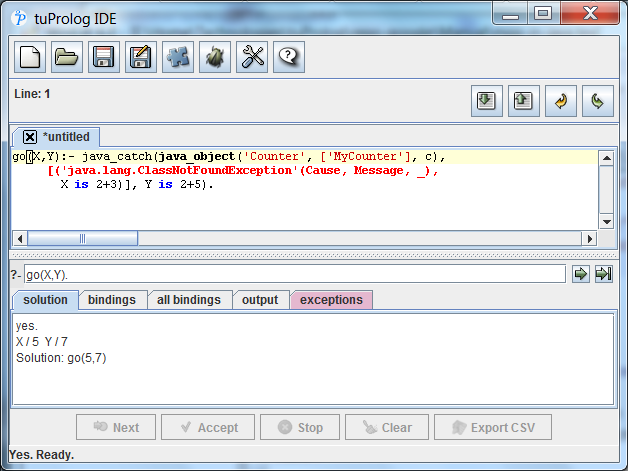
\includegraphics[width=7cm]{images/exceptions1a}
  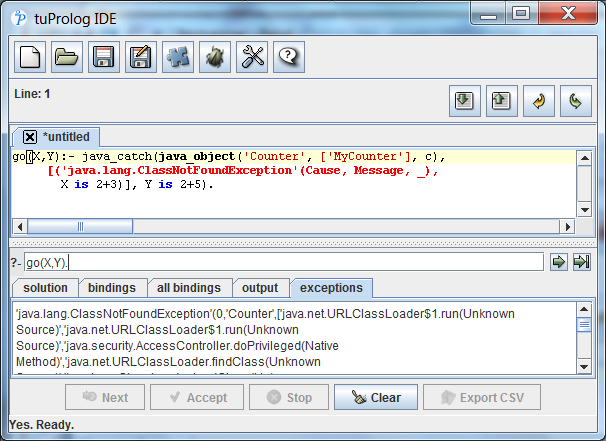
\includegraphics[width=7cm]{images/exceptions1b}
  \caption{Catching the Java exceptions of Example 1 in the \tuprolog{} GUI.
  \textit{Top:} the solutions tab.
  \textit{Bottom:} details of the exception in the exception tab (see the \texttt{Cause} variable bound to \texttt{0} and the \texttt{Msg} variable bound to \texttt{'Counter'}; the other details map onto the anonymous variable \texttt{\_}). }\label{fig:exceptions1}
\end{figure}


\medskip\noindent
\textit{\textbf{Example 2:} execution must fail if an exception is raised during the execution of a goal and no matching \texttt{java\_catch/3} is found.}
\begin{verbatim}
 ?- java_catch(java_object('Counter', ['MyCounter'], c),
      [('java.lang.Exception'(Cause, Message, _), true)], true)).
\end{verbatim}

Answer: \texttt{ no.}

\noindent In the \tuprolog{} GUI, a failed exception not only results into a "No" answer as in other Prolog systems (that answer is shown in the status bar at the bottom of the window: it also causes the \textit{halt} message to appear in the Solutions tab (Figure \ref{fig:exceptions2}).

\begin{figure}
  \centering
  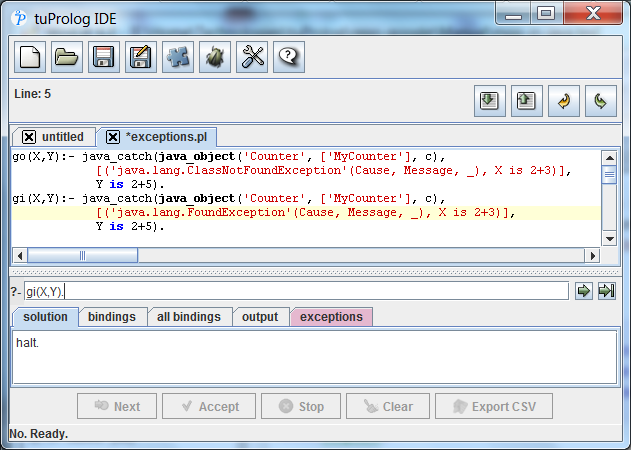
\includegraphics[width=7cm]{images/exceptions2}
  \caption{A failed exception in the \tuprolog{} GUI: the \texttt{No} answer in the status bar and the \textit{halt} message in the Solutions tab.}
  \label{fig:exceptions2}
\end{figure}


\medskip\noindent
\textit{\textbf{Example 3:} \texttt{java\_catch/3} must fail if the handler is false.}
\begin{verbatim}
 ?- java_catch(java_object('Counter', ['MyCounter'], c),
      [('java.lang.Exception'(Cause, Message, _), false)], true)).
\end{verbatim}

Answer: \texttt{ no.}

\medskip\noindent
\textit{\textbf{Example 4:} \texttt{java\_catch/3} must fail also if an exception is raised during the execution of the handler.}
\begin{verbatim}
 ?- java_catch(java_object('Counter', ['MyCounter'], c),
      [('java.lang.ClassNotFoundException'(Cause, Message, _),
        java_object('Counter', ['MyCounter'], c))], true).
\end{verbatim}

Answer: \texttt{ no.}

\medskip\noindent
\textit{\textbf{Example 5:} the \textit{\texttt{Finally}} must be executed also in case of success of the goal.}
\begin{verbatim}
 ?- java_catch(java_object('java.util.ArrayList', [], l),
       [E, true], X is 2+3).
\end{verbatim}

Answer: \texttt{ yes.}

Substitutions: \texttt{X/5}.

\medskip\noindent
\textit{\textbf{Example 6:} the \textit{\texttt{Handler}} to be executed must be the proper one among those available in the handlers' list.}
\begin{verbatim}
 ?- java_catch(java_object('Counter', ['MyCounter'], c),
     [('java.lang.Exception'(Cause, Message, _), X is 2+3),
      ('java.lang.ClassNotFoundException'(Cause, Message, _), Y is 3+5)],
      true).
\end{verbatim}

Answer: \texttt{ yes.}

Substitutions: \texttt{Cause/0}, \texttt{Message/'Counter'}, \texttt{Y/8}.

%-----------------------------------------------------------------------
\newpage
\section{Using Prolog from Java: \textit{the Java API}}
\label{sec:java-api}
%-----------------------------------------------------------------------

The \tuprolog{} Java API provides a complete support for exploiting Prolog engines from Java: its only requirement is the presence of \texttt{tuprolog.jar} (or the more complete \texttt{2p.jar}) in the Java project's class path.
The API defines a namespace (\texttt{alice.tuprolog}) and classes to enable the definition in Java of suitable objects representing Prolog entities (terms, atoms, lists, variables, numbers, etc, but also Prolog engines, libraries and theories), and use them to submit queries and get the results back in Java, thus effectively supporting multi-paradigm, multi-language programming.

%-----------------------------
\subsection{A Taxonomy of Prolog types in Java}
\label{ssec:java-api-types}
%-----------------------------

Prolog types are mapped onto suitable Java classes, organized into the taxonomy shown in Figure \ref{fig:term-taxonomy} and summarized in Table \ref{tab:prolog-java-type-mapping} on page \pageref{tab:prolog-java-type-mapping}.

\begin{figure}[b]
    \setlength{\unitlength}{1mm}
    \begin{picture}(80,27){\scriptsize
        \put(30,11){\framebox(13,5){Term}}
        %
        \put(50, 3){\framebox(13,5){Struct}}
        \put(50,11){\framebox(13,5){Number}}
        \put(50,19){\framebox(13,5){Var}}
        %
        \put(70, 3){\framebox(13,5){Int}}
        \put(90, 3){\framebox(13,5){Long}}
        \put(70,19){\framebox(13,5){Float}}
        \put(90,19){\framebox(13,5){Double}}

        \put(43,13.5){\line(1,0){6.5}}
        \put(63,13.5){\line(1,0){24}}
        %
        \put(67,21){\line(1,0){3}}
        \put(67,5.5){\line(1,0){3}}
        \put(67,21){\line(0,-1){15.5}}
        %
        \put(47,21){\line(1,0){3}}
        \put(47,5.5){\line(1,0){3}}
        \put(47,21){\line(0,-1){15.5}}
        %
        \put(87,21){\line(1,0){3}}
        \put(87,5.5){\line(1,0){3}}
        \put(87,21){\line(0,-1){15.5}}
    }
    \end{picture}
    \caption{Prolog entities as a taxonomy of Java classes.}
    \label{fig:term-taxonomy}
\end{figure}

\texttt{Term} is the root abstract class, providing common services such as term unification, term parsing, term copying, etc.; its subclasses distinguish among untyped terms (structures), numbers, and variables.

\texttt{Struct} objects are characterized by a functor name (a Java string) and
a list of arguments, which are \texttt{Term}s themselves and can be
individually retrieved via the \texttt{getTerm} method.

Atoms are a special case of \texttt{Struct} with no arguments; among these, the \texttt{true} and \texttt{false} atom constants are used to represent the Java boolean values.
Atoms are also used to map Java \texttt{char}s and strings: when converted back to Java, however, atoms are always mapped into Java \texttt{String}s.

Prolog lists are another special case of \texttt{Struct}, built from either
two \texttt{Term}s (the list head and tail) or an array of \texttt{Term}s; by
convention, the default constructor builds the empty list.

The \texttt{Number} subtree includes classes for numeric types, and offers methods such as \texttt{intValue}, \texttt{longValue}, etc. to retrieve the number value as the corresponding primitive Java value.
As discussed above, in the Prolog-to-Java direction, Prolog integers are always mapped onto \texttt{Int} instances and Prolog reals onto \texttt{Double} instances, while in the Java-to-Prolog direction any of the numeric Java types are accepted (including \texttt{short}, \texttt{byte} and \texttt{float}) for mapping onto Prolog numbers.
In particular, Java \texttt{int} and \texttt{long} values are mapped onto suitable \texttt{Int} and \texttt{Long} instances of the \tuprolog{} taxonomy, respectively, while \texttt{byte} and \texttt{short} Java types are mapped into \texttt{Int} instances.
Please note that to avoid possible name clashes between \tuprolog{} types and Java wrapper classes (e.g. \texttt{alice.tuprolog.Long} and \texttt{java.lang.Long}), it is often necessary to use the fully qualified class name to denote \tuprolog{} numeric classes.

\texttt{Var} represents Prolog variables, built from a Java string representing the variable name: as prescribed by the Prolog rules, the name must start either with a capital letter, or with an underscore.
The default constructor builds the anonymous Prolog variable \texttt{\_}, mapped onto the Java \texttt{null} value.

Table \ref{tab:creating-prolog-terms-in-java} on page \pageref{tab:creating-prolog-terms-in-java} shows how to manipulate Prolog entities (variables, terms, structures, lists, atoms..) from a Java program: variable creation (lines 1 and 10), list construction (lines 2--4), term construction for \texttt{p(a,5)} and \texttt{p(X,Y)} (lines 5--6), and term unification (lines 7--14) (the latter requires a Prolog engine as a mediator, to handle execution contexts and inner variables).

It is worth noting that, in general, two different \texttt{Var} objects with the same Java name \textit{do not} refer to the same Prolog variable, unless they occur in the same term.
So, multiple occurrences of \texttt{new Var("Y")} outside the same term refer to two distinct variables, as if they were renamed \texttt{Y1} and \texttt{Y2}.
%
To refer to the same Prolog variable twice, just use the same Java identifier (see \texttt{varY} in lines 1, 3, 12) instead of creating a new variable.

The only exception is the case when the homonymous variables occur in the same term, as in the \texttt{q(Y,Y)} term in line 15: then, they will refer to the same variable, \textit{but only after the term has been resolved}.
In fact, new terms are always built in an `unresolved' form, that does not analyze the term variables: the proof is the \textit{\texttt{false}} output of line 16.
Variables are taken into consideration later, when the term is either explicitly resolved via \texttt{resolveTerm} (line 17), or is involved in a \texttt{match} or \texttt{unify}\footnote{\texttt{q(Y,Y)} is unified here with the Prolog anonymous variable, so success is granted.} operation with another term (lines 18-19), as proved by the \textit{\texttt{true}} output of line 20.

\begin{table}[h]
    \small
    \begin{center}{\tt
    \begin{tabular}{p{13cm}}\hline\\
    \mbox{~~~}import alice.tuprolog.*;\\
    \mbox{~~~}\ldots\\
    \mbox{1~~}Var varX = new Var("X"), varY = new Var("Y"); \\
    \mbox{2~~}Struct atomP = new Struct("p");\\
    \mbox{3~~}Struct list = new Struct(atomP, varY);~~~~~~~\textit{// should be [p|Y]}\\
    \mbox{4~~}System.out.println(list);~~~~~~~~~~~~~~\textit{// prints the list [p|Y]}\\
    \mbox{5~~}Struct fact = new Struct("p", new Struct("a"), new Int(5));\\
    \mbox{6~~}Struct goal = new Struct("p", varX, new Var("Z"));\\
    \mbox{7~~}Prolog engine = new Prolog();\\
    \mbox{8~~}boolean res = goal.unify(engine,fact);~~~~~\textit{// should be X/a, Y/5}\\
    \mbox{9~~}System.out.println(goal);~~~~~\textit{// prints the unified term p(a,5)}\\
    \mbox{10~}System.out.println(varX);~~~~~\textit{// prints the variable binding X/a}\\
    \mbox{11~}Var varW = new Var("W");\\
    \mbox{12~}res = varW.unify(engine,varY);~~~~~~~~~~~~~~~~~~\textit{// should be Z=Y}\\
    \mbox{13~}System.out.println(varY);~~\textit{// prints just Y, since it is unbound}\\
    \mbox{14~}System.out.println(varW);~~\textit{// prints the variable binding W / Y}\\
    \mbox{15~}Struct st = Struct("q", new Var("Y"), new Var("Y"));~\textit{// unresolved}\\
    \mbox{16~}System.out.println(st.getArg(0)==st.getArg(1));~~\textit{// prints false}\\
    \mbox{17~}st.resolveTerm();~~~~~~~~~~~~~~~~~~~\textit{// now the term is resolved}\\
    \mbox{18~}~~\textit{alternatively:} res = st.match(new Struct());\\
    \mbox{19~}~~\textit{alternatively:} res = st.unify(engine, new Struct());\\
    \mbox{20~}System.out.println(st.getArg(0)==st.getArg(1));~~\textit{// prints true}\\
    \\\hline
    \end{tabular}}
    \end{center}
    \caption{Manipulating Prolog entities from Java.}
    \label{tab:creating-prolog-terms-in-java}
\end{table}

\subsubsection{Further notes about \texttt{Term}s}

The \texttt{Term} class is the home of several general-purpose services, used throughout \tuprolog{}; in particular:

\begin{itemize}
\item the static \texttt{parse} and \texttt{createTerm} methods provides a quick way  to get a term from its string representation;

\item the \texttt{match} and \texttt{unify} methods respectively check for term matching (but performing no actual unification) and unify the given term with the provided one; as anticipated above, the latter requires a \texttt{Prolog} argument, to be used as a mediator during (nested) unification;
    Instead, the matching test is performed outside any demonstration context.

\item the \texttt{equals} method compares terms with the same semantics of the method \texttt{isEqual}, which follows the Prolog comparison semantics.

\item the \texttt{getTerm} method returns the referred term, following variable bindings---that is, if the target term is a bound variable, the term bound to the variable (not the variable itself) is returned.
\end{itemize}


%-----------------------------
\subsection{Prolog engines, theories and libraries}
\label{ssec:java-api-engine-solveinfo}
%-----------------------------

The \tuprolog{} engine is made accessible in Java via the \texttt{Prolog} class: so, adding intelligence to a Java program is as easy as creating \texttt{Prolog} instance(s), configure it (them) as needed, and perform the desired queries. Query results are expressed as an instance of the \texttt{SolveInfo} helper class.
Table \ref{tab:engine-interface} reports the public interface of these classes.

\begin{table}
    \renewcommand\arraystretch{1}
    \begin{center}{\tt
    \begin{tabular}{p{14cm}}\hline\\
    public class Prolog implements Serializable \{\\
    ~~\ldots\\
    ~~public void setTheory(Theory t) throws InvalidTheoryException \{\ldots\}\\
    ~~public void addTheory(Theory t) throws InvalidTheoryException \{\ldots\}\\
    ~~public Theory getTheory() \{\ldots\}\\
    ~~public Library loadLibrary(String name)\\
    ~~~~~~~~~~~~~~~~~~~~~~~~~~~~~~~~~throws InvalidLibraryException \{\ldots\}\\
    ~~public void~unloadLibrary(String name)\\
    ~~~~~~~~~~~~~~~~~~~~~~~~~~~~~~~~~throws InvalidLibraryException \{\ldots\}\\
    ~~public Library getLibrary(String name) \{\ldots\}\\
    ~~public SolveInfo solve(Term goal) \{\ldots\}\\
    ~~public SolveInfo solve(String goalAsString)\\
    ~~~~~~~~~~~~~~~~~~~~~~~~~~~~~~throws MalformedGoalException \{\ldots\}\\
    ~~public boolean hasOpenAlternatives() \{\ldots\}\\
    ~~public SolveInfo solveNext()~throws NoMoreSolutionException \{\ldots\}\\
    ~~public boolean isHalted() \{\ldots\}\\
    \}\\
    \\\hline\\
    public class SolveInfo implements Serializable \{\\
    ~~public boolean isSuccess() \{\ldots\}\\
    ~~public Substitution getSubstitution()\\
    ~~~~~~~~~~~~~~~~~~~~~~~~~~~~~~throws NoSolutionException \{\ldots\}\\
    ~~public Term getTerm() throws UnknownVarException \{\ldots\}\\
    ~~public Term  getSolution() throws NoSolutionException \{\ldots\}\\
    \}\\
    \\\hline
    \end{tabular}}
    \end{center}
    %
    \caption{Classes for interacting with \tuprolog{} engines.}
    \label{tab:engine-interface}
\end{table}

A Prolog engine is built by one of \texttt{Prolog} constructors: the default constructor builds a default engine, with the default set of \tuprolog{} libraries loaded, and no user theory. In most cases, this is all you need to bring the power of Logic programming to Java.
%
However, libraries can be loaded and unloaded dynamically at any time after the engine creation, via the \texttt{loadLibrary} and \texttt{unloadLibrary} methods: their argument is the name of the library. If the library is invalid, an exception is raised.
%
A reference to a loaded library can be obtained via the \texttt{getLibrary} method, which returns a reference to the abstract \texttt{Library} class.
%
Such a reference can be used to operate on the library, as discussed below.

The user theory can either be set from scratch via the \texttt{setTheory} method, which overwrites any previous theory, or be built incrementally, adding new clauses to the existing theory via the \texttt{addTheory} method: both take a \texttt{Theory} as their argument. This theory can be built in several ways---from an input stream, from a string, or from a clause list (represented as a \texttt{Struct} object).
%
The current theory can be retrieved via the \texttt{getTheory} method.

Goal resolution is handled via three methods: \texttt{solve}, \texttt{solveNext}, and
\texttt{hasOpenAlternatives}.
%
\texttt{solve} and \texttt{solveNext} take as their argument a \texttt{Struct} representing the goal, and return a \texttt{SolveInfo} which encapsulates the result information (success or failure, solution, variable bindings, etc).
%
An overloaded version of \texttt{solve} takes a string argument representing the text of the goal, embedding its parsing.
%
Both \texttt{solve} and \texttt{solveNext} raise the proper exceptions when needed.


\subsubsection{Further notes about \texttt{Prolog} engines}

The \texttt{Prolog} class is the home of \tuprolog{} engines, so some further information is opportune about its behavior in particular contexts:

\begin{itemize}
\item engines support natively some \emph{directives}, that can be defined by means of the \texttt{:-/1} predicate in theory specification.
    Directives are used to specify properties of clauses and engines (\texttt{solve/1}, \texttt{initialization/1}, \texttt{set\_prolog\_flag/1}, \texttt{load\_library/1}, \texttt{consult/1}), format and syntax of read-terms (\texttt{op/3}, \texttt{char\_conversion/2}).

\item engines also support the dynamic definition and management of \emph{flags} (or property), used to describe some aspects of libraries and their built-ins.
    A flag is identified by a name (an alphanumeric atom), a list of possible values, a default value and a boolean value specifying if the flag value can be modified.

\item engines are thread-safe.

\item engines have no (static) dependencies with each other, can be created  independently on the same Java virtual machine, are very lightweight, and can be serialized.
    This is true also for engines with the standard libraries pre-loaded: obviously, if other libraries are loaded, these must be serializable, too, for the engine to remain serializable.
\end{itemize}

%-------------------------------------------------------
\subsection{Examples}
\label{ssec:java-api-examples}
%-------------------------------------------------------

For the sake of concreteness, some examples of use of the \tuprolog{} Java API are now discussed.

%--------------
\subsubsection{Appending lists}
%--------------

\begin{table}
\textit{Basic version:}
{\small{
\begin{verbatim}
    import alice.tuprolog.*;

    public class Example1 {
        public static void main(String[] args) throws Exception {
            Prolog engine = new Prolog();
            SolveInfo info = engine.solve("append([1],[2,3],X).");
            System.out.println(info.getSolution());
        }
    }
\end{verbatim}
}}
\textit{Variant:}
{\small{
\begin{verbatim}
    import alice.tuprolog.*;

    public class Example2 {
        public static void main(String[] args) throws Exception {
            Prolog engine = new Prolog();
            SolveInfo info = engine.solve("append(X,Y,[1,2]).");
            while (info.isSuccess()) {
                System.out.println("solution: " + info.getSolution() +
                                   " - bindings: " + info);
                if (engine.hasOpenAlternatives()) {
                    info = engine.solveNext();
                } else {
                    break;
                }
            }
        }
    }
\end{verbatim}
}}
\caption{The list appending example.}
\label{tab:java-api-example1}
\end{table}

In this first example (see Table \ref{tab:java-api-example1}, \textit{top}), a \tuprolog{} engine is asked to solve a trivial list append goal, provided in textual form.\footnote{The \texttt{append/3} predicate is included in BasicLibrary, which is part of the engine default configuration.}
%
The program must be compiled and executed normally, taking care of including the \tuprolog{} JAR in the classpath:

\texttt{javac -cp tuprolog.jar;. Example1.java}\\
\texttt{\mbox{~~~}java~ -cp tuprolog.jar;. Example1}

\noindent The string \texttt{append([1],[2,3],[1,2,3])} should be displayed.

\medskip

\noindent Table \ref{tab:java-api-example1}, \textit{bottom} shows a variant where all the solutions are displayed, with their variable bindings. The output should be as follows:

\begin{verbatim}
solution: append([],[1,2],[1,2]) - bindings: X/[]    Y/[1,2]
solution: append([1],[2],[1,2])  - bindings: X/[1]   Y/[2]
solution: append([1,2],[],[1,2]) - bindings: X/[1,2] Y/[]
\end{verbatim}

%--------------
\subsubsection{A console-based Prolog interpreter}
%--------------

\begin{table}
    \small
    \begin{center}{\tt
    \begin{tabular}{p{14cm}}\hline\\
    import alice.tuprolog.*;\\
    import java.io.*;\\
    \\
    public class ConsoleInterpreter  \{\\
    ~public static void main (String args[]) throws Exception \{\\
    ~~Prolog engine=new Prolog();\\
    ~~if (args.length>0)\\
    ~~~~~~engine.setTheory(new Theory(new FileInputStream(args[0])));\\
    ~~BufferedReader stdin =\\
    ~~~~~~new BufferedReader(new InputStreamReader(System.in));\\
    ~~while (true) \{ \textit{~~~~// interpreter main loop} \\
    ~~~String goal;\\
    ~~~do \{ System.out.print("?- "); goal=stdin.readLine();\\
    ~~~\} while (goal.equals(""));\\
    ~~~try \{\\
    ~~~~SolveInfo info = engine.solve(goal);\\
    ~~~~if (engine.isHalted()) break;\\
    ~~~~else if (!info.isSuccess()) System.out.println("no.");\\
    ~~~~else if (!engine.hasOpenAlternatives()) \{\\
    ~~~~~~System.out.println(info);\\
    ~~~~\} else \{ \textit{// main case}\\
    ~~~~~~System.out.println(info + " ?");\\
    ~~~~~~String answer = stdin.readLine();\\
    ~~~~~~while (answer.equals(";") \&\& engine.hasOpenAlternatives())
    \{\\
    ~~~~~~~~info = engine.solveNext();\\
    ~~~~~~~~if (!info.isSuccess()) \{ System.out.println("no."); break; \}\\
    ~~~~~~~~else \{\\
    ~~~~~~~~~~~~~~~System.out.println(info + " ?");\\
    ~~~~~~~~~~~~~~~answer = stdin.readLine();\\
    ~~~~~~~~\} \textit{// endif}\\
    ~~~~~~\} \textit{// endwhile}\\
    ~~~~~~if (answer.equals(";") \&\& !engine.hasOpenAlternatives())\\
    ~~~~~~~~~~System.out.println("no.");\\
    ~~~~\} \textit{// end main case}\\
    ~~~\} catch (MalformedGoalException ex) \{\\
    ~~~~~~~~~~System.err.println("syntax error.");\\
    ~~~\} \textit{// end try}\\
    ~~\} \textit{// end main loop}\\
    ~~if (args.length>1) \{\\
    ~~~Theory curTh = engine.getTheory(); \textit{// save current theory to file}\\
    ~~~new
    FileOutputStream(args[1]).write(curTh.toString().getBytes());\\
    ~~\}\\
    ~\}\\
    \}\\
    \\\hline
    \end{tabular}}
    \end{center}
    \caption{A simple console-based Prolog interpreter.}
    \label{tab:console-sample}
\end{table}

As a final example, Table \ref{tab:console-sample} shows a console-based Prolog interpreter: first a \tuprolog{} engine is created and initialized with a theory built from a text file (whose name is taken from the command line), then a classic read/solve loop is started.
%
For each goal read from the standard input, the \texttt{solve} method is invoked: if multiple solutions exist, the \texttt{solveNext} makes it possible to explore the open
alternatives.
%
The loop ends when the \texttt{halt} predicate is typed in: the current theory is then saved to file (if any has been specified).
Figure \ref{fig:console-interpreter} shows a sample session with this interpreter.

\begin{figure}
  \centering
  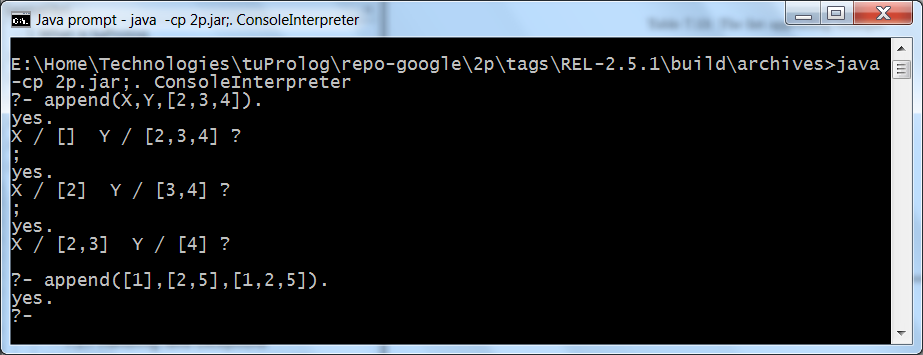
\includegraphics[width=12cm]{images/console-interpreter}
  \caption{A sample session with the Console-based Interpreter.}
  \label{fig:console-interpreter}
\end{figure}

%-----------------------------------------------------------------------
\subsection{Registering object bindings}
\label{ssec:register(Java)}
%-----------------------------------------------------------------------

The \texttt{register} function, already discussed in Section \ref{sssec:register(prolog)} on page \pageref{sssec:register(prolog)} for what concerns the Prolog side, is also available on the Java side, where its `global' effect is more natural and coherent with the imperative paradigm than it is on the Prolog side.

Its purpose is to permanently associate an existing Java object \texttt{\textit{obj}} to a Prolog identifier \texttt{\textit{ObjectRef}}, as follows:\\

\texttt{boolean register(Struct \textit{ObjectRef}, Object \textit{obj})\\
    \mbox{~~~~~~~~~~~}throws InvalidObjectIdException;}\\

\noindent where \texttt{\textit{ObjectRef}} is a ground term (otherwise an \texttt{InvalidObjectIdException} exception is raised) representing the Java object
\texttt{\textit{obj}} in the context of \texttt{JavaLibrary}'s predicates.
The function returns \texttt{false} if that object is already registered under a different \texttt{\textit{ObjectRef}}.

As an example, let us suppose that we want to permanently bind the Prolog atom \texttt{stdout} to the Java (static) object \texttt{System.out}, so that Java-based printing can be done from the Prolog side without having to retrieve and re-bind the \texttt{out} object every time, as we did in Table \ref{tab:javalibrary-counter-example} on page \pageref{tab:javalibrary-counter-example} (reported again below for convenience):

\begin{verbatim}
  class('java.lang.System') . out <- get(Out),
  Out <- println(...),
\end{verbatim}

\noindent To bind \texttt{System.out} permanently to \texttt{stdout} (within the scope of the \tuprolog{} engine \texttt{engine}), we can register it as follows:

{\small
\begin{verbatim}
  Prolog engine = new Prolog();
  Library lib = engine.getLibrary("alice.tuprolog.lib.JavaLibrary");
  ((JavaLibrary)lib).register(new Struct("stdout"), System.out);
\end{verbatim}}

\noindent An explicit downcast to \texttt{JavaLibrary} is needed to convert the returned reference type \texttt{Library}, since \texttt{register} is defined in \texttt{JavaLibrary} only.
%
Now, a Prolog theory loaded into this \texttt{engine} can contain a phrase like:
%
\begin{verbatim}
  stdout <- println('What a nice message!')
\end{verbatim}
%
which uses \texttt{stdout} directly as a target for the \texttt{println} method.

A small yet complete sample program is shown in Table \ref{tab:registering-stdout-example}, where the theory loaded into the \texttt{engine} prints the standard greetings message.

\begin{table}[h]
{\small
\begin{verbatim}
  import alice.tuprolog.*;
  import alice.tuprolog.lib.*;

  public class StdoutExample {
    public static void main(String[] args) throws Exception {
    Prolog engine = new Prolog();
    Library lib = engine.getLibrary("alice.tuprolog.lib.JavaLibrary");
    ((JavaLibrary)lib).register(new Struct("stdout"), System.out);
    engine.setTheory(new Theory(
        ":-solve(go). \n go:- stdout <- println('hello!')."));
    }
 }
\end{verbatim}}
\caption{A program registering \texttt{stdout} for \texttt{System.out}. As an alternative to \texttt{getLibrary}, \texttt{loadLibrary} could have been used---if the library is already loaded, its behavior is identical to \texttt{getLibrary}'s.
%
Also, the fully qualified class name \texttt{"alice.tuprolog.lib.JavaLibrary"} is needed in \texttt{getLibrary} only because \texttt{JavaLibrary} does \textit{not} define a short library name (see Section \ref{ssec:library-name} for details): otherwise, the shorter name could have been used.}
\label{tab:registering-stdout-example}
\end{table}

%-------------------------------------------------------
\subsection{Capturing the Prolog output in Java}
\label{ssec:capturing-output}
%-------------------------------------------------------

If a \tuprolog{} engine is used in a Java application, the output performed by Prolog \texttt{write} predicates (more generally, of any predicate writing on the Prolog console) is not available in Java: printed messages are not captured, nor are they retrievable by any of the \tuprolog{} Java API methods.
%
The only way to `capture' somehow the output of the Prolog engine is to write it to a file or store it in a Prolog term---just two variants of the same inconvenience.

Yet, this feature can be added in a non-intrusive way, thanks to \tuprolog{}'s extensible architecture, by simply overriding the \texttt{onOutput} method used internally by the engine to handle the write requests.\footnote{This approach was originally suggested by Josh Guzman in the \tuprolog{} users' forum.}
All is needed is to redefine this method so as to capture the output message and store it conveniently---for instance, into a suitable \texttt{String} of the Java application (here, \texttt{finalResult}), as follows:

\begin{verbatim}
  engine.addOutputListener(new OutputListener() {
    @Override
    public void onOutput(OutputEvent e) {
      finalResult += e.getMsg();
    }
  });
\end{verbatim}

\noindent This elegant approach does not modify the \tuprolog{} code in any way: it just adds listener to an existing event, extending the service non-intrusively.
%
A full example of this technique is reported in Table
\ref{tab:capturing-output-complete} on page \pageref{tab:capturing-output-complete}, together with the corresponding build process and execution.

\begin{table}[h]
{\small
\begin{verbatim}
  import alice.tuprolog.*;
  import alice.tuprolog.lib.*;
  import alice.tuprolog.event.*;

  public class OnOutputExample {
    static String finalResult = "";
    public static void main(String[] args) throws Exception {
      Prolog engine = new Prolog();
      engine.addOutputListener(new OutputListener() {
          @Override
          public void onOutput(OutputEvent e) {
            finalResult += e.getMsg();
          }
      });
      Term goal = Term.createTerm("write('Hello world!')");
      SolveInfo res = engine.solve(goal);
      res = engine.solve("write('Hello everybody!'), nl.");
      System.out.println("OUTPUT: " + finalResult);
    }
  }
\end{verbatim}}
  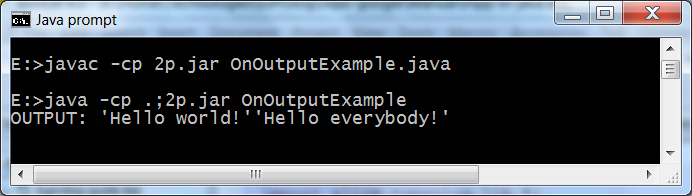
\includegraphics[width=12cm]{images/onOutput}
\caption{Capturing the Prolog output from Java: a complete example.}
\label{tab:capturing-output-complete}
\end{table}

%-----------------------------------------------------------------------
\section{Augmenting Prolog via Java:\\developing new libraries}
\label{sec:howto-develop-libraries}
%-----------------------------------------------------------------------

So far, the two first dimensions of \tuprolog{}'s support to multi-paradigm, multi-language programming have been explored, that enable a language (and the corresponding paradigm) to be used from the other.
The two further dimensions concerns \textit{augmenting} the language instead---that is, exploiting a language (and a paradigm) to increase the other.

In this section the focus is on augmenting Prolog from Java, exploiting the latter\footnote{%
 Other languages may be used indirectly, via JNI (JavaNative Interface}
to increase the first by developing new \tuprolog{} libraries; the next Section (\ref{sec:p@j}) will focus on the opposite direction, exploiting Prolog to augment Java via the so-called \textit{P@J} framework.

Moreover, although \tuprolog{} libraries are expressed in Java, they are not required to
be fully implemented in this language.
%
In fact, Java-only libraries are the simplest case, but hybrid Java + Prolog libraries are also possible, where a Prolog theory is embedded into a Java string so that the
two parts cooperate to define the overall library behavior.
This opens further interesting perspectives, that will be discussed below.

%---------------------------------------------------------------
\subsection{Syntactic conventions}
\label{ssec:library-syntax}
%---------------------------------------------------------------
Each library must extend the base abstract class \texttt{alice.tuprolog.Library} and define new \textit{predicates} and/or \textit{evaluable functors} and/or \textit{directives} in the form of methods, following a simple signature convention.

\noindent Predicates must adhere to the signature:\\

{\small\tt
%    public boolean <\textit{pred name}>\_<\textit{N}>(\textit{T1} arg1, \textit{T2} arg2, ...,\textit{Tn} argN)
    public boolean <\textit{pred name}>\_<\textit{N}>(\\
    \mbox{~~~~~~~~~~~~}<?~extends~Term> arg1, ..., <?~extends~Term> argN)
}\\

\noindent while evaluable functors must follow the form:\\

{\small\tt
%    public Term <\textit{eval funct name}>\_<\textit{N}>(\textit{T1} arg1, \textit{T2} arg2, ...,\textit{Tn} argN)
    public Term <\textit{eval funct name}>\_<\textit{N}>(\\
    \mbox{~~~~~~~~~~~~}<?~extends~Term> arg1, ..., <?~extends~Term> argN)
}\\

\noindent and directives must be provided with the signature:\\

{\small\tt
%    public void <\textit{dir name}>\_<\textit{N}>(\textit{T1} arg1, \textit{T2} arg2, ..., \textit{Tn} argN)
    public void <\textit{dir name}>\_<\textit{N}>(\\
    \mbox{~~~~~~~~~~~~}<?~extends~Term> arg1, ..., <?~extends~Term> argN)
}\\

\noindent where \textit{arg1}, ... \textit{argN} are \texttt{Term}s\footnote{%
 Please refer to Table \ref{fig:term-taxonomy} on page \pageref{fig:term-taxonomy} for the full Term taxonomy.}
that represent the actual arguments passed to the predicate (functor, directive).

\begin{table}
    \begin{center}{\small\tt
    \begin{tabular}{p{12cm}}
     \hline\\
    import alice.tuprolog.*;\\
    public class TestLibrary extends Library \{\\
    \\
    ~~\textit{// functor sum(A,B)}\\
    ~~public Term sum\_2(Number arg0, Number arg1)\{\\
    ~~~~float  n0 = arg0.floatValue();\\
    ~~~~float  n1 = arg1.floatValue();\\
    ~~~~return new Float(n0+n1);\\
    ~~\}\\
    \\
    ~~\textit{// predicate println(Message)}\\
    ~~public boolean println\_1(Term arg)\{\\
    ~~~~System.out.println(arg);\\
    ~~~~return true;\\
    ~~\}\\
    \\
    ~~\textit{// predicate invert(StringIn,StringOut)}\\
    ~~public boolean invert\_2(Term in, Var out)\{\\
    ~~~~String s1 = null, s2 = "";\\
	~~~~if (in instanceof Var) s1 = in.getTerm().toString();\\
	~~~~else s1 = in.toString();\\
	~~~~for(int i=0; i<s1.length(); i++)\{\\
	~~~~~~char ch = s1.charAt(i);\\
	~~~~~~if (ch=='$\backslash$'') continue;\\
	~~~~~~if (Character.isUpperCase(ch))\\
	~~~~~~~~s2 += Character.toLowerCase(ch);\\
	~~~~~~else\\
	~~~~~~~~s2 += Character.toUpperCase(ch);\\
	~~~~\}\\
	~~~~return out.unify(getEngine(),new Struct(s2));\\
    ~~\}\\
    \\\hline
    \end{tabular}
    }\end{center}
    \caption{Definition of a \tuprolog{} library in Java.}
    \label{tab:TestLibrary}
\end{table}

Table \ref{tab:TestLibrary} shows a library defining an evaluable functor (\texttt{sum/2}) and two predicates (\texttt{println/1}, \texttt{invert/2}).
%
The Java method \texttt{sum\_2}, which implements the evaluable functor \texttt{sum/2}, is passed two \texttt{Number} terms (5 and 6) which are then used (via \texttt{getTerm}) to retrieve the two (float) arguments to be summed.
%
In the same way, method \texttt{println\_1}, which implements the predicate \texttt{println/1}, receives \texttt{N} as \texttt{arg}, and retrieves its actual value via \texttt{getTerm}: since this is a predicate, a boolean value is returned, representing success or failure (\texttt{true} = success in this case).
%
Analogous considerations hold for \texttt{invert/2}, whose input argument is first type-checked to handle variables appropriately (the related bound term must be retrieved), then the input term is scanned to build the output string, which is finally unified with the output variable.

A test Java program, which loads this library and tests its predicates, is shown in Table \ref{tab:TestLibrary-Main}.
%
The program creates the Prolog engine, loads \texttt{TestLibrary} (checking that it was actually loaded), defines a theory containing the Prolog test code and sets it into the engine: then, the three test goals are solved in sequence.
%
The printed output is reported in the bottom part of the Table.
The \texttt{\textit{Name} / \textit{Value}} format is the \tuprolog{}'s default for variables, and is \texttt{\textit{Name}} is composed of the Prolog variable name (\texttt{N}, \texttt{S}, etc.) and of a unique internal identifier.
%
As expected, \texttt{N} is bound to \texttt{11}, \texttt{S} to \texttt{abcd}, the \texttt{X} and \texttt{Z} pair to \texttt{ab}/\texttt{'AB'}, \texttt{bc}/\texttt{'BC'} and \texttt{uk}/\texttt{'UK'}, respectively.

\begin{table}
    \begin{center}{\small\tt
    \begin{tabular}{p{12cm}}
     \hline\\
    import alice.tuprolog.*;\\
    import alice.tuprolog.lib.*;\\
    \\
    public class TestLibraryMain \{\\
    ~~public static void main(String[] args) throws Exception \{\\
	~~~~Prolog engine = new Prolog();\\
	~~~~Library lib1 = engine.loadLibrary("TestLibrary");\\
	~~~~System.out.println(\\
	~~~~~~~~"Lib1 " + (lib1==null ? "NOT " : " ") + "LOADED");\\
	~~~~Theory testTheory = new Theory(\\
	~~~~~~~~"test1 :- N is sum(5,6), println(N).$\backslash$n" +\\
	~~~~~~~~"test2 :- invert('ABCD',S), println(S).$\backslash$n" +\\
	~~~~~~~~"test3 :- name(X), println(X)," +\\
	~~~~~~~~~~~~~~~~~"invert(X,Z), println(Z), fail.$\backslash$n" +\\
	~~~~~~~~"name(ab).$\backslash$n name(bc).$\backslash$n name(uk).$\backslash$n");\\
	~~~~engine.setTheory(testTheory);\\
	~~~~SolveInfo res = engine.solve("test1.");\\
	~~~~res = engine.solve("test2.");\\
	~~~~res = engine.solve("test3.");\\
	~~\}\\
    \}\\
    \\
    \textrm{\textit{OUTPUT PRINTED:}}\\
    Lib1  LOADED\\
    N\_e2 / 11.0\\
    S\_e2 / abcd\\
    X\_e11 / ab\\
    Z\_e12 / 'AB'\\
    X\_e13 / bc\\
    Z\_e14 / 'BC'\\
    X\_e15 / uk\\
    Z\_e17 / 'UK'\\
    \\\hline
    \end{tabular}
    }\end{center}
    \caption{A test program for the library defined in Table \ref{tab:TestLibrary} \textit{(top)} and the corresponding output \textit{(bottom)}.}
    \label{tab:TestLibrary-Main}
\end{table}

Alternatively, the same theory can be loaded from the Prolog side, via the \texttt{load\_library} predicate (Figure \ref{fig:testlibrary3}, \textit{top}) or via the library manager tool in the GUI (Figure \ref{fig:testlibrary1}).

Please note that library loading from the Prolog side requires a clear understanding of Java loading issues discussed in Section \ref{ssec:library-loading-issues}: \textit{please read that Section carefully, or the example will never work}.

\subsubsection{Capturing exceptions raised in libraries}

Unlike the JavaLibrary case above, where the exceptions possibly raised during a call to some method call can be perceived and caught via the \texttt{java\_catch/3} predicate, the exceptions possibly raised inside a \tuprolog{} library cannot be caught at all, since they have nothing to do with the JavaLibrary filter.
So, if any such exception occurs inside a library, the corresponding predicate simply fails.

\subsubsection{Capturing the Java output in Prolog}

In these cases, \textit{the Java output is not captured by the \tuprolog{} GUI}, but goes to the Java console---that is, the prompt from which the GUI was launched (Figure \ref{fig:testlibrary3}, \textit{bottom}), because the code in \texttt{println\_2} explicitly states to write to \texttt{System.out}.
Rather obviously, if the CUIConsole is used instead of the GUI, the output goes to the same terminal, and the ``strange'' effect above does not occur (Figure \ref{fig:testlibrary5}).

\begin{figure}
    \centering
  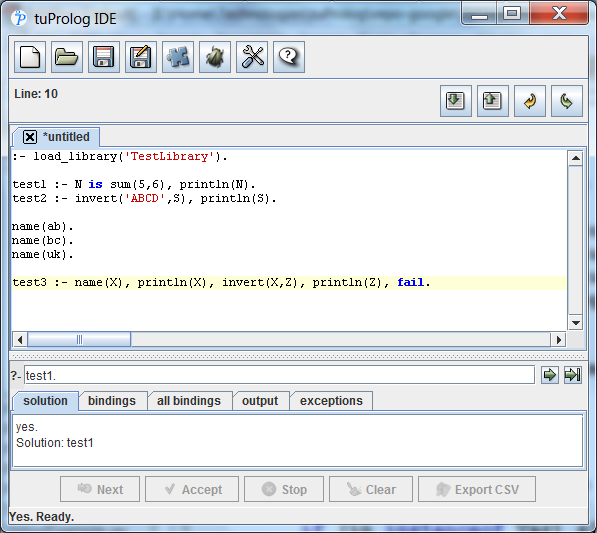
\includegraphics[width=10cm]{images/TestLibrary3}
  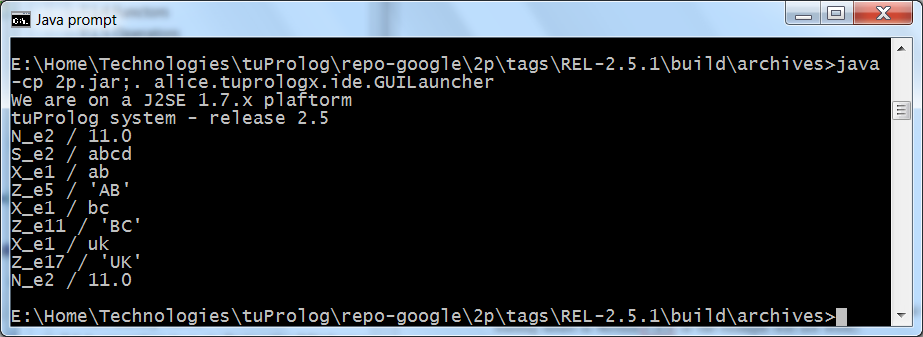
\includegraphics[width=12cm]{images/TestLibrary4}
  \caption{Loading a library from the Prolog side in the GUI \textit{(top)} and its output (\textit{bottom}). Be sure to read the loading issues in Section \ref{ssec:library-loading-issues}, or the example will not work.}
  \label{fig:testlibrary3}
\end{figure}
%
\begin{figure}
    \centering
  \includegraphics[width=9cm]{images/TestLibrary1}
  \includegraphics[width=9cm]{images/TestLibrary2}
  \caption{Loading a library from the Prolog side via the Library Manager icon in the \tuprolog{} GUI. The loading issues in Section \ref{ssec:library-loading-issues} still apply. Please note that the browse/save buttons in the dialog are \textit{not} to be used to load/save libraries, but only to load/save \textit{\tuprolog{} preferences} in the form of \texttt{.2p} files.}
  \label{fig:testlibrary1}
\end{figure}
%
\begin{figure}
    \centering
  \includegraphics[width=12cm]{images/TestLibrary5}
  \caption{Loading a library from the Prolog side on the CUIConsole: the output here is in the same terminal, as expected. Again, be sure to read the loading issues in Section \ref{ssec:library-loading-issues}, or the example will not work.}
  \label{fig:testlibrary5}
\end{figure}


\subsubsection{Naming issues}

\noindent When developing libraries, two naming issues may arise:
\begin{enumerate}
  \item the name of the predicate, functor or directive should contain a symbol that cannot legally appear in a Java method's name;
  \item a predicate and a directive with the same Prolog signature should be defined, but Java would not be able to distinguish method signatures differing for the return type only.
\end{enumerate}

\noindent To overcome these issues, a \textit{synonym map} must be set up, that maps the desired Prolog names onto legal Java method names, bypassing the standard naming convention.
%
This map must have the form of an array of \texttt{String} arrays, and be returned by the ad hoc \texttt{getSynonymMap} method (abstract in the base \texttt{Library} class).
%
For instance, an evaluable functor \texttt{+}, which cannot appear in a
Java method name, could be implemented by a defining a Java method with any name (say, \texttt{add}) and then map it onto the Prolog name by adding the array \texttt{\{"+", "add", "functor"\}} to the synonym map.

Libraries can also inherit from each other: a library can well extend a user library instead of the base \texttt{Library}, as in the case of the \texttt{HybridLibrary} discussed in the next Section.

%---------------------------------------------------------------
\subsection{Hybrid Java+Prolog libraries}
\label{ssec:hybrid-libraries}
%---------------------------------------------------------------

\begin{table}
    \begin{center}{\tt
    \begin{tabular}{p{12cm}}\hline
    \\
    public class HybridLibrary extends TestLibrary \{\\
    ~public String getTheory()\{\\
    ~~return "myprint(X) :- println(X).$\backslash$n" +\\
    ~~~~~~~~~"myprint(X) :- invert(X,Y), myprint(Y).$\backslash$n";\\
    ~\}\\
    \} \\
    \\
    \hline
    \\
    import alice.tuprolog.*;\\
    import alice.tuprolog.lib.*;\\
    \\
    public class HybridLibraryMain \{\\
    ~~public static void main(String[] args) throws Exception \{\\
	~~~~Prolog engine = new Prolog();\\
	~~~~Library lib2 = engine.loadLibrary("HybridLibrary");\\
	~~~~SolveInfo res = engine.solve("myprint(henry).");
	~~~~int count=0;
	~~~~while (engine.hasOpenAlternatives() \&\& count < 5)\{\\
	~~~~~~~~count++;\\
	~~~~~~~~res = engine.solveNext();\\
	~~~~\}\\
    \\
    \textrm{\textit{OUTPUT PRINTED:}}\\
    Lib2  LOADED\\
	X\_e1 / henry\\
	X\_e5 / yrneh\\
	X\_e9 / henry\\
	X\_e11 / yrneh\\
	X\_e13 / henry\\
	X\_e15 / yrneh\\
    \\\hline
    \end{tabular}
    }\end{center}
    \caption{A hybrid (mixed) Java + Prolog library \textit{(top)} and the corresponding test program \textit{(bottom)}. }
    \label{tab:HybridLibrary}
\end{table}

Since Java does not support non-determinism, a Java-only library is inherently
deterministic: however, non-determinism can be achieved via hybrid Java + Prolog
libraries, adding a %non-deterministic
Prolog layer on top of the %deterministic
Java layer.

To this end, a library can include a new piece of Prolog theory, embedded into the \texttt{getTheory} method.
%
This method returns a string\footnote{%
    In principle, only the external representation of this theory is constrained to the \texttt{String} form, the internal implementation being up to the developer; yet, using a Java \texttt{String} for wrapping the Prolog code guarantees self-containment while loading libraries through remote mechanisms such as RMI, and therefore constitutes the suggested form.
} (empty by default) containing the desired Prolog theory, and is automatically called when the library is loaded, so as to add the theory to the engine's configuration.

Table \ref{tab:HybridLibrary} shows a hybrid library where the theory in \texttt{getTheory} adds to \texttt{TestLibrary} the non-deterministic predicate \texttt{myprint/1}, whose (potentially infinite) solutions alternately print the argument in upper and lowercase.


%---------------------------------------------------------------
\subsection{Library loading issues}
\label{ssec:library-loading-issues}
%---------------------------------------------------------------

As shown in the above examples, a library can be loaded (and unloaded) dynamically into a running engine via Java, by means of the \texttt{loadLibrary} (\texttt{unloadLibrary}) methods; but it can also be loaded (unloaded) from Prolog, via the \texttt{load\_library/2} (\texttt{unload\_library/2} ) predicate.

However, caution is needed when using \texttt{2p.jar} to start the \tuprolog{} GUI (or the console-based CUI) if libraries are to be loaded from the Prolog side, because -- due to the behavior of the Java class loader -- a \textit{runnable} JAR cannot load classes that are not included in the JAR itself.
So, starting the \tuprolog{} GUI by double-clicking \texttt{2p.jar} (or by the equivalent \texttt{java -jar} command) will prevent libraries from being found and loaded from Prolog via the \texttt{load\_library/2} predicate or via the Library Manager in the GUI, except for the standard libraries packed into the \tuprolog{} JAR itself.

To bypass the problem, the JAR archive must \textit{not} be used as a \textit{runnable} JAR, but as a library JAR, specifying the main class explicitly:\\

\noindent \texttt{~java -cp MyLibrary.jar:2p.jar alice.tuprologx.ide.GUILauncher}\\

\noindent \texttt{~java -cp MyLibrary.jar:2p.jar alice.tuprologx.ide.CUIConsole}\\

\noindent In this way, the \texttt{-cp} option is taken into account by the class loader, making it possible to add a specific reference to the library to be loaded (e.g. \texttt{MyLibrary.jar} above).
On the contrary, running the JAR directly (via double click or via \texttt{java -jar}) causes the \texttt{-cp} option to be ignored in favor of the internal manifest properties, leading to a runtime failure.

In the future, the implementation will be improved using the URLClassLoader which can load classes from external JARs, so as to remove the limitation.


%---------------------------------------------------------------
\subsection{Library Name}
\label{ssec:library-name}
%---------------------------------------------------------------

The concept of library name is introduced in \tuprolog{} to separate the physical class name of a library from its logical name, both for clarity -- the library name can be shorter and more meaningful -- and to support multiple versions of the same library, enabling the dynamic upgrade of a library implementation.

By default, the library name is identical to the class name: however, a library can specify a different name by overriding the \texttt{getName} method.
%
Obviously, the full class name is always needed when loading the library, while the library name is used by \texttt{getLibrary} (and similar predicates) to return references to already-loaded libraries.

As an example, in Table \ref{tab:StringLibrary-NewStringLibrary} the \texttt{NewStringLibrary} class provides an alternate implementation of \texttt{StringLibrary}: this is why it \texttt{getName} is redefined so as to return \texttt{StringLibrary} as the \texttt{NewStringLibrary} library name.

\begin{table}
    \begin{center}{\tt
    \begin{tabular}{p{13.5cm}}\hline
    \\
    \mbox{~~~~}public class StringLibrary extends Library \{\\
    \mbox{~~~~~~~~}public boolean to\_lower\_case\_2(Term source, Term dest)\{\\
    \mbox{~~~~~~~~~~~~}String st = source.toString().toLowerCase();\\
    \mbox{~~~~~~~~~~~~}return unify(dest, new Struct(st));\\
    \mbox{~~~~~~~~}\}\\
    \mbox{~~~~~~}\ldots\\
    \mbox{~~~~~~}\textit{// the inherited getName returns "StringLibrary"}\\
    \mbox{~~~~~~}\ldots\\
    \mbox{~~~~}\}\\
    \\
    \hline
    \\
    \mbox{~~~~}public class NewStringLibrary extends Library \{\\
    \mbox{~~~~~~}public String getName()\{ return "StringLibrary"; \}\\
    \mbox{~~~~~~}\ldots\\
    \mbox{~~~~}\}\\
    \\
    \hline
    \end{tabular}
    }\end{center}
    \caption{Defining a new library with the same name as another.}
    \label{tab:StringLibrary-NewStringLibrary}
\end{table}


%-----------------------------------------------------------------------
\section{Augmenting Java via Prolog:\\the P@J framework}
\label{sec:p@j}
%-----------------------------------------------------------------------

The last dimensions of \tuprolog{}'s support to multi-paradigm, multi-language programming is still a form of \textit{augmenting} a language (that is, exploiting a language and a paradigm to increase the other)---in this case, augmenting Java from Prolog, exploiting the so-called \textit{P@J} framework \cite{short-patj-sac08}.

This approach makes it possible to ``inline intelligence'' into Java code, enabling Prolog to be used for implementing Java (abstract) methods, via Java reflection and suitable annotations.
%
The basic idea is that the methods to be implemented in Prolog are declared
\texttt{abstract} from the Java syntax viewpoint\footnote{%
  Of course, the corresponding class must be syntactically qualified \texttt{abstract}, too.
}, so that the Java compiler does not expect to find any implementation, while annotating them with the Prolog clauses that provide the actual implementations.
On the user side, the factory method \texttt{PJ.newInstance} will be used to automatically create a Java implementation of this method, which interacts with the Prolog engine in a totally transparent way.

The technique relies on advanced features of Java such generic types, wildcards, and type inference, as well as reflection to ``put things together''; for this reason, some syntax conventions are required for method signatures:
\begin{itemize}
  \item the Prolog predicate name must be identical to the Java method name;

  \item the argument types must be explicitly declared each with the corresponding bounding, and their names must start with \texttt{\$};

  \item the argument position in the Java method signature must reflect their role as input or output arguments in the Prolog predicate: the first are to be put in the argument list, and the latter in the return type.
\end{itemize}

\noindent The last requirement is necessary to bridge between the Prolog predicate syntax, where both input and output arguments are in the argument list (with nothing explicitly qualifying these roles, according to the declarative nature of the language), and the Java method syntax, where the only output argument is not in the argument list, but is ``returned from'' the method.

%---------------------------------------------
\subsection{Term taxonomy}
\label{ssec:p@j-term-taxonomy}
%---------------------------------------------

Here, too, a suitable taxonomy is needed to map the relevant Prolog types (term, atom, number, list, variable, etc) in Java; however, while the domain to represent is the same as above (Section \label{ssec:java-api-types}), the requirements due to type inference and strong type checking made it necessary to define one further, \textit{ad hoc} taxonomy as the base of the annotation layer.

The new hierarchy exploits the basic types in Figure \ref{fig:term-taxonomy} on page \pageref{fig:term-taxonomy} as its building bricks, and builds a new layer on top.
The new root is the abstract class \texttt{Term<X>}, whose definition exploits a recursive pattern to reify (represent) the type of the actual term content:

\begin{verbatim}
   abstract class Term<X extends Term<?>> {..}
\end{verbatim}

\noindent Accordingly, the term subclasses are defined as:

\begin{verbatim}
 class Atom extends Term<Atom> {..}
 class Int extends Term<Int> {..}
 class Double extends Term<Double> {..}
 class List<X extends Term<?>> extends Term<List<X>> {..}
 ...
\end{verbatim}

\noindent where, clearly, \texttt{Term<Int>} is used for a term containing an \texttt{Int}, \texttt{Term<Double>} for a term containing a \texttt{Double}, \texttt{Term<List<Int>>} for a term containing a \texttt{List<Int>}, etc.

Variables are a notable exception, because they must be able to contain values of the above types: for this reason, \texttt{Var<X>} is \textit{not} defined as a subtype of \texttt{Term<Var<X>>}, but directly of \texttt{Term<X>}.

\begin{verbatim}
 class Var<X extends Term<?>> extends Term<X> {..}
\end{verbatim}

\noindent As a consequence, both types \texttt{X} and \texttt{Var<X>} derive from the common ancestor Term<X>, which makes it possible to represent method arguments that may be a logical input or output---i.e., that must accept both a value (a term of type \texttt{X}) or a variable (a term of type \texttt{Var(X)}).

Thanks to this approach, a method definition like the following:

\begin{verbatim}
 boolean length(Term<? extends List<?>> list, Term<Int> size)
\end{verbatim}

\noindent can be read as follows:

\begin{itemize}
  \item list is a term containing any list, and size is an integer;

  \item both arguments can be either input or output.
\end{itemize}

\noindent The term hierarchy is completed by the \texttt{Compound} term family, which enables the definition of compound terms of any arity by means of a list-like approach---that is, starting from the empty compound term \texttt{Nil} and building bigger compounds with the \texttt{Cons} class constructor.
However, shortcut classes \texttt{Compound1}, \texttt{Compound2} and \texttt{Compound3} are provided for the user convenience to specify the most common terms of 1, 2 or 3 arguments:

\begin{verbatim}
 public abstract class Compound<X extends Compound<?>>
   extends Term<X> {..}

 public class Cons<H extends Term<?>, R extends Compound<?>>
   extends Compound<Cons<H,R>> implements Iterable<Term<?>>{..}

 public class Nil extends Compound<Nil> {..}

 public class Compound1<X1 extends Term<?>>
   extends Cons<X1,Nil> {..}

 public class Compound2<X1 extends Term<?>, X2 extends Term<?>>
   extends Cons<X1,Cons<X2,Nil>> {..}

 public class Compound3<X1 extends Term<?>, X2 extends Term<?>,
                        X3 extends Term<?>>
   extends Cons<X1,Cons<X2,Cons<X3,Nil>>> {..}
\end{verbatim}

%---------------------------------------------
\subsection{Examples}
\label{ssec:p@j-examples}
%---------------------------------------------

As an example, Table \ref{tab:pj-example1} shows a Java class \texttt{Perm} with the \texttt{permutation} method implemented in Prolog.
%
The Java method declaration specifies that there is one input argument and one output argument: the first (\texttt{\$X}) is a \texttt{List<Int>} (or a covariant type), the second (\texttt{\$Y}) is an \texttt{Iterable} over a \texttt{List<Int>} (or a covariant type).
The \texttt{Iterable} specification is needed to iterate over all solutions: if only the first solution is needed, \texttt{\$Y} could have been used instead of \texttt{Iterable<\$Y>}.

Moreover, since arguments are declared in the order (\texttt{\$X}), (\texttt{\$Y}) in the Java method signature, they will be mapped in this order on the Prolog predicate arguments: so (\texttt{\$X}) will map onto the first argument of \texttt{permutation/2}, and (\texttt{\$Y}) on the second argument.

In the client program, the \texttt{Perm} instance \texttt{p} is created indirectly via the \texttt{PJ.newInstance} factory method, whose argument is the corresponding \texttt{Class} meta-class, \texttt{Perm.class}.
Then, the \texttt{p} object can be used normally, like any other Java object: here it computes all the permutations of a given list of integers (built from an array, just to play with types), which is then iterated over by a \textit{for-each} loop that prints every result.
The actual type for both \texttt{\$X} and \texttt{\$Y}, \texttt{List<Int>}, is inferred automatically by the P@J runtime.

\begin{table}
{\footnotesize
\begin{tabular}[-1cm]{p{12cm}}
\begin{verbatim}
import alice.tuprologx.pj.annotations.*;
import alice.tuprologx.pj.engine.*;
import alice.tuprologx.pj.model.*;
import alice.tuprologx.pj.meta.*;
import java.util.List;
import java.util.ArrayList;
\end{verbatim}
\textsf{\emph{A Java class augmented via Prolog}}
\begin{verbatim}
abstract class Perm{
    @PrologMethod ( clauses = {
        "permutation([],[])." ,
        "permutation(U,[X|V]):-remove(U,X,Z),permutation(Z,V)." ,
        "remove([X|T],X,T)." ,
        "remove([X|U],E,[X|V]):-remove(U,E,V)."
        }
    )
    public abstract < $X extends List<Int>, $Y extends List<Int> >
                Iterable<$Y> permutation($X list);
}
\end{verbatim}
\textsf{\emph{A sample client class}}
\begin{verbatim}
public class PJexample {
  public static void main(String[] args) throws Exception {
    java.util.Collection<Integer> v = java.util.Arrays.asList(1,2,3);
    Perm p=PJ.newInstance(Perm.class);
    for (List<Int> list : p.permutation(new List<Int>(v))) {
        System.out.println(list.toJava());
    }
  }
}
\end{verbatim}
\textsf{\emph{Output printed:}}
\begin{verbatim}
    [1, 2, 3]
    [1, 3, 2]
    [2, 1, 3]
    [2, 3, 1]
    [3, 1, 2]
    [3, 2, 1]
\end{verbatim}
\end{tabular}
}\caption{A Java class exploiting Prolog for implementing an abstract method \textit{(top)} and a client using it \textit{(bottom)}. Note that the \texttt{Arrays.asList} method exploits the Java shortcut syntax for varargs.
To run the example, the \texttt{javassist.jar} library, used by the P@J runtime, must be in the class path: \texttt{E:>java~~-cp .;2p.jar;javassist.jar PJexample}
}
\label{tab:pj-example1}
\end{table}


\begin{table}
{\footnotesize
\begin{tabular}[-1cm]{p{12cm}}
\begin{verbatim}
import alice.tuprologx.pj.annotations.*;
import alice.tuprologx.pj.engine.*;
import alice.tuprologx.pj.model.*;
import alice.tuprologx.pj.meta.*;
\end{verbatim}
\textsf{\emph{Another Java class augmented via Prolog}}
\begin{verbatim}
@PrologClass(
	clauses = {"size(X,Y) :- length(X,Y)."}
)
public abstract class PJLength {	
    @PrologMethod abstract <$Ls extends List<?>, $Ln extends Int>
    Boolean size($Ls expr, $Ln rest);
    @PrologMethod abstract <$Ls extends List<?>, $Ln extends Int>
    $Ln size($Ls expr);
    @PrologMethod abstract <$Ls extends List<?>, $Ln extends Int>
    $Ls size($Ln expr);
    @PrologMethod abstract <$Ls extends List<?>, $Ln extends Int>
    Iterable<Compound2<$Ls,$Ln>> size();

    public static void main(String[] args) throws Exception {
        PJLength pjl = PJ.newInstance(PJLength.class);
        java.util.List<?> v = java.util.Arrays.asList(12,"ok",false);
        List<?> list = new List<Term<?>>(v);
        Boolean b = pjl.size(list, 3);   // true
        Int i = pjl.size(list);          // length is 3
        List<?> l = pjl.size(3);         // produces [_,_,_]
        int cont = 0;
        for (Term<?> t : pjl.size()) {   // [],[_],...,[_,_,_,_,_]
            System.out.println(t);
            if (cont++ == 5) break;
        }
    }
}\end{verbatim}
\textsf{\emph{Output printed:}}
\begin{verbatim}
    Compound:'size'(List[],Int(0))
    Compound:'size'(List[Var(_)],Int(1))
    Compound:'size'(List[Var(_), Var(_)],Int(2))
    Compound:'size'(List[Var(_), Var(_), Var(_)],Int(3))
    Compound:'size'(List[Var(_), Var(_), Var(_), Var(_)],Int(4))
    Compound:'size'(List[Var(_), Var(_), Var(_), Var(_), Var(_)],Int(5))
\end{verbatim}
\end{tabular}
}\caption{Another Java class exploiting Prolog for method implementation. The \texttt{length/2} predicate used in the \texttt{clauses} section on top is part of the standard ISO list management predicates.}
\label{tab:pj-example2}
\end{table}

\begin{table}
{\footnotesize
\begin{tabular}[-1cm]{p{12cm}}
\begin{verbatim}
import alice.tuprologx.pj.annotations.*;
import alice.tuprologx.pj.engine.*;
import alice.tuprologx.pj.model.*;
import alice.tuprologx.pj.meta.*;
\end{verbatim}
\textsf{\emph{Another Java class augmented via Prolog}}
\begin{verbatim}
@PrologClass (
  clauses={"arc(a,b)." , "arc(a,d)." , "arc(b,e)." , "arc(d,g).",
           "arc(g,h)." , "arc(e,f)." , "arc(f,i)." , "arc(e,h)."}
)
public abstract class PJPath {
  @PrologMethod (
    clauses = {	"path(X,X,[X]).",
                "path(X,Y,[X|Q]):-arc(X,Z),path(Z,Y,Q)."}
  )
  public abstract <$X,$Y,$P> Iterable<$P> path($X from, $Y to);

  public static void main(String[] s) throws Exception {
    PJPath pjp = PJ.newInstance(PJPath.class);
    for (Object solution : pjp.path(new Atom("a"), new Var<Atom>("X"))) {
      System.out.println(solution);
    }
  }
}\end{verbatim}
\textsf{\emph{Output printed:}}
\begin{verbatim}
  List[Atom(a)]
  List[Atom(a), Atom(b)]
  List[Atom(a), Atom(b), Atom(e)]
  List[Atom(a), Atom(b), Atom(e), Atom(f)]
  List[Atom(a), Atom(b), Atom(e), Atom(f), Atom(i)]
  List[Atom(a), Atom(b), Atom(e), Atom(h)]
  List[Atom(a), Atom(d)]
  List[Atom(a), Atom(d), Atom(g)]
  List[Atom(a), Atom(d), Atom(g), Atom(h)]
\end{verbatim}
\end{tabular}
}\caption{Another Java class exploiting Prolog for method implementation.}
\label{tab:pj-example3}
\end{table}


Two further examples are shown in Table \ref{tab:pj-example2} and Table \ref{tab:pj-example3}, respectively.
The first operates on lists, and finally generates (and prints) five ``lists of anything'' of 1,2,3,4,5 arguments; the second computes the path between two given nodes in a graph. In both cases, Prolog is delegated the reasoning part, while Java is exploited as the front-end to the user.
Technically, attention is required to distinguish Java lists (i.e., instances of \texttt{java.util.List} and its subclasses) from P@J \texttt{List}, which handles terms like \texttt{Term<X>}; moreover, the example in Table \label{tab:pj-example2} shows the inner structure of compounds.

For completeness, Table Table \ref{tab:pj-example4} shows a last, more complex example, where the Prolog code specifies a parser for arithmetic expressions.

\begin{table}
{\footnotesize
\begin{tabular}[-1cm]{p{12cm}}
\begin{verbatim}
import alice.tuprologx.pj.annotations.*;
import alice.tuprologx.pj.engine.*;
import alice.tuprologx.pj.model.*;
import alice.tuprologx.pj.meta.*;

@PrologClass
public abstract class PJParser {
  @PrologMethod (clauses={"expr(L,R):-term(L,R).",
                          "expr(L,R):-term(L,['+'|R2]), expr(R2,R).",
                          "expr(L,R):-term(L,['-'|R2]), expr(R2,R)."})
  public abstract <$E extends List<?>, $R extends List<?>>
  Boolean expr($E expr, $R rest);

  @PrologMethod (clauses={"term(L,R):-fact(L,R).",
                          "term(L,R):-fact(L,['*'|R2]), term(R2,R).",
                          "term(L,R):-fact(L,['/'|R2]), term(R2,R)."})
  public abstract <$T extends List<?>, $R extends List<?>>
  Boolean term($T term, $R rest);
	
  @PrologMethod (clauses={"fact(L,R):-num(L,R).",
                          "fact(['(' | E],R):-expr(E,[')'|R])."})
  public abstract <$F extends List<?>, $R extends List<?>>
  Boolean fact($F fact, $R rest);
	
  @PrologMethod (clauses={"num([L|R],R):-num_atom(_,L)."})
  public abstract <$N extends List<?>, $R extends List<?>>
  Boolean num($N num, $R rest);
	
  public static void main(String[] args) throws Exception {
    PJParser ep = PJ.newInstance(PJParser.class);
    String tokenizer_regexp =
      "(?<!^)(\\b|(?=\\()|(?=\\))|(?=\\-)|(?=\\+)|(?=\\/)|(?=\\*))";
    List<Atom> exp1 = new Atom("12+(3-4)").split(tokenizer_regexp);
    List<Atom> exp2 = new Atom("(12+(3-4))").split(tokenizer_regexp);
    System.out.println(ep.expr(exp1, List.NIL)); // 12+(3*4)   expression ?
    System.out.println(ep.fact(exp1, List.NIL)); // 12+(3*4)   factor ?
    System.out.println(ep.expr(exp2, List.NIL)); // (12+(3*4)) expression ?
    System.out.println(ep.fact(exp2, List.NIL)); // (12+(3*4)) factor ?
  }
}\end{verbatim}
\end{tabular}
}\caption{A parser for arithmetic expressions encoded in Prolog inside an annotated Java program. The output prints \texttt{true}, \texttt{false}, \texttt{true}, \texttt{true} in this order, since 12+(3*4) is an expression but not a factor, while (12+(3*4)) is both an expression and a factor.}
\label{tab:pj-example4}
\end{table}

%******************************************************************************%
%=======================================================================
\chapter[Multi-paradigm programming in Prolog and .NET]{Multi-paradigm program-\\ming in Prolog and .NET}
\label{ch:mpp-in-dotnet}
%=======================================================================

\tuprolog{}.NET now provides the user with the same features as the Java version, extending and specializing the multi-paradigm, multi-language experience to the plethora of languages available onto the Microsoft .NET platform.
In this Chapter, the impact of such change is discussed, both in terms of specific conceptual concepts (namely, \textit{language conventions} to handle multiple languages) and new/specialized libraries and predicates to be used for language interaction.

Since the current status of \tuprolog{}.NET depends \textit{a)} on its past history and \textit{b)} on the IKVM tool \cite{ikvm}, the two following Sections summarize its evolution from version 2.1 and the basics of IKVM translation, respectively.

While their reading is recommended to everyone, the reader wishing only to exploit \tuprolog{}.NET in its current version can safely bypass them and jump directly to Section \ref{sec:dotnet-tuprolog-now}.

%-----------------------------------------------------------------------
\section{A bit of history}
\label{sec:dotnet-tuprolog-history}
%-----------------------------------------------------------------------

%--------------------------------------------
\subsection{\tuprolog{} 2.1 and CSharpLibrary}
\label{ssec:dotnet-tuprolog2.1}
%--------------------------------------------

\tuprolog{}.NET appeared as a usable tool for the first time in April 2007, with the .NET conversion of \tuprolog{} 2.1; an earlier, experimental version had been made with version 2.0, but was never officially published.

tuProlog.NET 2.1 run on Microsoft .NET 2.0 and on Mono 1.2.5\footnote{The MONO version required a source tuning for the \texttt{TheoryManager.find} method.}, and was a complete rewriting in C\# of the original Java code: the executable became a .NET \texttt{exe} file, and all the libraries became .NET \texttt{dll} assemblies.

The Java-based, key feature to multi-paradigm-programming, \textit{JavaLibrary}, was replaced by a corresponding \textit{CSharpLibrary}, which provided the very same features, except for a few syntactic changes:
\begin{itemize}
  \item any \texttt{java\_\textit{xxx}} predicate was renamed as \texttt{csharp\_\textit{xxx}}.

  \item C\# objects defined in other namespaces than \texttt{System} required that the new namespace be explicitly passed to the predicate creating the object: so, \texttt{java\_object/3} became \texttt{csharp\_object/4}:\\
        \texttt{csharp\_object(\textit{\textbf{AssemblyName}}, \textit{ClassName}, \textit{ArgumentList}, \textit{ObjRef})}\\
      Moreover, the assembly containing the definition of the object type must be in the same folder as the \texttt{alice-tuProlog.dll} file.

\item an \textit{ad hoc} predicate was added for array creation, instead of using the standard \texttt{csharp\_object/3}-\texttt{/4} resulting from the direct conversion of JavaLibrary predicates:
    \texttt{csharp\_array(\textit{AssemblyName}, \textit{Type}, \textit{Length}, \textit{ObjRef})}
\end{itemize}

An annoying limitation concerned the loading of user-defined libraries (and theories), which had to be in the same folder as the \tuprolog{} (\texttt{IDE.exe} or \texttt{CUIConsole.exe}) executable.

From the developers' viewpoint, using \tuprolog{} classes in a Visual Studio project required a reference to the \texttt{alice-tuProlog.dll} assembly be added to the project, and the \texttt{tuProlog} namespace be imported in the usual C\# fashion (e.g. \texttt{using tuProlog;}).

%--------------------------------------------
\subsection{\tuprolog{} 2.1.3: CSharpLibrary + exceptions}
\label{ssec:dotnet-tuprolog2.1.3}
%--------------------------------------------

As a further step towards the convergence of the .NET and Java versions, the ``\tuprolog{} 3'' project --later renamed as 2.1.3 -- was started to add the exceptions support, being developed for the Java version, to the .NET version, too.
However, this version was never officially released, because of the quasi-simultaneous
development of \tuprolog{} 2.2, whose \textit{CLILibrary} could provide a much larger interest from the multi-paradigm, multi-language viewpoint.

%--------------------------------------------
\subsection{\tuprolog{} 2.2 and CLILibrary}
\label{ssec:dotnet-tuprolog2.2}
%--------------------------------------------

Version 2.2\footnote{%
    Unfortunately, version numbering for .NET was incoherent with the Java version at that time: in Java, 2.2 was the version that introduced the exception support, which was absent in 2.2 for .NET because the development \tuprolog{} 2.1.3, where exceptions were being added, occurred quasi-simultaneously, but not in time for the two projects to converge. In addition, this version was never tested on Mono.
} was a milestone in \tuprolog{}.NET history, as it generalized \textit{CSharpLibrary} to enable multi-language programming with \textit{virtually any language available on the .NET platform}, rather than C\# only (unfortunately, it lacked exception support, due to the race between the two quasi-simultaneous projects).

To this end, the concept of \textit{Language Convention} was introduced to encapsulate the language-specific aspects, so that a single library -- renamed \textit{CLILibrary} instead of \textit{CSharpLibrary} -- could handle any language.
%
Each convention contains the syntax conversion operations and the post-compilation transformations required for a given language.
Conventions were developed for C\#, J\#, VisualBasic.NET, F\#, Eiffel.NET and
IronPythonStudio.

Following the generalization renaming of \textit{CSharpLibrary} as \textit{CLILibrary}, a few syntactic changes were also made:
\begin{itemize}
  \item any \texttt{csharp\_\textit{xxx}} predicate of CSharpLibrary was renamed here as \texttt{cli\_\textit{xxx}}; this applies both to predicates derived from the JavaLibrary (of the form \texttt{java\_\textit{xxx}}) and to predicates added by CSharpLibrary, like \texttt{csharp\_array/4};

 \item to create objects bound to a particular \textit{Convention}, the \texttt{cli\_object/5} predicate was introduced whose first argument specifies the convention to be used:\\
     \texttt{cli\_object(\textit{\textbf{Convention}}, \textit{AssemblyName}, \textit{ClassName},\\
     \mbox{~~~~~~~~~~~}\textit{ArgumentList}, \textit{ObjRef})}

 \item furthermore, for those .NET programming languages whose constructor function is not constrained to coincide with the class name, and therefore require such a name to be explicitly specified on object creation, the \texttt{cli\_object/6} predicate was introduced:\\
     \texttt{cli\_object(\textit{Convention}, \textit{AssemblyName}, \textit{ClassName},\\
     \mbox{~~~~~~~~~~~}\textbf{\textit{ContructorName}}, \textit{ArgumentList}, \textit{ObjRef})}

 \item two convention handling predicates, also usable as directives, were introduces to load/unload conventions to/from a Prolog theory:\\
     \texttt{load\_convention(\textit{Assembly}, \textit{ConventionName}, \textit{ConventionAtom})}\\
     \texttt{unload\_convention(\textit{ConventionAtom})}.
\end{itemize}

From the developers' viewpoint, the new aspect is how to define new conventions: this is done by starting a new project (class library), importing the \texttt{alice-tuprolog.dll} reference and implement a new class extending \texttt{tuProlog.Convention} in the \texttt{tuProlog.Conventions} namespace.

The \texttt{dll} generated by the compilation must then be moved to the main project compiling folder.


%--------------------------------------------
\section{IKVM Basics}
\label{sec:dotnet-ikvm}
%--------------------------------------------

IKVM.NET \cite{ikvm} is basically a .NET implementation of Java (language, infrastructure, tools) enriched with special tools for Java/.NET conversion.
Its distribution, which adheres to the \textit{zlib} open source license, includes:
\begin{itemize}
  \item a .NET implementation of a Java Virtual Machine;
  \item a Java class library, based on OpenJDK, re-implemented in .NET;
  \item tools for Java/.NET inter-operability---in particular, the \texttt{ikvmc} bytecode translator that converts Java bytecode to Microsoft .NET Common Intermediate Language (CIL).
\end{itemize}

\noindent Both Microsoft .NET 2.0 and Mono platforms 2.0 are supported, both for \textit{x86} and \textit{x64} architectures. If necessary, the source pack is also available.

Debugging is also very well supported: if the Java sources are available, proper information can be generated\footnote{The option must be specified to generate the \texttt{pdb} (\textit{Program Debug Database}) file, to be copied to the application folder in Visual Studio.} that enable Microsoft Visual Studio to keep the .NET and and Java sources in sync, following the program execution on the Java source, too, as well as enabling breakpoints, variable inspection, etc.

%--------------------------------------
\subsection{Dynamic vs. Static modality}
\label{ssec:ikvm-dynamic-static}
%--------------------------------------

IKVM can work in two modalities. In the \textit{dynamic} modality, Java applications are converted in .NET on-the-fly and immediately executed; in the \textit{static} modality, instead, Java applications (or libraries) are translated into a .NET assembly, to be used to develop a .NET native application.

The dynamic modality is supported by the \texttt{ikvm} tool, which is analogous to Java's \texttt{java} interpreter\footnote{Most command line options work identically with both tools.}: so, a Java application can be executed in .NET as in would be in a Java-enabled machine, just replacing \texttt{java} with \texttt{ikvm}, in a totally user-transparent way.
Quite notably, the class loading mechanisms in this modality behaves exactly as in Java, with the same class path options.
The only drawback is performance, which is obviously penalized by the on-the-fly translation.

The static modality is supported by the \texttt{ikvmc} tool, which generates a \texttt{dll} or \texttt{exe} .NET assembly (depending whether the translation concerns a Java library or application, respectively) converting Java types to .NET types.
Obviously, this tool has no Java counterpart: its options control the target architecture (\textit{x86} or \textit{x64}), the kind of output (\texttt{dll}/\texttt{exe}), etc.
Unlike the previous case, here the Java class loading mechanisms has some limitations, that are discussed below.
One possible drawback is IKVM choice of translating the Java \textit{package} visibility into .NET \textit{internal}'s, making it impossible to access such properties and methods from other assemblies (even though they were accessible in the Java architecture).

%--------------------------------------
\subsection{Class loading issues}
\label{ssec:ikvm-class-loading}
%--------------------------------------

The class loading mechanism is perhaps the major issue when translating Java applications to .NET, because of the very different approach adopted by the two architectures, which makes it difficult to define a general mapping. In fact,
\begin{itemize}
  \item the Java approach is based on the \textit{class path} concept, which defines the set of paths where classes must be looked for;
  \item the .NET approach, instead, exploits the current folder, the Global Assembly Cache (GAC) and configuration files for the same purpose.
\end{itemize}

\noindent In order to bridge this gap, IKVM adopts the following intelligent approach:
\begin{itemize}
  \item each \textit{statically-generated} assembly is associated to its own class loader---either a user-supplied one, or the default one;

  \item the default class loader looks for classes:
  \begin{enumerate}
    \item first, in the assembly itself;
    \item then, in all the assemblies \textit{directly referenced} by the former.
  \end{enumerate}
\end{itemize}

\noindent This approach guarantees that classes are always found \textit{if all dependencies are statically expressed}, i.e. if all the libraries used by an application are statically known, and their references are added in the application project.
Problems are to be expected, instead, for dynamically loaded classes, whose references were not included in the project---and whose assemblies, therefore, are not considered by the class loader.

To overcome this issue, four alternatives can be followed:
\begin{enumerate}
  \item creating a \textit{single assembly}, if size is not a problem and run-time modularity is irrelevant (that is, loading all modules even when just one is actually used is irrelevant);
  \item adding a static reference (\texttt{-r} option) to the library to be dynamically loaded, when the application is translated to .NET: then, the default .NET loading will locate the library, but the need to specify all its details (including version number) cancels most of the advantage of dynamic loading, since any change in the library to be loaded still requires a rebuild;
  \item using the special \texttt{ikvm.runtime.AppDomainAssemblyClassLoader}
  class loader provided by IKVM;
  \item writing an ad-hoc class loader, typically extending \texttt{URLClassLoader}: this is perhaps the most flexible, but also the user-heaviest, solution.
\end{enumerate}

\noindent One further interesting aspect is that the IKVM implementation of Java's \texttt{Class.forName} method adopts a more general behavior than Java's default implementation, supporting the dynamic loading of classes also \textit{beyond} the current assembly even without special options, provided that their \texttt{AssemblyQualifiedName} is specified; otherwise, only the current assembly is checked.

So, a Java application that exploited \texttt{Class.forName} for dynamic class loading, that could originally load only classes in the application JAR unless properly launched (see Section \ref{ssec:library-loading-issues}), will be able to load .NET\footnote{The reason why this feature is limited to .NET classes is, trivially, that only .NET classes possess the \texttt{AssemblyQualifiedName} property and the other assembly details (version, culture, public key token).} classes beyond the application's own assembly when translated to .NET via IKVM.

%--------------------------------------
\subsection{The other way: writing .NET applications in Java}
\label{ssec:ikvm-writing-app-in-java}
%--------------------------------------

Beyond converting Java applications in .NET, IKVM also supports the opposite direction---that is, writing .NET applications \textit{in Java}, as if this were one of .NET-supported languages.

This feature is provided by the \texttt{ikvmstub} tool, which generates a Java JAR archive from a .NET assembly (\texttt{dll}/\texttt{exe}).
As the tool name suggests, the generated JAR is just a stub, containing all the Java classes and interfaces corresponding to the .NET originals, but no actual implementation, since this will be written directly in Java: its purpose is just to satisfy the \texttt{javac} compiler's type checking, and enable the code completion feature on the IDE (e.g. Eclipse) used for the Java application development.

In this way, a Java application can be written (in Java---using Eclipse, Netbeans, etc.)) that exploits the .NET types extracted from the .NET original assemblies.
This application can be compiled with \texttt{javac} as usual, specifying the above stub JAR in the class path (\texttt{-cp} option).

Obviously, such an application can \textit{not} be run in Java with the standard \texttt{java} interpreter, as the above stub JAR does not contain any actual implementation---nor would that be reasonable, since the goal was to exploit Java to write a .NET application, not a Java one.
%
Instead, the resulting ``fake'' Java application is to be translated via \texttt{ikvmc}, and then executed \textit{in .NET} where the original assemblies provide the ``missing'' classes.

\medskip

In this context, .NET concepts are mapped onto suitable Java concepts by \texttt{ikvmstub} as follows:
\begin{itemize}
  \item \textit{namespaces} are mapped onto Java packages, pre-pending the \texttt{cli.} prefix to prevent name clashes;
  \item \textit{properties} are mapped onto a pair of Java \texttt{\textit{get}}/\texttt{\textit{set}} methods;
  \item \textit{enumerations} are mapped onto classes extending \texttt{cli.System.Enum}, with static fields with integer values for each possible value of the .NET enumerative type;
      % MAYBE IN THE FUTURE THIS WILL CHANGE, AND ENUM WILL BE USED.
  \item \textit{delegates} are mapped onto a Java class and a nested helper \texttt{Method} interface: the class derives from \texttt{System.MulticasDelegate} and has the same name as the original delegate, while the nested interface always declares an \texttt{Invoke} method whose signature matches the delegate: this method is called when an event occurs. This is why, the class constructor takes as its argument an object implementing the \texttt{Method} interface, whose implementation of \texttt{Invoke} does the actual job.
  \item \textit{events} are mapped onto a pair of Java \texttt{\textit{add\_*}}/\texttt{\textit{remove\_*}} methods, whose argument is an object of the class representing the delegate;
  \item \textit{params} is mapped onto an array of \texttt{Object}s;
          % MAYBE IN THE FUTURE THIS WILL CHANGE, AND GENERICS WILL BE USED.
  \item \textit{attributes} are mapped onto a Java class with the same name as the .NET attribute, plus a pair of Java \texttt{\textit{get}}/\texttt{\textit{set}} methods for each property defined by the attribute.\footnote{The java class also includes a nested Java annotation, called \texttt{Annotation}, which defines Java methods homonomous to the .NET attribute properties: any reference to such an annotation in the Java code will be translated into the corresponding .NET attribute when the application is converted to .NET. However, only read properties are supported, even if the original .NET attribute properties were read/write.}
\end{itemize}

%-----------------------------------------------------------------------
\section{\tuprolog.NET now}
\label{sec:dotnet-tuprolog-now}
%-----------------------------------------------------------------------

The management difficulties in keeping coherent two such evolving projects (the Java and the .NET versions) indicated that the approach of a separate development was not sustainable in the perspective.
This led to a complete strategic change, resulted into the adoption of the IKVM \cite{ikvm} bytecode translator as a tool to automate the generation of \tuprolog.NET \textit{from the same Java bytecode} (other than sources) as the Java version, which could then become the only one to be actively maintained ``by hand''.

Despite some (minor) performance issues (the IKVM-generated \tuprolog{} version appears 15\% slower, in the average, than its Java counterpart), the approach turned out to be winning, enabling the two platforms to converge for all they have in common---namely, everything other than the \textit{CLILibrary} and the .NET-specific issues.

%--------------------------------------------
\subsection{Highlights}
\label{ssec:dotnet-highligths}
%--------------------------------------------

\tuprolog{}.NET 2.5 builds on top of the winning idea of version 2.2 (language conventions for multi-language interoperability with Prolog), but goes farther by exploiting the value-added brought by the IKVM approach: the chance to use \textit{even Java} as if it were directly available on the .NET platform.
%
This extra value spreads into several directions:
\begin{itemize}
  \item .NET objects can be accessed, in addition to Java objects, via       \textit{OOLibrary} -- the renovated version of JavaLibrary -- from \tuprolog{};

  \item .NET applications can be developed (instead of Java applications, which obviously require the \tuprolog{} Java version) that exploit \tuprolog{} as a third-party library, with the only difference that a \texttt{dll} assembly is to be referenced by the (Visual Studio) project, instead of a JAR archive;

  \item the whole P@J framework for implementing Java methods in Prolog remains available, and takes a newer form in the .NET context;

  \item \tuprolog{} libraries can be written in Java, as well as in other .NET languages, resulting into a \texttt{dll} assembly in the end;

  \item Java can be used together with C\#, F\#, and other .NET languages in the same .NET application, where \tuprolog{} can possibly play the role of the director (orchestrator, coordinator) in-front-of or behind the scenes.
\end{itemize}

\noindent In the next Sections of this Chapter, these dimensions are discussed and explored, roughly following the same structure as Chapter \ref{ch:mpp-in-java}.

\begin{table}
{\small
\begin{tabular}{|p{2cm}|p{2cm}|p{2.4cm}|p{2cm}|p{2.2cm}|}
\hline
  Benchmark & Java direct & Java via Prolog & C\# direct & C\# via Prolog\\
  Math   & 118 & 182 & 116 & 118\\
  Concat & 185 & 211 & 162 & 161\\
  Sort   & 147 & 149 & 142 & 143\\
  \hline
\end{tabular}}
  \caption{Performance comparison between Java and C\# code executed directly or via \tuprolog{}.NET (times in milliseconds).}\label{tab:dotnet-benchmarks}
\end{table}

From the performance viewpoint, the experience of the older \tuprolog{}.NET 2.2 (see Section \ref{ssec:dotnet-tuprolog2.2}) showed that an overhead is to be expected on Java applications.
To quantify it in some common situations, Table \ref{tab:dotnet-benchmarks} shows the average execution times of three micro-benchmarks (\textit{math}, \textit{concat} and \textit{sort}) when written in Java and C\#, executed directly and via \tuprolog{}.NET, respectively: \textit{math} performs algebraic operations on real numbers, \textit{concat} concatenates strings via the \texttt{StringBuilder} class available in both languages, and \textit{sort} sorts an array of integer numbers via quicksort.

Quite clearly, the execution of Java code via IKVM introduces an overhead\footnote{These figures are not very sensitive to the time overhead of class loading, because the classes to be loaded here are few and small: however, the first iterations of the test program do show higher execution times for this reason.} whose weight depends of the specific operation area, and whose cause is mainly the IKVM implementation of Java libraries: in fact, the \textit{sort} test, where IKVM incorporates its own implementation of the Java library instead of using the default one, is not affected in its performance.

Conversely, the execution of .NET code (the implementation language selected is irrelevant for this comparison) is basically overhead-free even when triggered from \tuprolog{}.

%-----------------------------------------------------------------------
\section{Using .NET from Prolog: OOLibrary}
\label{sec:dotnet-oolibrary}
%-----------------------------------------------------------------------

\subsubsection{Motivation}

Since \tuprolog{}.NET is automatically generated from the Java sources via IKVM, JavaLibrary is also available for free; however, since this library was designed for Java, it inherently supports Java concepts and constructs, but is obviously unaware of the features that are specific to .NET languages, such as properties, delegates, etc.
%
So, while .NET objects could be loaded and exploited via JavaLibrary ``as is'' (thanks to the extended semantics of \texttt{Class.forName} discussed in Section \ref{ssec:ikvm-class-loading}), their support would be imperfect, for three main reasons:
\begin{itemize}
  \item the lack of support for some .NET language constructs;
  \item the different Java naming convention for methods w.r.t. Java;
  \item the code reorganisation performed behind-the-scenes by the .NET compilers, which sometimes change the names of syntactic elements---for instance, properties are compiled by adding a pair of getter/setter methods.
\end{itemize}

\noindent These aspects are put well in evidence by the example below, which refers to a class \texttt{Student} (written in C\#) defining a ``standard'' student with some ``obvious'' properties:

\begin{verbatim}
    java_object('CStudent.Student, CStudent',
                [123456,'John','Smith'], Obj),
    Obj <- 'PrintStudent' returns Value,
    Obj <- 'get_Name' returns Value,
    Obj <- 'set_Name'('Albert').
\end{verbatim}

\noindent As the first line shows, a \texttt{Student} instance can be created via \texttt{java\_object/3} \textit{as if it were a Java class}, but only by means of its \texttt{\textit{AssemblyQualifiedName}}---possibly specifying also its version, culture and public key.
Moreover, the method name must be quoted, since the .NET conventions require the first letter to be capitalized.
Last but not least, access to properties -- that the translated JavaLibrary does not know  as such -- must be mediated by the get/set methods added by the .NET compiler, with a loss both of expressiveness (the \texttt{Obj.Property} notation is lost) and of transparency (the compiler transformations must be known to bypass the problem).

This is why the direct use of JavaLibrary is \textit{deprecated} in \tuprolog{}.NET, which provides a better alternative: \textit{OOLibrary}.

OOLibrary extends JavaLibrary by enabling \tuprolog{}.NET to interact with both Java and .NET software components. In principle, any .NET language can be supported, although the current distribution includes the support only for the most widely used .NET languages (C\#, F\# and VB.NET), other than Java itself; however, the support for other .NET languages can be easily added, by defining further \textit{language conventions}.

\subsubsection{Language Conventions}

Language conventions are \tuprolog{} means to separate and embed the language-specific aspects from the library core: originally introduced in \tuprolog{}.NET 2.2 (see Section \ref{ssec:dotnet-tuprolog2.2} above), they work as a bridge between the language-specific naming issues and the underlying Java-based machinery.

Conventions define standard methods (Table \ref{tab:dotnet-convention-interface}) that express how the name of the required entity (class, method, property, public field, etc) must be modified to take into account the compiler modifications, so that the original .NET name may be transparently used in a \tuprolog{} program.
%
\begin{table}
{\small
\begin{verbatim}
public abstract class Convention{
  public abstract string Name ...
  public virtual string GetNamespace(string oldNamespace) ...
  public virtual string GetClassName(string oldClassName) ...
  public virtual string GetMemberName(string oldMemberName) ...
  public virtual string GetFieldName(string oldFieldName) ...
  public virtual string GetPropertyGetterName(string oldPropName) ...
  public virtual string GetPropertySetterName(string oldPropName) ...
  public virtual bool IsArrayClass(string className)...
  public static Convention LoadConvention(string assembly,
                                          string className)...
}
\end{verbatim}
}
\caption{The public interface of the root \texttt{Convention} class. Any actual convention for a given language must specialize from this class according to the language details.}
\label{tab:dotnet-convention-interface}
\end{table}
%
Obviously, the \texttt{GetXX} methods convert the name of the corresponding entity, while \texttt{IsArrayClass} checks whether the class represents an array---typically verifying if its name ends with \texttt{"[]"}, but this behavior can be redefined if a language adopts a different naming scheme.
The abstract \texttt{Name} property represents the name of the convention: each actual convention will set it to the corresponding language (i.e., \texttt{"csharp"}, \texttt{"fsharp"}, etc.)

Currently, four conventions are included in the distribution:
\begin{itemize}
  \item \textbf{C\#}: in this language all the names, except for field names, must start with a capital letter: so the \texttt{GetXX} methods must change the letter case accordingly. Moreover, since properties are compiled in a pair of \texttt{get\_}/\texttt{set\_} methods, the two \texttt{GetPropertyGetterMethod} and \texttt{GetPropertySetterMethod} methods return strings like \texttt{get\_\textit{PropName}} / \texttt{set\_\textit{PropName}}, respectively.

  \item \textbf{F\#}: this convention is identical to C\#'s.

  \item \textbf{VB.NET}: this convention is identical to C\#'s, except for arrays, that are defined through \texttt{()} in Visual Basic .NET instead of \texttt{[]}: so, the \texttt{IsArrayClass} method is redefined accordingly.

  \item \textbf{Java} this convention operates opposite to the above, changing method and field names so that they start with a lowercase letter; class names are checked for starting with an uppercase letter, and packages are changed to all-lowercase.
\end{itemize}

\noindent Since conventions and OOLibrary are part of \tuprolog{}.NET only, they are both implemented in C\#, to avoid unnecessary intermediate conversions.

\subsubsection{OOLibrary: predicates}

OOLibrary puts together the easy of use and immediateness of JavaLibrary with the convention-based inspiration of the former \textit{CLILibrary} (found in version 2.2): Table \ref{tab:dotnet-oolibrary-interface} lists its predicates.
%
\begin{table}
{\small
\begin{verbatim}
public class OOLibrary {
  public bool new_object_4(Term conventionName, Term className,
                           Term args, Term objRef)
  public bool destroy_object_1(Term objRef)
  public bool method_call_3(Term objRef, Term methodName, Term resRef)
  public bool load_convention_3(Term assemblyName,
                                Term conventionName, Term convRef)
  public bool dload_convention_3(Term assemblyName,
                                Term conventionName, Term convRef)
  public bool unload_convention_1(Term convRef)
}
\end{verbatim}
}\caption{The public interface of the \texttt{OOLibrary} class. In addition, the \texttt{$<-$/2}, (\texttt{$<-$},\texttt{returns})\texttt{/3} and \texttt{.} operators are defined for method calling and field/property access with the \texttt{get}/\texttt{set} pseudo-methods, exactly as in JavaLibrary.}
\label{tab:dotnet-oolibrary-interface}
\end{table}

\noindent These methods modify the names of the received entities according to the specified convention, then call the corresponding JavaLibrary methods.
For instance, if the target object is written in C\#, OOLibrary:
\begin{itemize}
  \item retrieves the associated convention (if any);
  \item changes the method name accordingly;
  \item invokes \texttt{java\_call\_3} to perform the operation.
\end{itemize}

\noindent The \texttt{dload\_convention\_3} method is the directive version of \texttt{load\_convention\_3}), the difference being in the lifetime of the loaded convention: the directive loads a convention for the whole life of the current \tuprolog{} engine, while the standard version loads it for the duration of the current query only.

%-------------------------------------
\subsection{Examples}
\label{sec:dotnet-oolibrary-examples}
%-------------------------------------

%To show OOLibrary at work, it is first necessary to start \tuprolog{}.NET and \textit{manually remove JavaLibrary} (loaded by default as a side effect of the translation from Java) via the Library Manager, and then and \textit{manually add OOLibrary} by typing the string \texttt{OOLibrary.OOLibrary, OOLibrary} in the Library Manager's textfield, and pressing the \textit{Add} button. A confirmation message should appear, confirming that OOLibrary is now loaded.

The \texttt{Student} class (already cited in Section \ref{sec:dotnet-oolibrary}) has been rewritten in all the four supported languages:
Tables \ref{tab:dotnet-oolibrary-examples1} shows how it can be exploited from \tuprolog{}.NET in Visual Basic (top two examples) and Java (bottom two examples), with and without conventions, while Table \ref{tab:dotnet-oolibrary-examples2} shows a comprehensive example where all the four supported .NET languages are used at the same time by the same \tuprolog{} program.

\begin{table}
{\small
\begin{verbatim}
visualbasicWithoutConvention :-
  new_object('VBStudent.Student',[123456, john, smith], Obj),
  Obj <- 'PrintStudent' returns Student,
  Obj <- get_Id returns StudentNumber,
  class('VBStudent.Student,VBStudent') <- get_StaticProperty returns Value,
  new_object('VBStudent.Student, VBStudent[]',[10], Array).

visualbasicWithConvention :-
  load_convention('VBConvention.dll','VBConvention.VBDotNet',Conv),
  new_object(Conv,'VBStudent.Student, VBStudent',
                                     [123456, john, smith], Obj),
  Obj <- printStudent returns Student,
  Obj.id <- get(StudentNumber),
  class('VBStudent.Student, VBStudent').staticProperty <- get(Value),
  new_object(Conv, 'VBStudent.Student, VBStudent()',[10], Array).

javaWithoutConvention :-
  new_object('javastudent.Student',[123456, john, smith], Obj),
  Obj <- printStudent returns Student,
  Obj <- getId returns StudentNumber,
  class('javastudent.Student') <- printInfoUniv returns University,
  new_object('javastudent.Student[]',[10], Array).

javaWithConvention :-
  load_convention('JavaConvention.dll','JavaConvention.Java',Conv),
  new_object('javastudent.Student',[123456, john, smith], Obj),
  Obj <- 'PrintStudent' returns Student,
  Obj <- getId returns StudentNumbers,
  class('javastudent.Student') <- printInfoUniv returns University,
  new_object('javastudent.Student[]',[10], Array).
\end{verbatim}
}
  \caption{Using the \texttt{Student} class in Visual Basic and Java without / with conventions.}
  \label{tab:dotnet-oolibrary-examples1}
\end{table}

\noindent Without conventions (Table \ref{tab:dotnet-oolibrary-examples1}), syntax is heavier and less natural from the viewpoint of the language considered.
In the first example, for instance, \textit{i)} method names must be quoted because of their capital initial, \textit{ii)} accessing a property means to know the corresponding method name (\texttt{get\_Id}), and \textit{iii)} array creation calls for an ``absurd'' (from the VB.NET viewpoint) \texttt{[]} suffix instead of the \texttt{()} used in that language for that purpose.
Using the VB convention, instead, method quoting is no longer necessary, property access can be made in a straightforward way (\texttt{Object.Property} notation), and array .creation adheres to the Visual Basic syntax rules.


Similar considerations apply to Java objects, too: in this case, either the Java class is translated in .NET statically (in which case the corresponding \texttt{dll} will be available in the file system), or the Java \texttt{.class} file is kept ``as is'', and is loaded and converted dynamically by IKVM when needed\footnote{via the \texttt{ClassPathAssemblyClassLoader} (Section \ref{ssec:ikvm-class-loading}).}
In this case the convention is perhaps less necessary, since the naming changes imposed by the language style are minimal; yet, the convention makes it possible to write method names with the lowercase initial, making the Prolog writing lighter.

Table \ref{tab:dotnet-oolibrary-examples2}) shows two examples of such situations, whose run is shown in Figure \ref{fig:dotnet-tokenizer-and-dynamic-compilation}: the top one instantiates a \texttt{StringTokenizer} object, using IKVM's implementation of that class (whose \texttt{dll}, therefore, is statically available), and uses it to scan a string, while the bottom one is a case of dynamic compilation of a Java source: the source is compiled by IKVM on the fly into a \texttt{dll}, which is then loaded and used as appropriate---here, to open a file chooser dialog and return the selected file name (see the output tab in the GUI).

\begin{table}
{\footnotesize
\begin{verbatim}
useJavaClassAsIs :-
  new_object('java.util.StringTokenizer', ['This is my string'], Tokenizer),
  Tokenizer <- nextToken returns Token1,
  write(Token1), nl.

dynamicCompilation :-	
  java_class('public class MyClass {
     public String showFileChooser(String title) {
      javax.swing.JFileChooser chooser = new javax.swing.JFileChooser();
      chooser.setDialogTitle(title);
      chooser.showOpenDialog(null);
      java.io.File file = chooser.getSelectedFile();
      return file.getName();
     }
    }',
   'MyClass', [], C),
  new_object('java.lang.String',['Select a file from tuProlog!'], Message),
  C <- newInstance returns Object,
  Object <- showFileChooser(Message) returns FileName,
  write(FileName).
\end{verbatim}
}
  \caption{Using the Java \texttt{StringTokenizer} straight from \tuprolog{}.NET \textit{(top)} and dynamically compile a Java source, convert it to \texttt{dll}, and use it directly to instantiate an object and exploit it \textit{(bottom)}. See also Figure \ref{fig:dotnet-tokenizer-and-dynamic-compilation}.}
  \label{tab:dotnet-oolibrary-examples2}
\end{table}

\begin{figure}
  \centering
  \includegraphics[width=11cm]{images/dotnet-oolibrary-using-StringTokenizer.png}
  \includegraphics[width=11cm]{images/dotnet-oolibrary-dynamiccompilation.png}
  \caption{\tuprolog{}.NET executing the example in Table \ref{tab:dotnet-oolibrary-examples2}. Of course, the execution time of the second example is sensible, since \texttt{ikvm} is triggered behind the scenes to compile the class source.}\label{fig:dotnet-tokenizer-and-dynamic-compilation}
\end{figure}


Table \ref{tab:dotnet-oolibrary-examples3}) shows one further example, where \tuprolog{} instantiates and exploits objects written in multiple languages, \textit{maintaining the interoperability between Prolog primitive types (string, numbers, etc) and the primitive types of the .NET and Java languages}.
In fact, values in the Prolog variables \texttt{Ex1}, \texttt{Ex2}, \texttt{Ex3} and \texttt{Ex4} are summed directly, with no explicit conversions.

\begin{table}
{\footnotesize
\begin{verbatim}
sumAllExams(TotExams) :-
 load_convention('CSharpConvention.dll','CSharpConvention.CSharp',CSConv),
 load_convention('FSharpConvention.dll','FSharpConvention.FSharp',FSConv),
 load_convention('VBConvention.dll',    'VBConvention.VBDotNet',  VBConv),
 load_convention('JavaConvention.dll',  'JavaConvention.Java',    JConv),

 new_object(CSConv, 'CStudent.Student, CStudent',[122345,'john',''], StudCS),
 new_object(FSConv, 'FStudent.Student, FStudent',[525718,'Mary',''], StudFs),
 new_object(VBConv, 'VBStudent.Student, VBStudent',[987650,'Jean',''], StudVB),
 new_object(JConv,  'javastudent.Student',[476328,'Holly',''], StudJa),

 StudCS.exams <- get(Ex1),
 StudFs.exams <- get(Ex2),
 StudVB.exams <- get(Ex3),
 StudJa <- getExams returns Ex4,

 TotExams is Ex1 + Ex2 + Ex3 + Ex4.
\end{verbatim}
}
  \caption{Using four \texttt{Student} classes written in four languages.}
  \label{tab:dotnet-oolibrary-examples3}
\end{table}

Interoperability between .NET and Java classes becomes a problem, instead, when complex types (i.e., anything other than primitive types) are involved in the same \tuprolog{} program, because a Java object, possibly returned from a Java method, cannot be passed to a .NET instance ``as is'', and no automatic conversion occurs.
%
The typical workaround to this problem is to transform the problematic data in suitable Prolog strings that constitute a valid \tuprolog{} representation of a value of a Prolog type (and viceversa), thus exploiting \tuprolog{} as a mediator (both as a component and as a language) to overcome the incommunicability.
%
This issue is covered more in detail in Section \ref{sec:dotnet-putting-together} below.

%-------------------------------------
\subsection{Handling .NET Exceptions}
\label{ssec:dotnet-oolibrary-exceptions}
%-------------------------------------

Since OOLibrary is rooted on JavaLibrary, exceptions raised during the execution of methods on .NET objects accessed from Prolog behave exactly as in the Java case (see Section \ref{ssec:java-exceptions-in-tuprolog})---that is, .NET exceptions are never perceived as such: rather, they are encapsulated in some Java exception.

Accordingly, these exceptions are handled in \tuprolog{}.NET via the same \texttt{java\_catch/3} predicate defined in Section \ref{ssec:java-exceptions-in-tuprolog} for the Java version.
%
Syntax and use are identical to the Java case, and so are the possible examples: thus, we forward the interested reader to Section \ref{ssec:java-exception-examples} on page \pageref{ssec:java-exception-examples}.

\color{red}
Please be aware that the \texttt{java\_catch/3} predicate may be renamed in some future \tuprolog{} version in order to make it more ``language neutral'' (a likely name might be \texttt{oo\_catch/3}: stay tuned for news\ldots).
\normalcolor

%-----------------------------------------------------------------------
\section{Using Prolog from .NET: the API}
\label{sec:dotnet-oo-api}
%-----------------------------------------------------------------------

Since \tuprolog{}.NET is automatically generated from the Java sources via IKVM, the available API is the same presented in Section \ref{sec:java-api}.
%
To create a .NET application using \tuprolog{}, do the following:\footnote{The example is taken from the degree thesis in Computer Engineering of Alessandro Montanari, Universit\`{a} di Bologna, 2010.}

\begin{enumerate}
  \item open the IDE of your choice (we refer to Microsoft Visual Studio 2010);
  \item create a new project (in our case, from the \textit{File} menu, select \textit{New $>$ Project}), select the proper language (in this case, \textit{Visual C\#} from the left panel), the proper application type (here, \textit{Windows Forms Application}), and digit the application name and file position (Figure \ref{fig:dotnet-visualstudio1}, \textit{top});
  \item add a reference to the \tuprolog{}.NET assembly, \texttt{tuprolog.dll} (in this case, right-click on \textit{References} in the \textit{Solution Explorer} panel, click on \textit{Add References}, browse the file system up to the assembly and select it---Figure \ref{fig:dotnet-visualstudio1}, \textit{bottom});
  \item add a reference to the \texttt{IKVM.OpenJdk.Core.dll} assembly that contains the IKVM implementation of Java packages, following the same procedure;
  \item now write/draw your .NET application (in this case, we draw the user interface shown in Figure \ref{fig:dotnet-visualstudio3} (\textit{top}) and write the implementation of the \textit{OK} button \ref{fig:dotnet-visualstudio4}); the final result (an application for the symbolic derivative of a function, where Prolog takes care of the symbolic calculus and .NET of the GUI) is shown in Figure \ref{fig:dotnet-visualstudio3} (\textit{bottom}).
\end{enumerate}

\begin{figure}
  \includegraphics[width=12cm]{images/dotnet-visualstudio1}\\
  \includegraphics[width=12cm]{images/dotnet-visualstudio2}
  \caption{Creating a .NET application using \tuprolog{} in Visual Studio: new project.}\label{fig:dotnet-visualstudio1}
\end{figure}

\begin{figure}
  \includegraphics[width=12cm]{images/dotnet-visualstudio3}\\
  \includegraphics[width=12cm]{images/dotnet-visualstudio5}
  \caption{Creating a .NET application using \tuprolog{} in Visual Studio: the user GUI}\label{fig:dotnet-visualstudio3}
\end{figure}

\begin{figure}
  \includegraphics[width=12cm]{images/dotnet-visualstudio4}
  \caption{Creating a .NET application using \tuprolog{} in Visual Studio: the .NET handler of the \textit{OK} button.}\label{fig:dotnet-visualstudio4}
\end{figure}


%-----------------------------------------------------------------------
\section{Augmenting Prolog via .NET:\\developing new libraries}
\label{sec:dotnet-developing new libraries}
%-----------------------------------------------------------------------

New \tuprolog{}.NET libraries can be written in any of the .NET languages, and then compiled normally via Microsoft Visual Studio; alternatively, libraries written in Java can be used, by translating them in .NET via IKVM (if they are not part of the standard \tuprolog{} distribution, of course).

The approach is the basically same presented in Section \ref{sec:howto-develop-libraries} (same method conventions, same need to extend \texttt{alice.tuprolog.Library}), etc.: the only difference concerns how libraries are located in the file system, which obviously adheres to the .NET conventions\footnote{
\texttt{http://msdn.microsoft.com/en-us/library/yx7xezcf.aspx}}.
Accordingly, the configuration file \texttt{2p.exe.config} specifies the custom paths where the library probing must take place: currently, the \texttt{lib} folder is included, so as to provide a standard place where to put any third-party library.
%
If Java classes are also used (\texttt{.class} or \texttt{.jar}), these must be in the same folder as the \texttt{2p.exe} executable (subdirectories are not acceptable).

For instance, if the TestLibrary shown in Section \ref{tab:TestLibrary} on page \pageref{tab:TestLibrary} is translated via IKVM\footnote{Command: \texttt{ikvmc -r:2p.exe TestLibrary.class}} obtaining \texttt{TestLibrary.dll}, the \tuprolog{}.NET GUI can load it directly either via \texttt{load\_library/1}, using its full name \texttt{'TestLibrary, TestLibrary'}, or via the Library Manager dialog, specifying \texttt{TestLibrary, TestLibrary} (without quotes) as the class name (Figure \ref{fig:dotnet-testlibrary}), provided that \texttt{TestLibrary.dll} is in one of the folders where \tuprolog{} is instructed to search---e.g. the \texttt{lib} subfolder.

\begin{figure}
    \centering
  \includegraphics[width=8cm]{images/dotnet-testlibrary1}
  \includegraphics[width=8cm]{images/dotnet-testlibrary2}
  \caption{Loading the translated TestLibrary in the \tuprolog{}.NET GUI either via the \texttt{load\_library} predicate \textit{(top)} or via the library manager \textit{(bottom)}. (Compare with Figures \ref{fig:testlibrary3} and \ref{fig:testlibrary5} on page \pageref{fig:testlibrary5}.)}\label{fig:dotnet-testlibrary}
\end{figure}

\subsection{Capturing exceptions raised in .NET libraries}

Unlike the OOLibrary (and JavaLibrary) case, where the exceptions possibly raised during a call to some method call can be perceived and caught via the \texttt{java\_catch/3} (or any future renamed version) predicate (Section \ref{ssec:dotnet-oolibrary-exceptions}), the exceptions possibly raised inside a library (in this case, written in .NET) cannot be caught at all, since they have nothing to do with the OOLIbrary/JavaLibrary filter.
So, if any such exception occurs inside a library, the corresponding predicate simply fails.

\subsection{Capturing the .NET output in Prolog}

Like the Java case, the output possibly performed by the user library is \textit{not} captured in the \tuprolog{}.NET GUI (the engine simply replies \texttt{yes}), because a .NET windows application is not connected to any terminal: even when launched by a command prompt, the app releases the terminal immediately, so no standard output is defined.
This means that, unlike the Java case, any output possibly performed from .NET predicates does not go to the terminal even if there is one---it simply gets lost. So, the only way to perform output is via the Prolog \texttt{write/1} predicate.



%-----------------------------------------------------------------------
\section{Augmenting .NET via Prolog:\\the P@J framework revised}
\label{sec:dotnet-pj}
%-----------------------------------------------------------------------

Since \tuprolog{}.NET is automatically generated from the Java sources via IKVM, the P@J framework presented in Section \ref{sec:p@j} is also available.
%
However, its support in .NET is currently partial:
\begin{itemize}
  \item a Java application using P@J, translated to .NET via IKVM, works normally in .NET (provided that the proper reference to the translated version of the Javassist library, \texttt{Javassist.dll}, is added to the \texttt{ikvmc} command, as follows:\\
      \texttt{\mbox{~~~}ikvmc -r:2p.exe \textbf{-r:javassist.dll} \textit{App}.class }\\
      whose result, \texttt{App.exe}, is ready to be executed;

  \item instead, a .NET application trying to use P@J via .NET attributes (the .NET counterpart of Java annotations) currently fails due to an exception in the Javassist tool.
\end{itemize}

\noindent A different, more .NET specific, approach is currently under study and will be included in a future \tuprolog{}.NET version.

%-----------------------------------------------------------------------
\section{Putting everything together}
\label{sec:dotnet-putting-together}
%-----------------------------------------------------------------------

As anticipated in Section \ref{sec:dotnet-oolibrary-examples}, interoperability between .NET and Java classes occurs transparently via \tuprolog{}.NET only as long as primitive data types are involved; a problem occurs, instead, when complex types (like lists, arrays, etc.) are asked to cooperate in the same \tuprolog{} program, because a Java object, possibly returned from a Java method, cannot be passed to a .NET instance ``as is'' (and vice-versa), and no automatic conversion occurs.
The typical workaround to this problem is to transform the problematic data in suitable Prolog strings that constitute a valid \tuprolog{} representation of a value of a Prolog type (and viceversa), exploiting \tuprolog{} as a mediator (both as a component and as a language) to overcome the incommunicability.

Suppose, for instance, that two libraries -- one written in Java, the other in some .NET language -- are to be used together in some application.
To exploit \tuprolog{}.NET as a mediator, the critical data to be exchanged must be first serialized into suitable Prolog strings, and then converted into Prolog terms that become the \textit{lingua franca} for data exchange.
The reason for choosing a string based representation is that, beyond its easy applicability to virtually any data type, it can exploit the \texttt{text\_term/2} predicate (which transforms a Prolog term into its textual representation according to pre-defined rules, and viceversa) for speeding up the job and/or perform other intermediate transformations.

These adapter functions can be either encapsulated in the libraries, if their source is available and can be modified, or be put in some \textit{ad hoc} converter classes (Java / .NET depending on the situation), or even be performed directly in Prolog, if the conversion can be more conveniently done in this way.

\begin{figure}
   \centering
  \includegraphics[width=7cm]{images/dotnet-pipolo1}
  \caption{Using \tuprolog{}.NET to bridge between classes using heterogeneous data types.}\label{fig:dotnet-pipolo1}
\end{figure}

Figure \ref{fig:dotnet-pipolo1} shows this kind of situation: class \texttt{A} exposes the \texttt{GetMyList} method that return an instance of \texttt{MyList}, while class \texttt{B} provides a \texttt{PrintList} method that accepts a \texttt{List} instance (not a \texttt{MyList}, then).
Using \tuprolog{} as a mediator/adapter means \textit{a)} to develop the required pair of serialize/deserialize methods, and \textit{b)} exploit \tuprolog{} to bridge class A and B via such methods.
In this case, \texttt{MyListToString} and \texttt{StringToList} are needed to convert \texttt{MyList} to string, and string to \texttt{List}, respectively.
%
If both classes \texttt{A} and \texttt{B} are .NET classes, the best option is probably to implement them as static operations of a third \texttt{Converter} .NET class; if, instead, the two classes belong to different platforms, two different converter classes need to be set up---one in Java, to host \texttt{MyListToString}, and one in .NET, to host \texttt{StringToList}.

The resulting Prolog code would them be something like this:
\begin{verbatim}
    ...
    A <- GetMyList returns MyList,
    Converter1 <- MyListToString(MyList) returns MyListAsText,
    % any intermediate transformation
    Converter2 <- StringToList(ListAsText) returns List,
    B <- PrintList(List),
    ...
\end{verbatim}


%----------------------------------------------
\subsection{Example: Multi-language TicTacToe}
\label{ssec:mpp-tictactoe}
%----------------------------------------------

This example aims to show the data exchange issue between .NET and Prolog in the context of a multi-paradigm application. To this end, the different aspects are assigned to different languages, as follows:
\begin{itemize}
  \item C\# is used for the main entry point (\texttt{tictactoe.exe} file, Figure \ref{fig:dotnet-pipolo5});
  \item a .NET language is used for the data model and I/O handling, i.e. the \texttt{TicTacToe} class: this class is actually implemented in different versions using different languages (C\#, VB.NET, F\# and Java), to test interoperability in different situations (Figure \ref{fig:dotnet-pipolo2});
  \item Prolog is used to express the game logic, i.e. the move generation: this part is coded in the \texttt{tictac.pl} file (Figure \ref{fig:dotnet-pipolo34}).
\end{itemize}

\begin{figure}[h]
   \centering
  \includegraphics[width=14cm]{images/dotnet-pipolo5}
  \caption{The \texttt{Main} class in C\#: in this case, the C\# version of the \texttt{TicTacToe} class is loaded (last line), but this argument could easily be taken from the command line. Note the loading of \texttt{OOLibrary} and the capturing of Prolog code with the same technique presented in Section \ref{ssec:capturing-output}.}
  \label{fig:dotnet-pipolo5}
\end{figure}

\begin{figure}
   \centering
  \includegraphics[width=9cm]{images/dotnet-pipolo2}
  \caption{The \texttt{TicTacToe} class: public interface.}\label{fig:dotnet-pipolo2}
\end{figure}

\begin{figure}
   \centering
  \includegraphics[width=13cm]{images/dotnet-pipolo3}
  \includegraphics[width=13cm]{images/dotnet-pipolo4}
  \caption{The Prolog code implementing the application logic.}\label{fig:dotnet-pipolo34}
\end{figure}

\noindent In particular, the \texttt{Cells} property returns an array of \texttt{char} that represents the status of the game, each cell being  \texttt{'x'}, \texttt{'o'} or a number in the range 1--9 (the cell number) if it is still free, while the \texttt{Board} property returns the above status in the form of a string interpretable as a Prolog term---namely, something like \texttt{'board(\_,x,o,x,\_,\_,\_,o,x)'}.
In turn, this format is used by the Prolog logic to generate the computer moves.

The \texttt{Play} method receives the cell number and the player (one of \texttt{'x'}, \texttt{'o'} as a string), while \texttt{CheckWin} checks whether some has won (0 meaning no one, 1 meaning that the winner is player \texttt{'x'}, 2 that it is player \texttt{'o'}).
The other methods are self-explaining.

In the Java version, the above properties are replaced by suitable methods; this difference is handled by embedding in the Prolog logic two versions of the \texttt{get\_board} and \texttt{get\_remaining} predicates, that differ only for this aspect: in particular, the first predicate converts the input string into a \texttt{board/9} term via the \texttt{text\_term} library predicate.

The application is launched by one of the \texttt{loadgameCS}, \texttt{loadgameVB}, \texttt{loadgameFS}, \texttt{loadgameJava} methods, that are identical except for loading the \texttt{TicTacToe} class of the corresponding language.
%
Then, the app prompts the user for the preferred placeholder (the preference is stored in the \texttt{Player} variable) and asks whether he/she likes to move first, or not: \texttt{PlayerMoves} contains yes/no depending whether it is the human player's turn to play.
%
The actual move logic is embedded in \texttt{oneMove}, which has two alternative implementations---one for the computer, and one for the human player: both use \texttt{get\_board} above to get the game status. The computer move is generated by \texttt{generateMove}.

Interestingly, the Prolog output is captured with the same approach presented in Section \ref{ssec:capturing-output}, defining the \texttt{MyOutputListener} class as follows:

\begin{verbatim}
   public class MyOutputListener : OutputListener {
     public void onOutput(OutputEvent e) {
        System.Console.Write(e.getMsg());
     }
   }
\end{verbatim}

\noindent The data exchange issue is evident here in the case of the game status: the array is serialized to a string and converted into the desired Prolog term. The opposite conversion (Prolog back to .NET or Java) is not necessary in this application.
The other arguments are of primitive types, so no conversions are needed.

%******************************************************************************%
%=======================================================================
\chapter{Version history}
\label{ch:version-history}
%=======================================================================


\begin{table}[h]
  \centering\small
 \hspace*{-1cm}\begin{tabular}{|p{1.2cm}|p{1.2cm}|p{1.7cm}|p{1.4cm}|p{7.3cm}|}
   \hline
   Version & IDE & tuprolog.jar & 2p.jar & Notes\\
   \hline
   2.1.1 & thinlet & 113K & 316K & (no exception support) \\
   2.2   & thinlet & 159K & 437K & enhanced core with exceptions support \\
   2.3.0$\alpha$ & Swing &  -- & 621K & new Swing GUI, P@J framework, \texttt{set\_seed} predicate\\
   2.3.1$\beta$  & Swing &  -- & 693K & indexing (+20\% performance), refactoring \texttt{getTerm}\\
   2.4.1       & Swing & 154K & 473K & new GUI with exceptions support, bugfix in CUI for exceptions handling, code refactoring with generics, overall refactoring with new interfaces and factories, bugfix correction in unification, indexing and operator handling; Tail Recursion Optimisation (from 2.4.0 RC5)\\
   2.5         & Swing & 155K & 474K & several bug fixes, uniform cross-platform behaviour and numbering scheme\\
   2.6         & Swing & 163K & 486K & new class loader to overcome previous limitations; new register/1 predicate\\
   2.7         & Swing & 181K & 504K & new .NET augmenting (P@J for .NET) via Visual Studio code generators, \texttt{SocketLib}, new multi-threading architecture and \texttt{ThreadLib}, support for relative paths in the \texttt{consult} predicate\\
   2.7.2       & Swing & 257K & 519K & many bug fixes, new SpyFrame \\% and query tree view\\
   2.8         & Swing & 186K & 524K & classpath issues, many bugfixes, first keyboard input support in GUI\\
   2.9         & Swing & 192K & 533K & setof/bagof bug fixes, better class loading in Android, keyboard input support via input tab, extensive ISO-compliance testing\\
   2.9.2       & Swing & 194K & 6.5M & further bug fixes, new editor in Java/.NET GUI, code generators for P@.NET now compatible with Visual Studio 2012/13, new acceptance test suite based on the Concordion framework\\
   3.0         & Swing & 199K & 7M & support for Java 8's lambda expressions, new OOLibrary\\
   \hline
 \end{tabular}
 \caption{Version comparison (the \texttt{2p.jar} size does not include the Javassist library (600K) required by the P@J framework from version 2.3. }\label{tab:version-history-comparison}
\end{table}


\section{Version 2.0}

Released on 30th October 2006:

\begin{itemize}

 \item Completely redesigned the engine as a set of managers operating around a Finite State Machine inferential core. (Andrea Omicini, Alessandro Ricci, Alex Benini)

 \item Libraries can define new directives. (Alex Benini)

  \item Fixed bug in subsequent execution of multiple directives contained in the same Prolog theory. (Alex Benini)

  \item  Fixed semantics of \texttt{Prolog\#getLibrary(String)}: it now uses the library name instead of the library's complete classname (Alessandro Ricci, Giulio Piancastelli, Alex Benini)

  \item  Added an \texttt{hasOpenAlternatives} method to \texttt{alice.tuprolog.SolveInfo} (Alex Benini)

  \item Class \texttt{alice.tuprolog.NullTerm} has been removed, and empty list implementation now lets \texttt{[] =.. [[]]} succeed. (Giulio Piancastelli)

  \item  Fixed bugs in the evaluation triggered by \texttt{is/2} and arithmetic functors. (Alex Benini)

  \item  Added a button to clear the Output view in the GUI. (Giulio Piancastelli)

  \item  Now the GUI saves theories from the editor's content instead of the engine internal theory. Consequently, a button has been added to put the engine's internal content into the editor. (Giulio Piancastelli)

  \item  Theories feeded to the engine from the GUI by means of \texttt{consult/1} do not get directly displayed in the editor anymore. (Giulio Piancastelli)

  \item  Fixed bug in the use of \texttt{mod/1} with a negative second argument. It now conforms to the ISO Prolog standard specification. (Giulio Piancastelli)

  \item  Fixed bugs in \texttt{length/1}: queries like \texttt{length(A, -1)} now fail; queries like \texttt{length(X, 5)} do not have multiple solutions. (Alex Benini, Giulio Piancastelli, Andrea Omicini)

  \item  Fixed bug in term equality between integer numbers and real numbers with the same integer part. (Giulio Piancastelli)

  \item  Fixed bugs in the type of numbers returned by the following evaluable functors: \texttt{floor/1}, \texttt{ceiling/1}, \texttt{truncate/1}, \texttt{'/'/2}. (Alex Benini, Giulio Piancastelli)

  \item Added the ISO Prolog \texttt{float/1} evaluable functor. (Giulio Piancastelli)

  \item Fixed bug in JavaLibrary regarding the association mechanism between terms and objects. (Alex Benini)
\end{itemize}


\section{From Version 2.0 to Version 2.0.1}

Released on 30th January 2007

\begin{itemize}
  \item Eliminated loop in solving conjunctions of goals. (Alex Benini) [SourceForge bug 1600617]

  \item No more ClassCastException throwing when a library is loaded in an engine already containing a theory. (Alex Benini) [SourceForge bug 1601045]

 \item \texttt{assert/1} does no more throw an exception on backtracking. (Alex Benini, Giulio Piancastelli) [SourceForge bug 1589823]

 \item Halting in CUIConsole does no more throw an exception. (Alex Benini, Giulio Piancastelli) [SourceForge bug 1589898]

 \item \texttt{alice.util.LinkedList} has been removed from the codebase. (Ivar Orstavik)

 \item Corrected error in guide where it seemed that only one anonymous variable existed in Prolog. (Giulio Piancastelli)

 \item Removed alice.tuprolog.StructKey, since hash codes are stored in \texttt{String} objects anyway in the JVM: no need for a class to do that. (Ivar Orstavik, Giulio Piancastelli)

 \item Removed alice.tuprolog.SymbolMap, since it wasn't really optimising anything. (Ivar �rstavik, Giulio Piancastelli)

 \item  Following the ISO Standard, \texttt{arg/3} must not work if the first argument is a variable. (Giulio Piancastelli) [SourceForge bug 1610797]

 \item \texttt{=../2} now also works with numbers as its first argument, following more closely the ISO Standard. (Giulio Piancastelli)

 \item \texttt{functor/3} now also works with numbers as its first or second argument, following more closely the ISO Standard. (Giulio Piancastelli)

 \item Now \texttt{$>=$/2} and \texttt{$=<$/2} fail when called with a variable. (Giulio Piancastelli)

 \item New, almost pure-Prolog, \texttt{bagof/3} algorithm. This fixes a whole load of tests, but does not solve SourceForge bug 1589920 entirely, because failures still happen; so, that bug is left open. (Giulio Piancastelli)

 \item  \texttt{list/1} (and \texttt{Term\#isList}) now correctly identify lists as terms with another list as their tail. (Giulio Piancastelli) [SourceForge bug 1622783]

 \item assert/1 does not lose variable bindings when called multiple times with a clause containing variables. (Alex Benini) [SourceForge bug 1601871]

 \item Prolog clauses contained in a library's theory are no more retractable. (Alex Benini)

 \item \texttt{Var\#isAtomic}, \texttt{Var\#isAtom}, \texttt{Var\#isCompound} now take into account the term to which the variable is bound. (Alex Benini)

 \item Added a \texttt{Term\#isEmptyList} method to the Term hierarchy. (Alex Benini)

 \item Removed the \texttt{Term\#isNull} method from the \texttt{Term} hierarchy, since \texttt{NullTerm} is no longer part of the engine codebase. (Alex Benini)

 \item  No more \texttt{NullPointerException} in \texttt{SpyEvent\#toString}. (Alex Benini) [SourceForge bug 1644455]

 \item Corrected example in the \tuprolog{} guide: called \texttt{resolveTerm} on a \texttt{Struct} built with different \texttt{Var} instances with the same name. (Alex Benini, Giulio Piancastelli)

 \item Fixed bug in \texttt{Theory\#append} for theories created from clause lists. (Miklos Espak) [SourceForge bug 1644264]

 \item  Arithmetic operations with long integer numbers are now supported for \texttt{'+'/2}, \texttt{'-'/2}, \texttt{'*'/2}, \texttt{'/'/2}, \texttt{'//'/2}. (Ivar Orstavik, Giulio Piancastelli) [SourceForge bug 1644193]

 \item Deprecated \texttt{isTypeXXX} methods in the \texttt{Number} hierarchy, inserted instead \texttt{isXXX} methods to make the \texttt{Term} hierarchy interface uniform. (Alex Benini)

 \item Methods \texttt{Struct\#listXXX} now enforce the list nature of the callee structure, by throwing an \texttt{UnsupportedOperationException} if that condition is not verified. (Giulio Piancastelli)
\end{itemize}


\section{From Version 2.0.1 to Version 2.1}

Released on 20th April 2007

\begin{itemize}
 \item Removed \texttt{'\$copy'/2}. Use the ISO Standard built-in \texttt{copy\_term/2} predicate instead. (Giulio Piancastelli)

 \item  A subgoal under the form of a variable (e.g. X) is now executed with the same semantics as a call/1 subgoal (e.g call(X)). In the process, a built-in '\$call'/1 has been introduced, having the same effects as call/1 but without cut opacity. (Giulio Piancastelli)

 \item A warning is issued when the demonstration process encounter an unknown predicate. (Giulio Piancastelli)

 \item The interaction between goal disjunction, if-then-else, and cut now properly follows ISO standard. (Alex Benini, Giulio Piancastelli, Nathan Finley) [SourceForge bugs 1648665, 1675798]

 \item Cut now always cuts at the right level. (Alex Benini, Giulio Piancastelli, Nathan Finley) [SourceForge bug 1659422]

 \item CUIConsole output has been polished to resemble more closely what seems to be the "standard" output amongst Prolog consoles. (Giulio Piancastelli)

 \item \texttt{told/0} (\texttt{seen/0}) does not close \texttt{System.out} (\texttt{System.in}) anymore; \texttt{tell/1} (\texttt{see/1}) closes the previously opened output (input) stream. (Alex Benini, Giulio Piancastelli)

 \item Removed problematic assert\_backtrackable and retract\_backtrackable flags from BasicLibrary, in order to more strictly adhere to ISO and to simplify and improve performances on knowledge base management. As a consequence, removed \texttt{'\$restore\_db'/0}. (Ivar Orstavik, Giulio Piancastelli, Alex Benini)

 \item Redesigned the theory management subsystem and introduced a new \texttt{ClauseDatabase} class with storage responsibilities. Gained performance on large theories and overall simplification of the code. (Ivar Orstavik)

 \item Prolog library predicates are now overridden by Prolog predicates with the same indicator in user-defined theories. (Alex Benini, Ivar Orstavik)

 \item Removed \texttt{'\$asserta'/1} and \texttt{'\$assertz'/1}. Use \texttt{asserta/1} and \texttt{assertz/1} instead. (Ivar Orstavik, Giulio Piancastelli, Alex Benini)

 \item \texttt{abolish/1} is now a built-in. (Ivar Orstavik, Giulio Piancastelli, Alex Benini)

 \item Deprecated \texttt{Term\#isVar}, \texttt{Term\#isStruct}, \texttt{Term\#isNumber}: use \texttt{instanceof} instead. (Ivar Orstavik, Giulio Piancastelli, Alex Benini)

 \item Deprecated the package method \texttt{Struct\#getHashKey}: use \\
      \texttt{Struct\#getPredicateIndicator} instead. The rename has been performed to adhere more strictly to the ISO terminology. (Ivar Orstavik, Giulio Piancastelli, Alex Benini)

 \item Deprecated \texttt{Number\#isInt}, \texttt{Number\#isFloat}, \texttt{Number\#isDouble}, \\
     \texttt{Number\#isLong}: use \texttt{instanceof} instead. (Giulio Piancastelli)

 \item \texttt{retract/1} now behaves as prescribed by the ISO Standard specification. (Giulio Piancastelli)

 \item Appending two non-textual theories with more than one clause does not result anymore in a never-ending loop. (Maurizio Cimadamore)

 \item Removed non-ISO operators from \texttt{DefaultOperatorManager} and BasicLibrary. (Giulio Piancastelli)

 \item Binary, octal and hexadecimal notations for integer numbers are now recognised. (Ivar Orstavik)

 \item \texttt{alice.util.StringInputStream} removed from the codebase and replaced with \texttt{java.io.Reader}. (Ivar Orstavik)

 \item \texttt{Tokenizer} is now implemented as a \texttt{java.io.StreamTokenizer}. (Ivar Orstavik)

 \item Terms using operators not surrounded by quotes as functors (e.g. \texttt{+(2,3)}) are now recognised correctly. (Ivar Orstavik)

 \item Several lexical inconsistencies with ISO Standard have now been resolved. (Ivar Orstavik)

 \item Added BNF JavaDoc documentation for both \texttt{Parser} and \texttt{Tokenizer}. (Ivar Orstavik)

 \item The Tokenizer class is now restricted to package access. (Ivar Orstavik)

 \item Changed the parser interface to an object-oriented style, and removed current term and numeric state information. (Ivar Orstavik)

 \item Added parse errors as exceptions. (Ivar Orstavik)

 \item Deprecated \texttt{alice.tuprolog.InvalidVarNameException}; just use \\
     \texttt{alice.tuprolog.InvalidTermException} instead. (Ivar Orstavik)

 \item Renamed parser interface methods: \texttt{toTerm} is now \texttt{parseSingleTerm}, \texttt{readTerm} is \texttt{nextTerm}. (Ivar Orstavik)

 \item Added a \texttt{Number\#createNumber} factory method to build Prolog numbers from input string. (Ivar Orstavik)

 \item Deprecated the \texttt{Term\#parse} factory method to build Prolog terms from String objects. Use \texttt{Term\#createTerm} instead. (Ivar Orstavik)

 \item No more \texttt{StackOverflowError(s)} in parsing large theories, and a three times speed-up in parsing Prolog terms. (Ivar Orstavik)

 \item Added a \texttt{getParserError} method to \texttt{alice.tuprolog.TermIterator} in order to retrieve the parsing error message if the iterator fails on recognising terms. (Ivar Orstavik)
\end{itemize}


\section{From Version 2.1 to Version 2.2}

Exceptions support added by Matteo Iuliani in his Master's thesis.
The core finite state machine was redesigned, adding an ad-hoc Exception state; the behaviour of all predicates was then tailored to the new concept, according to the ISO standard.

\section{From Version 2.2 to Version 2.3.0}

Version 2.3 added a brand new GUI based on Swing instead of the previous Thinlet library, and incorporated in \tuprolog{} the P@J framework. The alpha version of the ISOIOLibrary was also included.

\begin{itemize}
  \item New ISOIOLibrary (alpha version) [Sara Sabioni]:\\
    + \texttt{alice/tuprolog/lib/ISOIOLibrary.java}
  \item new \texttt{set\_seed}, \texttt{write\_base} predicate:\\
    + \texttt{alice/tuprolog/lib/IOLibrary.java}
  \item changed the method to load/unload theories:\\
    + \texttt{alice/tuprologx/ide/IDE.java}\\
    + \texttt{alice/tuprologx/ide/IOFileOperations.java}\\
    + \texttt{alice/tuprologx/ide/JavaIDE.java}\\
    + \texttt{alice/tuprologx/ide/JavaIOManager.java}
  \item extending keyboard shortcuts:\\
    + \texttt{alice/tuprologx/ide/JavaEditArea.java}
  \item new methods for removing, resetting and setting libraries:\\
    + \texttt{alice/tuprologx/ide/LibraryManager.java}
  \item inclusion of P@J framework:\\
    + \texttt{alice/tuprologx/pj/*}
  \item migration to Swing (dropping thinlets):\\
    + \texttt{alice/tuprologx/ide/JavaIDE.java}\\
    + \texttt{alice/tuprologx/ide/JavaInputField.java}\\
    - \texttt{alice/tuprologx/ide/AWTFrameLauncher.java}\\
    - \texttt{alice/tuprologx/ide/DotNetEditArea.java}\\
    - \texttt{alice/tuprologx/ide/DotNetIDE.java}\\
    - \texttt{alice/tuprologx/ide/DotNetInputField.java}\\
    - \texttt{alice/tuprologx/ide/DotNetIOManager.java}\\
    - \texttt{alice/tuprologx/ide/FrameLauncher.java}\\
    - \texttt{alice/tuprologx/ide/img/Debugger.png}\\
    - \texttt{alice/tuprologx/ide/img/Help24.png}\\
    - \texttt{alice/tuprologx/ide/img/Library.png}\\
    - \texttt{alice/tuprologx/ide/LibraryDialog.java}\\
    - \texttt{alice/tuprologx/ide/SwingFrameLauncher.java}\\
    - \texttt{alice/tuprologx/ide/ThinletConsole.java}\\
    - \texttt{alice/tuprologx/ide/ThinletDebugArea.java}\\
    - \texttt{alice/tuprologx/ide/ThinletStatusBar.java}\\
    - \texttt{alice/tuprologx/ide/ThinletTheoryEditor.java}\\
    - \texttt{alice/tuprologx/ide/ThinletToolBar.java}\\
    - \texttt{alice/tuprologx/ide/xml}\\
    - \texttt{alice/util/thinlet}\\
    + \texttt{alice/tuprologx/ide/AboutFrame.java}\\
    + \texttt{alice/tuprologx/ide/ConsoleDialog.java} \\
    + \texttt{alice/tuprologx/ide/Console.java} \\
    + \texttt{alice/tuprologx/ide/ConsoleManager.java} \\
    + \texttt{alice/tuprologx/ide/DebugAreaFrame.java} \\
    + \texttt{alice/tuprologx/ide/FileEditArea.java} \\
    + \texttt{alice/tuprologx/ide/FileIDE.java} \\
    + \texttt{alice/tuprologx/ide/FontDimensionHandler.java} \\
    + \texttt{alice/tuprologx/ide/GenericFrame.java} \\
    + \texttt{alice/tuprologx/ide/img/*} \\
    + \texttt{alice/tuprologx/ide/InformationToDisplayEvent.java} \\
    + \texttt{alice/tuprologx/ide/InformationToDisplayListener.java} \\
    + \texttt{alice/tuprologx/ide/LibraryDialogFrame.java} \\
    + \texttt{alice/tuprologx/ide/PrologConfigFrame.java} \\
    + \texttt{alice/tuprologx/ide/PrologFileChooser.java} \\
    + \texttt{alice/tuprologx/ide/PrologTable.java} \\
    + \texttt{alice/tuprologx/ide/StatusBar.java} \\
    + \texttt{alice/tuprologx/ide/TextAreaRenderer.java} \\
    + \texttt{alice/tuprologx/ide/TheoryEditor.java} \\
    + \texttt{alice/tuprologx/ide/TheoryTabbedPane.java} \\
    + \texttt{alice/tuprologx/ide/ToolBar.java}
  \item migration from ConsoleManager to ThinletManager:\\
        + \texttt{alice/tuprologx/ide/InputField.java}\\
        + \texttt{alice/tuprologx/ide/EngineThread.java}
  \item adding \texttt{FileEditArea} interface\\
        + \texttt{alice/tuprologx/ide/FileEditArea.java}\\
        + \texttt{alice/tuprologx/ide/JavaEditArea.java}
  \item removing the \texttt{IDE} interface in \texttt{JavaIDE}\\
        + \texttt{alice/tuprologx/ide/JavaIDE.java}
\end{itemize}

\section{From Version 2.3.0 to Version 2.3.1}

Version 2.3 added indexing to improve performance. An overall code refactoring was also made, adding further interfaces to better separate the inner engine classes and the outside view -- also in the perspective of a better support to the Eclipse plugin. Several bugs were also corrected.
An improved GUI support from exceptions was added, providing a new Exceptions tab; the plugin GUI was also updated accordingly.

\section{From Version 2.3.1 to Version 2.4}

The milestone in this step was the inclusion of the Tail Recursion Optimisation, by Silvia Umiliacchi.
Minor changes and bugfixes were also added.

\section{From Version 2.4 to Version 2.5}

Version 2.5 reflected a complete refactoring with uniform numbering scheme among the different supported platforms: basically, this version can be seen as the head of a new, modern development branch. For this reason, it was also selected as the reference version for the brand new manual.
Several bug fixes were also applied.

\section{From Version 2.5 to Version 2.6}

Version 2.6 completed the modernising work of version 2.5, adding a brand new class loading mechanism (based on URLCLassLoader instead of the Java default class loader) that enables both Java libraries and Java/.NET types to be loaded outside the \tuprolog{} JAR/DLL, with no need of the launching workarounds that were previously necessary. New predicates were also added in JavaLibrary to allow the class paths to be specified, both dynamically -- when loading or instantiating a specific object, as in \texttt{java\_object} -- and statically -- via the new \texttt{set\_path/1}/\texttt{get\_path/1} predicates.

Some minor bugs in \textit{ISOIOLibrary} have also been fixed.


\section{From Version 2.6 to Version 2.7}

Version 2.7, released on April 29, 2013, embeds the re-factored multi-threading-ready architecture, which makes it possible to explicitly create new threads to perform queries in an explicit parallelism perspective. New predicates are also provided for explicit thread synchronization.
Moreover, it adds the new Socket library, which supports both TCP and UDP sockets, both in synchronous and asynchronous mode.

As for the .NET version, another major addition is the new support to .NET augmenting (Section \ref{sec:dotnet-pj}, i.e. the so-called P@J framework in .NET), with a brand new approach based on code generation.

%\textbf{To be confirmed:\textit{The support for handling the Standard Input from Java has been improved, enabling stdin (e.g. keyboard) input not only from the CUIConsole, but also from the \tuprolog{} GUI. This improvement also affects the Android and the Eclipse Plugin version.}}

Among the bug fixes, an annoying bug on the \texttt{abolish/1} predicate has been fixed (see \texttt{http://sourceforge.net/p/tuprolog/bugs/62/} for details).

Other minor changes include the addition of the \texttt{serialVersionUID=1L} in \texttt{Struct}, \texttt{Term} and \texttt{Var} classes where it was missing, causing compilation problems on the Android platform.
Some class methods have also been \texttt{synchronized} to make them work seamlessly with the new \texttt{SocketLib}.

\section{From Version 2.7 to Version 2.7.2}

Released on July 10, 2013, this version fixes several open bugs, including the one that might cause the engine to be discarded after a query in some situations, and adds the new SpyFrame window (courtesy Franz Beslmeisl, with some adapting to the new architecture by Emanuele Signorin), %and the related query tree view that provide a graphical view of the last-solved query,
that enables a step-by-step animated view of the solve tree, useful for debugging purposes.

\section{From Version 2.7.2 to Version 2.8}

Released on February 11, 2014, this version includes both user-visible and under-the-hood changes.

As for the first category, it mainly adds the support for console (keyboard) input in IOLibrary/ISOIOLibrary both in the Java GUIConsole and in the Android app.

Moreover, the extra \texttt{\emph{PathList}} argument in JavaLibrary predicates, introduced in \tuprolog{} 2.6, has been \emph{deprecated} -- and therefore removed the manual. The preferred (and only) way to specify the class path for JavaLibrary predicates is now the \texttt{set\_classpath} predicate, and its dual \texttt{get\_classpath} predicate.
The above change is motivated by the user's difficulties in understanding the (perhaps counter-intuitive, though conceptually sound) semantics of the lifetime of the classpath addition performed by such extra argument: in fact, since that addition was only valid for the specific operation, subsequent calls to Javalibrary methods using the created object might easily fail, if the extra argument was not specified again.
While that semantics was coherent with the Prolog approach of avoiding side-effects operations whenever possible, it turned out to often be a nightmare from the practical viewpoint, since users ``expected'' the class path specification to remain inherently valid for an object once it had been created.
Since the permanent, side-effect path modification was available through \texttt{set\_classpath}, we acknowledged that this approach was after all more ``natural'' for users because of the intrinsic ``permanent'' idea of class path as a ``system level'' specification: hance the deprecation of the extra argument in JavaLibrary predicates and their consequent deletion from the manual.

As for the second category, several key changes have been performed in the engine for bug fixing purposes. In particular, the erroneous behaviour of the \tuprolog{} engine with assert/retract, that dated back to version 1.1, has been finally fixed. Major changes are also under study in order to address another long-annoying bug regarding \texttt{setof}/\texttt{bagof}: due to both their complexity and the consequent development time and need for comprehensive test, such changes have not been included in this version -- they will likely appear sometime in the future.

\section{From Version 2.8 to Version 2.9}

Released on July 4, 2014, this version is supposed to be the last version compatible with Java 7. The next major version, adding the support for lambda expressions, will commit to Java 8 only.

For this reason, this version aims to provide a stable environment, \textit{a)} completing the pending bugfixes, with special regards to the old annoying bugs regarding the behaviour of \texttt{setof}, \texttt{bagof}, of predicate disjunction (\texttt{';'}); \textit{b)} improving and completing the management of class loading in both JavaSE and Android editions, enabling external resources to be loaded on the Android platform, too; \textit{c)} improving the input from the standard input stream via keyboard, which is now integrated in an ad-hoc tab in the IDE; \textit{d)} adding methods to explicitly retrieve and set the standard I/O streams, in compliance with the Java Specification Request 233 regarding the scripting engine interface.

More precisely:
\begin{itemize}
  \item user-defined libraries and classes can now be loaded also in the Android version -- previously, Android could only load pre-defined classes and libraries, due to the different loading mechanism used by this platform (one single \textit{classes.dex} file inside tha app); improved screenshots have been added in section \ref{sec:android-user-perspective};

  \item the new \textit{input tab} is now available in Java and .NET versions, replacing the old-fashioned input dialog (support for the Eclipse plugin will be released later this year);

  \item the \texttt{setof} and \texttt{bagof} primitives, previously flawed (bug \cite{bug16}) finally behave as expected, retaining variable bindings where and when expected. Predicate disjunction now behaves correctly (bug \cite{bug20}). The bug causing the \texttt{functor/3} predicate to enter an endless loop when the first argument was unbound and the second referred to the term itself has been fixed (bug \cite{bug14})
      The behaviour has been extensively verified onto an International conformance test suite \cite{test-suite-bagof}.
\end{itemize}

\section{From Version 2.9 to Version 2.9.2}

Released on February 2, 2015, this minor version, still compatible with Java 7, includes some further bug fixes, adopts a new editor in the Java/.NET GUI, makes the Visual Studio code generators for P@.NET compatible with Visual Studio 2012/13 and, as for as the internal project structure is concerned, adopts a new acceptance test suite based on the Concordion framework, instead of the old-fashioned FIT framework.

\section{Version 3.0}

Released on January 2015, this major version introduces the support to Java 8's \textit{lambda expressions} for enhanced multi-paradigm programming, adding the new \texttt{new\_lambda/3} predicate to the former JavaLibrary, renamed OOLibrary for the purpose.
Accordingly, the minimum execution platform for \tuprolog{}~3 is now \textit{Java 8 with JDK} (not just a pure JRE), although users not interested in this new feature can still go for a standard JRE, as usual. As a further consequence, this version is released for Java SE and .NET platforms only, since Java 8 support in not available in Android 4.4; for similar reasons, the Eclipse plugin is not available, as it is undergoing an extensive refactoring.

\section{Acknowledgments}

The following people deserve a big thanks for their help and support in \tuprolog{} development:

\begin{itemize}
  \item Previous manuals: Andrea Omicini, Alessandro Ricci
  \item Original 1.x versions: Vladimiro Toschi, Andrea Omicini
  \item Original 2.0, 2.1: Alessandro Ricci, Alex Benini, Giulio Piancastelli, Ivar Orstavik
  \item Original 2.1.1: Alex Benini, Giulio Piancastelli, Ivar Orstavik
  \item Exceptions support in 2.2: Matteo Iuliani
  \item New GUI in 2.3.0: Giulio Piancastelli, Maurizio Cimadamore, Juri Luca De Coi, George S. Cowan, Lorenzo Zoffoli
  \item Performance gain in 2.3.1: Michael Gattavecchia, Paolo Contessi, Lorenzo Zoffoli
  \item New GUI in 2.3.1 Eclipse plugin and redesign: Michele Castagna
  \item Refactoring in 2.4.0 RC1:
  \item Refactoring in 2.4.0 RC2: Alessandro Montanari
  \item Tail recursion optimisation in 2.4.0 RC5: Silvia Umiliacchi
  \item Mouse wheel, Mac-OS shortcuts, new project structure in 2.4.1: Valerio Pipolo, Alessandro Montanari
  \item Refactoring in 2.4.0 RC5: Alessandro Montanari
  \item Refactoring and release in 2.5.x: Alessandro Montanari, Enrico Denti
  \item New class loading mechanism and register/1 predicate in 2.6.x: Michele Mannino
  \item New .NET augmenting (P@J for .NET) via Visual Studio code generators in 2.7: Fabio Gravina
  \item New \texttt{SocketLib} in 2.7: Adelina Benedetti
  \item New Multi-threading architecture and new \texttt{ThreadLib} in 2.7: Eleonora Cau
  \item Support for relative paths for the \texttt{consult} predicate in 2.7: Tobias Haupenthal
  \item Extensive bug fixing and GUI enhancements in 2.7.2: Emanuele Signorin
  \item New \textit{SpyFrame} in 2.7.2: original code by Franz Beslmeisl (2012)
  \item Support for keyboard input in IOLibrary/ISOIOLibrary also on the GUIConsole and Android app in 2.8.0: Mirco Mastrovito (2013)
  \item Extensive bug fix in the engine state machine, including assert/retract handling in 2.8.0: Roberta Calegari (2013)
  \item Extensive bug fix in the engine state machine, for \texttt{setof} and \texttt{bagof} in 2.9.0: Roberta Calegari (2014)
  \item Further bug fixing (see issues \# 20, 14, 16 on Google Code), and other minor issues: Roberta Calegari (2014)
  \item New input tab for keyboard input in 2.9.0: Matteo Librenti (2014)
  \item Support for the theory/class loading in Android in 2.9.0: Alessio Mercurio (2014)
  \item Concordion test suite: Marcello Colameo (2014)
  \item code generators for Visual Studio 2012/13: Michele Francesco Di Lella (2014)
  \item new Java IDE, exploiting the \texttt{RSyntaxTextArea} open source component from Fifesoft http://fifesoft.com/rsyntaxtextarea/: Andrzej Olszak (2015)
  \item lambda expressions support in 3.0: Roberta Calegari and Enrico Denti (2015)
\end{itemize}


%******************************************************************************%
\bibliography{bibliography}
\bibliographystyle{plain}
%******************************************************************************%
\end{document}
%******************************************************************************%
